\documentclass[a4paper,11pt,twoside,openright]{scrbook}
\usepackage[utf8]{inputenc}
\usepackage{graphicx}
\usepackage[textfont={},labelfont={bf},format=plain,labelsep=space]{caption}
\usepackage{geometry}
\usepackage{amsmath}
\allowdisplaybreaks
\usepackage{booktabs}
\usepackage{multirow}
\usepackage[flushleft]{threeparttable}
\usepackage{lipsum}
\newgeometry{
  top=2.5cm,
  bottom=2.0cm,
  outer=2.5cm,
  inner=2.0cm,
}

\setlength{\parindent}{1.5em}
\linespread{1.5}
\usepackage{siunitx}
\sisetup{
  separate-uncertainty,
  table-align-uncertainty = true
}
\DeclareSIUnit\pixel{pixel}
\DeclareSIUnit\fps{fps}
\DeclareSIUnit{\ppm}{ppm}

\usepackage{mathtools} % for more math
\newcommand*{\norm}[1]{\left\lVert#1\right\rVert}
\DeclarePairedDelimiter{\abs}{\lvert}{\rvert}
\DeclareMathOperator*{\argmin}{\arg\!\min}
\DeclareMathOperator{\sinc}{sinc}
\DeclareMathOperator{\snr}{SNR}

\usepackage[numbers,compress]{natbib}
%\usepackage[firstinits=true,natbib=true]{biblatex}
\usepackage[colorlinks=false,pdfborder={0 0 0},urlcolor=blue,linktocpage=false]{hyperref}
\usepackage[super]{nth}
\usepackage[printonlyused]{acronym}
\usepackage{etaremune}
\usepackage[capitalise,noabbrev]{cleveref}
\usepackage{subfig}
\usepackage[margin=0pt,labelformat=simple,format=hang]{caption}
\usepackage{textcomp}
\usepackage[titletoc,title]{appendix}

% ==============================================================
% Header and Footer
% ==============================================================
\usepackage{fancyhdr}
\pagestyle{fancy}
\fancyhead{}
\fancyhead[R]{\thepage}
\fancyhead[RE]{\slshape \nouppercase{\leftmark}}
\fancyhead[LO]{\slshape \nouppercase{\rightmark}}
\fancyfoot{}

\makeatletter
\g@addto@macro{\frontmatter}{
    \renewcommand{\chaptermark}[1]{%
        \markboth{\thechapter.\thesection.\ #1}{}%
    }    
}
\g@addto@macro{\mainmatter}{
    \renewcommand{\chaptermark}[1]{%
        \markboth{\@chapapp\ \thechapter{}.\ #1}{}%
    }    
}
\g@addto@macro{\backmatter}{
    \renewcommand{\chaptermark}[1]{%
        \markboth{#1}{}%
    }    
}
\makeatother

% ==============================================================
 \usepackage{titlesec} % title setting package
% ==============================================================
\titleformat{\chapter}[display]
{\bfseries\Large}
{\filright\MakeUppercase{\chaptertitlename} \Huge\thechapter}
{1ex}
{\titlerule\vspace{1ex}\filleft}
[\vspace{1ex}\titlerule]



\begin{document}


% ==============================================================
\frontmatter
% - title page
% - dedication
% - abstract
% - acknowledgements
% - table of contents
% - preface
% ==============================================================
% \maketitle

% ======================================================================================
% front page
% ======================================================================================
\begin{titlepage}

\begin{center}

\vspace*{\fill}

{\bfseries 
  {\LARGE  
    Advances in Real-Time Phase-Contrast Flow MRI \\
    \vspace*{0.25\baselineskip}
    and Multi-Echo Radial FLASH
  } 
}

\vspace{3\baselineskip}

{\Large
  Dissertation \par 
  for the award of the degree \par 
  ``Doctor rerum naturalium" \par 
  of the Georg-August-Universit\"{a}t G\"{o}ttingen

  \vspace*{2\baselineskip}

  within the doctoral program Physics of Biological and Complex Systems \par 
  of the Georg-August University School of Science (GAUSS) 

  \vspace*{2\baselineskip}
  submitted by \par 
  \vspace*{2\baselineskip}
  
  Zhengguo Tan \par 
  from Guangdong, China

  \vspace*{\fill}
  G\"{o}ttingen, 2016
}

\end{center}

\end{titlepage}

\clearpage

% ======================================================================================
% back page
% ======================================================================================
{
\vspace*{\fill}

%\noindent{\textbf{Thesis Committee:}}
\section*{Thesis Committee}
\begin{flushleft}
\begin{tabular}{p{.30\textwidth}p{.70\textwidth}}
  Prof.~Dr.~Jens Frahm        & Biomedizinische NMR Forschungs GmbH \\
                              & Max-Planck-Institut f\"{u}r biophysikalische Chemie (MPIBPC) \\
  Prof.~Dr.~Annette Zippelius & Institut f\"{u}r Theoretische Physik \\
                              & Georg-August-Universit\"{a}t G\"{o}ttingen \\
  Prof.~Dr.~Ulrich Parlitz    & Biomedizinische Physik \\
                              & Max-Planck-Institut f\"{u}r Dynamik und Selbstorganisation (MPIDS) \\
\end{tabular}
\end{flushleft}

%\vspace*{1\baselineskip}

%\noindent{\textbf{Examination Board:}}
\section*{Examination Board}
\begin{flushleft}
\begin{tabular}{p{.30\textwidth}p{.70\textwidth}}
  Prof.~Dr.~Jens Frahm        & (referee) \\
  Prof.~Dr.~Annette Zippelius & (co-referee) \\
  Prof.~Dr.~Ulrich Parlitz    & \\
  Prof.~Dr.~Thorsten Hohage   & Institut f\"{u}r Numerische und Angewandte Mathematik \\
                              & Georg-August-Universit\"{a}t G\"{o}ttingen \\
  Prof.~Dr.~Marina Bennati    & Electron Spin Resonance Spectroscopy Research Group \\
                              & MPIBPC \\
  PD~Dr.~Peter Dechent        & MR-Forschung in der Neurologie und Psychiatrie \\
                              & Abteilung Kognitive Neurologie \\
                              & Universit\"{a}tsmedizin G\"{o}ttingen \\
\end{tabular}
\end{flushleft}

%\vspace*{1\baselineskip}

%\noindent{\textbf{Date of Oral Examination:}}
\section*{Date of Oral Examination:}


}

\thispagestyle{empty}
\clearpage

% dedication

\begin{flushright}
  \null\vspace{\stretch{1}}
    \textit{To My Family}
  \vspace{\stretch{2}}\null
\end{flushright}

%\clearpage
%
%\begin{center}
%
%\vspace*{\fill}
%
%\textcopyright~Copyright by Zhengguo Tan 2016 \\
%All Rights Reserved
%
%\end{center}


%\begin{flushleft}
%  \null\vspace{\stretch{1}}
%    \textit{There is no ``y" (why) in happiness. There is ``i" (I).} \\
%    \hspace{2pt} --  My understanding of the intentional misspelling in the movie ``The Pursuit of Happyness"
%  \vspace{\stretch{2}}\null
%\end{flushleft}

\chapter*{Acknowledgments}

First of all, I am most grateful to Prof.~Dr.~Jens Frahm, head of Biomedizinische NMR Forschungs GmbH am Max-Planck-Institut f\"{u}r biophysikalische Chemie, for offering me this invaluable opportunity to pursue my doctoral degree under his supervision, and providing me with inspiring advices, continuous support, and sufficient freedom for the development of scientific research. My doctoral thesis would have been impossible without him. More importantly, Prof.~Frahm is so knowledgeable that it has always been my great pleasure to listen to his keen insight into the cutting edge of MRI, to ask for potential solutions about tricky problems, to understand his elegant analysis, and of course, to follow his funny jokes.

I would also like to express my sincere appreciation to Drs.~Klaus-Dietmar Merboldt, Dirk Voit, Shuo Zhang, and Arun Joseph for advising my doctoral projects. Firstly, thanks very much to Dr.~Voit for always being patient when I ask questions about MRI pulse sequence programming and helping me with the design and implementation of multi-echo radial FLASH sequences. Secondly, the continuous support and data supply from Drs.~Merboldt and Joseph have encouraged me to work on the ``model-based reconstruction for real-time phase-contrast flow MRI" project, and it is of great honor for me to learn the physics of phase-contrast flow MRI from them. Thirdly, many thanks to Dr.~Zhang for getting me through my move from the USA to Germany and guiding me into the field of real-time MRI.

I have to thank all colleagues in BiomedNMR for many kind helps during the voyage of my doctoral thesis. In fact, I did not have any plan to study in Germany before accepted by Prof.~Frahm to start a doctoral project in his lab. However, it turns out that I really enjoy the academic environment in BiomedNMR. In the German word, ``Kann ich gar nicht sagen". Here, I learn from the colleagues about critical thinking and dialectic analysis. Especially, I would like to thank Dr.~Markus Untenberger for being a ``quality manager" in the adventures of several projects, Dr.~Oleksandr Kalentev (who has the nickname ``Sasha") for numerous discussions and joyful chats, Christian Holme (who actually has three first names) for sharing his fancy knowledge about computer science, and the Chinese colleagues (Zhongshuai Zhang and Xiaoqing Wang) for all kinds of support (e.g.~help relocate my furnitures without any payment). Finally, thank all the colleagues for organizing and joining various sport events -- soccer, kicker, badminton and table tennis. Particularly, I am really thankful to all the soccer teammates in the 2015 Sommerfest soccer tournament, Andy, Arijit, Jakob, Jost, Markus, Xiaoqing, and Zhongshuai. I truly can not imagine that I can still enjoy soccer matches after my madness toward soccer in middle school.

Next, I am grateful to my Bachelor advisor, Hong Zhang, Senior Engineer and Lecturer of Biomedical Engineering at Zhejiang University, for all his guidances in the theory of microprocessor and assembly language programming, and his advices on graduate studies. With his kind recommendation, I got the opportunity to visit Case Western Reserve University (CWRU), discuss with Dr.~Zhenghong Lee, and shake hands with Dr.~Mark Griswold, all of which left me a deep impression and encouraged me step into the field of medical imaging.

Further, I would like to thank my Master advisor, Dr.~Nan-Kuei Chen, Associate Professor at Brain Imaging \& Analysis Center (BIAC), Duke University. He was so generous that I had the opportunity to learn the basics of MRI and numerical simulations under his patient guidance. It was by understanding his excellent work on ``k-space energy spectrum analysis (\acs{KESA})" that I began to know about off-resonance effects in echo-planar imaging.

Being studying abroad for almost six years, I could have not gone through all the ups and downs without my dear parents, Tufu and Yanyu. You are always supporting me whenever and wherever it is. Plus, I am more than thankful to my beloved wife Kaikai and daughter Lezhi for teaching me how to be a mature man and bringing so many joys and hopes into my life! Without you, my lovely family, I can barely believe that I could have survived through the doctoral training period.

%Finally but not the last, I have to express my sincere apology toward my younger sister for missing the chances to accompany you during the past few years.

\begin{flushright}
  Zhengguo Tan \\
  Mar.~17, 2016
\end{flushright}



\tableofcontents

% ==============================================================
\mainmatter
% - inner chapters
% - appendices
% ==============================================================
\chapter{Introduction} \label{Chp:intro}

Magnetic resonance imaging (\acs{MRI}) is a non-invasive imaging modality that is extensively used in routine clinic. MR signals originate from the oscillations of hydrogen nuclei excited by a radio-frequency (\acs{RF}) wave in the presence of a strong and static magnetic field. As human bodies contain a large number of hydrogen atoms, MRI provides excellent image contrasts among soft tissues. When compared to X-ray computed tomography (CT) and positron emission tomography (PET), MRI needs neither ionizing radiations nor radioactive tracers. Moreover, MRI offers various indispensable imaging methods, e.g.~functional imaging that utilizes blood-oxygen-level dependent (\acs{BOLD}) contrast, phase-contrast flow quantification, and susceptibility-weighted imaging.

Technically, MRI acquires data in Fourier domain in a point-by-point manner, which is time consuming and thus problematic when imaging uncooperative patients (e.g.~pediatric) and physiological movements (e.g.~beating heart and speaking processes). Hence, tremendous endeavors have been made over the past decades to accelerate MRI. One of the successful techniques is \textit{parallel imaging}, which uses spatially-varying receiver coils placed around the imaged object to simultaneously receive MR signals. The received multi-coil data contains complementary information about the imaged object and thus allows for sub-Nyquist sampling, typically known as \textit{undersampling}. Other successful techniques are fast imaging pulse sequences, i.e., echo-planar imaging and non-Cartesian sampling schemes. The former enables large reductions of the measuring time while retaining the amount of data sampled, as it acquires multiple echoes with different spatial encodings per RF excitation. The latter, especially the \textit{radial} sampling scheme, has been of great interest due to its low sensitivity to motion and resistance to undersampling.

Specifically, advances in parallel imaging as a \textit{nonlinear} inverse (\acs{NLINV}) problem enables joint estimations of both the object image and the coil sensitivity maps, which is superior in supplying more accurate coil sensitivities and better images when compared to parallel imaging techniques that pre-calibrate coil sensitivity maps. The application of NLINV to highly undersampled radial fast low angle shot (\acs{FLASH}) acquisitions has achieved \textit{real-time} MRI at millisecond resolution to resolve physiological processes without the need of physiological triggering and data sorting. The radial sampling scheme initially proposed for real-time MRI, however, is limited to one full echo acquisition per RF excitation. Therefore, two essential variants of the radial sampling scheme, namely asymmetric echo and multi-echo techniques are developed in this thesis. 

\textit{Asymmetric echo}, also known as partial Fourier imaging, refers to the sampling of an incomplete echo. Thus, asymmetric echoes shorten the echo time, which is of great importance in studies where long echo times would lead to image artifacts (e.g.~signal loss). In particular, real-time phase-contrast flow MRI requires at least two measurements with different velocity encodings, so shorter echo times can potentially speed up acquisitions. Moreover, asymmetric echoes allow for the addition of flow-compensation gradients to further reduce intra-voxel phase dispersion.

The conventional \textit{multi-echo} radial FLASH utilizes bipolar readout gradients with the same amplitude and duration to sample echoes in a fly-back-and-forth manner. This strategy is inefficient with respect to k-space coverage and temporal resolution. Therefore, in this thesis, a multi-echo multi-spoke (\acs{MEMS}) radial FLASH sequence, i.e., capable of acquiring multiple echoes with different spatial encodings per RF excitation, is developed for the purposes of faster k-space sampling and better temporal and/or spatial resolution. This sequence, most importantly, can advance various applications of real-time MRI, e.g., dynamic quantitative \acs{T2s} mapping, water-fat separation, functional imaging, and quantitative susceptibility mapping.

Further, a \textit{model-based} image reconstruction, especially for real-time phase-contrast flow MRI, is developed in this thesis as well. Model-based image reconstruction emerges as a novel reconstruction technique that estimates maps of interest in MR signal models directly from the acquired data. In phase-contrast flow MRI, two reconstruction steps are typically involved. First, the measurements with different velocity encodings are treated as independent streams and reconstructed separately via parallel imaging. Second, the phase-difference calculation between the reconstructed images is used to obtain phase-contrast (e.g.~velocity) maps. The second step, however, induces severe random phase noise in no or low MR signal areas (e.g.~air and lung), which can hamper the lumen definition, especially in the case of highly undersampled acquisitions. To ameliorate the situation, a novel model-based reconstruction technique, which directly reconstructs the phase-contrast map from the measured datasets based on a proper signal modeling and hence ensures zero phase in the areas without MR signals, is proposed.



\chapter{Magnetic Resonance Imaging}
\chaptermark{Magnetic Resonance Imaging} \label{Chp:MRI}

The scope of this chapter includes: 1) physical principles of nulcear magnetic resonance (\acs{NMR}) and magnetic resonance imaging (\acs{MRI}); 2) k-space (spatial-frequency-domain) sampling trajectories and requirements; 3) two important imaging sequences, gradient echo and spin echo; 4) the fundamental image reconstruction algorithm for arbitrary trajectories; and 5) the parallel imaging technique and MRI system. For detailed explanations, please refer to the books by Haacke et al.~\cite{1999_MRI}, Lauterbur et al.~\cite{2000_MRI_Liang}, Bernstein et al.~\cite{2004_MRI_Bernstein}, and Nishimura \cite{2010_principle_mri}.

\section{Nuclear Magnetic Resonance}
Both Felix Bloch and Edward Mills Purcell discovered the phenomenon of NMR in 1946 \cite{1946_NMR_Purcell,1946_NMR_Bloch}, thereby awarded the 1952 Nobel Prize for Physics. The NMR experiment is composed of three fundamental elements: nuclear spin, magnetic field, and resonance.

Firstly, the atomic nucleus, consisting of protons and neutrons, carries an intrinsic angular momentum called \textbf{spin}. Spins of those nuclei with even numbers of protons and neutrons sum up as zero. In contrast, the nuclei, which contain odd numbers of protons and/or neutrons, i.e., $^{1}H$, $^{13}C$, and $^{31}P$, have residual spins. Among these nuclei with spins, hydrogen ($^{1}H$) has been used in MRI most frequently because biological tissues such as water and fat contain many hydrogen atoms. One property of these nuclei is that the spin angular momentum ($\vec{S}$) creates a magnetic moment ($\vec{\mu}$),
\begin{equation}
  \vec{\mu} = \gamma \vec{S} 
\end{equation}
where $\gamma$ is the gyromagnetic ratio. In the absence of any external magnetic field, the nuclear spins act as cylindrical bar magnets with random directions and thus an ensemble (e.g.~one voxel) of spins yields a null net magnetization.

Secondly, in the presence of a static magnetic field $\vec{B}_0$, the $^{1}H$ spins are split into two energy states -- parallel and anti-parallel to $\vec{B}_0$ (corresponding to the lower and higher energy state, respectively), known as Zeeman splitting. According to the Boltzmann relationship, more spins are aligned parallel than those anti-parallel to $\vec{B}_0$ in the thermodynamic equilibrium, resulting in an \textbf{equilibrium net magnetization} ($\vec{M}_0$) 
\begin{equation}
  \vec{M}_0 = \rho \frac{\gamma^{2} \hbar^{2}}{4 k_{b} T} \vec{B}_0
\end{equation}
with $\rho$ the proton density (\acs{PD}) of the spin ensemble, $\hbar$ the Planck constant divided by $2\pi$, $k_B$ the Boltzmann constant, and $T$ the temperature. Here, $\vec{M}_0$ is in the direction parallel to $\vec{B}_0$, defined as the longitudinal ($z$) direction, orthogonal to which is the transversal ($x$-$y$) plane. Moreover, $\vec{M}_0$ precesses about the $z$ axis with a characteristic angular frequency, known as the \textbf{Larmor frequency}
\begin{equation}
  \omega_0 = \gamma \cdot \abs{\vec{B}_0} \quad .
\end{equation}

Thirdly, to generate the NMR phenomenon, a radio-frequency (\acs{RF}) pulse ($\vec{B}_{1}$) with the Larmor frequency is applied in the $x$-$y$ plane to excite the spins, altering the magnetic filed as following 
\begin{equation}
  \vec{B}(t) = \vec{B}_0 + \vec{B}_{1} (t) = 
  \left( \begin{array}{c} 
    0 \\
    0 \\
    \abs{\vec{B}_0}
  \end{array} \right) + 
  \left( \begin{array}{c} 
    \abs{\vec{B}_{1} (t)} \cdot \sin(\omega t) \\
    \abs{\vec{B}_{1} (t)} \cdot \cos(\omega t) \\
    0
  \end{array} \right) \quad .
\end{equation}
The RF excitation flips $\vec{M}_0$ towards the $x$-$y$ plane by a flip angle ($\alpha$),
\begin{equation}
  \alpha = \int_{0}^{t_{\text{RF}}} \gamma \vec{B}_{1} (t) \text{d} t
\end{equation}
with $t_{\text{RF}}$ the RF-pulse duration. For the convenience of illustration, the flip angle used in \cref{Fig:mri-nmr} is \ang{90}. Immediately after the RF excitation, the spin system starts to precess till reaching the equilibrium state again. During this process, antennas (i.e., receiver coils) are used to receive signals from the precessing magnetization in the $x$-$y$ plane. The \textbf{precession} in NMR can be characterized by two intrinsic relaxations, described by the Bloch equation \cite{1946_NMR_Bloch}
\begin{equation} \label{Equ:mri_bloch}
  \frac{\text{d}}{\text{d} t} \vec{M} = \gamma \vec{M} \times \vec{B} + 
  \left( \begin{array}{c} 
    - M_{x} / T_2 \\
    - M_{y} / T_2 \\
    ( M_{0,z} - M_{z} ) / T_1
  \end{array} \right)
\end{equation}
where \acs{T1} is the \textbf{spin-lattice relaxation time} describing the magnetization recovery in the $z$ direction, and \acs{T2} is the \textbf{spin-spin relaxation time} describing the magnetization decay in the $x$-$y$ plane. $T_1$ time constant characterizes the energy exchange between the spin system and the surrounding chemical environment, while both energy exchange with the environment and the dephasing effect of spins are encountered in $T_2$ time constant, which, as a result, is smaller than $T_1$. As spins within the ensemble may exist in different microscopic chemical environments, they precess with different Larmor frequencies, resulting in spin dephasing.

On the other hand, $M_{x}$ and $M_{y}$ in \cref{Equ:mri_bloch} are the magnetization components in the $x$ and $y$ axis, respectively. They are usually written as one single vector, $\vec{M}_{\perp} (t) = M_{x} (t) + i M_{y} (t)$. Moreover, $\vec{B} (t) = \vec{B}_0$ after the RF excitation. Therefore, \cref{Equ:mri_bloch} with regarding to $\vec{M}_{\perp} (t)$ and $\vec{M}_{z} (t)$ can be given as
\begin{align}
  \frac{\text{d} M_{\perp}(t)}{\text{d} t} &= - \frac{M_{\perp}(t)}{T_2} \\
  \Rightarrow M_{\perp}(t) &= M_{\perp}(0) \cdot e^{-t/T_2} \label{Equ:mri_T2} \quad , \\
\intertext{and} 
  \frac{\text{d} M_{z}(t)}{\text{d} t} &= - \frac{M_{z}(t) - M_{0,z}(t)}{T_1} \\
  \Rightarrow M_{z}(t) &= M_{0,z} + [ M_{z}(0) - M_{0,z} ] \cdot e^{-t/T_1} \label{Equ:mri_T1} \quad .
\end{align}
Here, $M_{\perp}(0)$ and $M_{z}(0)$ are the transversal and longitudinal magnetization immediately after the RF excitation, respectively. $M_{0,z}$ is the $z$ component of $\vec{M}_0$. Noteworthy, both time constants vary among biological tissues, rendering different signal intensities in MRI.

\begin{figure}[tb]
  \centering
  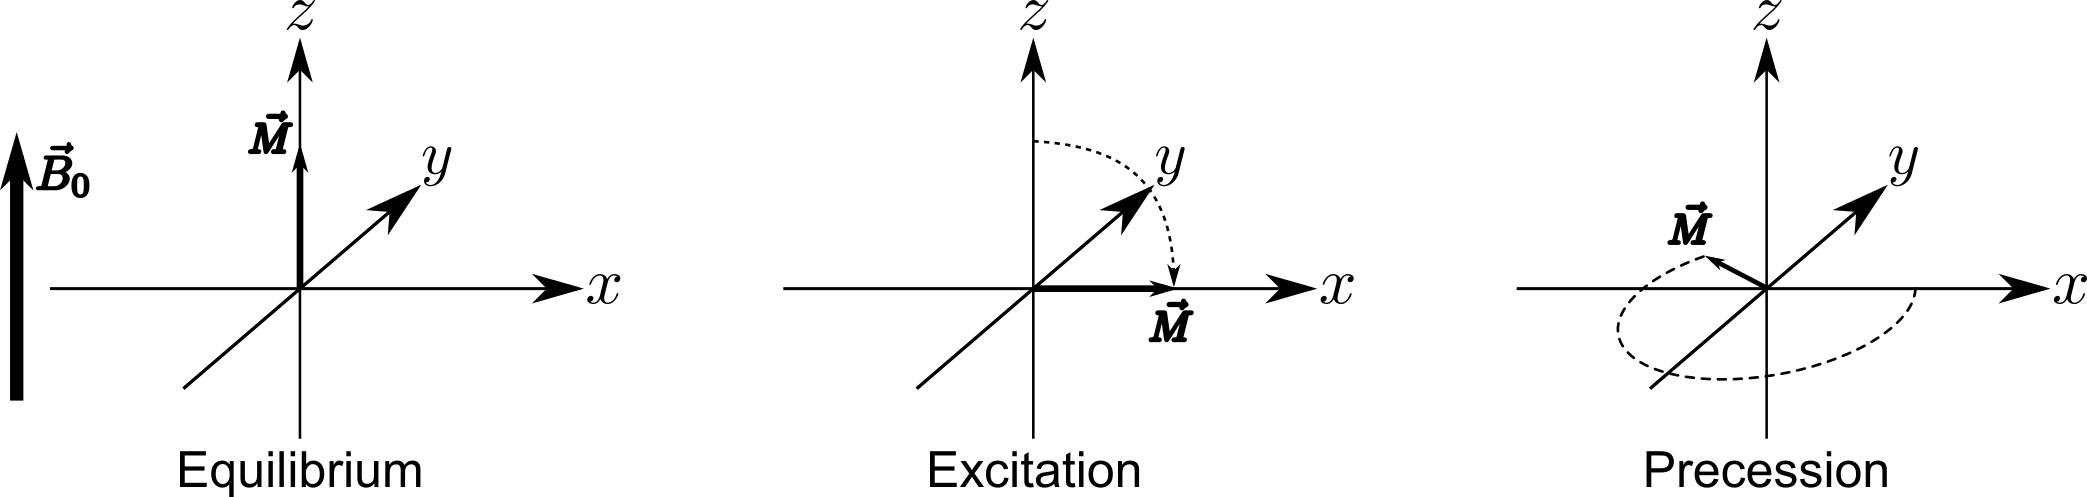
\includegraphics[width=1.0\textwidth]{fig/mri-nmr.png}
  \caption{Illustration of a pulsed NMR experiment on a net magnetization $\vec{M}$: equilibrium, excitation, and precession in the presence of a static magnetic field $\vec{B}_0$.} \label{Fig:mri-nmr}
\end{figure}


\section{Spatial Encoding} \label{Sec:mri-signal-detect}
Once the flipped magnetization starts to precess towards its thermodynamic equilibrium, receiver coils detect an electromotive force (EMF) because they are swept by the magnetized nuclear spins and hence create time-varying currents, which eventually become a meaningful image of the sample. As derived in \cite{1999_MRI},
\begin{align} 
  y(t)  &= -\frac{\text{d}}{\text{d}t} \int_{V} \vec{M} (\vec{r},t) \cdot \vec{B}_{\text{coil}} (\vec{r}) \text{d}^{3} r \nonumber \\
  &\propto \omega_0 \int_{V} \vec{M}_{\perp} (\vec{r},t) c(\vec{r}) e^{- i \omega_0 t} \text{d}^{3} r \label{Equ:mri_emf}
\end{align}
where $V$ denotes the excited volume, and the first term ($\omega_0$) reveals that the Larmor oscillations in the $x$-$y$ plane cause the dominant signal in the receiver coil $c(\vec{r})$. Signals from \cref{Equ:mri_emf}, however, cannot distinguish the excited spatially-varying samples. Thus, magnetic-field gradients are used for the purpose of 2D or 3D imaging. 

First of all, the \textbf{slice selection gradient} (e.g.~$G_z$ as shown in \cref{Fig:mri-slice-sel}) is applied during the RF excitation pulse,
\begin{equation} \label{Equ:mri_slice}
  \gamma \vec{B} = \gamma \vec{B}_0 + \gamma \vec{G} \cdot \vec{r} = \left( \begin{array}{c} 
      0 \\
      0 \\
      \omega_0
    \end{array} \right) + \gamma \cdot \left( \begin{array}{c}
      G_x \\
      G_y \\
      G_z
    \end{array} \right) \cdot \left( \begin{array}{c}
     x \\
     y \\
     z
    \end{array} \right)
\end{equation}
where $\vec{r}$ represents the spatial coordinate of $\vec{M}$ and the altered Larmor frequency ($\omega_z = \omega_0 + \gamma G_{z} z$) linearly changes over the longitudinal direction. In principle, an arbitrarily-oriented slice can be selected by appropriately projecting $G_z$ onto $G_x$, $G_y$, and $G_z$ via a \num{3x3} rotation matrix. On the other hand, in order to select a rectangle-shape slice, which corresponds to a rectangular RF pulse in the spatial frequency domain, the applied RF pulse in the time domain must be a sinc function, as the Fourier transform of a rectangle is a sinc, which is ideally infinite but not applicable in practice. A practical solution is to use the truncated-sinc RF pulse.
\begin{figure}[tb]
  \centering
  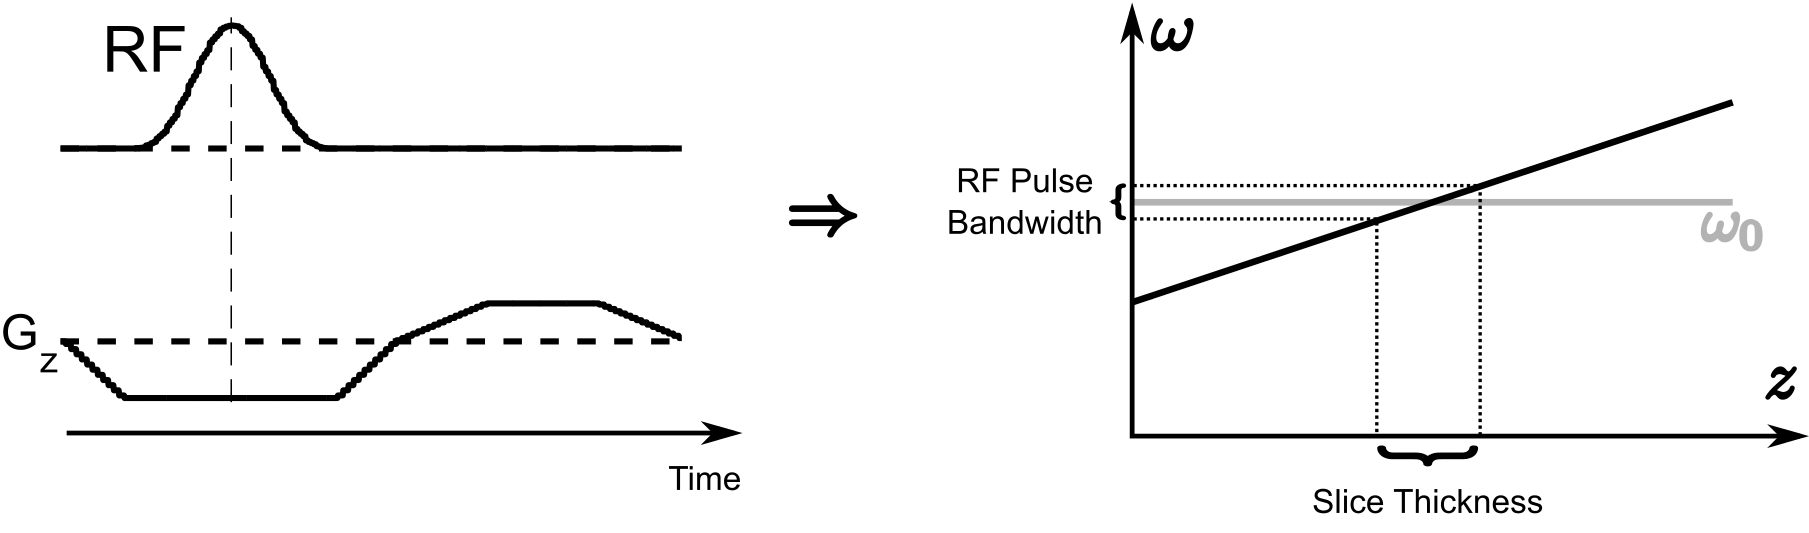
\includegraphics[width=1.0\textwidth]{fig/mri-slice-sel.png}
  \caption{Slice selection: (Left) The application of a truncated sinc RF pulse and slice selection gradient in time domain. (Right) The relation between the selected slice and Larmor frequency.} \label{Fig:mri-slice-sel}
\end{figure}

Second, two \textbf{frequency encoding gradients} ($G_x$ and $G_y$ here) are used to encode signals from every voxel within the selected slice. Similar to \cref{Equ:mri_slice}, the spatial frequency on the selected slice becomes
\begin{equation} \label{Equ:mri_freq}
  w_{\perp} = \gamma G_x \cdot x + \gamma G_y \cdot y
\end{equation}
which can be inserted into \cref{Equ:mri_emf} and yields
\begin{equation} \label{Equ:emf_grad}
  y(t) \propto \omega_0 \int_{V} M_{\perp} (\vec{r},t_{\text{RF}}) \cdot c(\vec{r}) \cdot e^{- i [\omega_0 + \gamma x \int_{0}^{t} G_x(\tau) \text{d}\tau + \gamma y \int_{0}^{t} G_y(\tau) \text{d}\tau] t } \text{d}^{3} r
\end{equation}
where $M_{\perp}(\vec{r}, t_{\text{RF}})$ denotes the transversal magnetization immediately after the RF excitation, while the first ($\omega_0$) and the RF phase ($e^{-i \omega_0 t}$) term is technically removed by retaining the envelope of the detected signal and using a low-pass filter, respectively. Therefore, the spatial-frequency MR signal encoding, known as the k-space sampling, can be simplified as
\begin{equation} \label{Equ:mri_signal}
  y(t) = \int_{V} M_{\perp}(\vec{r}) \cdot c(\vec{r}) \cdot e^{-i 2\pi \cdot \vec{k} (t) \cdot \vec{r}} \text{d} \vec{r}
\end{equation}
where 
\begin{equation} \label{Equ:mri_ktrj}
  \vec{k} (t) := \frac{\gamma}{2\pi} \int_{0}^{t} \vec{G} (\tau) \text{d} \tau
\end{equation}
denoting the k-space sampling trajectory, and $M_{xy}(\vec{r}, t_{\text{RF}})$ is equivalent to \acs{PD}. It can be seen that the received signal in k-space is the Fourier transform of the dot product between PD and the coil sensitivity map.



\section{Imaging Sequences} \label{Sec:mri-seq}
To begin with, it is important to introduce the free induction decay (\acs{FID}), the received NMR signal immediately after the RF excitation, as shown in \cref{Fig:mri-fid}. The envelope of the FID can be approximated by an exponential function with an effective spin-spin relaxation time (\acs{T2s}), 
\begin{equation} \label{Equ:mri_t2s}
  \frac{1}{T_{2}^{*}} = \frac{1}{T_2} + \gamma \cdot \Delta B_0
\end{equation}
where $\Delta B_0$ is the local magnetic field inhomogeneity. Thereby, $T_{2}^{*}$ is even shorter than $T_2$.
\begin{figure}[tb]
  \centering
  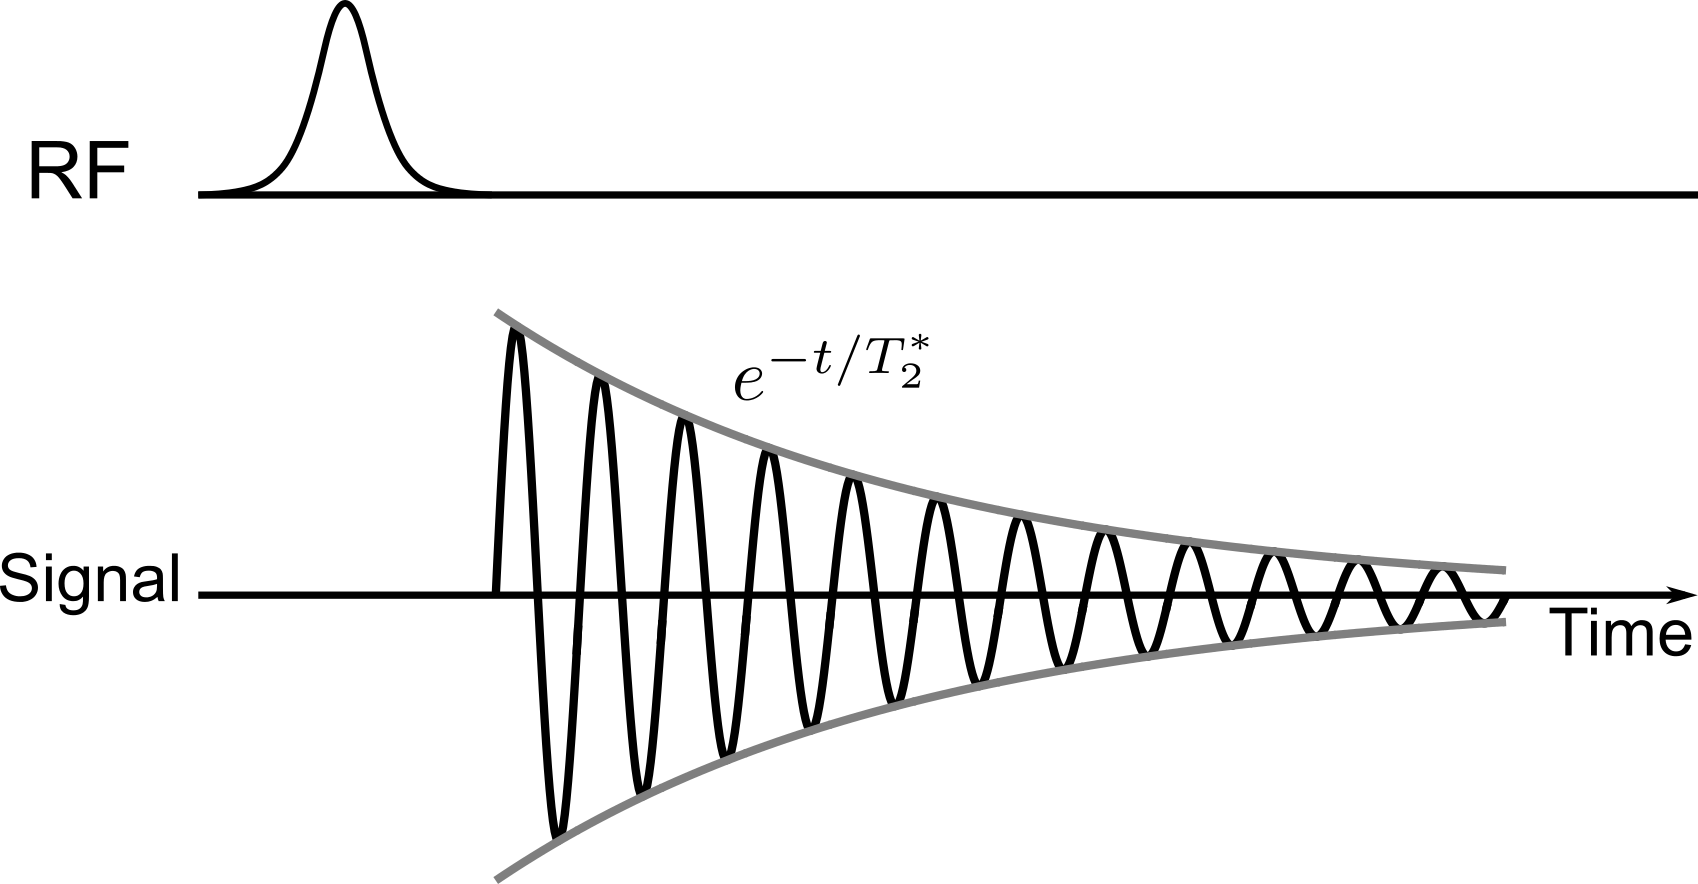
\includegraphics[width=0.6\textwidth]{fig/mri-fid.png}
  \caption{Free induction decay. The oscillating solid line represents the received signal, whose envelop (gray) is the $T_{2}^{*}$ exponential decay curve.} \label{Fig:mri-fid}
\end{figure}

\subsection{Gradient Echo}
A typical spoiled gradient echo sequence for 2D imaging is shown in \cref{Fig:mri-seq-ge-cart}, where one repetition block encodes one echo in k-space. Here, the application of the prephasing gradient adds a spatially-dependent phase term to nuclear spins, which accelerates the FID signal decay because this gradient perturbs the static magnetic field $\vec{B}_0$, produces spatially-varying field inhomogeneities, and leads to faster spin dephasing. The dephased spins, however, can be rephased by a gradient with reversed polarity, namely the readout gradient, during which the analog-to-digital converter (ADC) is switched on to readout signals. When the area of the readout gradient is equal to that of the prephasing gradient, the signal of the central k-space point ($k_x = 0$) is reached. This time point is named as the echo time (\acs{TE}). The sequence block represents one repetition, whose duration is defined as the repetition time (\acs{TR}).
\begin{figure}[tb]
  \centering
  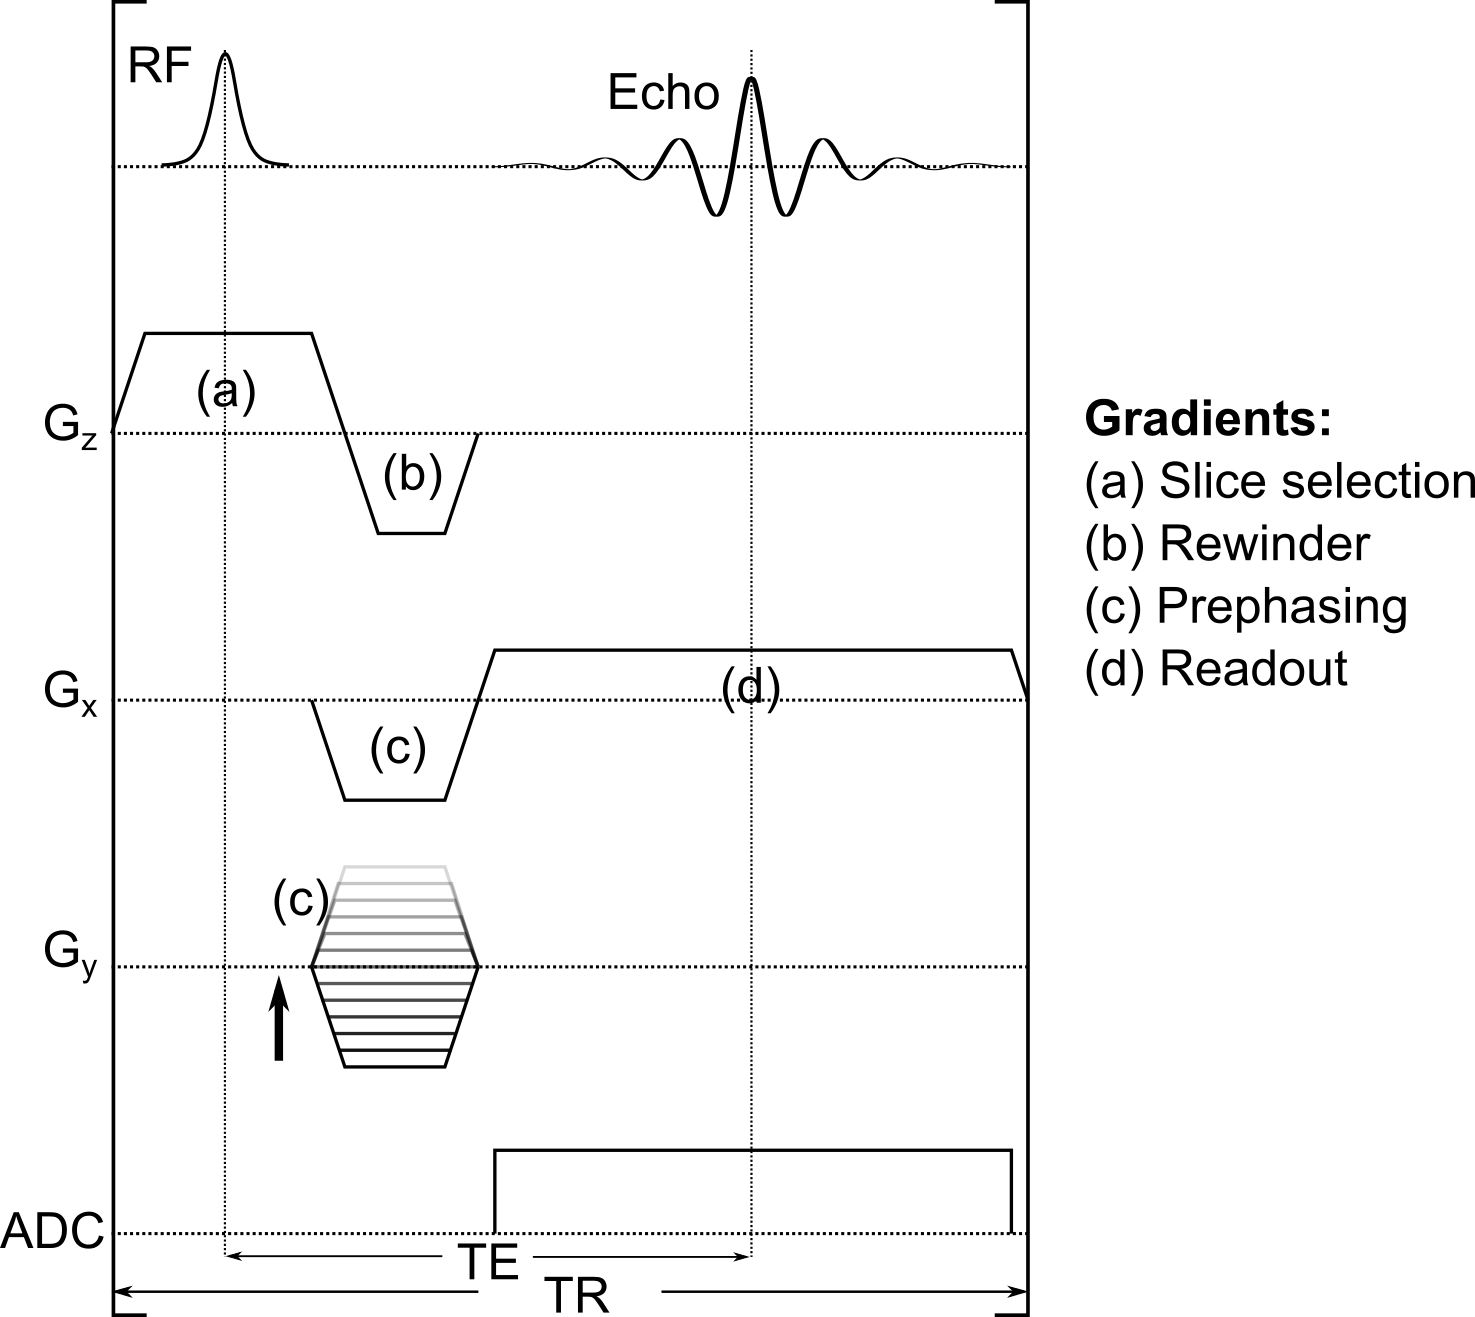
\includegraphics[scale=1]{fig/mri-seq-ge-cart.png}
  \caption{Spoiled gradient echo sequence diagram. For the simplicity of explanation, the imaging slice is the transversal plane. Thus, the $z$ gradient is used for slice selection, while the $x$ and $y$ gradients are used for readout and phase-encoding gradient, respectively. Phase-encoding gradients effectively separate every readout line along the $k_y$ direction.} \label{Fig:mri-seq-ge-cart}
\end{figure}

A specific example of gradient echo sequences is \acs{FLASH}, invented by Frahm et al.~in 1985 \cite{1986_FLASH}. FLASH is a fast imaging technique that reduces MRI measuring times to about hundreds of milliseconds per image due to its extremely short TE and TR. Moreover, the equilibrium magnetization is only slightly flipped towards the transversal plane by a low flip angle (e.g.~\ang{15}).

\subsection{Spin Echo}
Spin echo was discovered by Hahn in 1950 \cite{1950_spin-echo}. A well-known variant of spin echo sequences that has been widely used in clinics is the rapid acquisition with relaxation enhancement (\acs{RARE}) sequence, invented by Hennig et al.~in 1986 \cite{1986_RARE}. As depicted in \cref{Fig:mri-seq-se-cart}, a \ang{90} RF excitation pulse is applied to flip the equilibrium magnetization to the $x$ axis, then a \ang{180} RF pulse is applied at time $\text{TE}/2$ to flip the dephased spins along the $y$ axis, and after the same time period $\text{TE}/2$ spins will be completely rephased again. In this process, the dephasing effect caused by local magnetic field inhomogeneities is compensated by the \ang{180} pulse. Thus, the signals of spin echoes are weighted by $T_2$, instead of $T_2^*$ in gradient echoes. In general, spin echo sequences produce $T_2$-weighted images, in contrast to $T_1$-weighted images from FLASH with relatively shorter TE and TR.
\begin{figure}[tb]
  \centering
  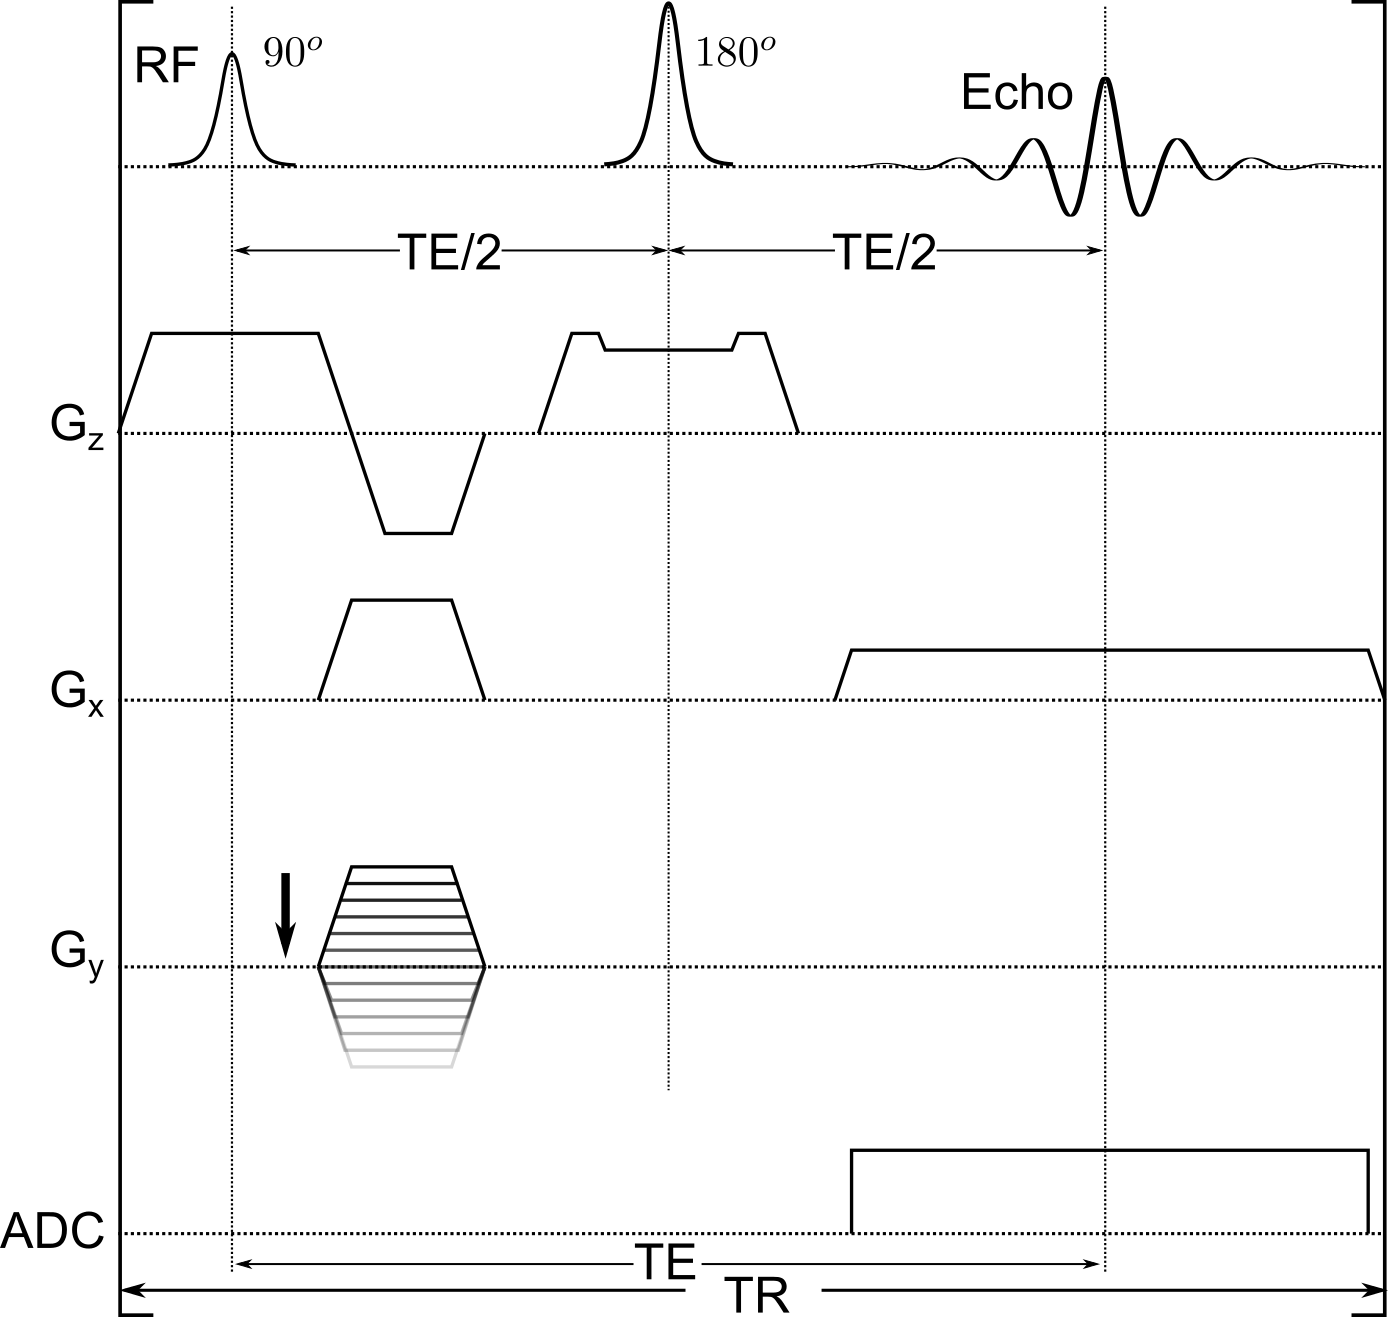
\includegraphics[scale=1]{fig/mri-seq-se-cart.png}
  \caption{Spin echo sequence diagram. Spin dephasing is compensated by a \ang{180} RF pulse that flips all spins along the $y$ axis (assuming that spins are flipped to the $x$ axis by a \ang{90} RF excitation pulse), and thus all spins refocus again on the $x$ axis at the echo time.} \label{Fig:mri-seq-se-cart}
\end{figure}



\section{k-Space Sampling Trajectories} \label{Sec:mri-ktrj}
\begin{figure}[tb]
  \centering
  \subfloat[][Cartesian]{ %
    \label{Fig:mri-trj-cartes} %
    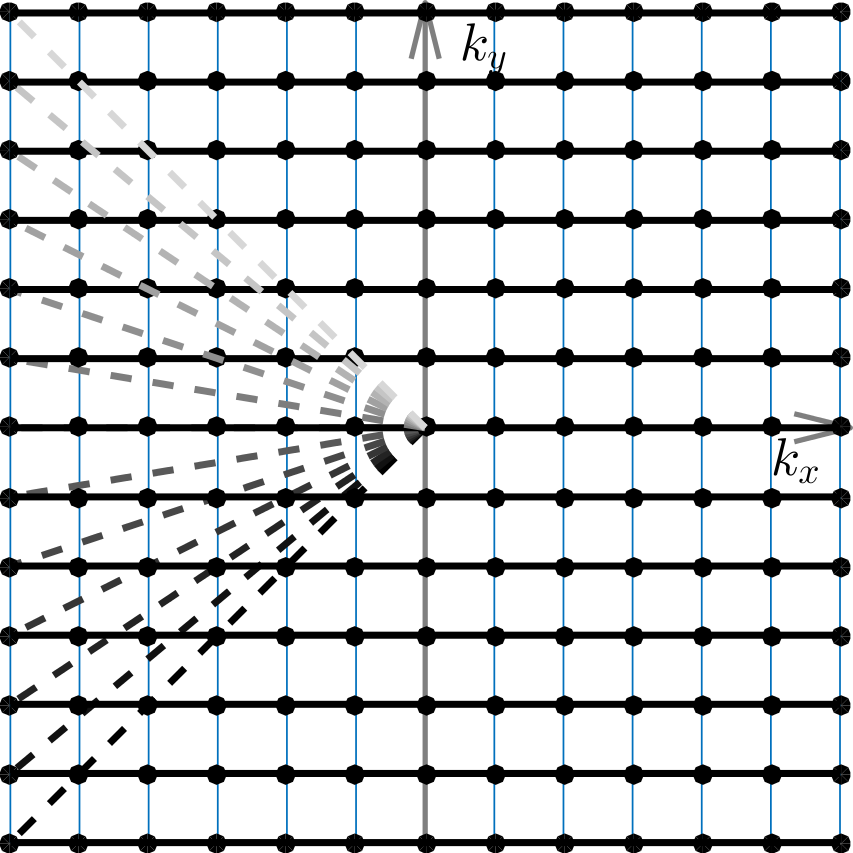
\includegraphics[width=0.3\textwidth]{fig/mri-trj-cartes.png}} \quad
  \subfloat[][Radial]{ %
    \label{Fig:mri-trj-radial} %
    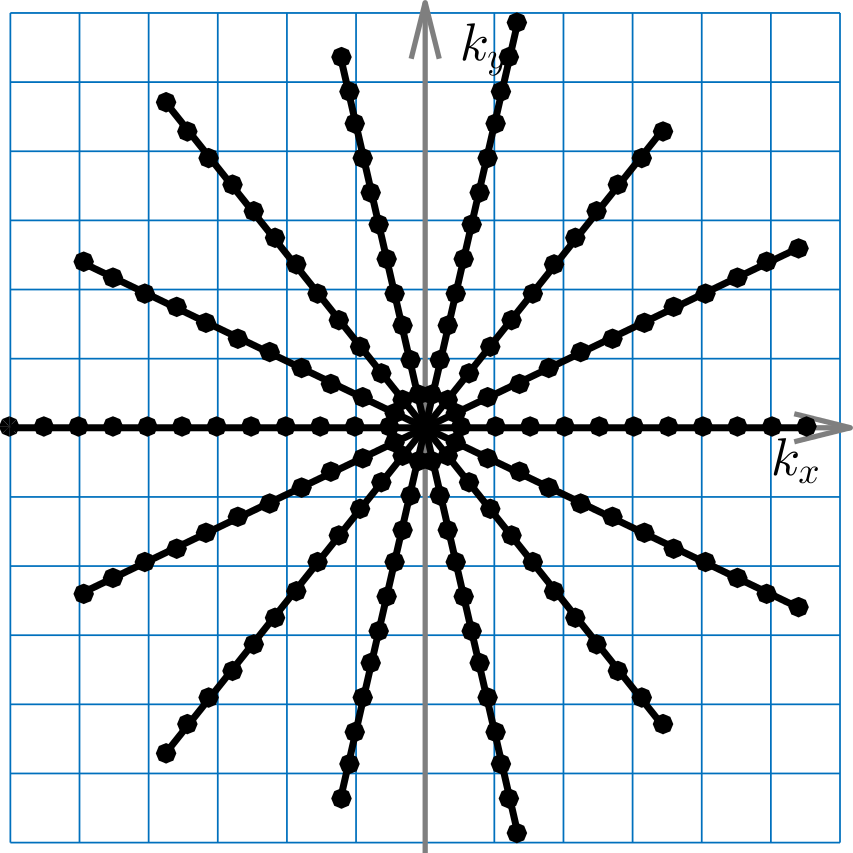
\includegraphics[width=0.3\textwidth]{fig/mri-trj-radial.png}} \\
  \subfloat[][Spiral]{ %
    \label{Fig:mri-trj-spiral} %
    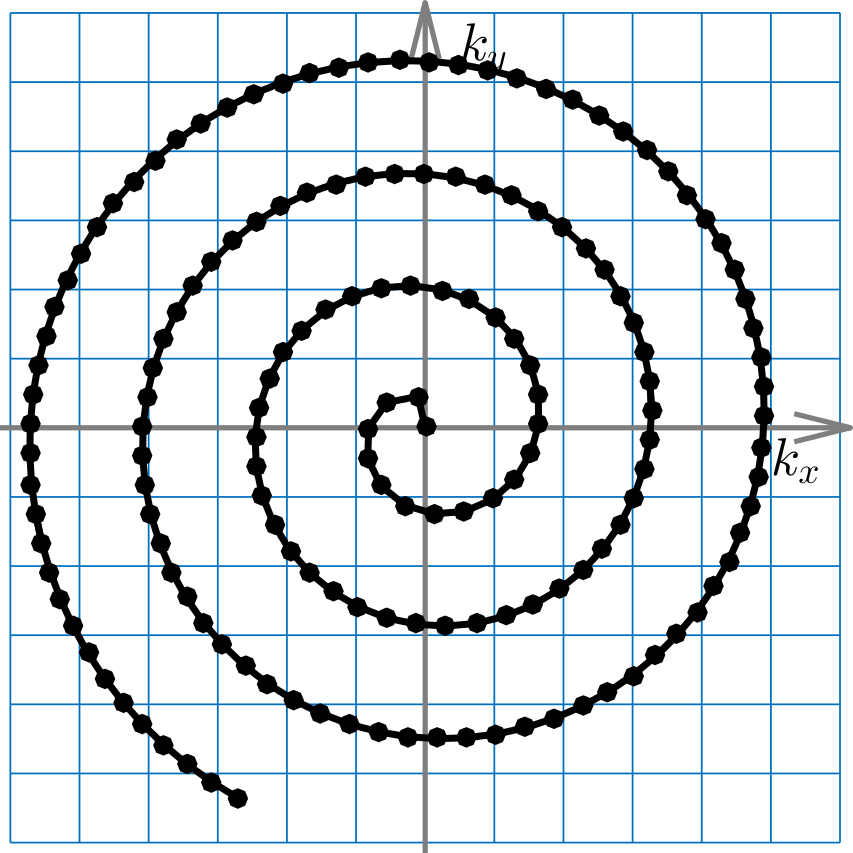
\includegraphics[width=0.3\textwidth]{fig/mri-trj-spiral.png}} \quad
  \subfloat[][Random]{ %
    \label{Fig:mri-trj-random} %
    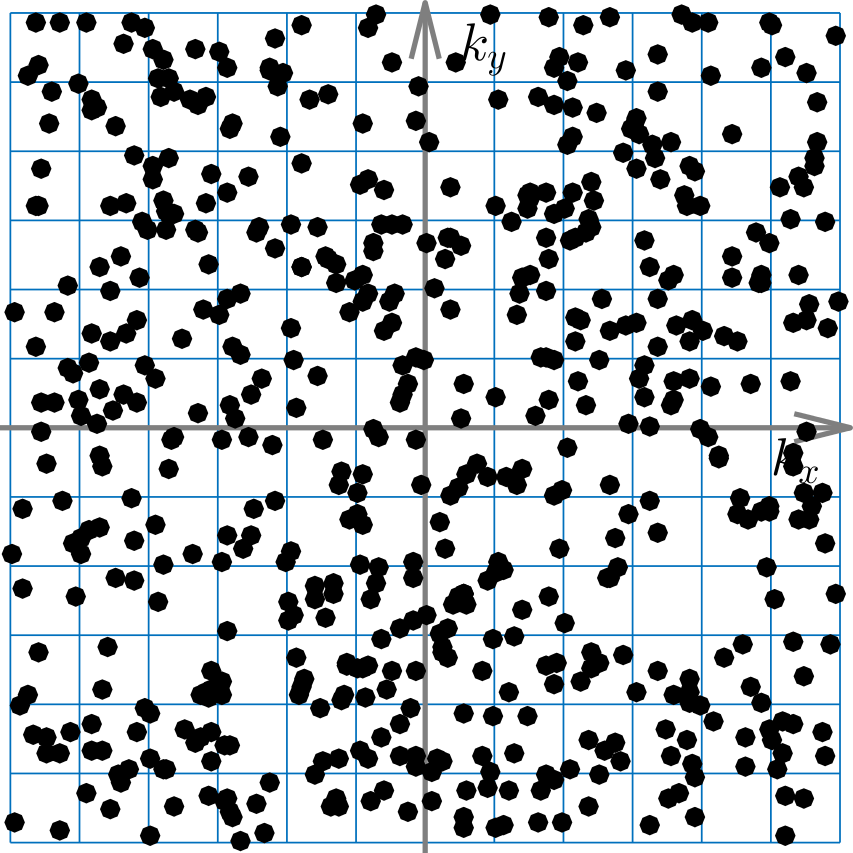
\includegraphics[width=0.3\textwidth]{fig/mri-trj-random.png}} %
  \caption{Schematic illustration of four most popular k-space sampling trajectories. The dashed lines in \protect\subref{Fig:mri-trj-cartes} represent the the trajectories generated by the predephasing and the phase-encoding gradients. The solid lines represent the readout echoes. The intersections of blue lines represent the 2D Cartesian grid.}
  \label{Fig:mri-trj}
\end{figure}
\cref{Fig:mri-trj} depicts four most popular k-space sampling trajectories. According to \cref{Equ:mri_ktrj}, the spoiled gradient echo sequence in \cref{Fig:mri-seq-ge-cart} results in the \textbf{Cartesian} sampling trajectory as shown in \cref{Fig:mri-trj-cartes}, where every sample is located on the Cartesian grid. Thus, a fully-sampled Cartesian dataset mainly requires the fast Fourier transform (\acs{FFT}). Moreover, it is insensitive to gradient delay errors, in which case all echoes in Cartesian sampling have identical phase shifts because the same readout gradient is used for every echo.

The \textbf{radial} sampling trajectory, as shown in \cref{Fig:mri-trj-radial}, has been the very first trajectory proposed for MRI by Lauterbur in 1973 \cite{1973_Nature}, but requires more precise gradient switching because gradient delay errors induce inconsistent phase shifts among echoes. According to \cref{Equ:mri_ktrj}, radial sampling can be accomplished with the following readout gradients,
\begin{equation} \label{Equ:mri_grad_rad}
  \begin{aligned}
    G_x &= G_{\text{max}} \cdot \cos(\theta) \\
    G_y &= G_{\text{max}} \cdot \sin(\theta)
  \end{aligned}
\end{equation}
where $G_{\text{max}}$ is the maximal gradient amplitude, and $\theta$ is the angle of one radial echo (\textit{spoke}). 

As shown in \cref{Fig:mri-trj-spiral}, the \textbf{spiral} sampling trajectory \cite{1999_spiral} can be implemented via
\begin{align}
  \vec{k}(t) &= a \cdot \theta (t) \cdot e^{i \theta (t)} \quad \text{with} \; \theta (t) = \frac{t}{\sqrt{\alpha + (1 - \alpha) \cdot t}} \quad ,  \label{Equ:mri_grad_spi} \\
\intertext{and}
  \vec{G}(t) &= \frac{2\pi}{\gamma} \frac{\text{d}}{\text{d}t} \vec{k}(t) \quad .
\end{align}
Its characteristics were reviewed by Block et al.~in 2005 \cite{2005_spiral_JMRI}. When compared to other k-space sampling trajectories, spiral sampling has longer readouts, which are prone to field-inhomogeneity-induced phase errors. 

The last one is the \textbf{random} sampling trajectory, as shown in \cref{Fig:mri-trj-random}. It receives recent interest because it meets the prerequisite of applying compressed sensing \cite{2006_CS} to MRI image reconstruction -- \textit{incoherent} sampling \cite{2007_Sparse_MRI}. Whereas this scheme is inefficient in 2D trajectories, it can be successfully implemented in combination with 3D sampling schemes, where $G_z$ is also used as a readout gradient and sampled by random ($k_x$, $k_y$) tuples.







\begin{figure}[tb]
  \centering
  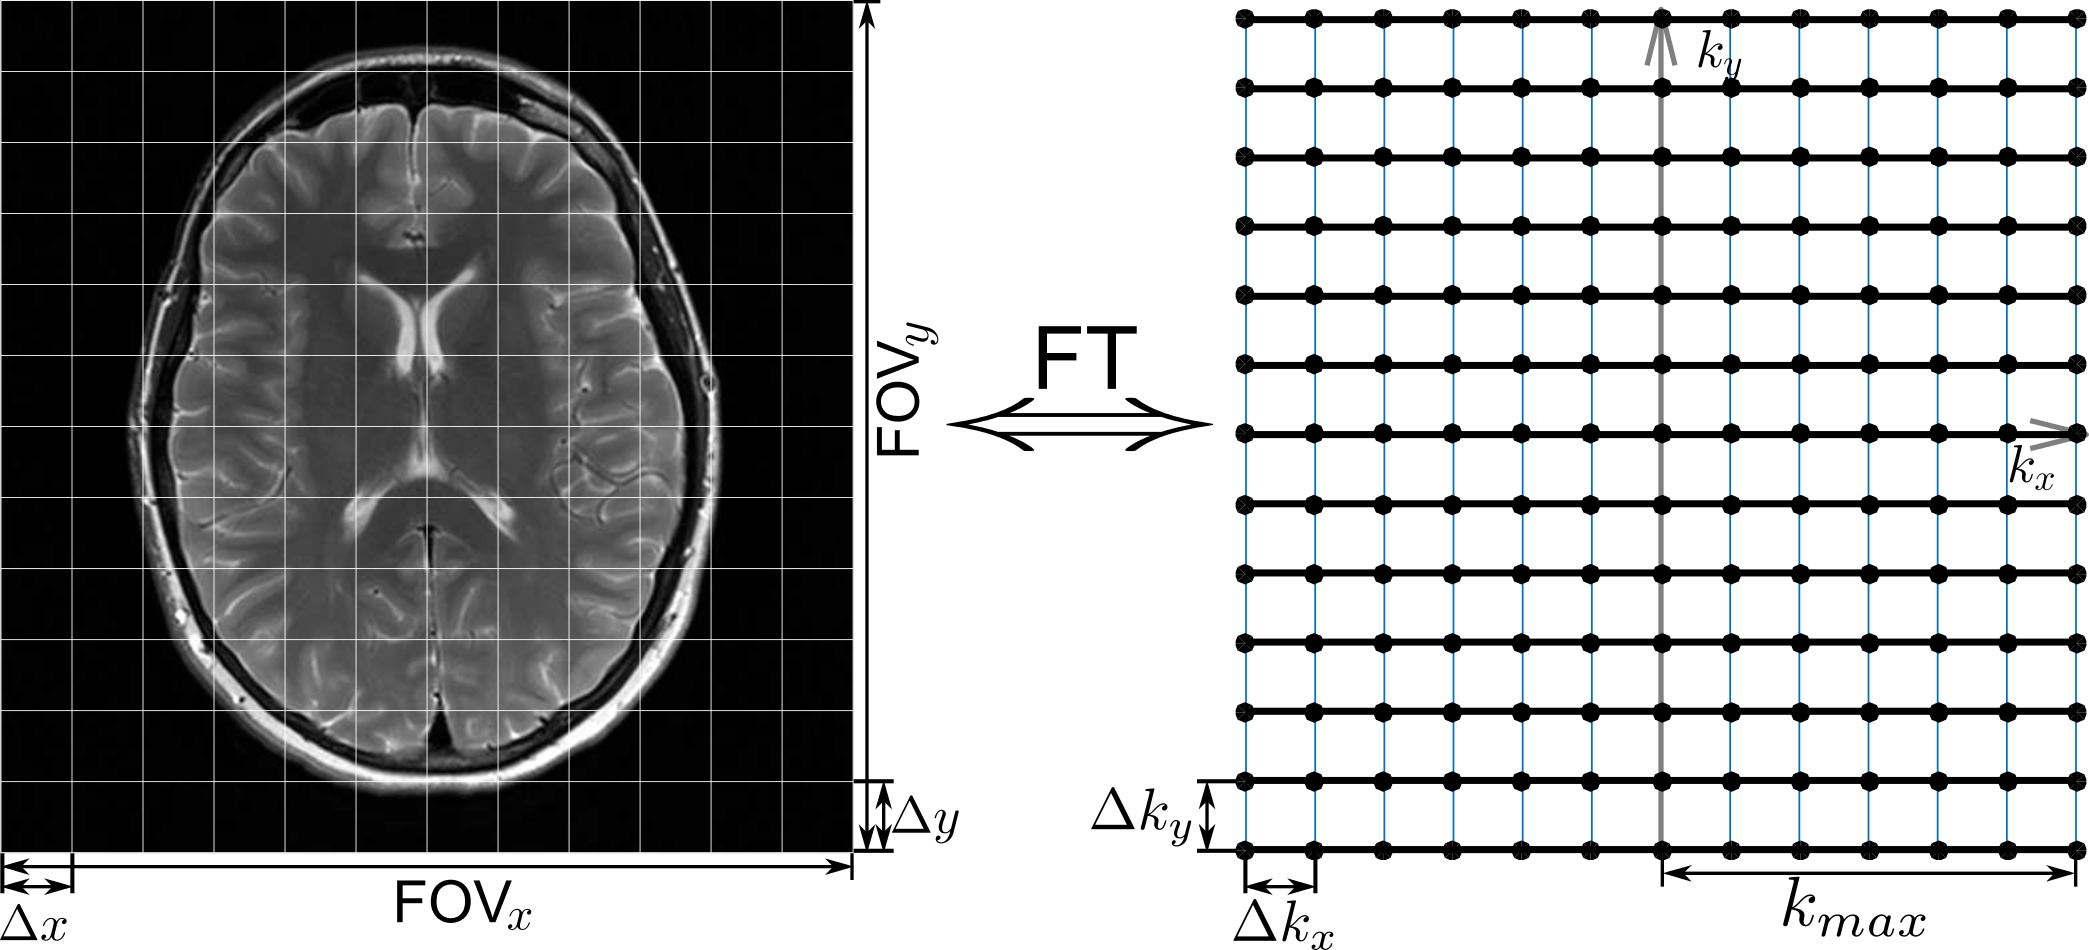
\includegraphics[width=0.8\textwidth]{fig/mri-smp-req.png}
  \caption{Discretization of an image and k-space signal. The image is related to its k-space signal by a Fourier transform.} \label{Fig:mri-smp-req}
\end{figure}
\section{Sampling Requirements}
As shown in \cref{Fig:mri-smp-req}, the continuous k-space signal can be discretized via a Dirac comb function $u(k)$ with the sampling distance ($\Delta k$) 
\begin{align}
  \tilde{y}(k) 
  &= y(k) \cdot u(k) \label{Equ:mri_discrete_y}\\
  &= \Delta k \sum_{p=-\infty}^{\infty} y(p \Delta k) \cdot \delta(k - p \Delta k)
\end{align}
where the inverse Fourier transform of $u(k)$ is
\begin{align}
  U(r) 
  &= \int \Delta k \cdot \delta(k - p \Delta k) \cdot e^{i 2\pi \cdot k \cdot r} \text{d} k \\
  &= \sum_{p=-\infty}^{\infty} \Delta k \cdot e^{i 2\pi \cdot p \Delta k \cdot r}
\end{align}
which only has non-zero values when $r = q / \Delta k$, with $q \in [-\infty,\infty]$, and hence is again a Dirac comb function
\begin{equation}
  U(r) = \delta (r - \frac{q}{\Delta k}) \quad .
\end{equation}
Following \cref{Equ:mri_discrete_y}, the corresponding discrete image is
\begin{align}
  \tilde{\rho}(r) 
  &= \mathcal{F}^{-1} \{ y(k) \cdot u(k) \} \\
  &= \rho(r) \ast U(r) \\
  &= \rho(r) \ast \delta (r - \frac{q}{\Delta k})
\end{align}
with $\ast$ the convolution. It can be seen that $\tilde{\rho}(r)$ is an infinite and periodic function with the period
\begin{equation} \label{Equ:mri_fov}
  r_T = 1 / \Delta k := \text{FOV}
\end{equation} 
where the field-of-view (\acs{FOV}), i.e., the selected image plane (e.g.~in \si{\square\mm}), consists of only one period of $\tilde{\rho}(r)$. Moreover, the discrete $\rho(r)$ is composed of thousands of image elements (pixels), whose size ($\Delta r$), typically defined as the spatial resolution, is given as
\begin{equation} \label{Equ:mri_pixel}
  \Delta r = \frac{\text{FOV}}{N} = \frac{1}{\Delta k \cdot N} = \frac{1}{2k_{\text{max}}}
\end{equation}
with $N$ the number of samples per echo and $k_{\text{max}}$ the maximal k-space sampling position. 

Alternatively, according to \cref{Equ:mri_ktrj}, $\Delta k$ can also be written as
\begin{equation} \label{Equ:mri_smp_int}
  \Delta k_x = \frac{\gamma}{2\pi} G_x \Delta t_x \quad \text{and} \quad \Delta k_y = \frac{\gamma}{2\pi} G_y \Delta t_y
\end{equation}
where $\Delta t_x$ and $\Delta t_y$ is the sampling interval (dwell time) along the $G_x$ and $G_y$ direction, respectively. \cref{Equ:mri_smp_int} indicates how much time is required to encode one k-space sample, so the sampling rate is $1 / \Delta k$, which, according to the Nyquist-Shannon sampling theorem, has to satisfy the following condition in order to avoid the image aliasing artifact,
\begin{equation}
  \Delta k = \frac{2 k_{\text{max}}}{N} \leq \frac{1}{\text{FOV}} \quad . 
\end{equation}
Here, the reduction of $\Delta k_x$ along the readout direction does not increase the measuring time but enlarges the aliasing-free area. 

Further, $\Delta k$ in \cref{Equ:mri_smp_int} is determined by two factors: the gradient strength and the dwell time. For fixed $\Delta k$ and $k_{\text{max}}$, a reduced gradient strength prolongs the dwell time and also the total readout duration, yielding a higher signal-to-noise ratio (SNR). The reciprocal of $\Delta t$ is represented by the receiver bandwidth (\acs{BW}). Therefore, the higher the bandwidth, the faster the sampling rate, and the lower the \acs{SNR} \cite{2009_Zhang_Thesis}. 


\section{Gridding \& FFT Image Reconstruction} \label{Sec:mri_grid}
In the case of Cartesian sampling, an inverse \acs{FFT} can be directly applied to the sampled k-space data to obtain an image. For non-Cartesian sampling trajectories (e.g.~radial and spiral), however, the sampled k-space data are not necessarily located on the Cartesian grid. As a result, the image reconstruction of k-space data from non-Cartesian sampling requires the non-uniform FFT (\acs{NUFFT}) \cite{2003_NUFFT}, known as the \textbf{gridding} algorithm in MRI \cite{1991_conv_gridding,1999_gridding_TMI,2005_gridding,2008_Block_Thesis}, to interpolate the data onto the Cartesian grid prior to the uniform inverse FFT. In principle, the gridding algorithm includes the following steps
\begin{enumerate}
\item Density compensation. As the sampling density in non-Cartesian trajectories may not be equally distributed in k-space, so a density compensation function (DCF) is required to properly weight every k-space data;
\item Convolution. The density-compensated data is convolved with a window function (e.g.~the Kaiser-Bessel function) with a finite width to interpolate every sample onto its neighboring Cartesian grid, whose minimal sampling distance ($\Delta k_{\text{min}}$) of the Cartesian grid can be smaller than that ($\Delta k$) of the non-Cartesian sampling trajectory. The ratio between them is denoted as the over-gridding ratio $o = \Delta k / \Delta k_{\text{min}}$, which is helpful in reducing image aliasing artifacts;
\item Roll-off correction. Note that the convolution in k-space in the previous step is equivalent to a dot product between the object and the inverse FFT of the window in image domain. Thus, a reconstructed image is obtained by a 2D inverse FFT of the gridded data and then divided by the inverse Fourier transform of the window function. Finally, the image is cropped according to the over-gridding ratio.
\end{enumerate}



\section{Parallel Imaging} \label{Sec:mri_pi}
One main problem in MRI is the imaging speed. Even with the Cartesian FLASH sequence, about one second is required to obtain one image. This temporal resolution is not fast enough for the study of fast physiological motions, e.g.~beating heart. To speed up MRI, data undersampling is a feasible approach, but undersampled k-space results in aliased images. To overcome this problem, parallel imaging has been of great interest ever since the development of phased-array coils \cite{1990_phased_array}, which are usually placed around the subject in order to simultaneously receive k-space data. 

As shown in \cref{Fig:mri-pi}, the coils are more sensitive to signals near to their locations. The spatially-varying sensitivities of the coils are named the \textbf{coil sensitivity map}, in correspondence to which even the aliased coil images due to the two-fold undersampling exhibit brighter intensities in respective regions. This is a direct indication that parallel imaging with multiple receiver coils creates redundant information which can be used to estimate an un-aliased image and hence eventually accelerates data acquisition. The forward operation in parallel imaging can be mathematically denoted as
\begin{equation} \label{Equ:mri-pi-forward}
  F: x \mapsto \left( \begin{array}{c}
    P \mathcal{F} \{ \rho \cdot c_1 \} \\
    \vdots \\
    P \mathcal{F} \{ \rho \cdot c_N \} \\
  \end{array} \right)
\end{equation}
where $\rho$ is the image, $c_n$ is the $n^{\text{th}}$ coil sensitivity map, $\mathcal{F}$ is the 2D FFT, and $P$ is the sampling pattern. On the contrary, the task of the inverse problem posed by parallel imaging is to estimate an un-aliased image and/or a set of coil sensitivity maps via the undersampled multi-coil data and the sampling pattern.
\begin{figure}[tb]
  \centering
  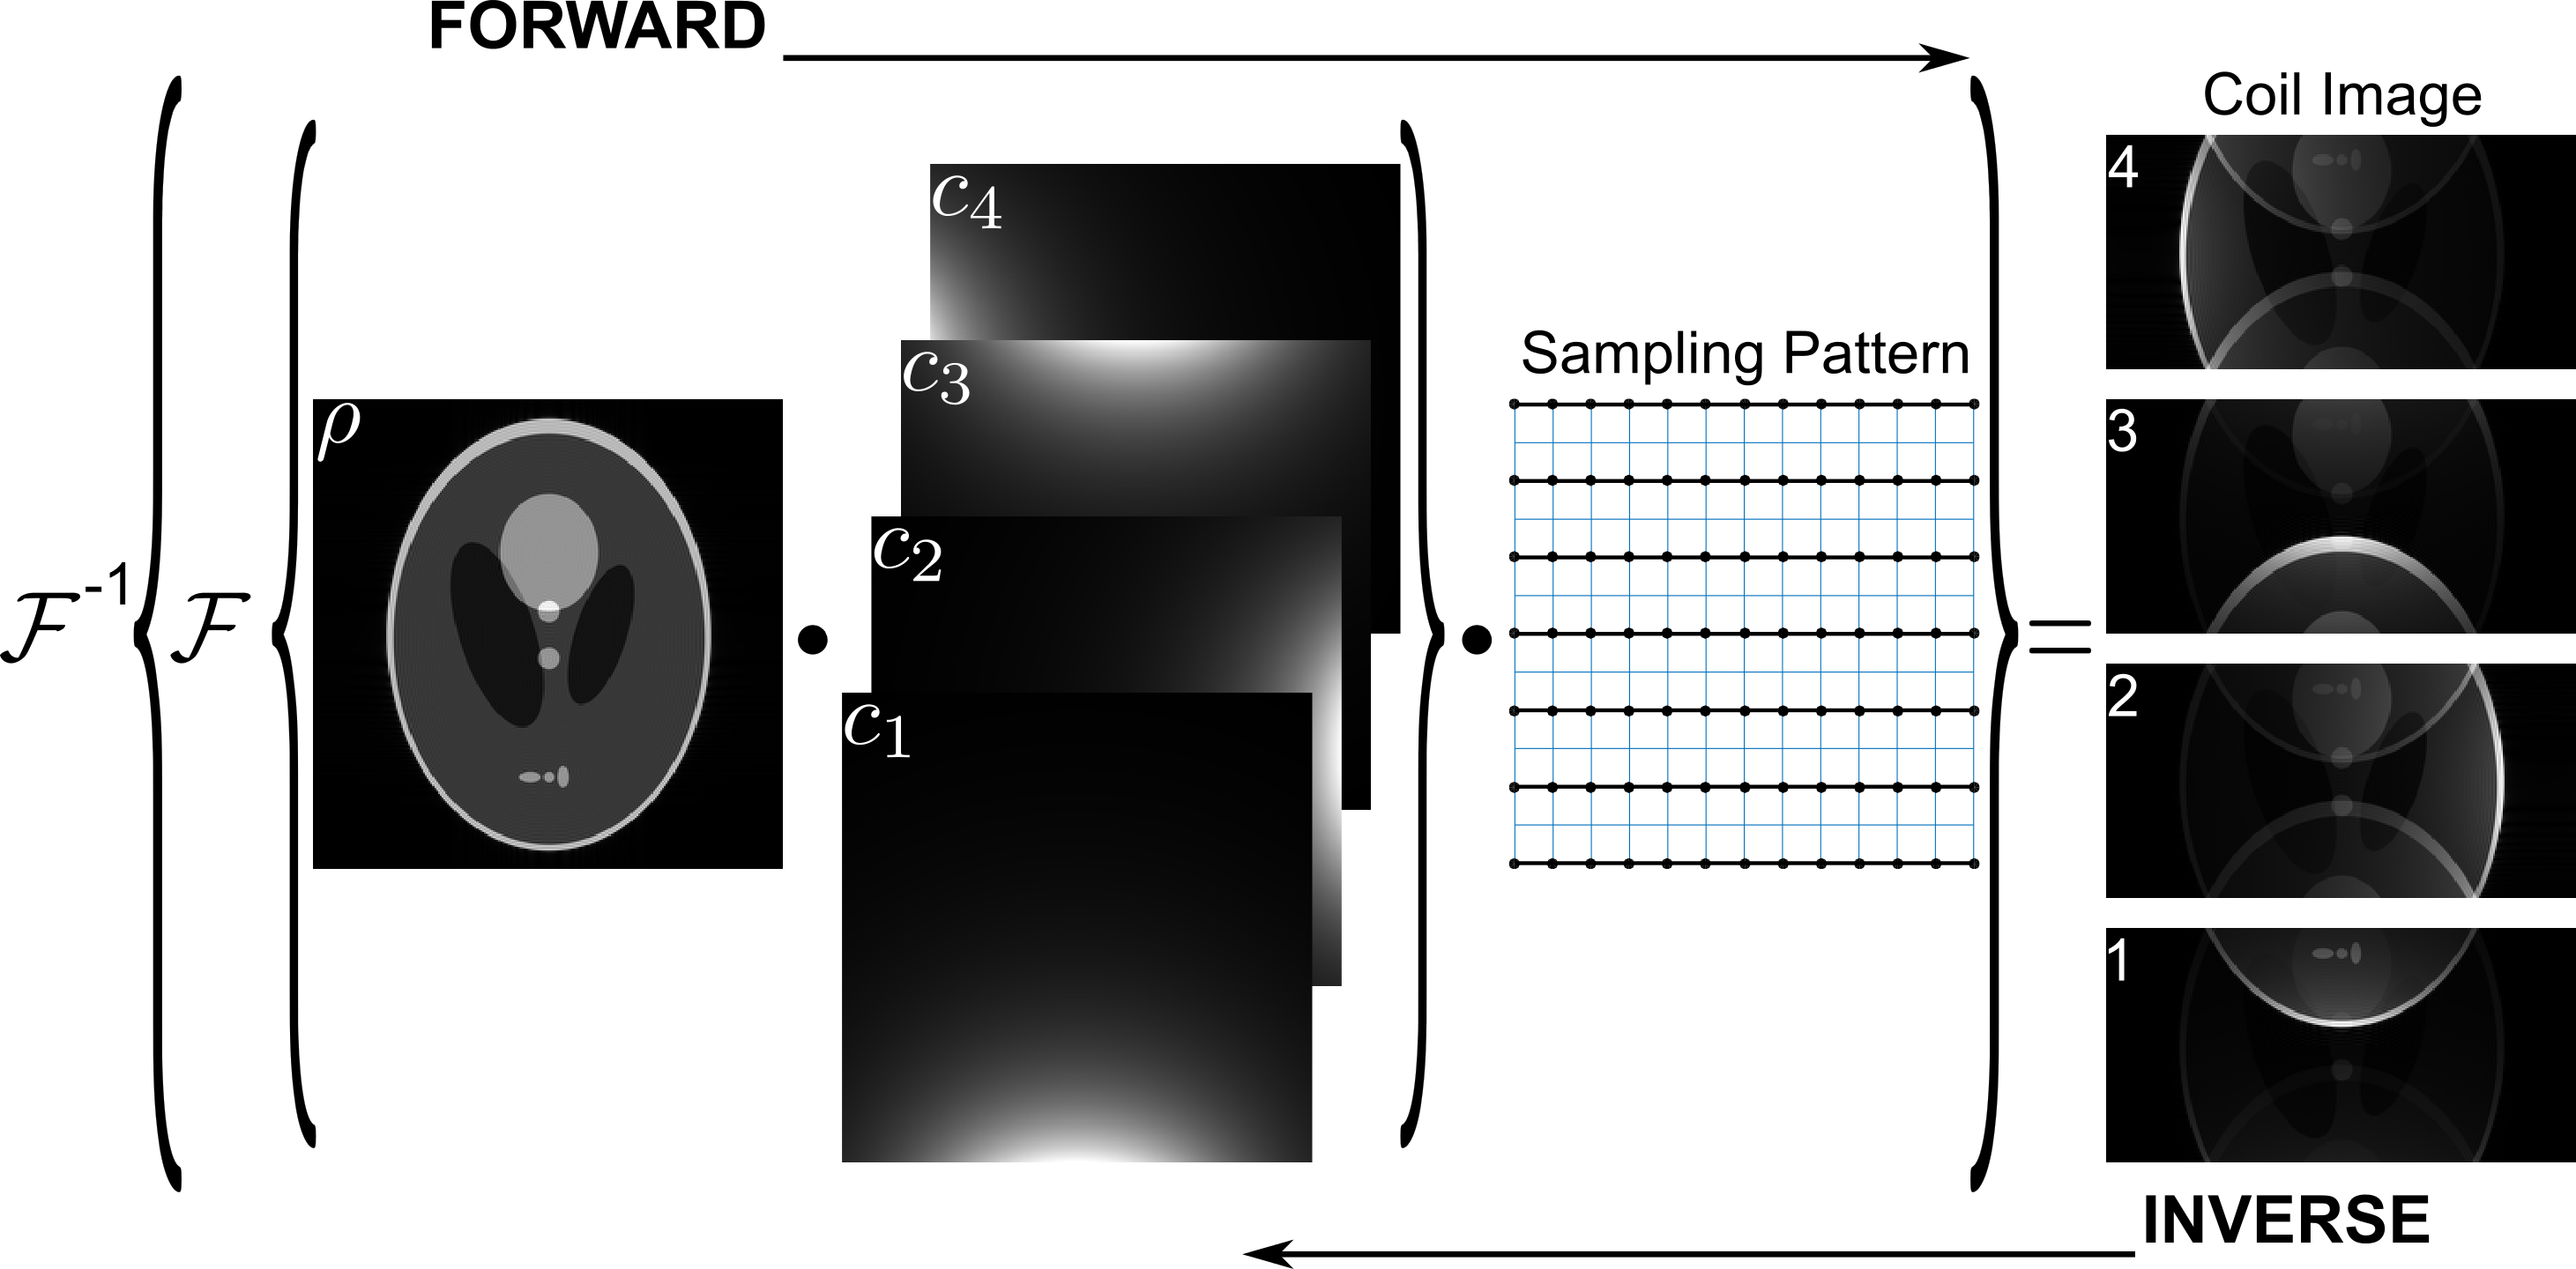
\includegraphics[width = 1.0\textwidth]{fig/mri-pi.png}
  \caption{Schematic illustration of parallel imaging. The forward model can be understood as the 2D FFT ($\mathcal{F}$) of the dot product between the image $\rho$ and every coil sensitivity map evaluated on the sampling pattern. In case of undersampling (as depicted in the sampling pattern, two-fold undersampling is used here), the direct FFT gives aliased coil images. Inverse problem is to estimate an un-aliased image and/or coil sensitivity maps given the undersampled multi-coil data and the sampling pattern.} \label{Fig:mri-pi}
\end{figure}

There exists three generic reconstruction techniques for parallel imaging, sensitivity encoding (\acs{SENSE}) \cite{1999_SENSE,2001_gSENSE}, simultaneously acquisition of spatial harmonics (\acs{SMASH}) \cite{1997_SMASH}, and generalized autocalibrating partially parallel acquisitions (\acs{GRAPPA}) \cite{2002_GRAPPA}, all of which have been commercialized and used in routine clinic. 

The generalized SENSE treats parallel imaging as a linear inverse problem which intends to optimize the following cost function
\begin{equation} \label{Equ:mri_inv_cost}
  \Phi(x) = \argmin\limits_x \sum_{n=1}^{N} \norm{y_n - F(\rho \cdot c_n)}_2^2 + \alpha \norm{\rho}_2^2 \quad \text{with} \; x = \rho \quad .
\end{equation}
Prior to solving this function, the coil sensitivity maps need to be calculated via either a calibration scan or the auto-calibration signal (\acs{ACS}). ACS is usually accomplished by fully sampling the low-spatial-frequency region while the rest of k-space remains undersampled according to the user-defined reduction factor $R$. Non-Cartesian trajectories such as spiral and radial, however, offer inherent self-calibrating signals due to their densely sampled center \cite{2005_self_cal_pi}. With coil sensitivity maps, the above function can be solved by conjugate gradient (\acs{CG}) method and thus this method is dubbed as CG-SENSE. Moreover, due to the ill-condition of the inverse problem, Tikhonov regularization that penalizes the $L^2$ norm of the estimate image is used. 

Recent progress in compressed sensing \cite{2006_CS} has enabled the application of $L^1$-norm regularizations into SENSE-type iterative image reconstructions. $L^1$-norm regularizations are preferable for estimating sparse images, which are achievable via incoherent sampling and sparsifying transforms (e.g.~wavelet). As a result, $L^1$-norm regularizations produce fewer coefficients with non-zero values due to the stronger penalties on small-value coefficients compared to $L^2$-norm regularizations. 

One important variant of SENSE is $k$-$t$ SENSE \cite{2003_k-t_SENSE}, proposed by Tsao et al.~in 2003 for dynamic imaging with high frame rates. Here, $k$ and $t$ refer to the phase-encoding index and acquisition time, respectively. With 1D FFT on $k$ and $t$ respectively, the data in $x$-$f$ space can be obtained. $k$-$t$ SENSE consists of two reconstruction steps. The first step is named the training stage, where a dataset in the low spatial frequency region is acquired and then a signal covariance matrix in $x$-$f$ space is determined. This matrix is considered to be consistent and is thereby used in the second step (acquisition stage) to reconstruct undersampled data.

In contrast, both SMASH and GRAPPA are based on the assumption that a k-space data point is highly correlated with its neighbors, so the missing data can be a linear combination of neighboring signals with appropriate weights. The weights are determined by fitting undersampled k-space data to the ACS. Afterwards, both the undersampled data used in the fitting and the weights are utilized to composite the missing data. GRAPPA-type image reconstructions result in uncombined coil images, which can be combined via either sum of squares \cite{1990_phased_array} or phase-preserving coil combination algorithms \cite{2000_coil_comb}.


\section{MRI System}
As shown in \cref{Fig:mri-sys}, the studies presented in this thesis were conducted at a commercial scanner (MAGNETOM Prisma, Siemens Healthcare\footnote{\url{www.healthcare.siemens.com}}, Erlangen, Germany) with a superconducting magnet of field strength $\abs{\vec{B}_0} = \num{3}$~Tesla (\si{\tesla}) and two built-in body coils for RF excitation and signal receiving. Moreover, the gradient system has a maximal gradient strength of \SI{80}{\milli\tesla\per\meter}. For the gradient switching, the raster time can be as fast as \SI{10}{\micro\second}, and the maximal slew rate is \SI{200}{\tesla\per\meter\per\second}. In addition, the receiver coils used are the \num{64}-channel head coil, the \num{18}-element thorax coil, and the \num{32}-channel spine coil.
\begin{figure}[tb]
  \centering
  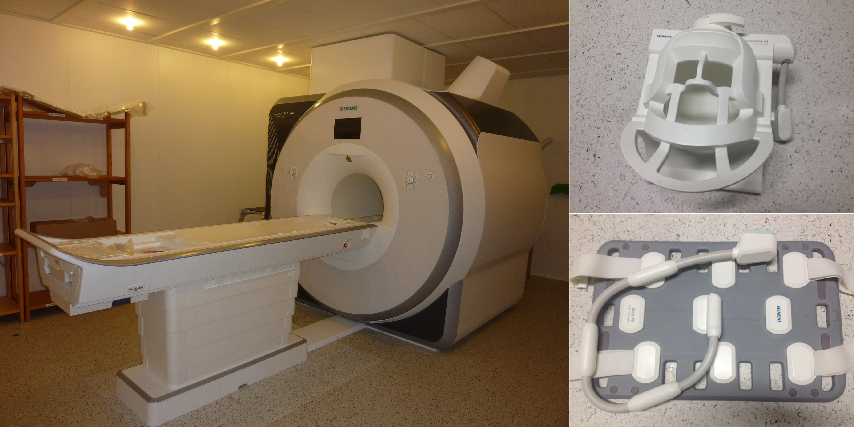
\includegraphics[width = 1.0\textwidth]{fig/mri-sys.png}
  \caption{(Left) MRI system and (right) receiver coils. (Top right) 64-channel head coil and (bottom right) 18-element thorax coil.} \label{Fig:mri-sys}
\end{figure}



\chapter{Real-Time MRI: State of the Art} \label{Chp:rtMRI}
\chaptermark{Real-Time MRI}

Real-time MRI refers to high-speed MRI acquisitions at millisecond resolution. Initially, spiral sampling was proposed for real-time cardiac MRI \cite{2004_rt_spiral} and further developed in HeartVista\texttrademark\footnote{\url{https://www.heartvista.com/}}. For accelerated MRI acquisitions, spiral sampling usually has long readouts, which are prone to off-resonance-induced image artifacts (e.g.~see \cref{Sec:mri-ktrj}). Therefore, this chapter focuses on the real-time \acs{MRI} technique developed in Biomedizinische NMR Forschungs GmbH\footnote{\url{http://www.biomednmr.mpg.de/}}. Essentially, this technique comprises highly undersampled radial \acs{FLASH} acquisitions without any physiological triggering and the nonlinear inverse image reconstruction that accurately estimates both the object image and the coil sensitivity maps. 


\section{Undersampled Radial FLASH} \label{Sec:rtmri-rfl}
Radial sampling has regained great interest in the last decade. First, it is less sensitive to motion-induced ghost artifacts as commonly seen in Cartesian sampling, because the center of k-space is measured by every spoke. However, rapid motions may cause streaking artifacts in radial sampling. Second, radial sampling is resistant to spatial distortion in case of undersampling. Undersampling induces radial streaks as well, which, however, has been proven incoherent and hence can be better suppressed than coherent artifacts (e.g.~the aliasing or fold-in artifact in Cartesian undersampling). Third, as radial sampling contains two readout gradients (see \cref{Equ:mri_grad_rad}) rather than one readout and one phase-encoding gradient, it is feasible to employ oversampling along the readout directions, which effectively enlarges the circular-supported \acs{FOV} and hence reduces aliasing artifacts without additional measuring times. Due to these favorable properties, undersampled radial FLASH was proposed by Zhang et al.~in 2010 \cite{2010_rfl_JMRI} for real-time MRI.

\begin{figure}[tb]
  \centering
  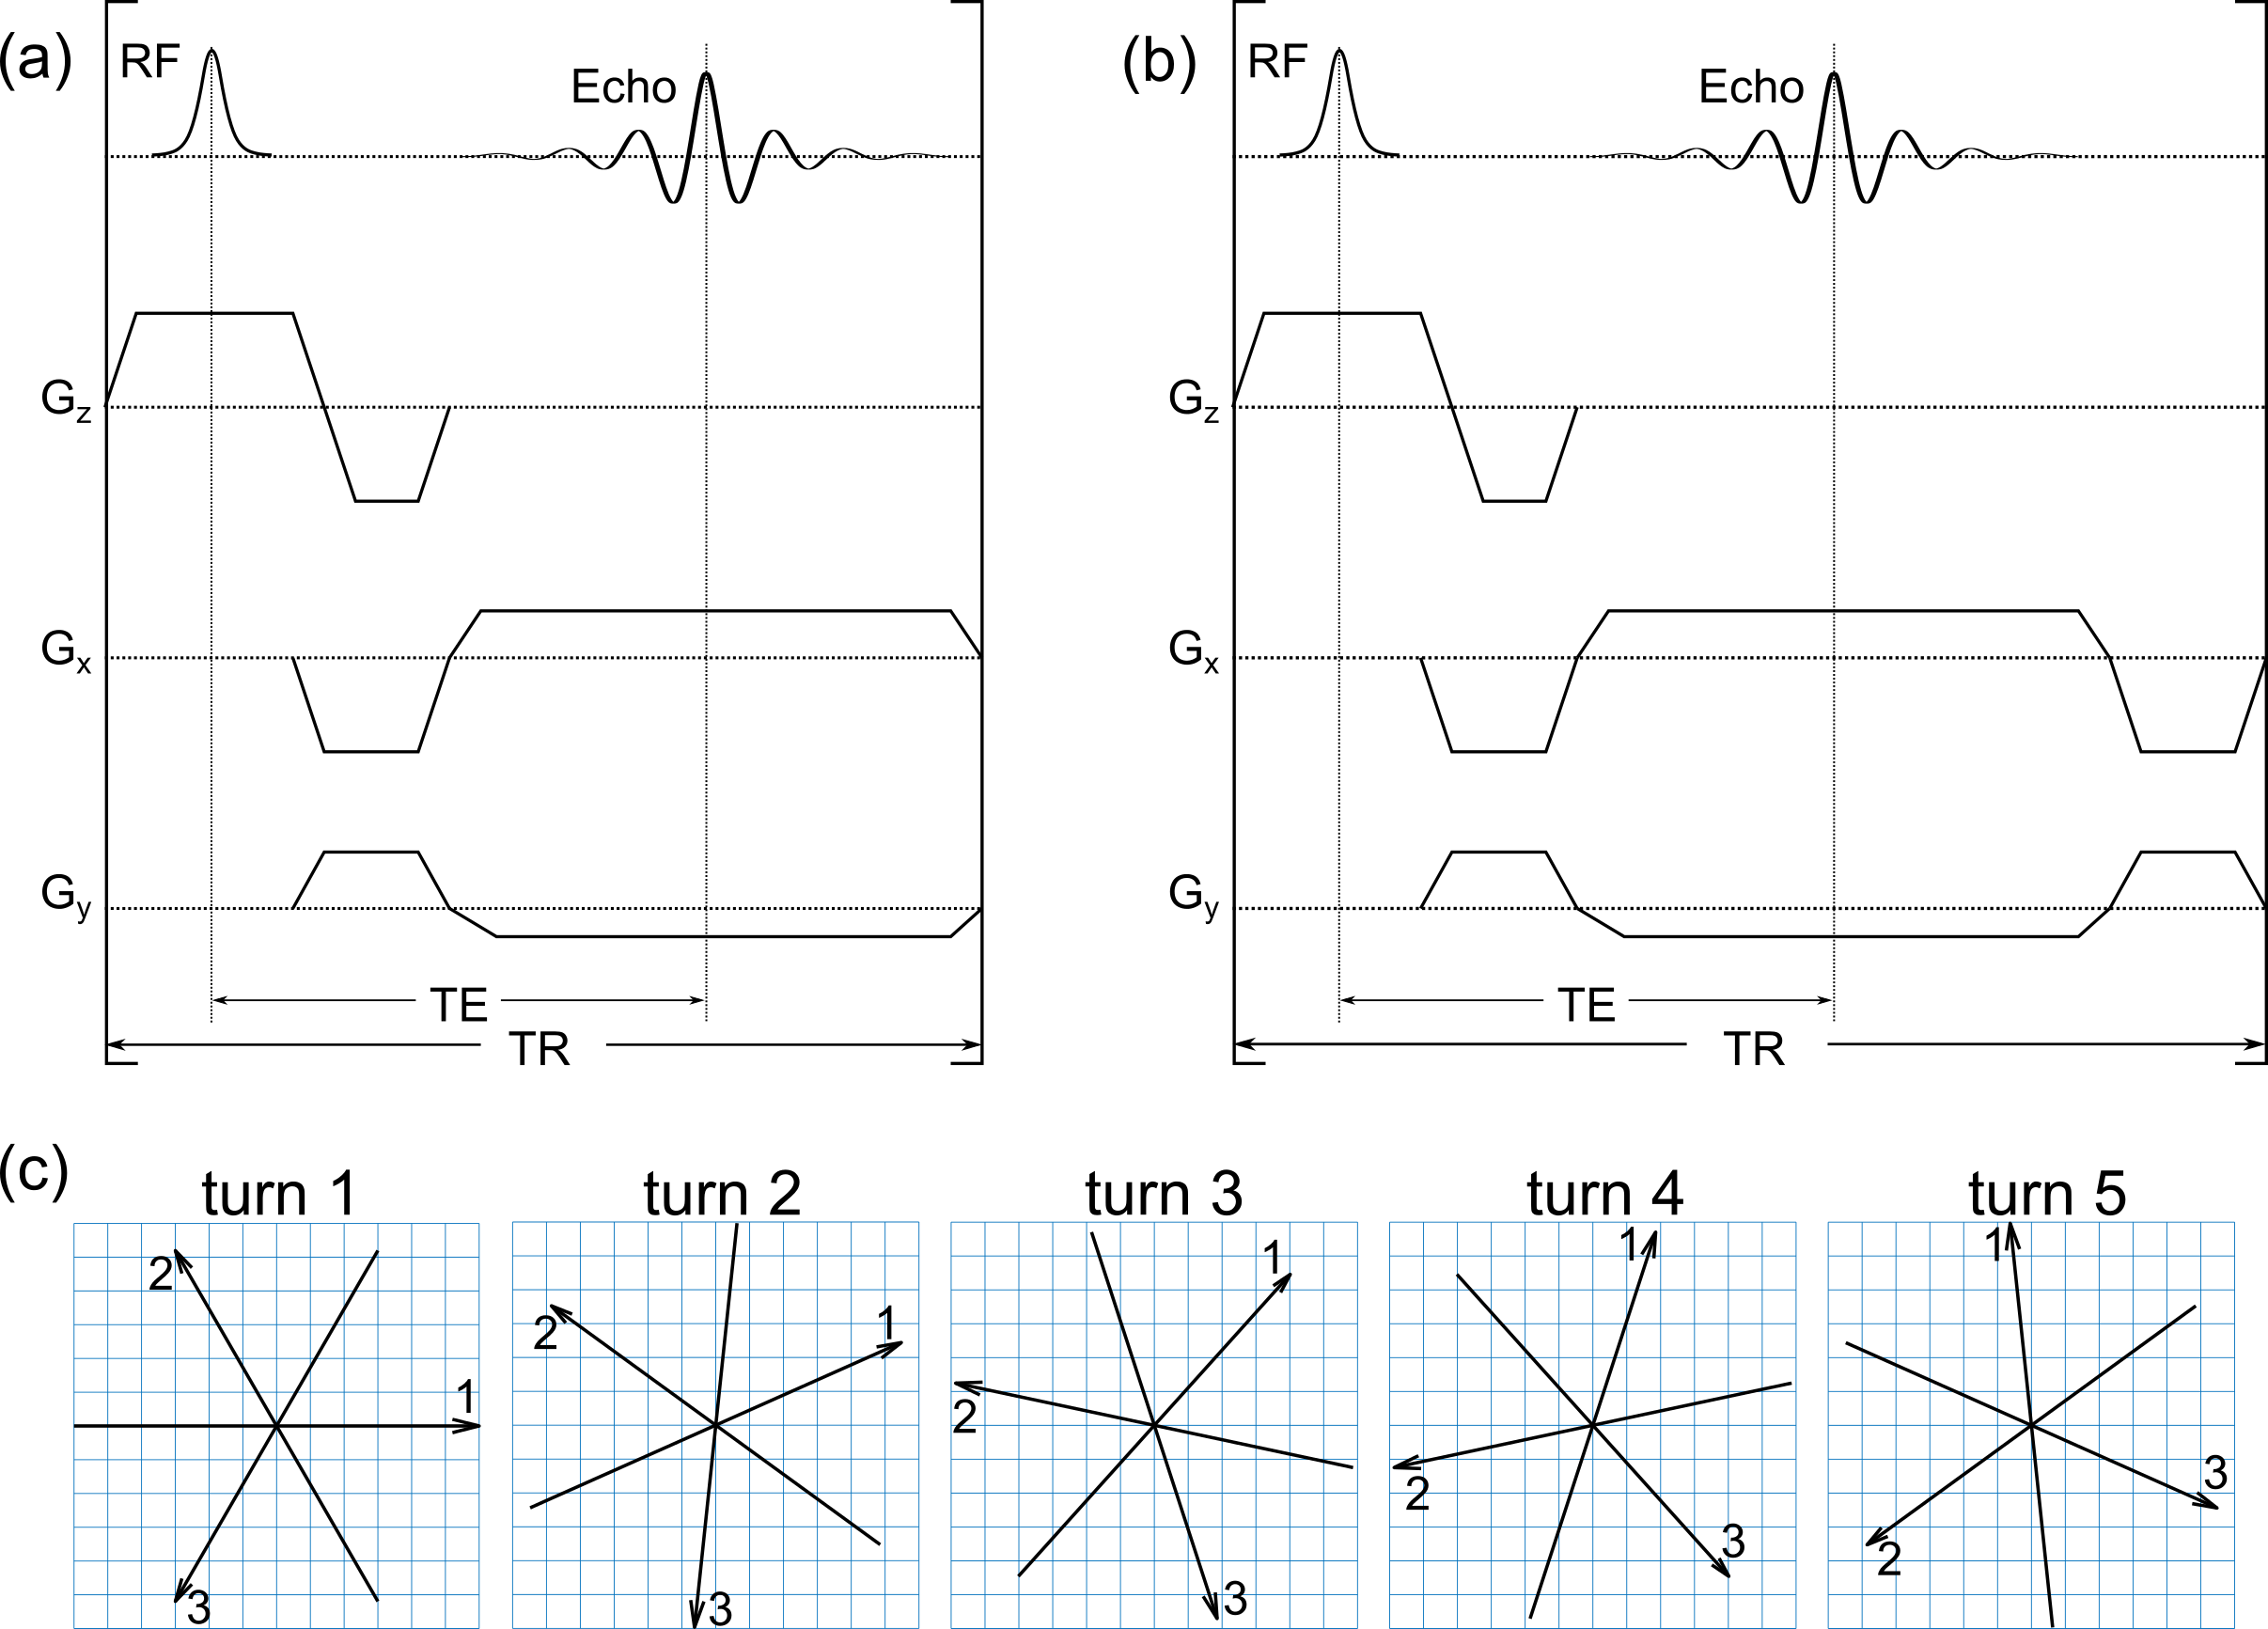
\includegraphics[width = 1.0\textwidth]{fig/rtmri-seq-rad.png}
  \caption{Undersampled radial FLASH sequences. (a) RF-spoiled radial FLASH for $T_1$-weighted imaging. (b) Refocused radial FLASH for $T_1$/$T_2$-weighted imaging. (c) Undersampled radial sampling (3 spokes per frame) with 5 sequential turns.} \label{Fig:rtmri-seq-rad}
\end{figure}
Based on radial sampling, three types of sequences have been implemented for real-time MRI: spoiled and refocused radial FLASH, and balanced steady-state free precession (\acs{bSSFP}). Beside the standard \acs{RF}-spoiling, spoiled radial FLASH (see \cref{Fig:rtmri-seq-rad}a) requires no additional rewinder gradients on the readout axes as their gradient areas vary from \acs{TR} to TR interval. The resulting image contrast in spoiled radial FLASH with short \acs{TE} and TR and low flip angle (e.g.~\ang{8}) is $T_1$-weighted. This sequence has been applied primarily to phase-contrast flow velocity quantification, real-time speech imaging, and cardiovascular magnetic resonance (\acs{CMR}) imaging. On the contrary, refocused radial FLASH (see \cref{Fig:rtmri-seq-rad}b) renders $T_2$/$T_1$-weighted image contrast and hence has been intensively used for the diagnosis of temporomandibular joint (TMJ) dysfunctions. To achieve steady state, furthermore, refocused radial FLASH does not spoil the transverse magnetization, but requires it to be consistent among TR intervals, and thus rewinder gradient is employed on both the two readout gradients. Another conventional and appealing CMR imaging sequence is \acs{bSSFP}, which offers $T_2$/$T_1$-weighted image contrast as well. bSSFP requires zero gradient area on all gradient axes, so it has an additional rewinder gradient on the slice selection gradient when compared to refocused radial FLASH. Nevertheless, bSSFP provides excellent contrast between myocardium (heart muscle) and flowing blood as myocardium has a lower $T_2$/$T_1$ ratio compared to blood. The application of bSSFP to real-time CMR imaging at \SI{1.5}{\tesla} with an achievable temporal resolution of \SI{40}{\ms} has been developed by Voit et al.~in 2013 \cite{2013_SSFP_Voit}. One drawback of bSSFP, however, is that it is prone to banding artifacts due to the off-resonance phase modulation. 

As shown in \cref{Fig:rtmri-seq-rad}c, one image frame (\textit{turn}) comprises a certain number of spokes (e.g.~$N_S = 3$), which are uniformly distributed in k-space and sequentially rotated between successive turns. Moreover, the radial sampling pattern is repeated every $N_T$ turns (e.g.~$N_T = 5$). In the current implementation of real-time MRI sequences, both $N_S$ and $N_T$ are limited to odd integers as a consequence of the total radial angle coverage set to be $2\pi$. The angle increment between two successive spokes ($\Delta \theta_{\text{spoke}}$) and that between two successive turns ($\Delta \theta_{\text{turn}}$) can be given as 
\begin{align}
  \Delta \theta_{\text{spoke}} &= 2\pi / N_S \\
\intertext{and}
  \Delta \theta_{\text{turn}}  &= 2\pi / (N_S \cdot N_T) \quad ,\\
\intertext{respectively. Therefore, the angle of the $s^{\text{th}}$ spoke in the $m^{\text{th}}$ frame is}
  \theta (s, m) &= [ (m-1) \mod{N_T} ] \cdot \Delta \theta_{\text{turn}} + (s-1) \cdot \Delta \theta_{\text{spoke}} \quad . \label{Equ:rtmri-spk-ang}
\end{align}

\section{Parallel Imaging as Nonlinear Inverse Problem} \label{Sec:rtmri-nlinv}
Prior to the nonlinear inversion (\acs{NLINV}) reconstruction for parallel imaging \cite{2007_IRGNM_PI,2008_NLINV,2010_NLINV_Heart,2010_20ms_Uecker}, joint sensitivity encoding (\acs{JSENSE}) \cite{2007_JSENSE} had been proposed by Ying et al.~in 2007 to ``jointly" estimate image content and coil sensitivity maps. However, JSENSE updates the estimate image and coil sensitivity maps in an alternative manner -- the image is estimated via CG-SENSE with the current estimate coil sensitivity maps fixed, and then coil sensitivity maps are estimated via the CG-type method with the current estimate image fixed. In short, this method separates a nonlinear inverse problem into two linear inverse problems and solve them alternatively. NLINV is the first algorithm that jointly estimates image content and coil sensitivity maps via the iteratively regularized Gauss-Newton method (\acs{IRGNM}) \cite{1996_regu_inv,2004_iter_inv}. 

\subsection*{Algorithm}
Following \cref{Equ:mri-pi-forward}, the system equation in parallel imaging can be written as
\begin{equation} \label{Equ:rtmri-nlinv-system}
  y = F(x) \quad \text{with} \; x = 
  \left( \begin{array} {c}
    \rho \\
    c_1 \\
    \vdots \\
    c_N \\
  \end{array} \right)
\end{equation}
with both the image ($\rho$) and coil sensitivity maps being the unknown ($x$). Here, it is convenient to denote the forward operation on the $n$\textsuperscript{th} coil as $F_n (x) = P \mathcal{F} \{ \rho \cdot c_n \}$.

\cref{Equ:rtmri-nlinv-system} represents a \textit{nonlinear} system because when assuming $x_1 = (\rho_1,~c_1)^T$ and $x_2 = (\rho_2,~c_2)^T$, a linear system satisfies $F(x_1) + F(x_2) = F(x_1 + x_2)$, but 
\begin{align*}
  F(x_1) + F(x_2) 
  &= P \mathcal{F} \{ \rho_1 \cdot c_1 \} + P \mathcal{F} \{ \rho_2 \cdot c_2 \} \\
  &= P \mathcal{F} \{ \rho_1 \cdot c_1 + \rho_2 \cdot c_2 \} \quad , \\
\intertext{which is not equal to} 
  F(x_1 + x_2) 
  &= F \begin{pmatrix}
    \rho_1 + \rho_2 \\
    c_1 + c_2
  \end{pmatrix} \\
  &= P \mathcal{F} \{ (\rho_1 + \rho_2) \cdot (c_1 + c_2) \} \quad .
\end{align*} 
To solve this nonlinear problem, IRGNM firstly linearizes it as $y = DF(x_n) \text{d}x + F(x_n)$, where $x_n$ is the estimate from $n^{\text{th}}$ Newton step and $DF(x_n)$ is the Frech\'et derivative. Thus, the cost function in \cref{Equ:mri_inv_cost} becomes 
\begin{equation} \label{Equ:rtmri-nlinv-cost}
  \Phi(\text{d}x) = \argmin\limits_{\text{d}x} \norm{DF(x_n)\text{d}x - [y - F(x_n)]}_2^2 + \alpha_n \norm{W ( x_n + \text{d}x - x_0 )}_2^2
\end{equation}
with $\alpha_n$ being the Tikhonov regularization parameter, $x_0$ the initial guess, which is initialized by the estimate from the preceding frame damped by a dampening factor $p$ ($0 \leq p \leq 1$). To counteract the ill-condition of this inverse problem, the unknown $x$ is subject to a transformation by the preconditioning matrix $W$, 
\begin{equation} \label{Equ:rtmri-nlinv-W}
  \hat{x} = 
  \left( \begin{array}{c}
    \rho \\
    \hat{c}_1 \\
    \vdots \\
    \hat{c}_N \\
  \end{array} \right) = 
  \begin{pmatrix}
    I &                                             &        & \\
      & \Big( 1 + s \norm{\vec{k}}_2^2 \Big)^{-l} \mathcal{F} &        & \\
      &                                             & \ddots & \\
      &                                             &        & \Big( 1 + s \norm{\vec{k}}_2^2 \Big)^{-l} \mathcal{F}
  \end{pmatrix} 
  \left( \begin{array}{c}
    \rho \\
    c_1 \\
    \vdots \\
    c_N \\
  \end{array} \right)
\end{equation}
with $\vec{k}$ being 2D Cartesian grid, $s = 440$, and $l = 16$. This transformation ensures the spatial smoothness of coil sensitivity maps, as the signal from high spatial frequency region is strongly penalized. With this preconditioning, the cost function can be solved via conjugate gradient method with Tikhonov regularization. The optimized $\text{d}x$ is then used to update $x_{n+1}$: $x_{n+1} = x_n + \text{d}x$. Beside the forward operator $F(x)$, the solution of \cref{Equ:rtmri-nlinv-cost} requires $DF(x)$ and its adjoint $DF^{H} (x)$. A fast forward computation of $DF(x)$ can be derived via the Jacobian matrix
\begin{align}
  DF(x) \begin{pmatrix}
    \text{d} \rho \\
    \text{d} c_1 \\
    \vdots \\
    \text{d} c_N
  \end{pmatrix} 
  &= \begin{pmatrix}
    \frac{\partial}{\partial \rho} F_1 (x) & \frac{\partial}{\partial c_1} F_1 (x) & \cdots & \frac{\partial}{\partial c_N} F_1 (x) \\
    \frac{\partial}{\partial \rho} F_2 (x) & \frac{\partial}{\partial c_1} F_2 (x) & \cdots & \frac{\partial}{\partial c_N} F_2 (x) \\
    \vdots & \vdots & \ddots & \vdots \\
    \frac{\partial}{\partial \rho} F_N (x) & \frac{\partial}{\partial c_1} F_N (x) & \cdots & \frac{\partial}{\partial c_N} F_N (x) 
  \end{pmatrix} \begin{pmatrix}
    \text{d} \rho \\
    \text{d} c_1 \\
    \vdots \\
    \text{d} c_N
  \end{pmatrix} \nonumber \\
  &= \begin{pmatrix}
    P\mathcal{F}c_1 & P\mathcal{F}\rho & 0                & \cdots & 0 \\
    P\mathcal{F}c_2 & 0                & P\mathcal{F}\rho & \cdots & 0 \\
    \vdots          & \vdots           & \vdots           & \ddots & \vdots \\
    P\mathcal{F}c_N & 0                & 0                & \cdots & P\mathcal{F}\rho
  \end{pmatrix} \begin{pmatrix}
    \text{d} \rho \\
    \text{d} c_1 \\
    \vdots \\
    \text{d} c_N
  \end{pmatrix} \nonumber \\
  &= \begin{pmatrix}
    P\mathcal{F} \{ c_1 \cdot \text{d}\rho + \rho \cdot \text{d} c_1 \} \\
    \vdots \\
    P\mathcal{F} \{ c_N \cdot \text{d}\rho + \rho \cdot \text{d} c_N \} 
  \end{pmatrix} \quad . \label{Equ:rtmri-nlinv-der} 
\end{align}
$DF^{H} (x)$ can then be exploited by taking the conjugate transpose of $DF(x)$
\begin{align}
  DF^{H} (x) \begin{pmatrix}
    \text{d} y_1 \\
    \vdots \\
    \text{d} y_N
  \end{pmatrix}
  &= \begin{pmatrix}
    c_1^* \mathcal{F}^{-1} P^H & c_2^* \mathcal{F}^{-1} P^H & \cdots & c_N^* \mathcal{F}^{-1} P^H \\
    \rho^* \mathcal{F}^{-1} P^H & 0 & \cdots & 0 \\
    0 & \rho^* \mathcal{F}^{-1} P^H & \cdots & 0 \\
    \vdots & \vdots & \ddots & \vdots \\
    0 & 0 & \cdots & \rho^* \mathcal{F}^{-1} P^H
  \end{pmatrix} \begin{pmatrix}
    \text{d} y_1 \\
    \vdots \\
    \text{d} y_N
  \end{pmatrix} \nonumber \\
  &= \begin{pmatrix}
    \sum_{n=1}^{N} c_n^* \cdot \mathcal{F}^{-1} P^H \text{d} y_n \\
    \rho^* \cdot \mathcal{F}^{-1} P^H \text{d} y_1 \\
    \vdots \\
    \rho^* \cdot \mathcal{F}^{-1} P^H \text{d} y_N 
  \end{pmatrix} \quad . \label{Equ:rtmri-nlinv-adj}
\end{align}
With these two operators, the update rule of $\text{d}x$ can be derived from \cref{Equ:rtmri-nlinv-cost}
\begin{equation} \label{Equ:rtmri-dx-sol}
  \text{d}x = [DF(x_n)^H DF(x_n) + \alpha_n I]^{-1} \{ DF(x_n)^H [y-F(x_n)] + \alpha_n (x_0 - x_n) \}
\end{equation}

For the reconstruction of serial images via real-time MRI acquisitions, the algorithm is initialized with $\rho=1$ and $c_n = 0$ for the first frame, while the following frames are initialized with the estimate from the preceding frame, which effectively acts as temporal regularizations. The incorporation of the temporal regularization into NLINV enforces temporal correlations among successive image frames. The regularization parameter decays along Newton steps according to $\alpha_n = \alpha_0 \cdot 2^{-n}$ and $\alpha_0 = 1$.

As the iterative NLINV image reconstruction technique is of heavy computational load and time consuming, it has been implemented on multiple graphics processing units (\acsp{GPU}) and fully integrated into the reconstruction pipeline of the MRI system \cite{2012_Schaetz}. 

\subsection*{Preprocessing}
Before NLINV image reconstructions, the acquired multi-channel k-space data is firstly corrected for gradient delays \cite{2011_GDC}, then compressed to \num{10} virtual channels via principle component analysis, and finally gridded onto 2D Cartesian grids without density compensation and normalized to \num{100} in the $L^2$ norm. On the other hand, the sampling pattern $P$ (refer to \cref{Equ:mri-pi-forward}) is the projection onto the measured k-space positions.

\subsection*{Postprocessing}
A temporal median filter with a window size equivalent to the number of turns can be applied to the reconstructed images. Furthermore, a modified version of the non-local means denoising \cite{2005_NLM} algorithm has been developed and integrated into the online reconstruction pipeline by Klosowski et al.~\cite{2016_NLM}. 


\section{Real-Time Phase-Contrast Flow MRI} \label{Sec:rtmri-pc}

\subsection{Physical Principles}
Real-time phase-contrast flow MRI has been an important technique as it provides quantitative information for the evaluation of cardiovascular diseases. Phase-contrast flow MRI is based on the discovery by Hahn in 1960 \cite{1960_PC_Hahn} which states that velocities of flowing spins can be encoded into the phase via a bipolar gradient, under which the temporal evolution of phases can be mathematically expressed as 
\begin{align} 
  \phi(t) &= \gamma \int_{0}^{T} G(t) x(t) \text{d} t \nonumber \\
          &= \gamma \int_{0}^{T} G(t) (x_0 + v_0 t + \frac{1}{2} a_0 t^2 + \cdots ) \text{d} t \quad \text{(Taylor Series)} \nonumber \\
          &= \gamma x_0 \int_{0}^{T} G(t) \text{d} t + \gamma v_0 \int_{0}^{T} G(t) t \text{d} t + \cdots \label{Equ:rtmri-pc-math}
\end{align}
the first two integrals of which represent the phase for the static spins at location $x_0$ without macroscopic movements and the flowing spins with a constant moving velocity $v_0$, respectively. According to this equation, both spins have zero phase by the end of the flow-compensation (also named velocity-compensation) gradient ($G_{\text{FC}}$) with the waveform $1 \bar{2} 1$, as depicted in the left part of \cref{Fig:rtmri-pc-theory}. With the velocity-encoding (also named flow-encoding) gradient ($G_{\text{VENC}}$) with the waveform $1 \bar{1}$, however, the static spins still result in zero phase and the flowing spins with constant velocity have a net phase, 
\begin{align} 
  \phi_v (2\tau) &= \gamma v_0 \int_{0}^{2\tau} G(t) t \text{d} t \nonumber \\
                 &= \gamma G_0 v_0 \left( \int_{0}^{\tau} t \text{d} t - \int_{\tau}^{2\tau} t \text{d} t \right) \nonumber \\
                 &= - \gamma G_0 \tau^2 v_0 \label{Equ:rtmri-pc-vel}
\end{align}
which indicates that the velocity is linearly proportional to the accumulated net phase, as depicted in right part of \cref{Fig:rtmri-pc-theory}. Therefore, the velocity-encoding (\acs{VENC}) range, determined by the velocity-encoding gradient amplitude ($G_0$) and duration ($\tau$) has to be larger than the velocity to be measured ($v$). Otherwise, the image area with exceeded velocities incurs velocity \textit{aliasing} artifacts, appearing as random phase values. However, VENC can not be arbitrarily large because the SNR of the measured phase is constrained by the VENC \cite{1991_PD_CD_PC}
\begin{equation}
  \snr_{\phi_v} \propto \snr_{\text{Mag}} \cdot \frac{\abs{v}}{\text{VENC}}
\end{equation}
with $\snr_{\text{Mag}}$ being the SNR of the measured magnitude image. Thus, imaging protocols may require several measurements until the peak velocity is free of aliasing.

\begin{figure}[tb]
  \centering
  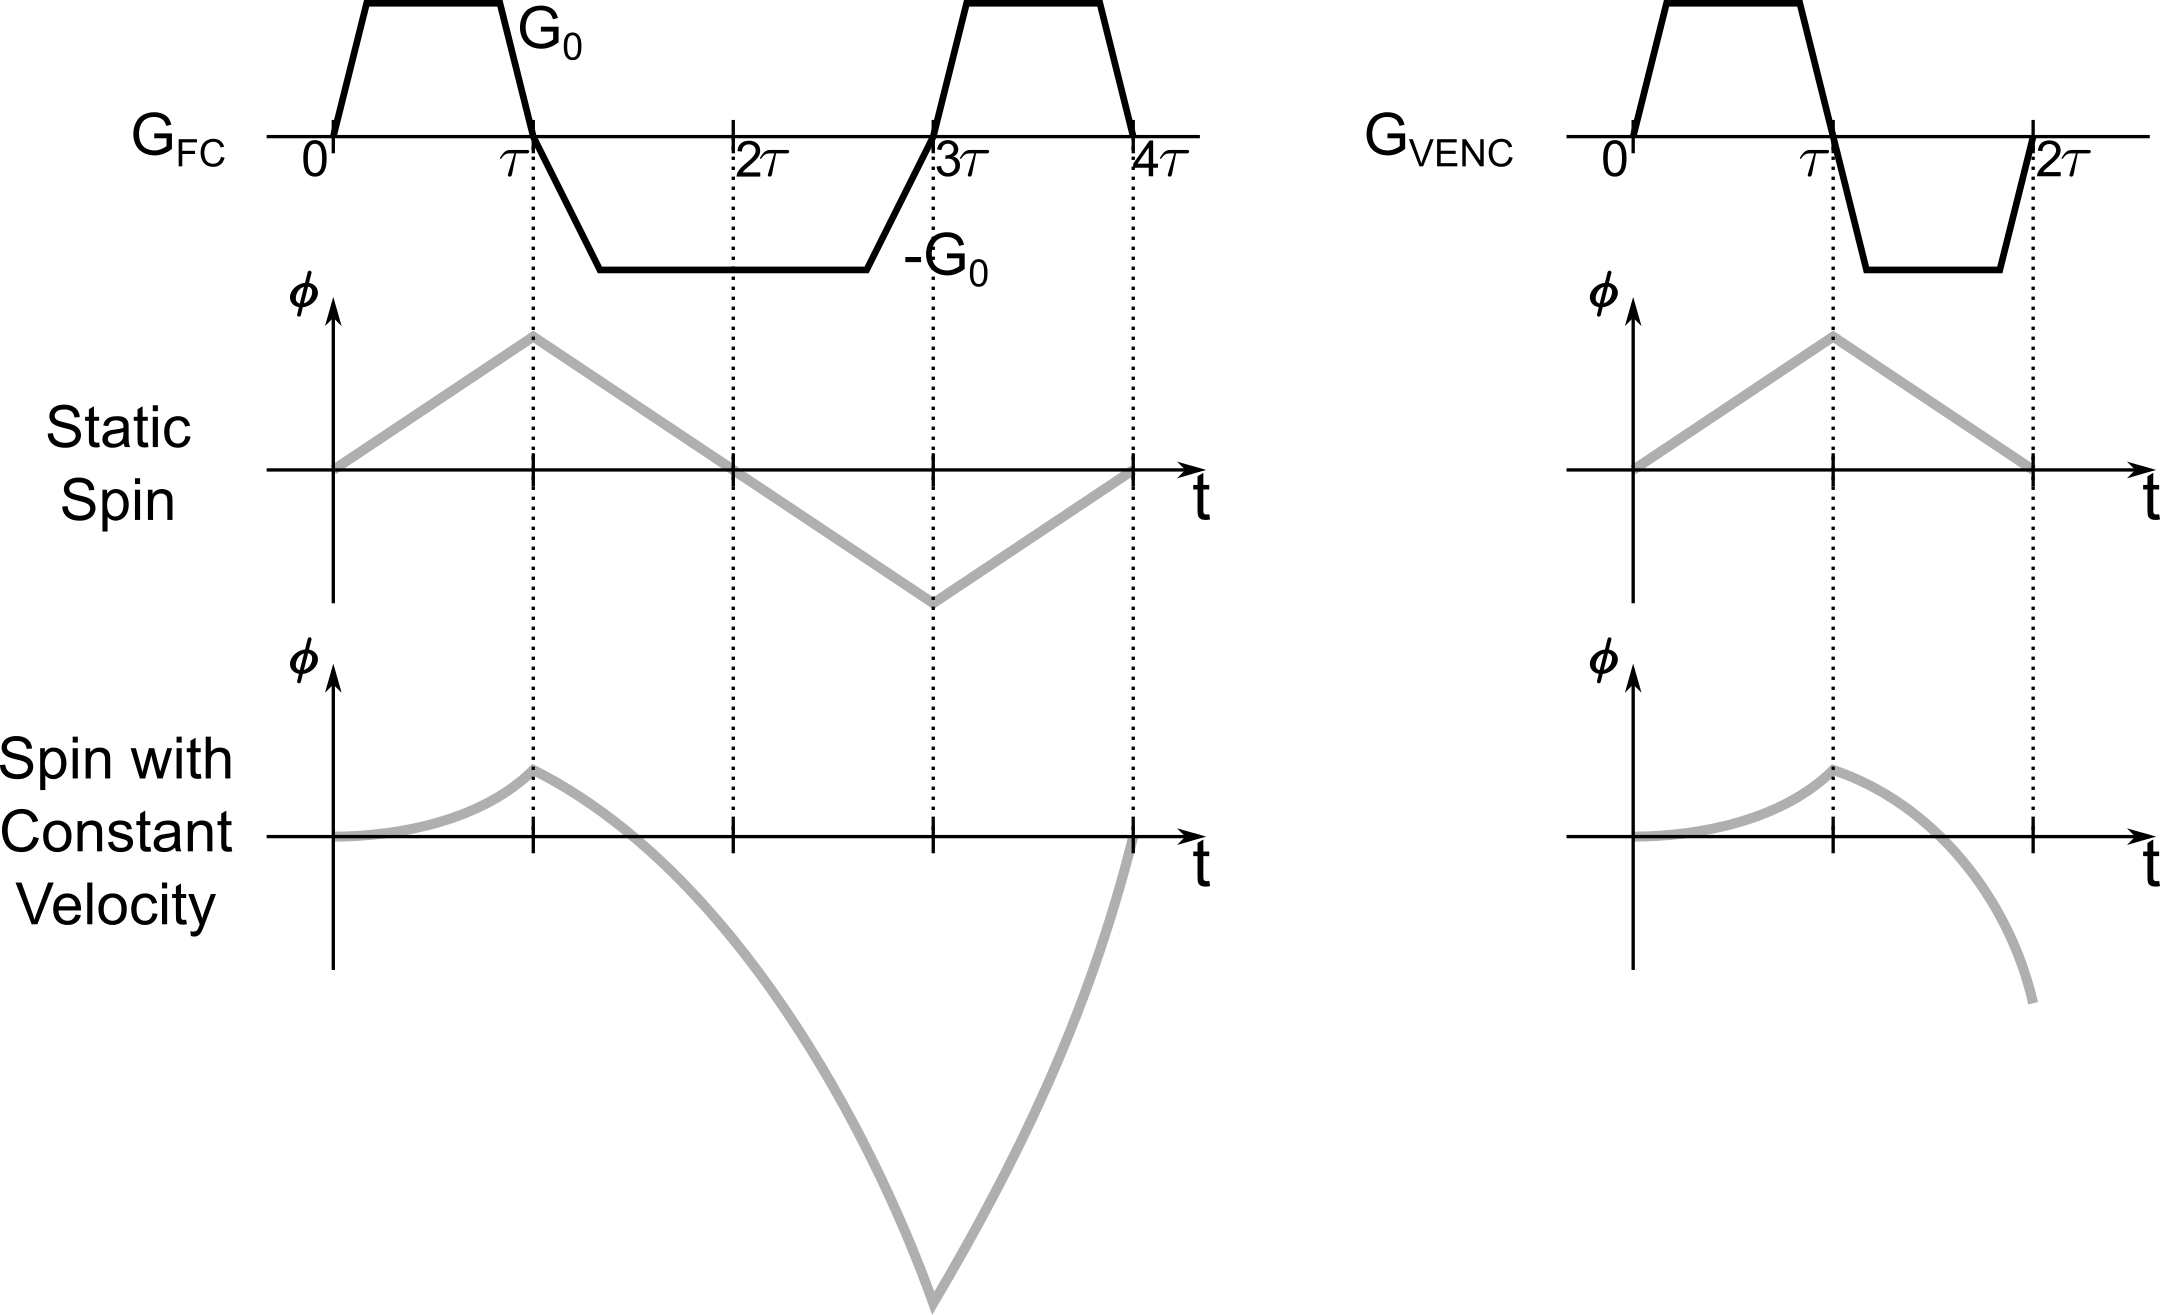
\includegraphics[width = 1.0\textwidth]{fig/rtmri-pc-theory.png}
  \caption{Schematic illustrations of flow compensation and velocity encoding. (Left) Flow-compensation (FC) gradient with the waveform $1 \bar{2} 1$ results in zero phase for both the static spin and the spin with constant velocity. (Right) Velocity-encoding (\acs{VENC}) gradient with the waveform $1 \bar{1}$ results in zero phase for the static spin but net phase for the spin with constant velocity.} \label{Fig:rtmri-pc-theory}
\end{figure}

MR image phase, however, can have various sources, e.g.~the off-resonance-induced phase modulation. Therefore, to remove unwanted phases, at least two measurements with different velocity encodings are needed to obtain quantitative velocities. This can be implemented in two manners. The first approach is typically named two-sided velocity encoding \cite{2012_PC_SVE}, where the first measurement consists of a bipolar (e.g.~positive and negative) velocity-encoding gradient and the second one uses a velocity-encoding gradient with signs reversed. As a result, the phase difference between the two-sided measurements is $\Delta \phi = 2 \gamma G_0 \tau^2 v_0$. The second approach is named one-sided velocity encoding \cite{2012_PC_SVE}, where the first measurement employs the flow-compensation gradient to zero phases caused by motions and the second one uses the bipolar velocity-encoding gradient, and hence the phase difference between the one-sided measurements is $\Delta \phi = - \gamma G_0 \tau^2 v_0$. In principle, flow-encoding gradients can be applied in any direction to encode multi-dimensional velocities.

\subsection{Image Reconstructions}
In the current implementation of the real-time phase-contrast flow MRI sequence, only through-plane velocities are encoded via the one-sided velocity encoding, consisting of one flow-compensation and one flow-encoding acquisition. The two datasets are treated as two independent streams and separately reconstructed by NLINV except that they share the same channel compression matrix in the preprocessing process. The reconstructed image and coil sensitivity maps are combined to remove unwanted phase contributions from coils,
\begin{equation} \label{Equ:rtmri-pc-rho-coil}
  \rho_{j,l} = \frac{\rho_l \cdot c_{j,l}}{\sqrt{\sum_{j} c_{j,l} \cdot c^{*}_{j,l}}} \quad \text{with} \; j \in [1,N], \; l \in [1,2]
\end{equation}
with $j$ and $l$ being the index of coils and acquisitions respectively, and $*$ the complex conjugate. Thus, the complex phase-contrast map can be calculated via
\begin{align}
  \hat{\rho}_{\text{PC}} &= \sum_{j} \rho_{j,0} \cdot \rho^{*}_{j,1} \\
  \rho_{\text{PC}} &= \frac{\hat{\rho}_{\text{PC}}}{\sqrt{|\hat{\rho}_{\text{PC}}|}} \quad .
\end{align}

For quantitative flow evaluations, the complex phase-contrast maps are imported into CAIPI prototype software (Fraunhofer MEVIS\footnote{\url{http://www.mevis.fraunhofer.de/}}, Bremen, Germany), where two subsets of images are available, one anatomical magnitude image and one phase-difference (e.g.~velocity) map. To begin with, a region-of-interest (\acs{ROI}) in a certain magnitude image frame is manually selected, i.e., the ascending aorta lumen, which is then propagated through the entire image series. The propagation is able to capture the moving lumen. If not properly captured, manual corrections can be done afterwards. With the lumen determined from every phase-contrast map, CAIPI then calculates a list of flow parameters, e.g.~peak velocity, flow per heartbeat, flow volume, and regurgitation fraction.




\chapter{Numerical Simulations} \label{Chp:sim}
\chaptermark{Numerical Simulations}

Numerical simulation has been an important tool in \acs{MRI} because unexpected errors due to system imperfections (e.g.~eddy currents, noise, and field inhomogeneities) and uncooperative patients (e.g.~through-plane motions) can be excluded. Moreover, it creates an ideal imaging environment that fosters understanding the characteristics of different k-space sampling trajectories and evaluating reconstruction methods. Therefore, a simulation framework based on analytical Fourier transformation is built for the studies of various radial sampling schemes, e.g.~asymmetric-echo and multi-echo radial \acs{FLASH}.

\section{Fundamentals}
In principle, the MR signal in k-space is the continuous Fourier transform of the scanned object $\rho(\vec{r})$, which can be written as 
\begin{equation} \label{Equ:cont_FT_rho}
y(t) = \int_{\vec{r}} \rho(\vec{r}) \cdot e^{-i 2\pi \cdot \vec{k}(t) \cdot \vec{r}} \text{d} \vec{r}
\end{equation}

One typical MR simulation was based on rasterized phantoms, and the MR signal was obtained via discrete Fourier transform (\acs{DFT}). This approach, however, is time consuming as every k-space signal requires an execution of DFT over all image pixels. Nevertheless, it leads to the inverse-crime problem, as the same discrete model of the imaging system is used for both simulation and image reconstruction. Moreover, the MR signal from a rasterized phantom can not represent the aliasing artifact from truncated k-space. Therefore, it is more reliable and preferable to use analytical phantoms with three important features.

First of all, the analytical Fourier transform of phantoms constructed by superimposed ellipses and rectangles (e.g.~Shepp-Logan phantom \cite{1974_SL,2008_SL_Gach}) can be derived as
\begin{align} 
  A_{\text{circ}}(k_x,k_y) &= a \cdot b \cdot \frac{J_1(\sqrt{(a \cdot k_x)^2 + (b \cdot k_y)^2})}{\sqrt{(a \cdot k_x)^2 + (b \cdot k_y)^2}} \label{Equ:aFT_circ} \\
\intertext{and}
  A_{\text{rect}}(k_x,k_y) &= 2\pi \cdot a \cdot b \cdot \sinc(a \cdot k_x) \cdot \sinc(b \cdot k_y) \label{Equ:aFT_rect}
\end{align}
respectively \cite{2008_Block_Thesis}. Here, $J_1(x)$ is the first-order Bessel function of its first kind, $a$ and $b$ represent either the short and long axes of an ellipse, or the length and width of a rectangle. On the other hand, due to the linearity of Fourier transform, superimpositions in image domain are equivalent to those in k-space. Therefore, the analytical Fourier transform of any phantom with superimposed ellipses and/or rectangles can be calculated given the sampling k-space trajectory, which is given as
\begin{equation} \label{Equ:sum_aFT_rho}
  y(\vec{k}) = \sum_{m} I_m \cdot A_m(\vec{k})
\end{equation}
with $m$ being the index for ellipses and rectangles in the phantom, and $I_m$ and $A_m$ the corresponding proton density and analytical Fourier transform, respectively.

Secondly, the inclusion of multiple spatially-varying receiver coils $c_j(\vec{x})$ to mimic parallel imaging, which extends the MR signal in \cref{Equ:cont_FT_rho} to 
\begin{equation} \label{Equ:cont_FT_rho_coil}
  y_j(t) = \int_{\vec{r}} c_j(\vec{r}) \cdot \rho(\vec{r}) \cdot e^{-i 2\pi \cdot \vec{k}(t) \cdot \vec{r}} \text{d} \vec{r} \quad .
\end{equation}
With sinusoidal or polynomial fitting of the complex coil sensitivity map simulated from Biot-Savart law, the fitting coefficients can be integrated into the analytical Fourier transform of phantoms. Mathematical description of the integration procedure is given in \cref{Chp:AnalCoil}.

Thirdly, the inclusion of relaxation effects (e.g.~\acs{T2s} signal decay and off-resonance phase modulation in multi-echo FLASH) into the MR signal model, which is further extended from \cref{Equ:cont_FT_rho_coil} to
\begin{equation} \label{Equ:cont_FT_rho_coil_ME}
  y_{j,l}(t) = \int_{\vec{r}} c_j(\vec{r}) \cdot \rho(\vec{r}) \cdot e^{-[R_2^*(\vec{r}) + i 2\pi \cdot \Delta f (\vec{r})] \cdot \text{TE}_l} \cdot e^{-i 2\pi \cdot \vec{k}(t) \cdot \vec{r}} \text{d} \vec{r}
\end{equation}
where $R_2^*$ is the reciprocal of the $T_2^*$ relaxation time, $\Delta f$ is the off-resonance frequency map, and $\text{TE}_l$ is the echo time of the $l$\textsuperscript{th} echo. The relaxation effects can be included by assuming $T_2^*$ and $\Delta f$ values in every shape (ellipse or rectangle) to be constant, so that the MR signal in accordance to \cref{Equ:sum_aFT_rho} is (ignoring the coil sensitivities for simplicity)
\begin{equation} \label{Equ:sum_aFT_rho_relax}
  y_l(\vec{k}) = \sum_{m} I_m \cdot e^{-z_m \cdot \text{TE}_l} \cdot A_m(\vec{k})
\end{equation}
with $z_m = R_2^* + i 2\pi \cdot \Delta f$. One drawback of this method is that off-resonances are constant within a shape and hence discrete in a phantom, which does not reflect the fact that off-resonance frequency maps are usually smooth and slowly-varying in space, similar to coil sensitivity maps. This drawback, however, can be overcome using approximation methods as for coils.

Using the analytical phantom with the above features, a numerical simulation framework was developed in MATLAB (Mathworks, Natick, MA, IUSA) for studying the characteristics of different radial sampling schemes.

\section{In-Plane Motion Simulations}
To study motion artifacts in real-time MRI, to mimic the experimental motion phantom \cite{2013_MotionPha}, and to test motion-correction algorithms (e.g.~application of k-space energy spectrum analysis to motion correction in \acs{PROPELLER} MRI \cite{2006_KESA,2012_KESA_Tan}), this simulation framework is capable of adding in-plane motions (e.g. translation and rotation) to every acquired k-space spoke. 

The principle of motion simulation is that the geometries of all shapes contained in a phantom (i.e., the center, the major and minor semi-axes of a ellipse) are consistent during the acquisition of a spoke, and thus the k-space signal of this spoke can be calculated by analytical Fourier transform given the known geometries. The geometries can then be changed for the acquisition of the next spoke. Taking in-plane rotation as an example, the centers of the two tubes are updated every spoke by rotating the tubes around the center of the imaging slice according to the user-defined rotation angle per spoke. Note that the rotation angle can be converted to the rotation speed (\si{\cm\per\second}) as used in the experimental motion phantom,
\begin{equation} \label{Equ:rot_speed}
v = \phi \cdot d / T
\end{equation}
where $\phi$ is the rotation angle per frame, $d$ the distance from the center of the tube to that of the rotation, and $T$ the acquisition time for one image. Therefore, the rotation angle of \ang{5.7} per frame in \cref{Fig:sim-motion-halfPos} corresponds to half-position shift and \SI{15}{\cm\per\second} for the outer tube. As the distance to the image center from the outer tube is twice as long as the inner one, the outer tube rotates twice as fast and hence it suffers from more severe blurring. 

Furthermore, to prove the temporal acuity of NLINV without the temporal median filter, \cref{Fig:sim-motion-comp} compares it with the conventional Gridding \& FFT reconstruction \cite{1991_conv_gridding,2005_gridding}. Firstly, as shown in the static phantom images, NLINV can greatly suppress streaking artifacts due to undersampling as it iteratively estimates the optimal image that matches best with the acquired k-space data, while Tikhonov regularization on the image penalizes unwanted signals from high-spatial-frequency area, i.e., noise and streaks. Secondly, the rotation angle per frame \ang{5.7}, \ang{11.4}, and \ang{17.1} corresponds to the rotation speed of \SI{15}{\cm\per\second}, \SI{30}{\cm\per\second} and \SI{45}{\cm\per\second} for the outer tube, respectively. The resulting images from Gridding \& FFT reconstruction are degraded by heavier spatial discontinuity along with higher rotation speed, while images from NLINV show blurring artifacts because NLINV for serial images relies on the temporal regularization, which could be explored to find an optimum for rapid-motion imaging, i.e. \SI{45}{\cm\per\second}. The optimization of the regularization parameters, however, is beyond the scope of this chapter.

In short, these simulation results match the findings from real-time MRI on the experimental motion phantom \cite{2014_Temp_Fidelity}.
\begin{figure}[tb]
  \centering
  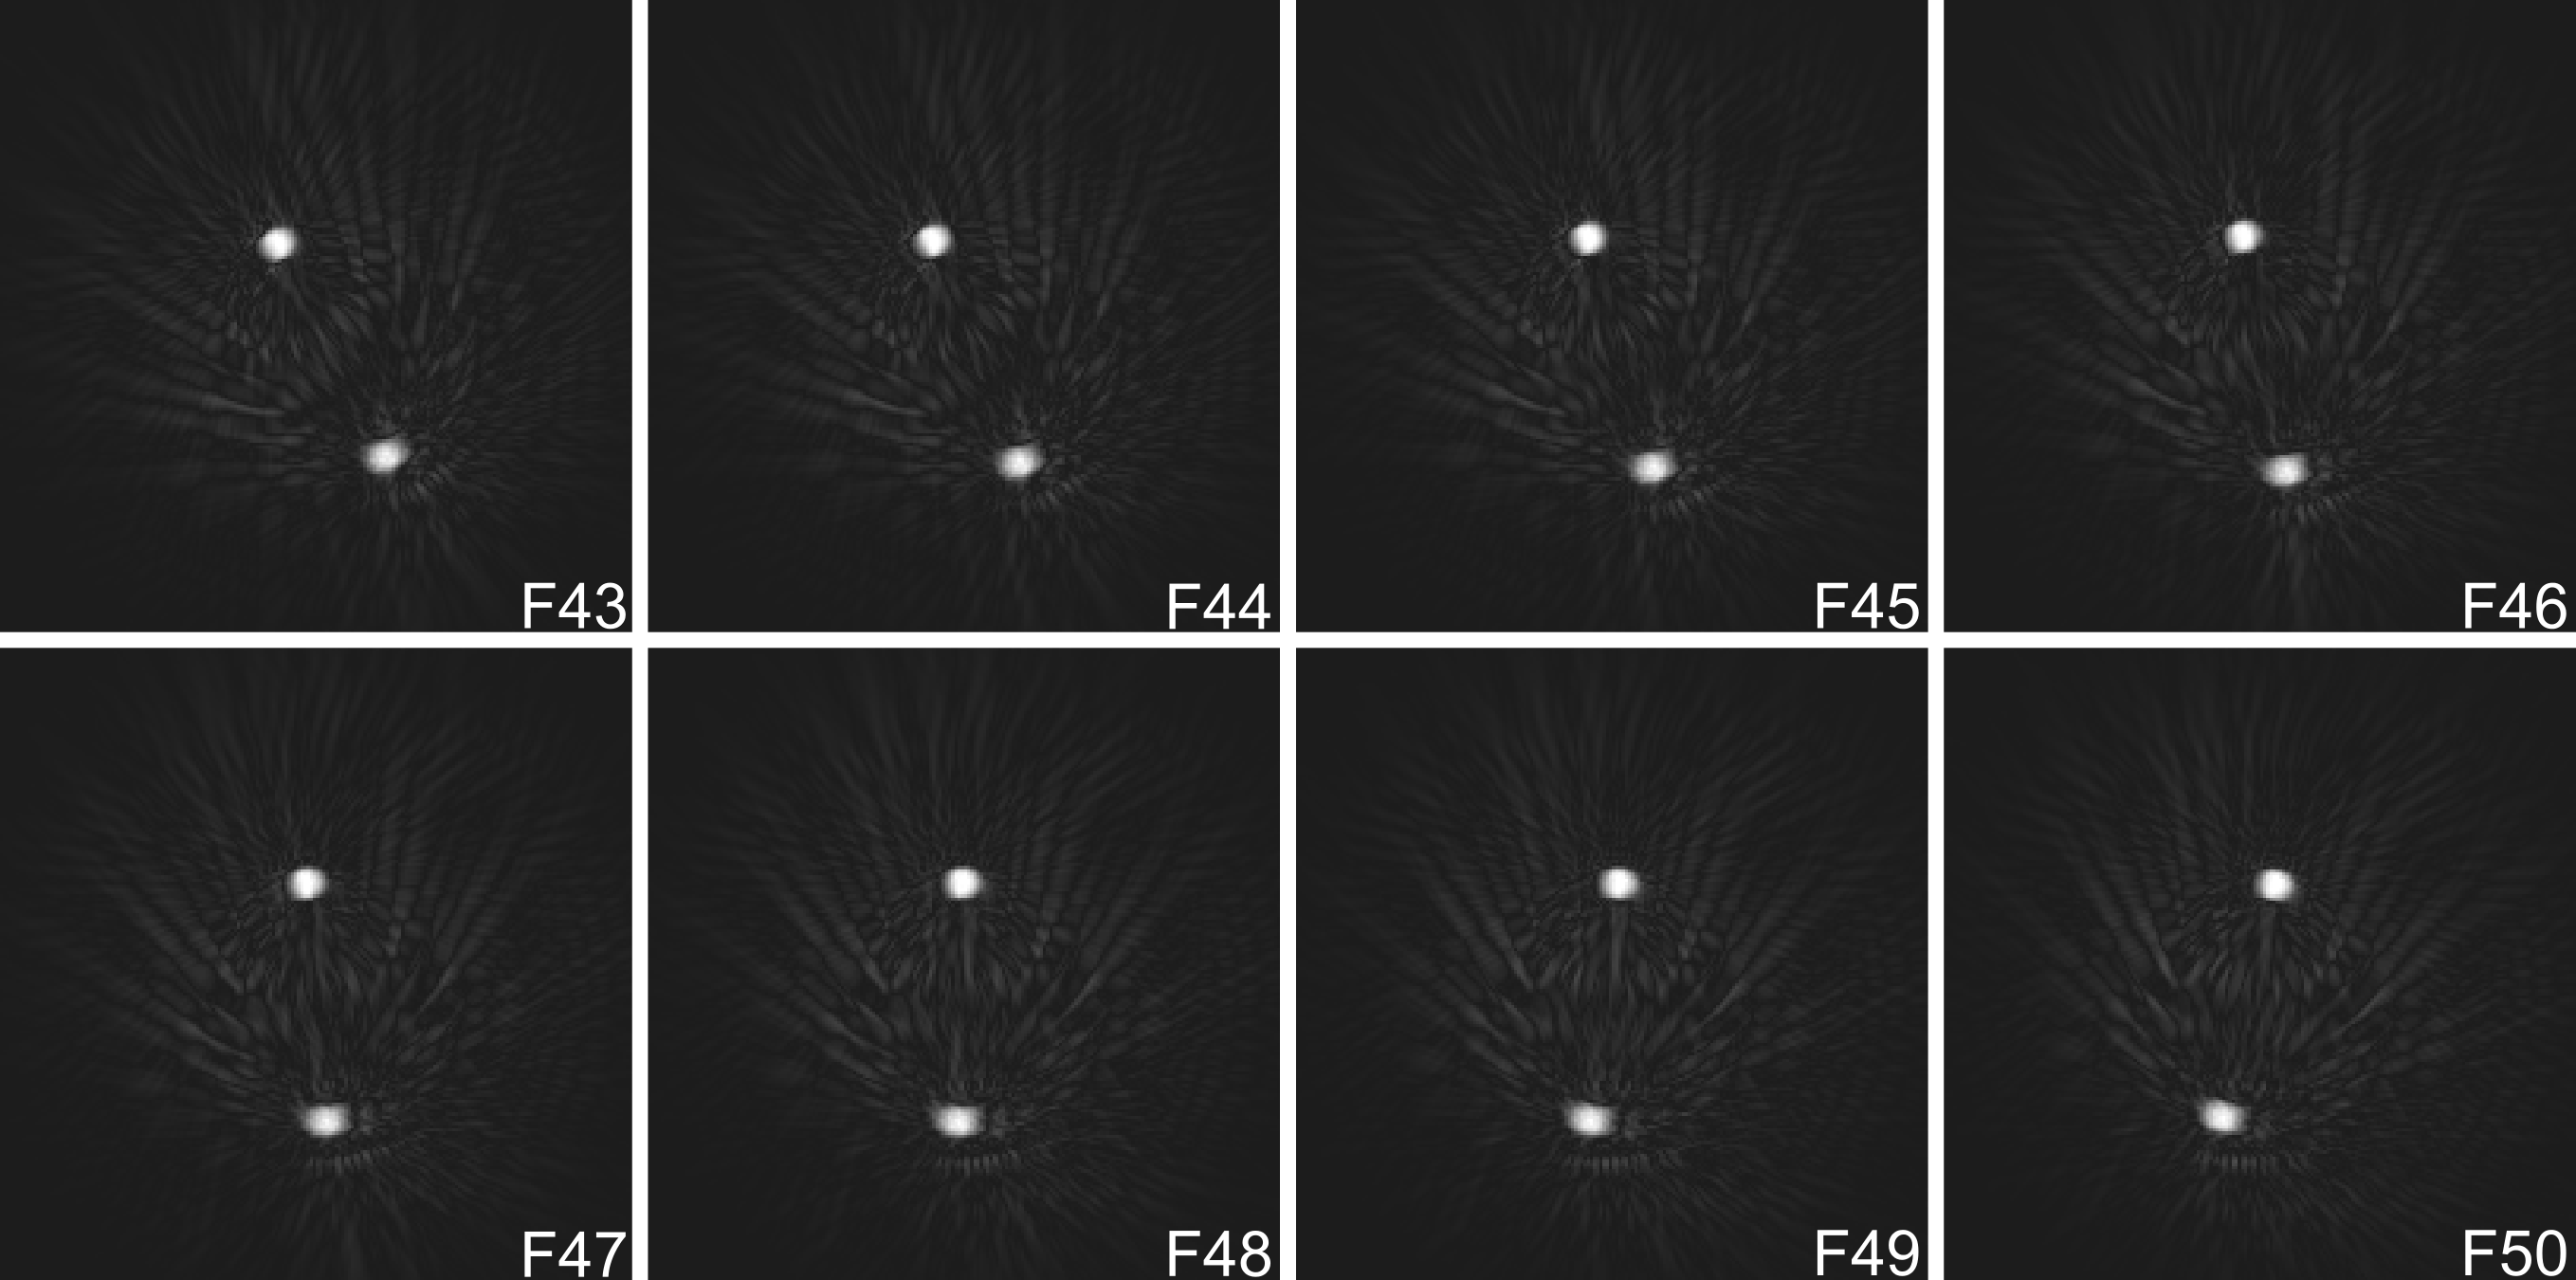
\includegraphics[width=\textwidth]{fig/sim-motion-halfPos.png}
  \caption{Eight consecutive images (from the \nth{43} to \nth{50} frame) with an in-plane rotation of $5.7^o$ per frame in the clockwise direction, base resolution 200, FOV \SI{20}{\square\cm}, \num{17} spokes per frame (\SI{33}{\ms} temporal resolution), \num{5} interleaves, \ang{360} total view angle, and \num{10} analytical coils. The images were reconstructed by NLINV without the temporal median filter.} \label{Fig:sim-motion-halfPos}
\end{figure}

\begin{figure}[tb]
  \centering
  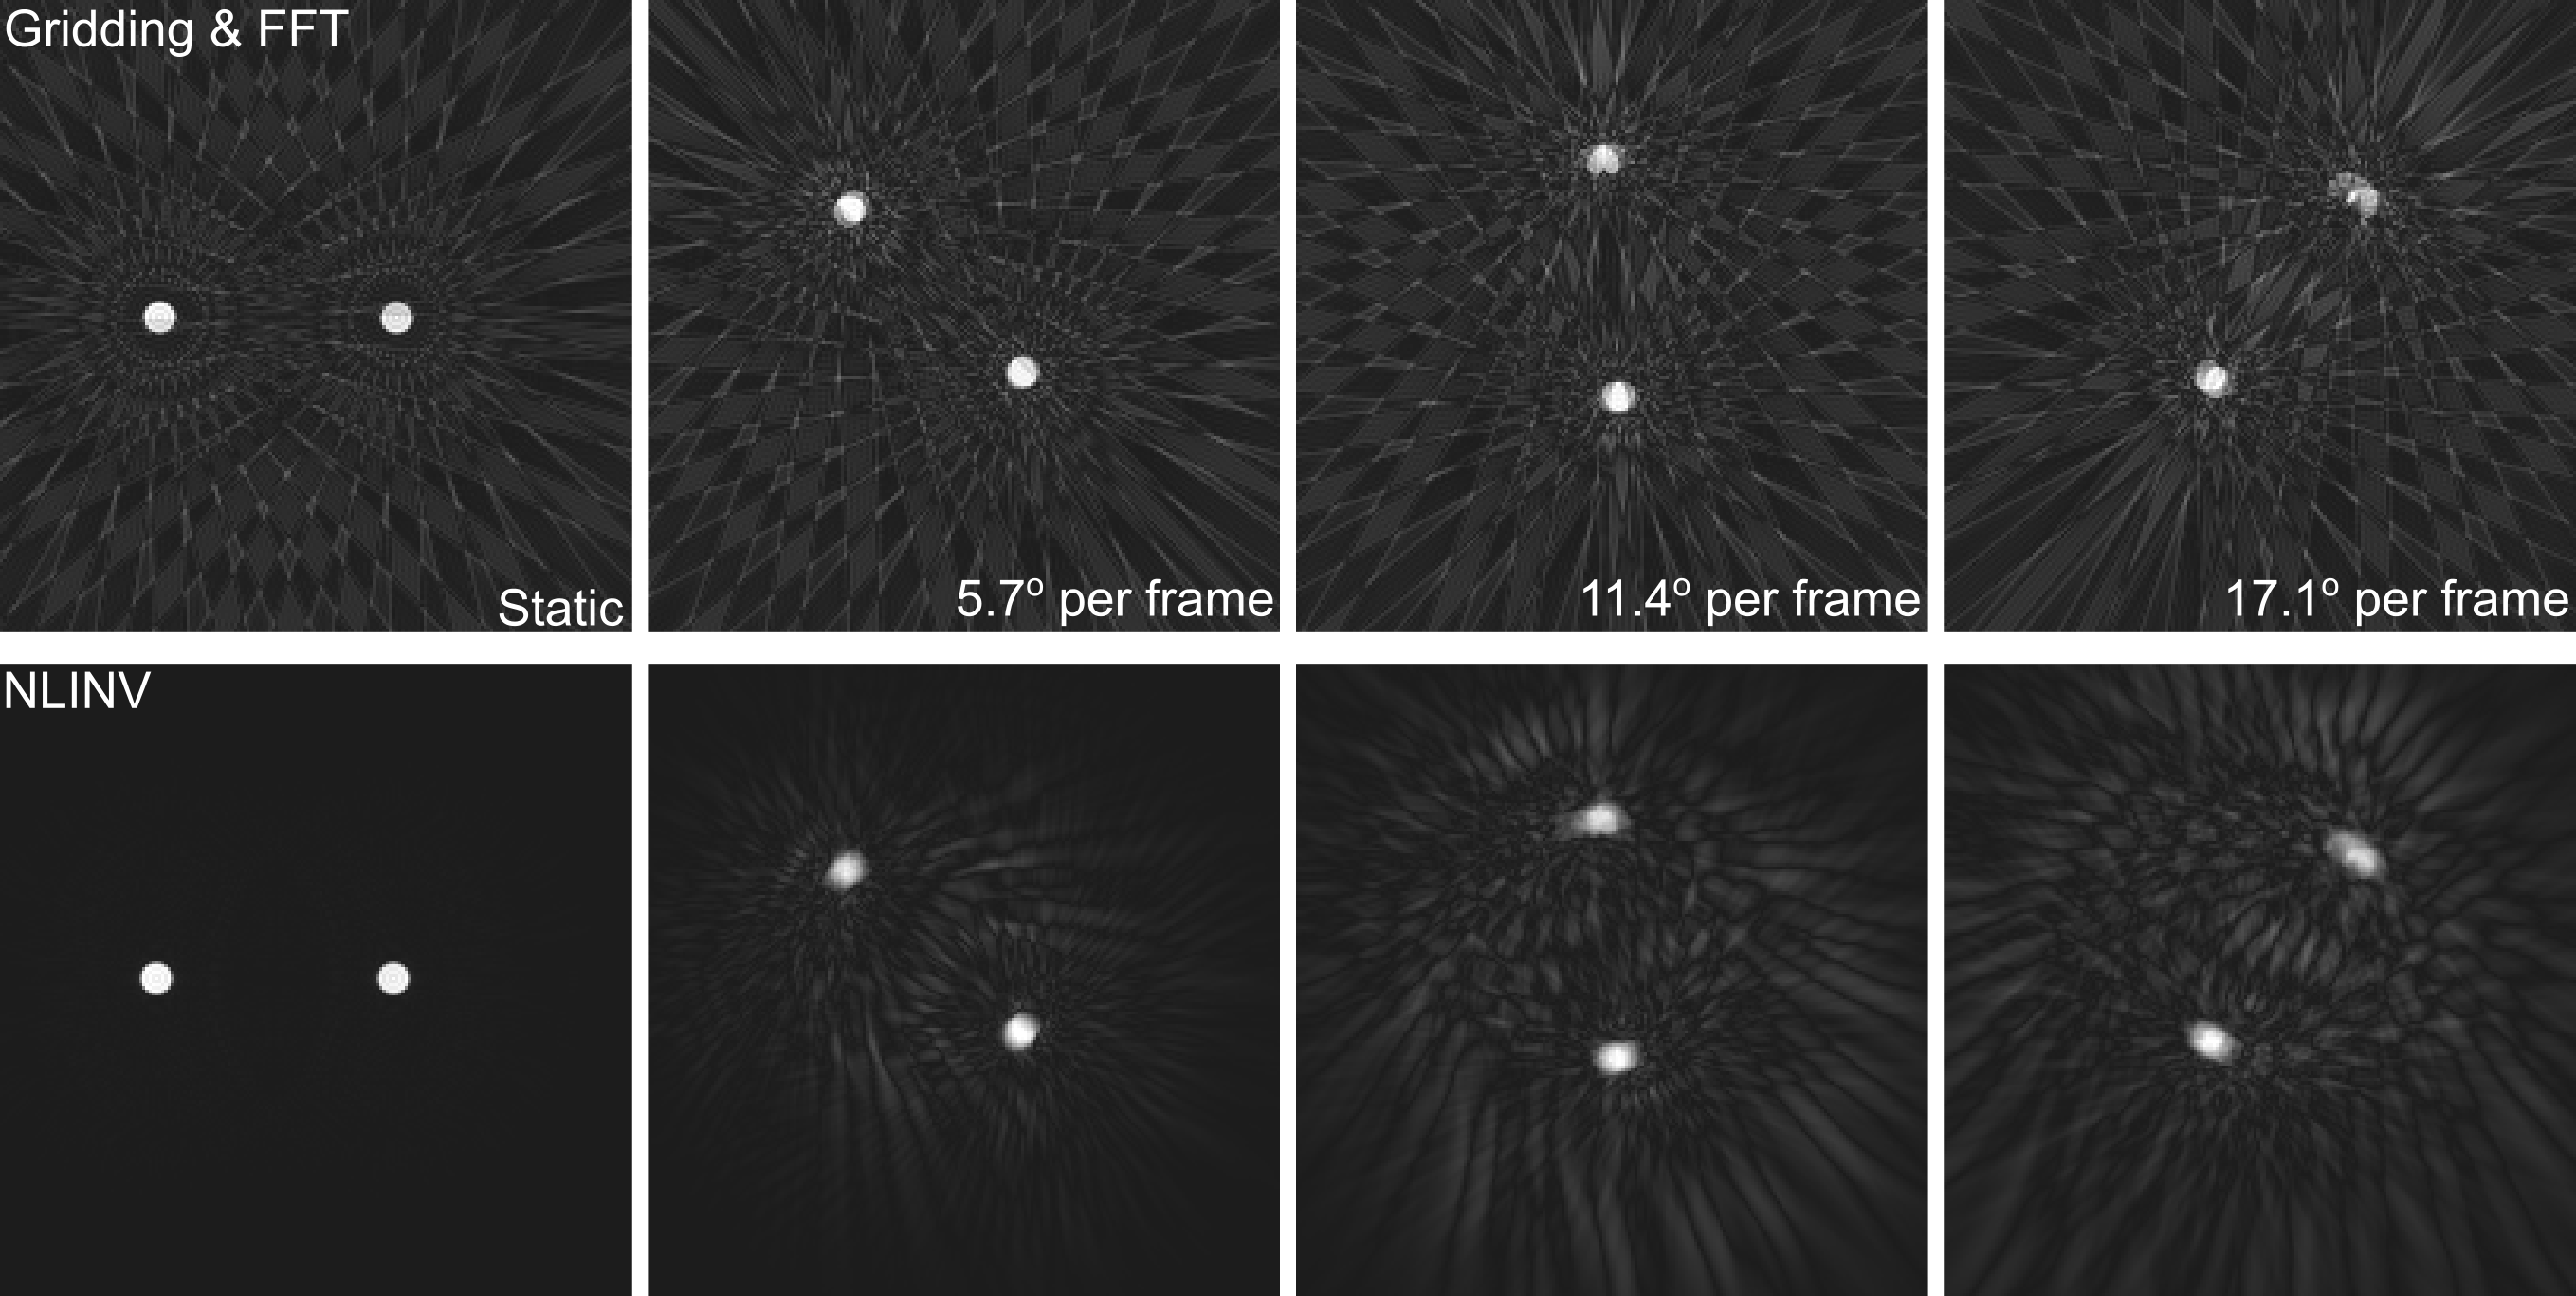
\includegraphics[width=\textwidth]{fig/sim-motion-comp.png}
  \caption{Comparisons of (top) Gridding \& FFT and (bottom) NLINV reconstructions under different rotation speeds: (1\textsuperscript{st} column) stationary, (2\textsuperscript{nd} column) \ang{5.7} per frame, (3\textsuperscript{rd} column) \ang{11.4} per frame, and (4\textsuperscript{th} column) \ang{17.1} per frame. The other acquisition parameters are identical to those in \cref{Fig:sim-motion-halfPos}.} \label{Fig:sim-motion-comp}
\end{figure}

\chapter{Asymmetric Radial Gradient Echoes}
\chaptermark{Asymmetric Radial Gradient Echoes} \label{Chp:asym-echo}

Asymmetric-echo radial sampling is an interesting sampling scheme because it shortens the echo time and thus reduces off-resonance effects. In contrast to the k-space line (echo)-reduction undersampling scheme, it samples an incomplete echo, which poses a different reconstruction problem on how to estimate the missing portion of the echo. Therefore, this chapter studies the characteristics of asymmetric radial gradient echoes and associated image reconstruction methods. Moreover, the application of this sampling scheme to real-time phase-contrast flow MRI is investigated. Here, asymmetric echoes allow for the integration of motion-compensation gradients while maintaining or even improving temporal resolution. Consequently, flow MRI with motion compensation and short \acs{TE} reduces signal loss due to intra-voxel phase dispersion and turbulence \cite{2015_PC_rev}.

\section{Undersampled Radial FLASH with Asymmetric Echoes}
For asymmetric echo data sampling, also known as partial echo in partial Fourier imaging \cite{2004_MRI_Bernstein}, every k-space readout line is only partially collected before reaching the center of k-space. This is achieved by reducing the moment of the corresponding pre-dephasing gradient, as shown in the sequence diagram (left part of \cref{Fig:aysm-echo-seq-ksp}). Therefore, it shortens the readout gradient before the echo center and reduces the TE and TR, while the readout period after the echo center remains the same as for symmetric echo. Here, an asymmetry metric (in $\%$) is quantified as $100 \times A / (2 B)$ with $A$ and $B$ the durations of the acquisition window before and after the echo center, respectively. With this definition, \SI{50}{\percent} asymmetry corresponds to a symmetric echo, while \SI{0}{\percent} represents a half-echo acquisition. The k-space trajectory depicted in the right part of \cref{Fig:aysm-echo-seq-ksp} demonstrates the extreme azimuthal undersampling with only seven spokes per image and \SI{20}{\percent} asymmetry.

As has been demonstrated in \cite{2004_MRI_Bernstein}, the first row of \cref{Fig:aysm-echo-psf} shows that the artifact-free area of the simulated point spread functions (\acsp{PSF}) reconstructed via direct Gridding \& FFT decreases along the number of symmetric spokes acquired, but the central lobe is not distorted or folded-in as is commonly seen in undersampled Cartesian sampling. Furthermore, the streaks are much better spatially resolved and more severe with less number of spokes. On the other hand, when the number of spokes is kept at \num{125} and the asymmetry is reduced from \SI{40}{\percent} to \SI{30}{\percent} and \SI{20}{\percent} (see the second row of \cref{Fig:aysm-echo-psf}), a bright ring surrounding the central white lobe emerges and eventually reduces the artifact-free area. This may result in blurring and Gibbs ringing artifacts due to the lack of high spatial-frequency data. 
\begin{figure}[p]
  \centering
  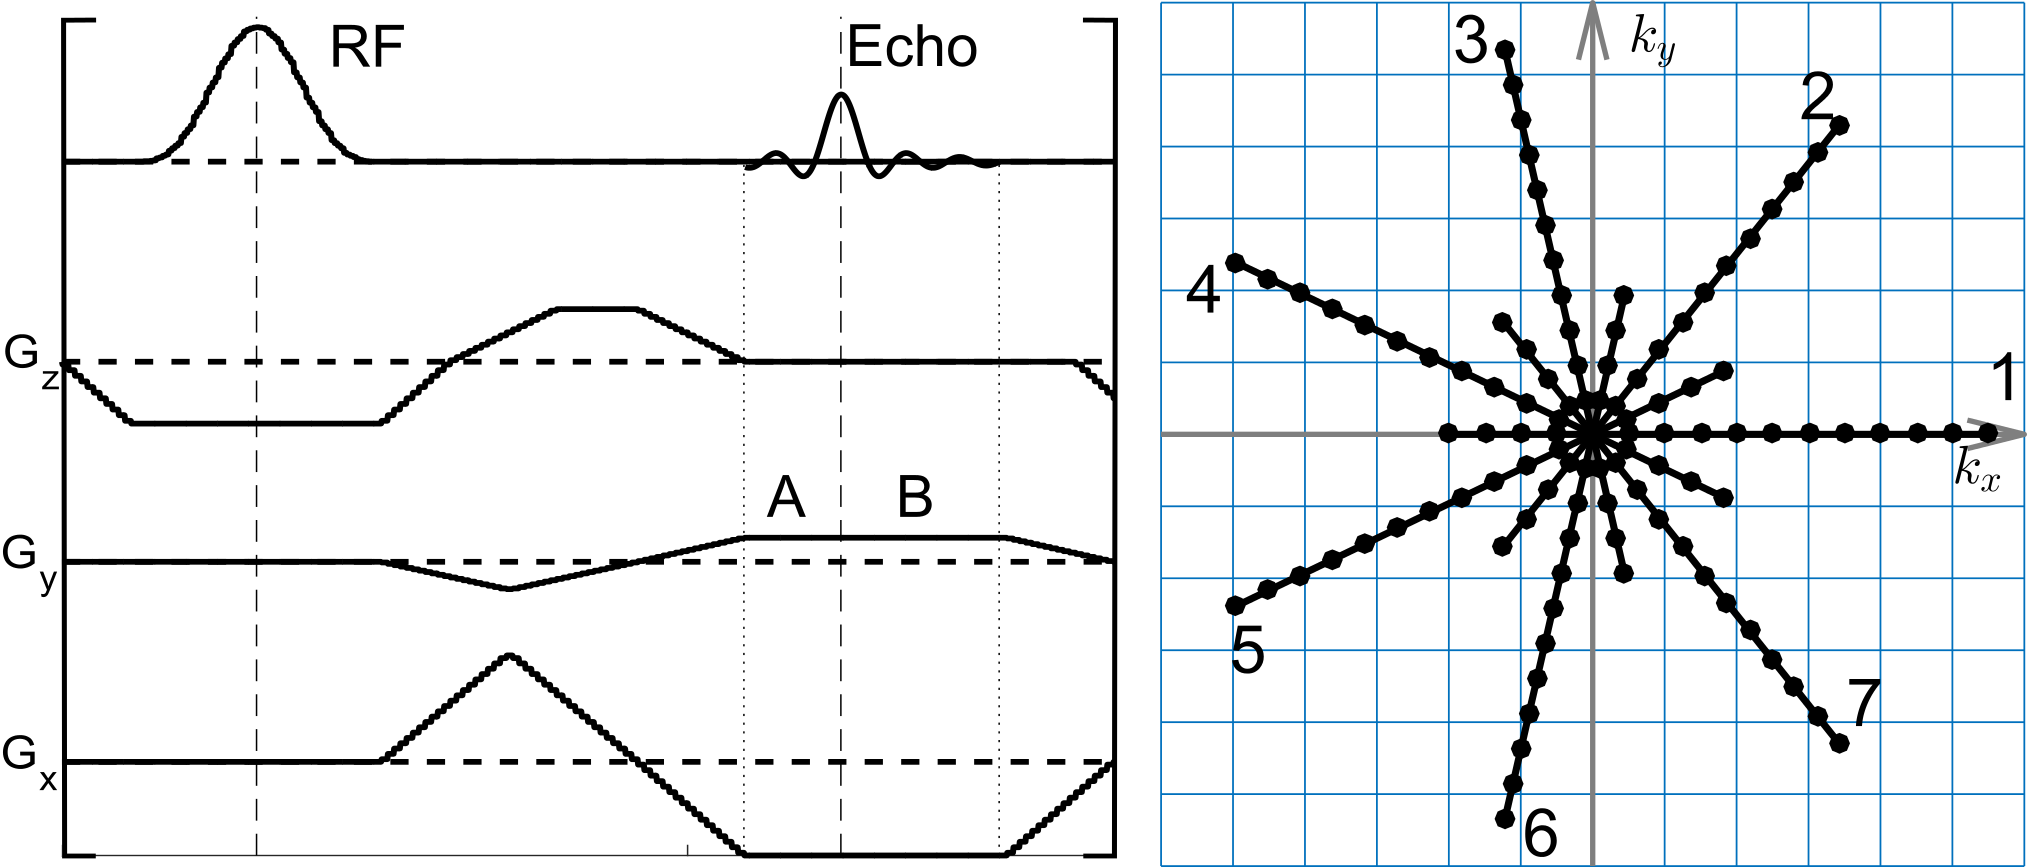
\includegraphics[width=0.85\textwidth]{fig/asym-echo-seq-ksp.png}
  \caption{Real-time radial FLASH with asymmetric gradient echoes. Left: The sequence diagram represents one repetition cycle for the acquisition of one asymmetric echo. Right: Corresponding k-space trajectory with seven spokes with \SI{20}{\percent} asymmetry and $2\pi$ radial angle coverage. The blue lines represent a 2D Cartesian grid. } \label{Fig:aysm-echo-seq-ksp}
  
  \par\bigskip
  
  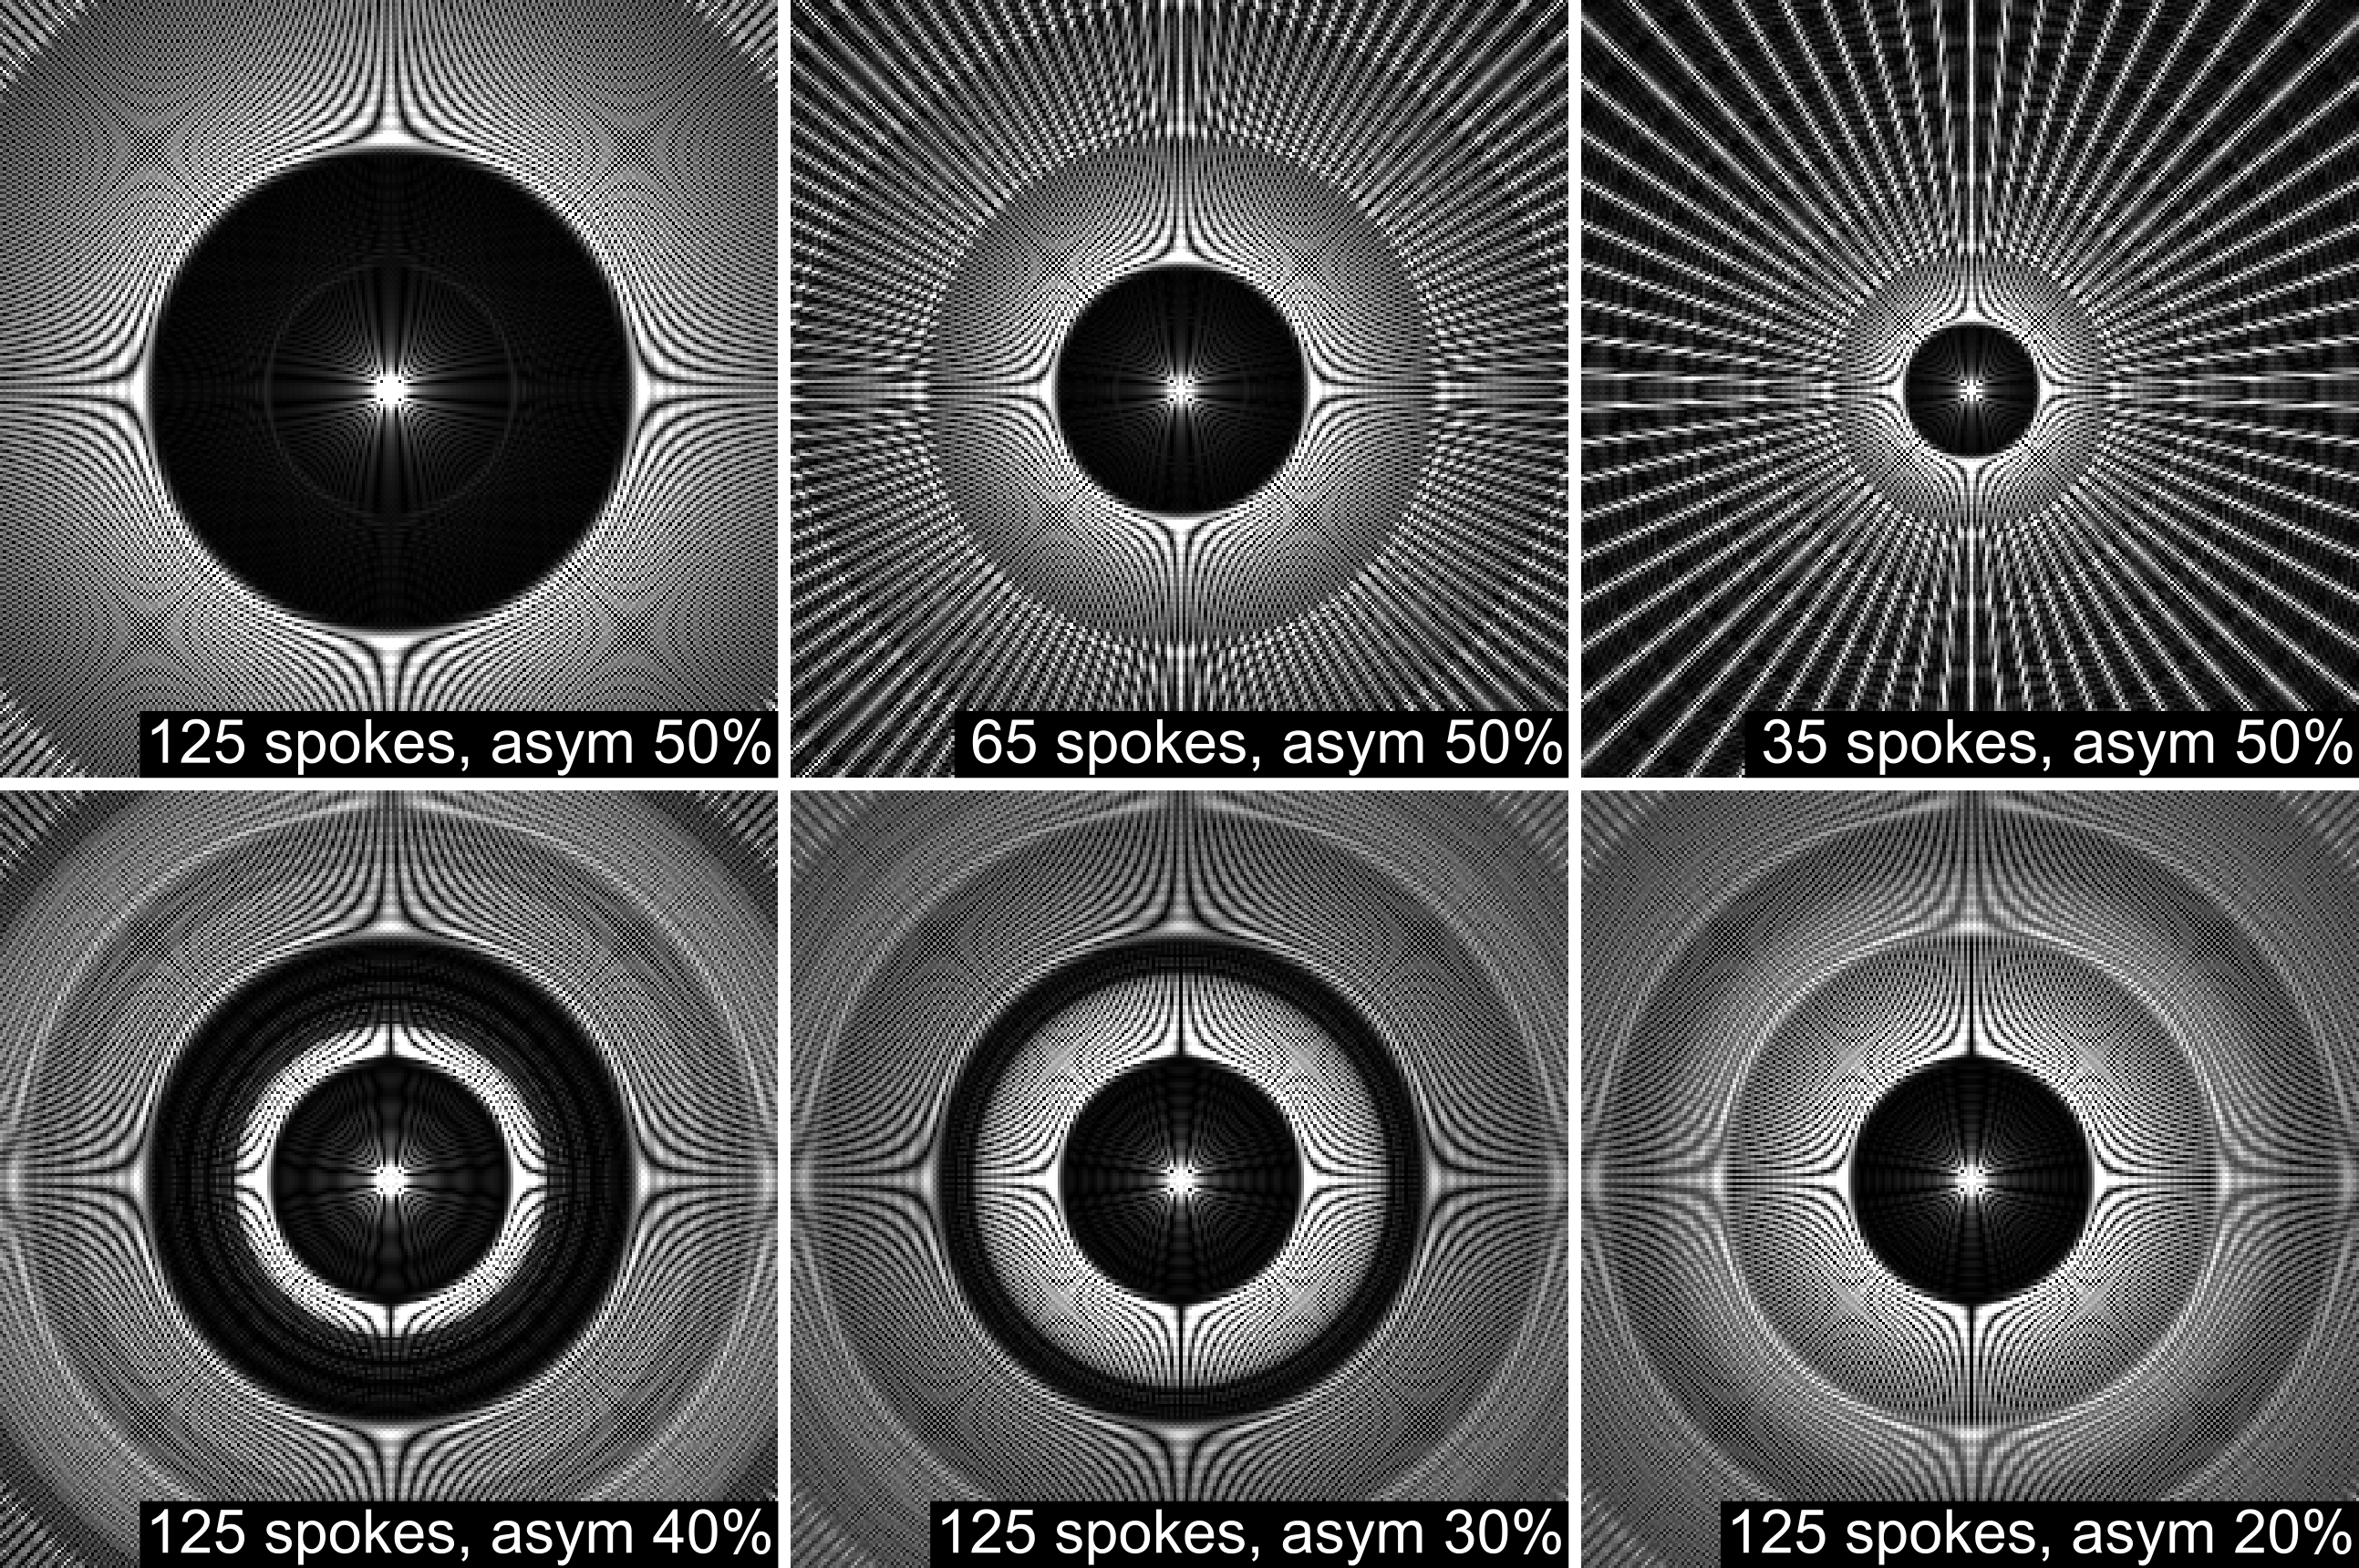
\includegraphics[width=0.85\textwidth]{fig/asym-echo-psf.png}
  \caption{Simulated \acsp{PSF} via Gridding \& FFT reconstruction with $2\pi$ radial angle coverage, 256 total readout samples. The \acs{PSF} in the first row was acquired with (left) \num{125}, (center) \num{65}, and (right) \num{35} symmetric spokes, while the second row was acquired with 125 spokes and (left) \SI{40}{\percent}, (center) \SI{30}{\percent}, and (right) \SI{20}{\percent} asymmetry. The central white lobe of the \acsp{PSF} indicates the reconstructed point. The artifact-free area is the solid black region around the central lobe.} \label{Fig:aysm-echo-psf}
\end{figure}

Another appealing feature of asymmetric echo is that it keeps the same spatial resolution as symmetric echo. It is well known that the spatial resolution is inversely proportional to the maximum gradient areas in two readout directions, which are equivalent to $k_{x,\text{max}}$ and $k_{y,\text{max}}$, respectively \cite{2010_principle_mri}. As the radially-supported FOV in k-space for asymmetric echo is the same as that for symmetric echo, the spatial resolution retains for asymmetric-echo sampling. As shown in \cref{Fig:aysm-echo-spatialRes}, where simulated asymmetric k-space data was generated from a symmetric measurement (i.e.~\SI{50}{\percent} asymmetry) for a standard multi-purpose phantom of the vendor. Respective FLASH acquisition parameters were: TR/TE = \num{2.48}/\SI{1.62}{\ms}, flip angle \ang{8}, \SI{212}{\mm} FOV, \SI{0.83}{\mm} in-plane resolution, \SI{8}{\mm} slice thickness, \num{15} spokes and \num{5} sequential-interleaving turns. Simulated gradient-echo data with \SI{40}{\percent}, \SI{30}{\percent}, and \SI{20}{\percent} asymmetry were obtained by cropping a respective number of data samples from the leading parts of corresponding symmetric spokes. True asymmetric measurements of the resolution phantom for \SI{40}{\percent}, \SI{30}{\percent}, and \SI{20}{\percent} asymmetry used similar experimental parameters as the symmetric measurement except for the shortest possible repetition and echo times: TR/TE (\SI{40}{\percent}) = \num{2.31}/\SI{1.45}{\ms}, TR/TE (\SI{30}{\percent}) = \num{2.14}/\SI{1.28}{\ms}, and TR/TE (\SI{20}{\percent}) = \num{1.99}/\SI{1.13}{\ms}. The spatial resolution of all images in \cref{Fig:aysm-echo-spatialRes} is well maintained, although increasing asymmetry leads to fewer samples in the outer (e.g.~high spatial frequency) regions of k-space. This is clearly demonstrated by the well-resolved first three rows of water-filled holes in \cref{Fig:aysm-echo-spatialRes} with diameters ranging from \SI{2.5}{\mm} to \SI{2.0}{\mm} and \SI{1.5}{\mm}.
\begin{figure}[tb]
  \centering
  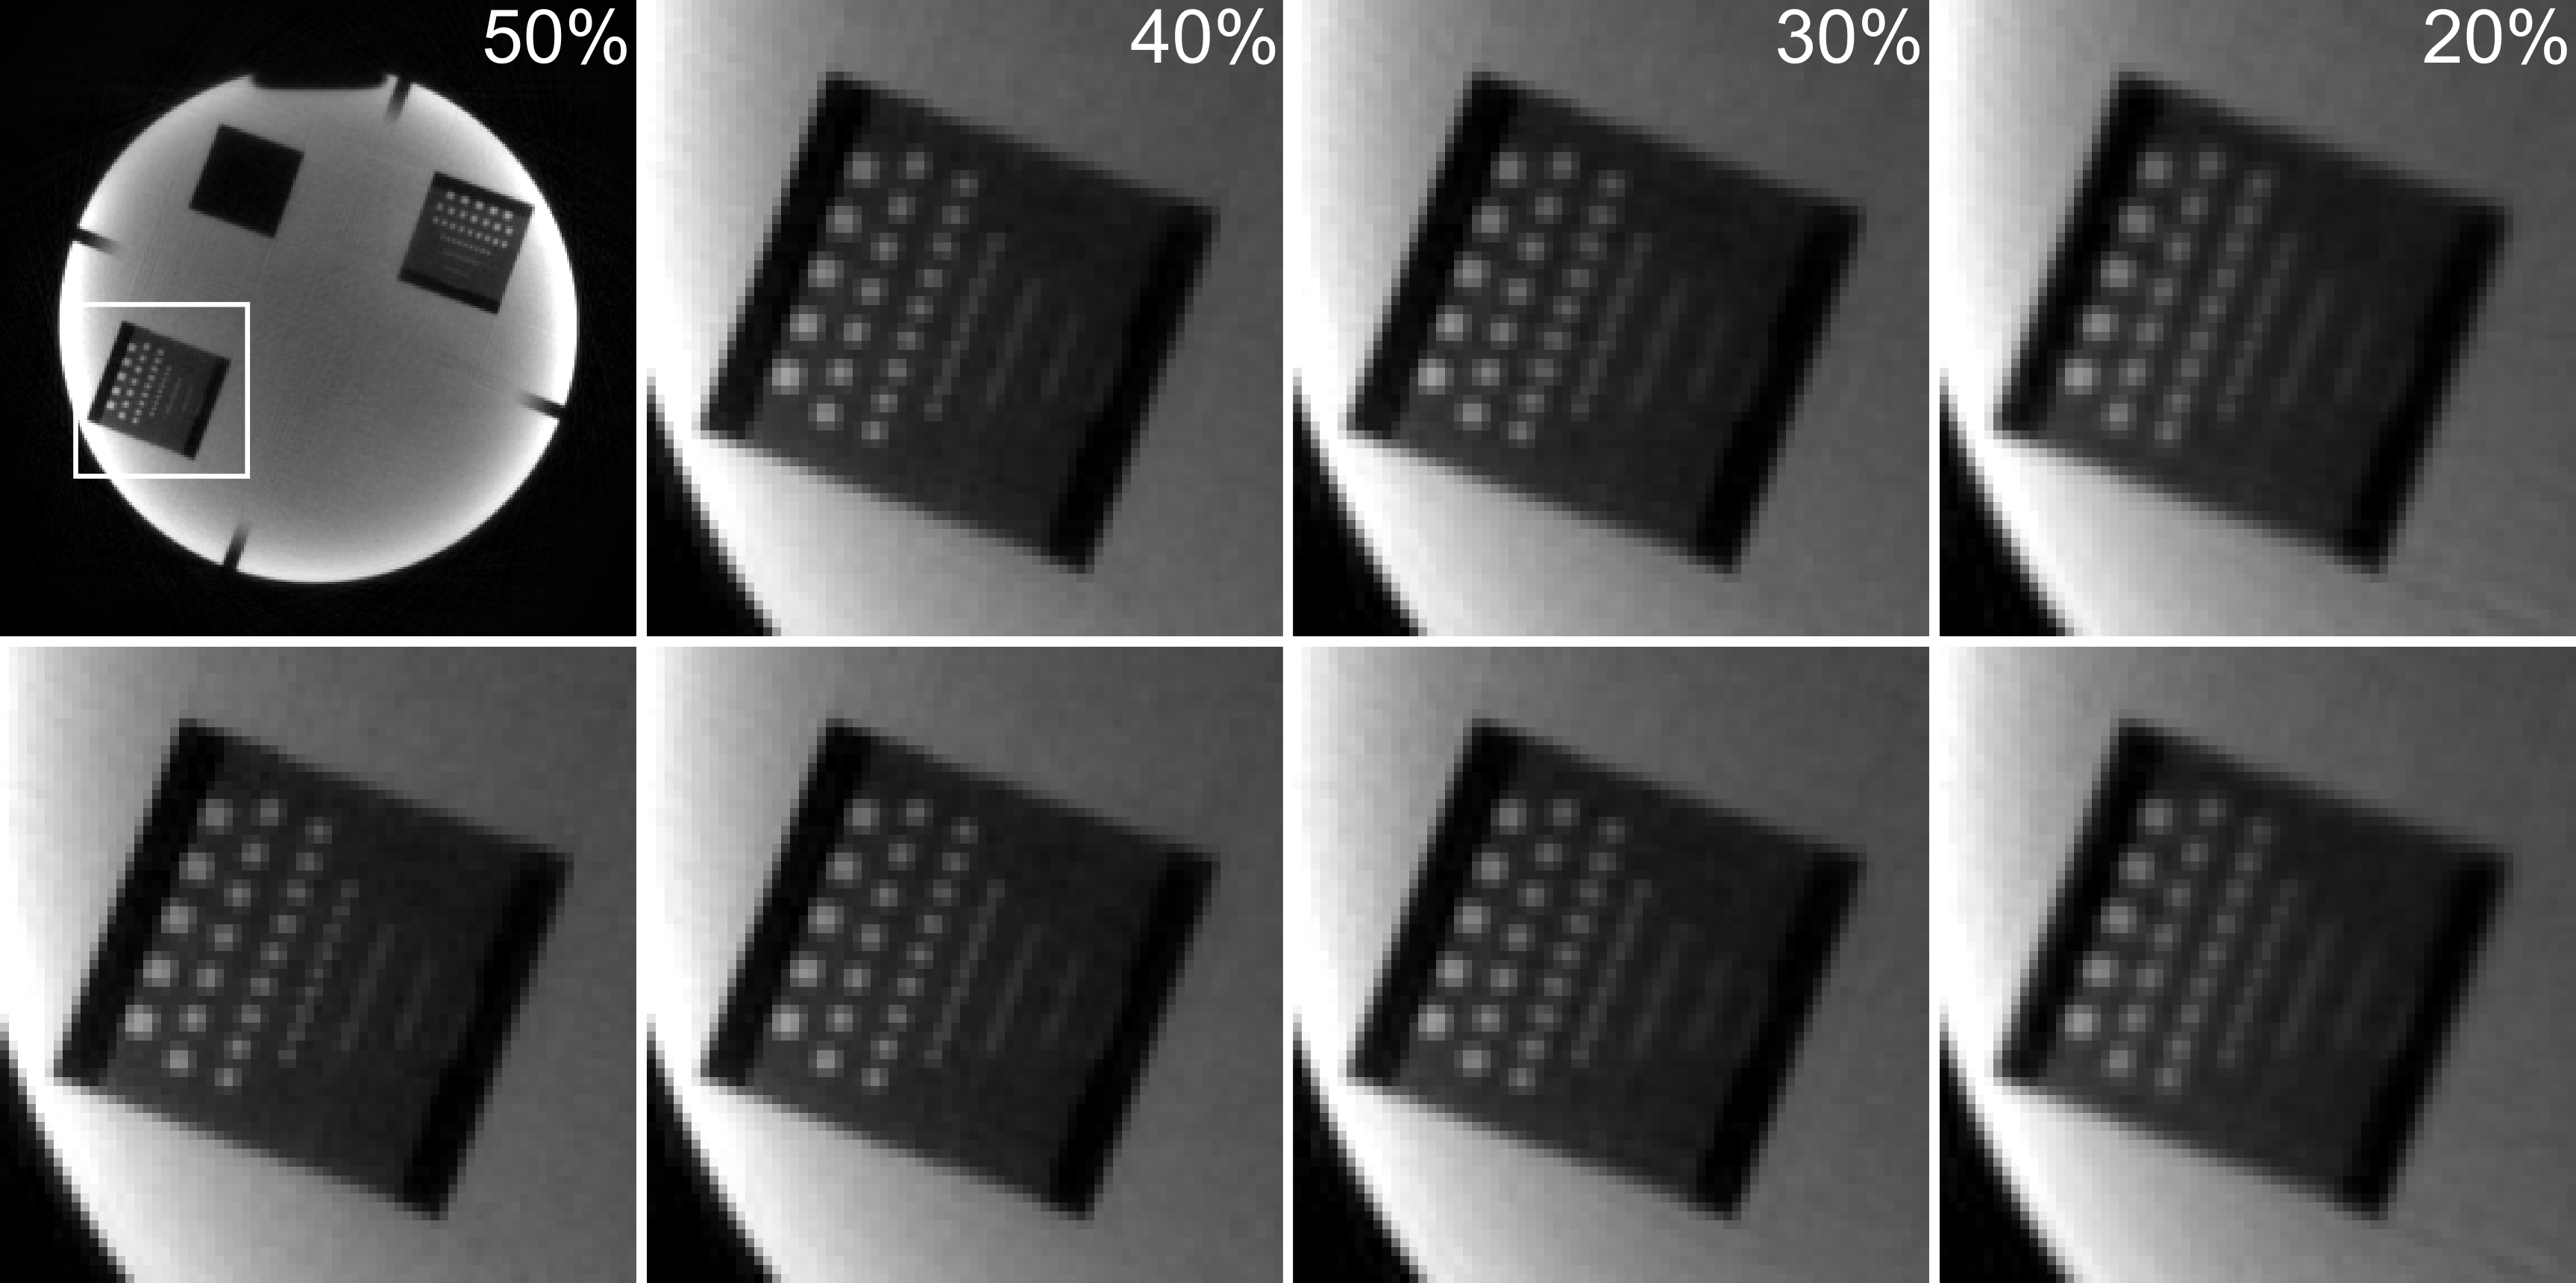
\includegraphics[width=\textwidth]{fig/asym-echo-spatialRes.png}
  \caption{Image reconstructions of a resolution phantom using symmetric gradient echoes (\SI{50}{\percent}) as well as gradient echoes with \SI{40}{\percent}, \SI{30}{\percent}, and \SI{20}{\percent} asymmetry. For asymmetric cases the top panels refer to simulated data obtained by retrospective cropping of data samples of complete spokes, while the bottom panels represent true asymmetric acquisitions with shortest TR and TE. The size of the water-filled holes (and gaps between) in the first three rows are \SI{2.5}{\mm}, \SI{2.0}{\mm}, and \SI{1.5}{\mm} respectively.} \label{Fig:aysm-echo-spatialRes}
\end{figure}

Furthermore, the reduction of TE in asymmetric-echo sampling reduces the sensitivity to off-resonance effect. This property is advantageous in imaging tissues with small $T_2^*$ (e.g.~lung imaging) and slices with strong susceptibilities (e.g.~air-tissue interface). 

\section{Image Reconstructions}
Partial Fourier imaging exploits the conjugate complex symmetry of the full k-space of a real image with zero phase. It is, therefore, widely used to accelerate the acquisition of radiofrequency-refocused spin-echo images. For most gradient-echo images, however, the real-image assumption is violated due to system imperfections and off-resonance contributions from various biological and technical sources, which render the image complex. Previous proposals to deal with complex datasets are synchronous homodyne detection \cite{1991_homodyne}, the projection onto convex sets (\acs{POCS}) method \cite{1991_POCS}, and phase-constrained parallel imaging \cite{2005_PFPPI,2005_phaConstrain_PI}. These approaches assume a certain smoothness of the image phase to justify the calculation of a low-resolution phase map from only the central (i.e. symmetrically covered) k-space region, which is then used to estimate the missing data. More advanced image reconstruction technique, e.g.~NLINV, can directly apply a real-constraint onto the estimated proton density without the pre-calibration of a smooth phase map from the central k-space \cite{2009_Uecker_Thesis}. This real-constrained NLINV, however, totally relies on the conjugate complex symmetry and hence precludes the imaginary part of the estimate proton density, which is insufficient in the cases where phase information is required, e.g., phase-contrast flow imaging and quantitative susceptibility mapping. This study, therefore, exploited the general applicability of NLINV to directly reconstruct complex images and coil sensitivity maps from undersampled asymmetric radial gradient-echo acquisitions.

\section{Application to Real-Time Phase-Contrast Flow MRI}
The implementation of real-time phase-contrast flow MRI is especially challenging because it requires at least two acquisitions with different velocity-encoding gradients that prolong echo times and repetition times. Additional timing problems arise for the incorporation of velocity-compensating gradient waveforms in multiple dimensions. Therefore, this work extends earlier attempts to real-time phase-contrast flow MRI using spiral trajectories \cite{2000_color_flow_MRM,2008_color_flow_MRI} as well as our own recent approaches \cite{2012_PC_Joseph,2014_PC_Joseph} by evaluating the use of asymmetric echoes for radial FLASH sequences with phase-sensitive NLINV reconstruction. The technique advances proposals of asymmetric radial trajectories for ECG-synchronized cine MRI \cite{2014_asym-echo_ISMRM,2014_sTE_flow_ISMRM} to highly undersampled acquisitions suitable for real-time MRI as high temporal resolution. In general, shorter gradient-echo times may be used to reduce the sensitivity to magnetic field inhomogeneities, to acquire more data, to enhance the temporal resolution or to ameliorate the time penalty of motion-compensating gradient waveforms. In short, the purpose of this work was to explore asymmetric radial gradient echoes for real-time phase-contrast flow MRI to allow for velocity compensation in both slice and read directions and thereby reduce the sensitivity of complex blood flow and respective phase errors as commonly observed in patients with cardiovascular disease.

\subsection{Methods}
\cref{Fig:aysm-echo-seq-pc} shows a phase-contrast flow MRI sequence with asymmetric-echo radial FLASH. The sequence diagrams represent two repetitions without and with velocity-encoding gradient, corresponding to the one-sided velocity-encoding scheme. The two TR intervals represent the same spoke from sequential image acquisition (flow-compensated acquisition first and then flow-encoded acquisition, and these two acquisitions encode the same spokes in k-space). The diagrams correctly display the used gradient waveforms (i.e., durations and strengths) for \SI{30}{\percent} asymmetry and VENC = \SI{150}{\cm\per\second} (for other parameters see \cref{Tab:asym-echo-acq}).
\begin{figure}[tb]
  \centering
  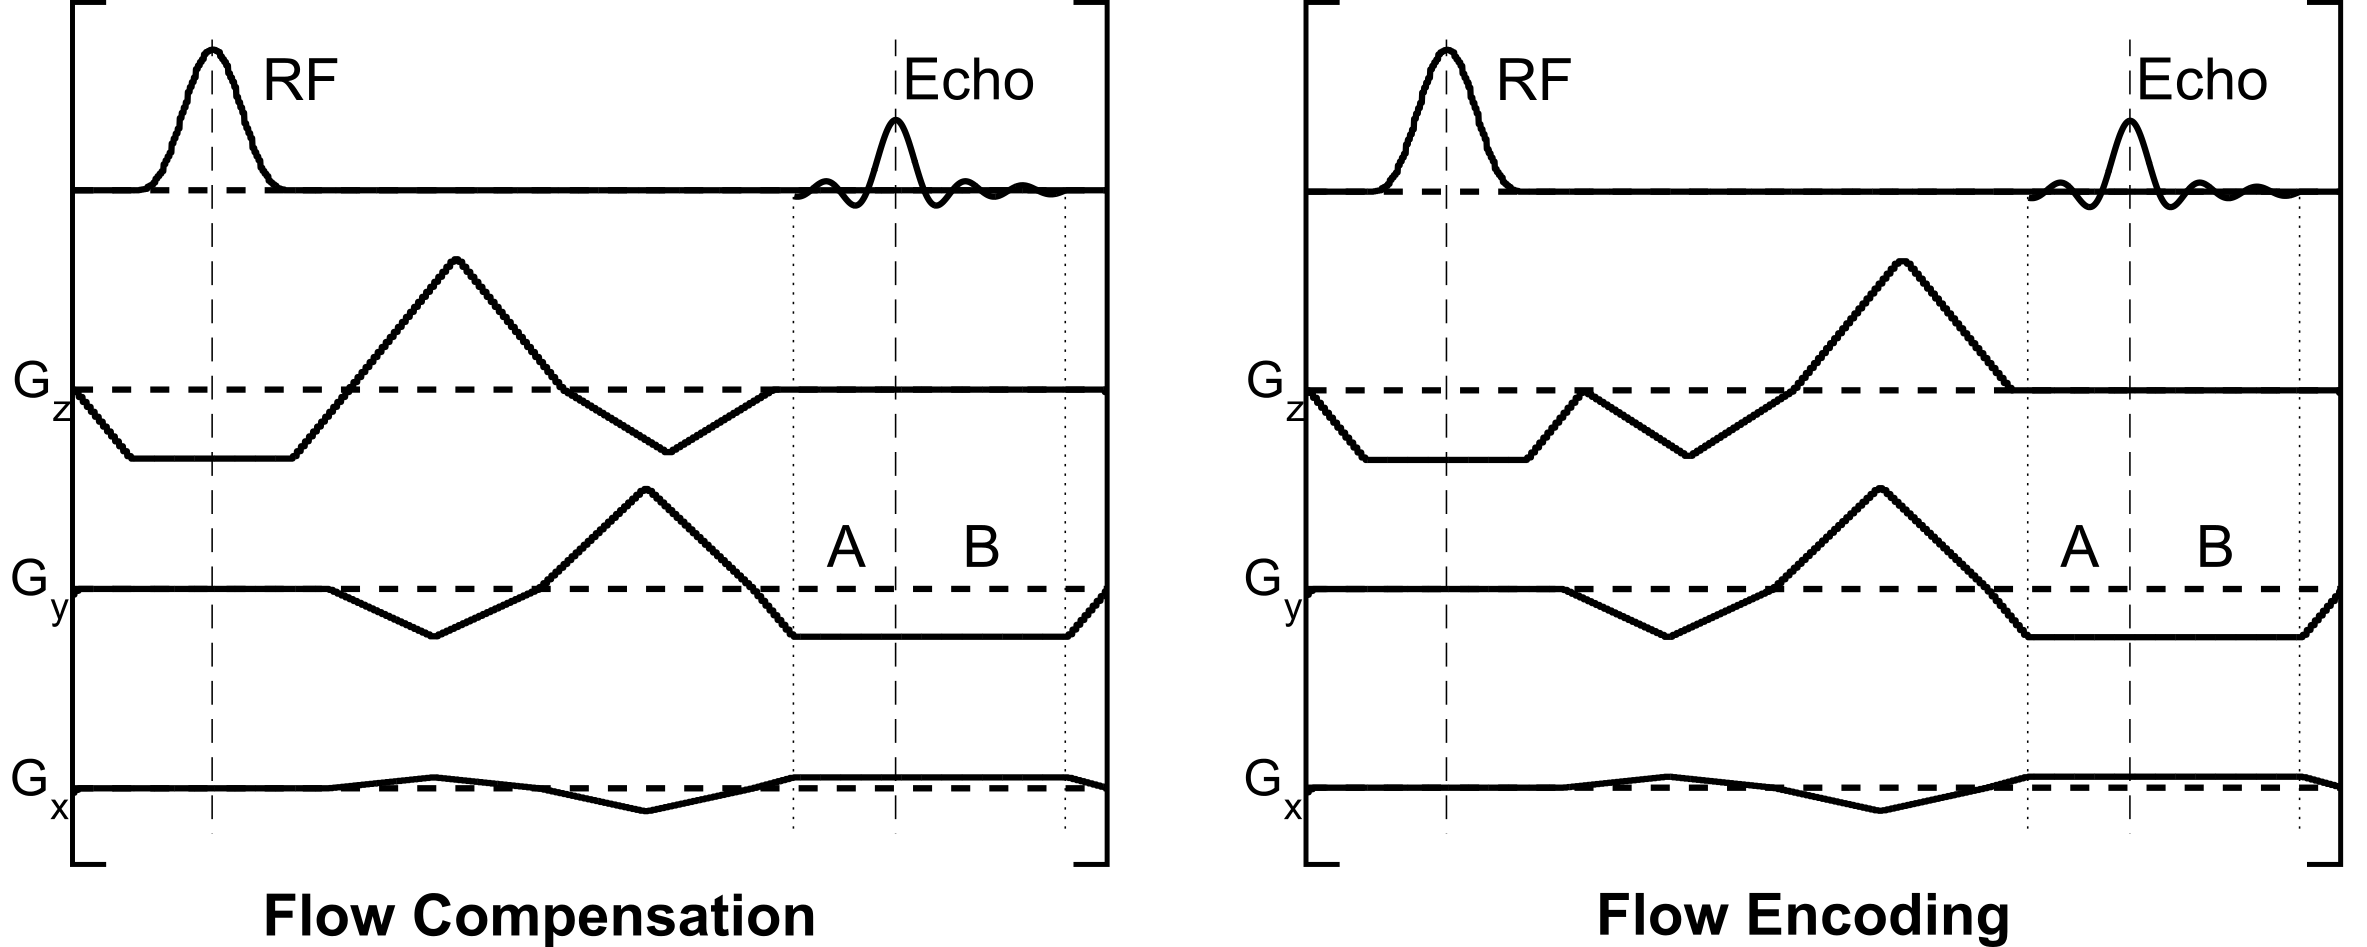
\includegraphics[width=\textwidth]{fig/asym-echo-seq-pc.png}
  \caption{Real-time velocity-encoded radial FLASH with velocity compensation and asymmetric gradient echoes. The sequence diagrams represent corresponding repetition cycles: (Left) Acquisition with velocity-compensated gradients with the waveform $1 \bar{2} 1$ on all axes and overlap the slice selection gradient and the two prephasing read gradients, respectively. (Right) Acquisition with velocity-encoded gradient on the slice selection axis to encode through-plane velocities, and with velocity-compensated gradients on the two read axes to spoil transversal motions.} \label{Fig:aysm-echo-seq-pc}
\end{figure}

\begin{table}[tb]
  \caption{Exemplary acquisition parameters for real-time phase-contrast flow MRI}
  \label{Tab:asym-echo-acq}
  \begin{center}
	\begin{tabular}{ l 
					 c 
					 c 
				   }
	  \toprule
	  Field of view (\si{\square\mm})        & $192 \times 192$        & $320 \times 320$ \\
	  Image matrix size                      & $136 \times 136$        & $212 \times 212$ \\
	  In-plane resolution (\si{\square\mm})  & $1.4 \times 1.4$        & $1.5 \times 1.5$ \\
	  Section thickness (\si{\mm})           & $6$                     & $6$              \\
	  Asymmetry                              & \SI{20}{\percent}     & \SI{30}{\percent} \\
	  Minimum VENC (\si{\cm\per\second})     & $150$                   & $150$               \\
	  Velocity compensation                  & Slice \& $2\times$ Read & Slice \& $2\times$ Read \\
	  Repetition time (\si{\ms})             & 2.38                  & 2.55 \\
	  Echo time (\si{\ms})                   & 1.59                  & 1.70 \\
	  Bandwidth (\si{\hertz\per\pixel})      & 1360                  & 1180 \\
	  Flip angle (\si{\degree})              & 10                    & 10 \\
	  Spokes per frame                       & 7                     & 7 \\
	  Time per frame (\si{\ms})              & 16.66                 & 17.85 \\
	  Time per phase-contrast map (\si{\ms}) & 33.32                 & 35.70 \\
	  Temporal resolution (\si{\fps})        & 30                    & 28 \\
	  \bottomrule
    \end{tabular}
  \end{center}
\end{table}

Five young volunteers without known illness and one patient with combined aortic valve insufficiency and stenosis were recruited for real-time phase-contrast flow evaluations of the ascending aorta. Written informed consent, according to the recommendations of the local ethics committee, was obtained from all subjects before MRI studies, which were performed at \SI{3}{\tesla} using a state-of-the-art MRI system with \SI{80}{\milli\tesla\per\meter} gradients (Magnetom Prisma, Siemens Healthcare, Erlangen, Germany). While phantom studies used the standard \num{64}-channel head coil, human cardiac blood flow was measured by combining an \num{18}-element thorax coil with \num{32} elements of the spine coil. 

For real-time phase-contrast flow MRI with velocity compensation in slice and read directions the outcome of the sequence optimization and reconstruction process led to multiple acquisition protocols. Two relevant examples for a small and large FOV are summarized in \cref{Tab:asym-echo-acq}. In comparison to echo and repetition times of TR/TE = \num{2.86}/\SI{1.93}{\ms} previously reported for symmetric-echo acquisitions without in-plane velocity compensation and a measuring time of \SI{40}{\ms} \cite{2014_PC_Joseph}, the current values of TR/TE = \num{2.38}/\SI{1.59}{\ms} (FOV = \SI{192}{\mm}) and TR/TE = \num{2.55}/\SI{1.70}{\ms} (FOV = \SI{320}{\mm}) offer even faster acquisitions with total measuring times of \SI{33.3}{\ms} and \SI{35.7}{\ms}, respectively. While these numbers refer to a minimum VENC of \SI{150}{\cm\per\second}, the latter implementation would be prolonged to \SI{40}{\ms} when using \SI{75}{\cm\per\second}.

Blood flow was measured in the ascending aorta at the level of the right pulmonary artery. Typically, real-time flow MRI acquisitions of human subjects were performed during free breathing at \SI{35.7}{\ms} resolution and for a period of \SI{12.5}{\second} yielding \num{350} magnitude images and phase-contrast maps. For comparison, free-breathing ECG-synchronized cine phase-contrast flow MRI with Cartesian encoding and retrospective sorting (standard sequence of the vendor) was performed at \SI{1.54 x 1.54}{\mm} in-plane resolution and \SI{6}{\mm} section thickness. This conventional technique also used velocity compensation for all imaging gradients. Other experimental parameters: TR = \SI{20.00}{\ms}, TE = \SI{2.73}{\ms}, flip angle = \ang{20}, \num{3} averages, \num{30} cardiac phases, FOV = \SI{220 x 320}{\square\mm}, matrix resolution \num{144x208}.

Before NLINV reconstruction, the datasets from multiple coils are first corrected for gradient delay errors \cite{2015_PC_Asym} and then compressed to \num{10} virtual channels with coefficients calculated by principal component analysis to reduce the amount of computational load for image reconstruction. After NLINV, quantitative analyses of phase-contrast flow MRI images and evaluations of respective flow parameters were obtained with the use of CAIPI prototype software (Franhofer MEVIS, Bremen, Germany), especially modified for the automated analysis of real-time MRI acquisitions (typically \num{10} cardiac cycles).


\subsection{Results}
\subsubsection*{Phantom Studies}
\cref{Fig:aysm-echo-pha} summarizes the results of a real-time phase-contrast flow MRI study of a phantom where the left and right panels refer to perpendicular image orientations. All magnitude images and corresponding phase-contrast maps represent selected single frames from real-time phase-contrast flow MRI movies at \SI{33.3}{\ms} resolution with velocity compensation (top) in slice direction and (bottom) in slice and read directions (experimental details in \cref{Tab:asym-echo-acq}). The rapid water flow in the inner tubing (in reverse direction to slower flow in the outer tubing) is characterized by turbulence. With velocity compensation in slice direction only and symmetric echo acquisitions the magnitude images suffer from substantial signal void due to extensive intravoxel phase dispersion, while the corresponding phase-contrast maps exhibit multiple phase wraps due to unwanted phase contributions from in-plane flow components. In contrast, the velocity-compensated flow MRI acquisitions in all directions with \SI{20}{\percent} asymmetry, result in magnitude images with fully recovered signal intensities, while the phase-contrast maps are no longer contaminated by phase wraps, but instead reveal phase values that exclusively represent the desired through-plane flow components. This is particularly well seen in the lower-right phase-contrast map where the flow direction in the arch of the inner tube changes its direction by \ang{180} (i.e., from dark to bright intensities).

\subsubsection*{Human Studies}
To assess the robustness and accuracy of the real-time flow MRI technique with full velocity compensation, \cref{Tab:asym-echo-quant} summarizes the result of a study of five healthy subjects and a patient with combined aortic valve insufficiency and stenosis. These data were acquired with experimental parameters as given for the \SI{320}{\mm} FOV in \cref{Tab:asym-echo-acq}. The quantitative evaluations in \cref{Tab:asym-echo-quant} compare peak flow velocities, flow per heartbeat, flow volumes and regurgitation fractions for real-time flow MRI with velocity compensation in the slice direction only, with velocity compensation in slice and read directions and conventional ECG-synchronized cine flow MRI with velocity compensation. The results for real-time MRI represent mean values $\pm$ standard deviation for \num{10} consecutive heartbeats.

For the patient a meaningful evaluation of the real-time flow MRI data without in-plane velocity compensation was impossible because of significant turbulence. In close analogy to the phantom results shown in \cref{Fig:aysm-echo-pha}, the poor performance of the old method and the corrected behavior of the proposed method are demonstrated in \cref{Fig:aysm-echo-pat}. The left and right panels refer to two positions along the aorta, i.e., at the level of the pulmonary artery and close to the aortic valve, respectively. With velocity compensation in slice direction only, the magnitude images exhibit a complete signal void in the aorta, while the corresponding phase-contrast maps suffer from multiple phase wraps. In contrast, the magnitude images from fully compensated acquisitions with \SI{30}{\percent} asymmetry maintain the full (inflow) MRI signal and in the phase-contrast maps re-establish phase profiles that represent the true through-plane velocities without phase wraps. These velocity profiles are pathologically distorted compared with the observation of almost laminar flow with parabolic velocity distribution in healthy subjects, e.g. see Joseph et al.~\cite{2012_PC_Joseph}.

\begin{figure}[p]
  \centering
  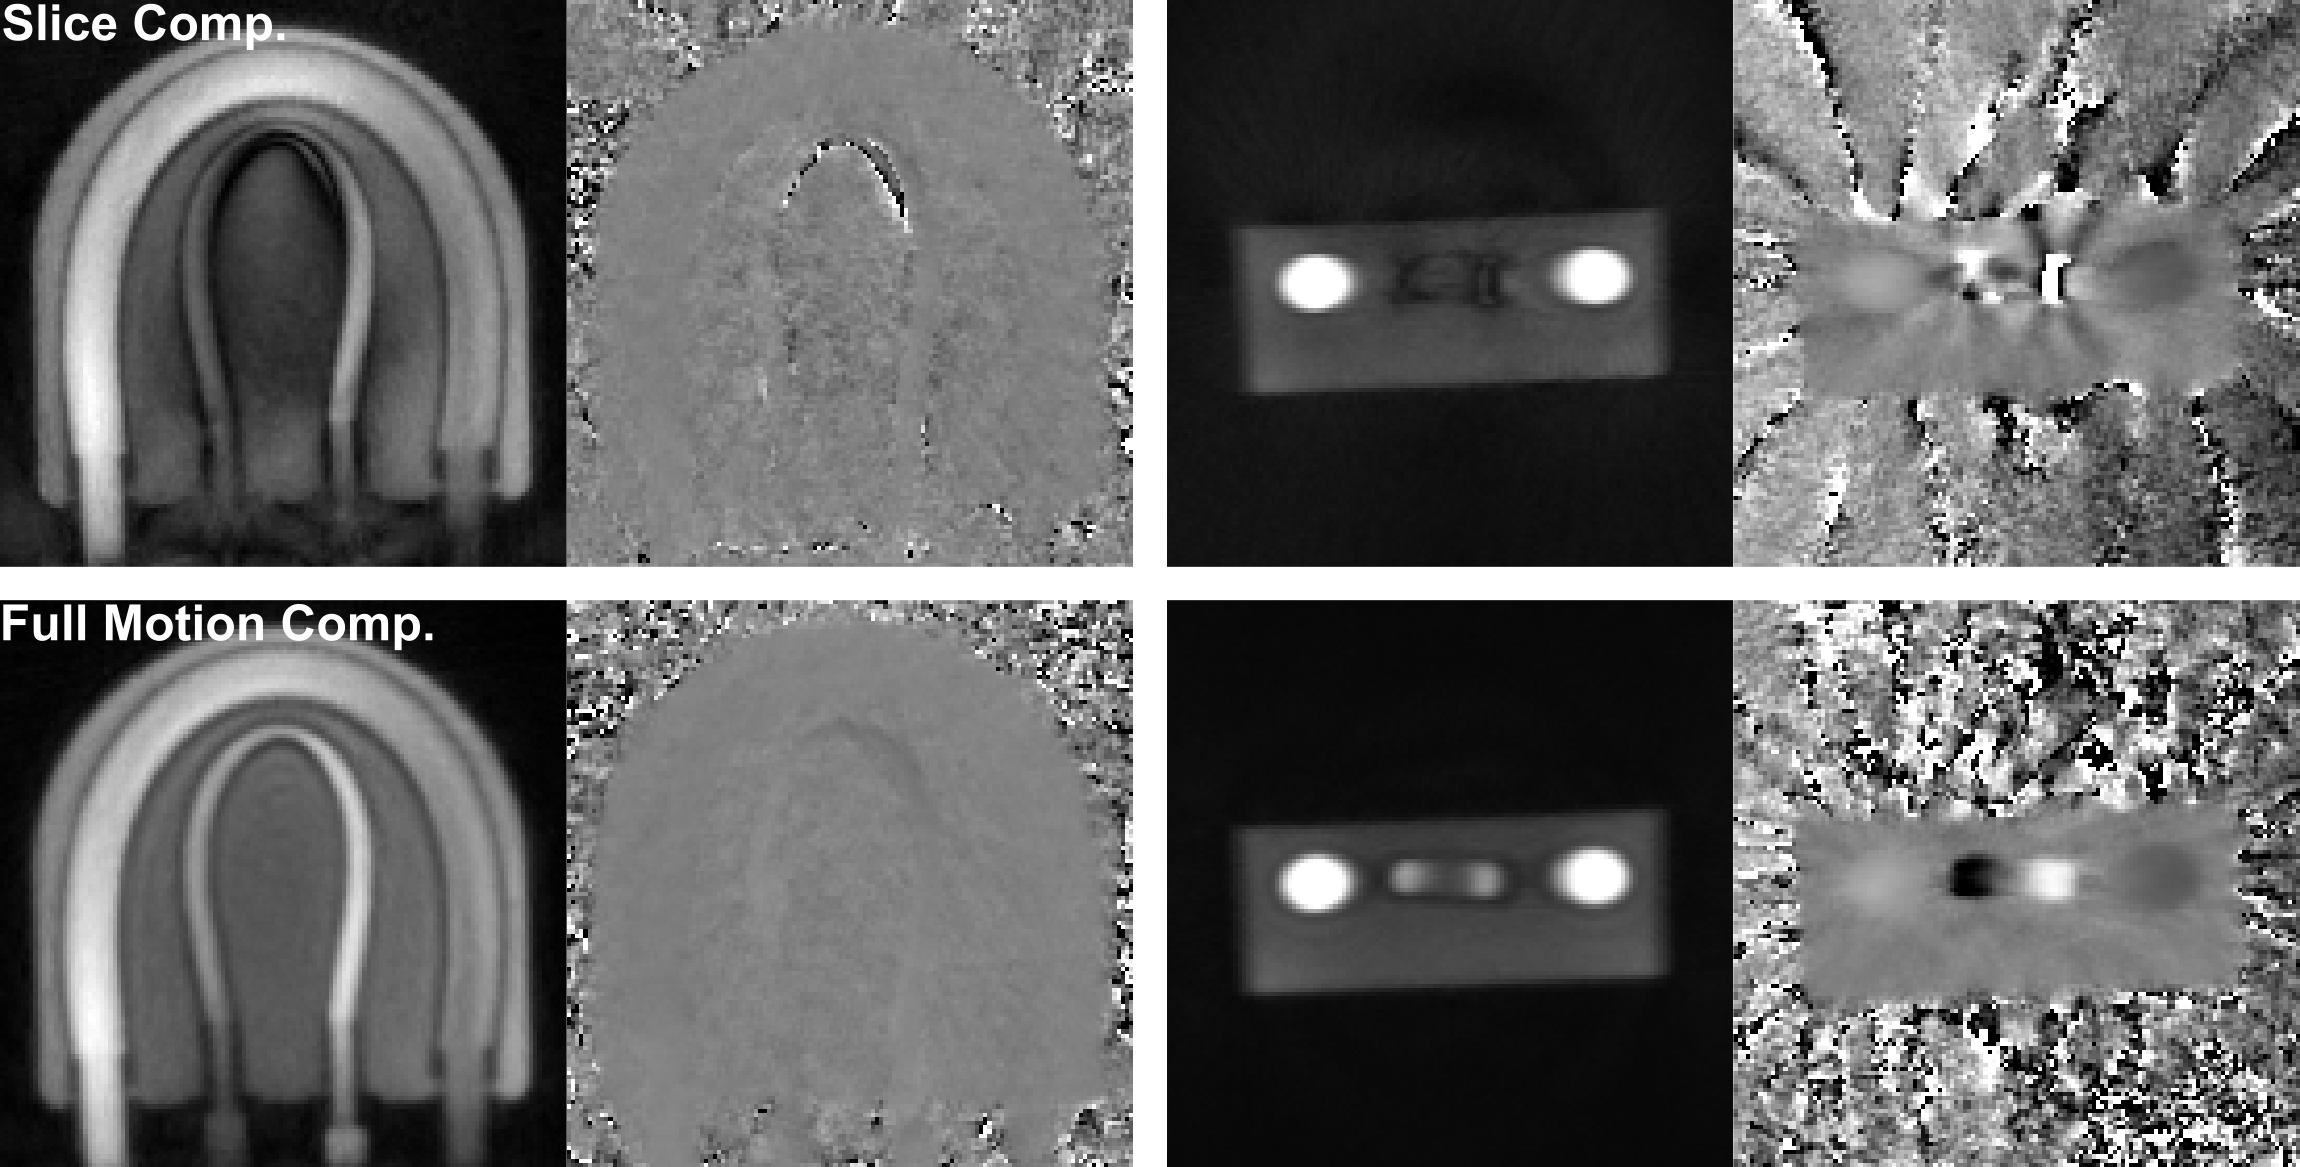
\includegraphics[width=0.80\textwidth]{fig/asym-echo-pha.png}
  \caption{Real-time phase-contrast MRI (\SI{33.3}{\ms} temporal resolution, FOV = \SI{192}{\mm}) of through-plane flow in a phantom with complex flow in the inner small tube. The panels represent selected magnitude images and corresponding phase-contrast maps in a coronal (left) and transverse (right) view at the arch of the inner tube. The images were obtained with velocity-compensating gradient waveforms (top) in slice direction only using symmetric radial gradient echoes and (bottom) in slice and read directions using gradient echoes with \SI{20}{\percent} asymmetry.} \label{Fig:aysm-echo-pha}
  
  \par\bigskip
  
  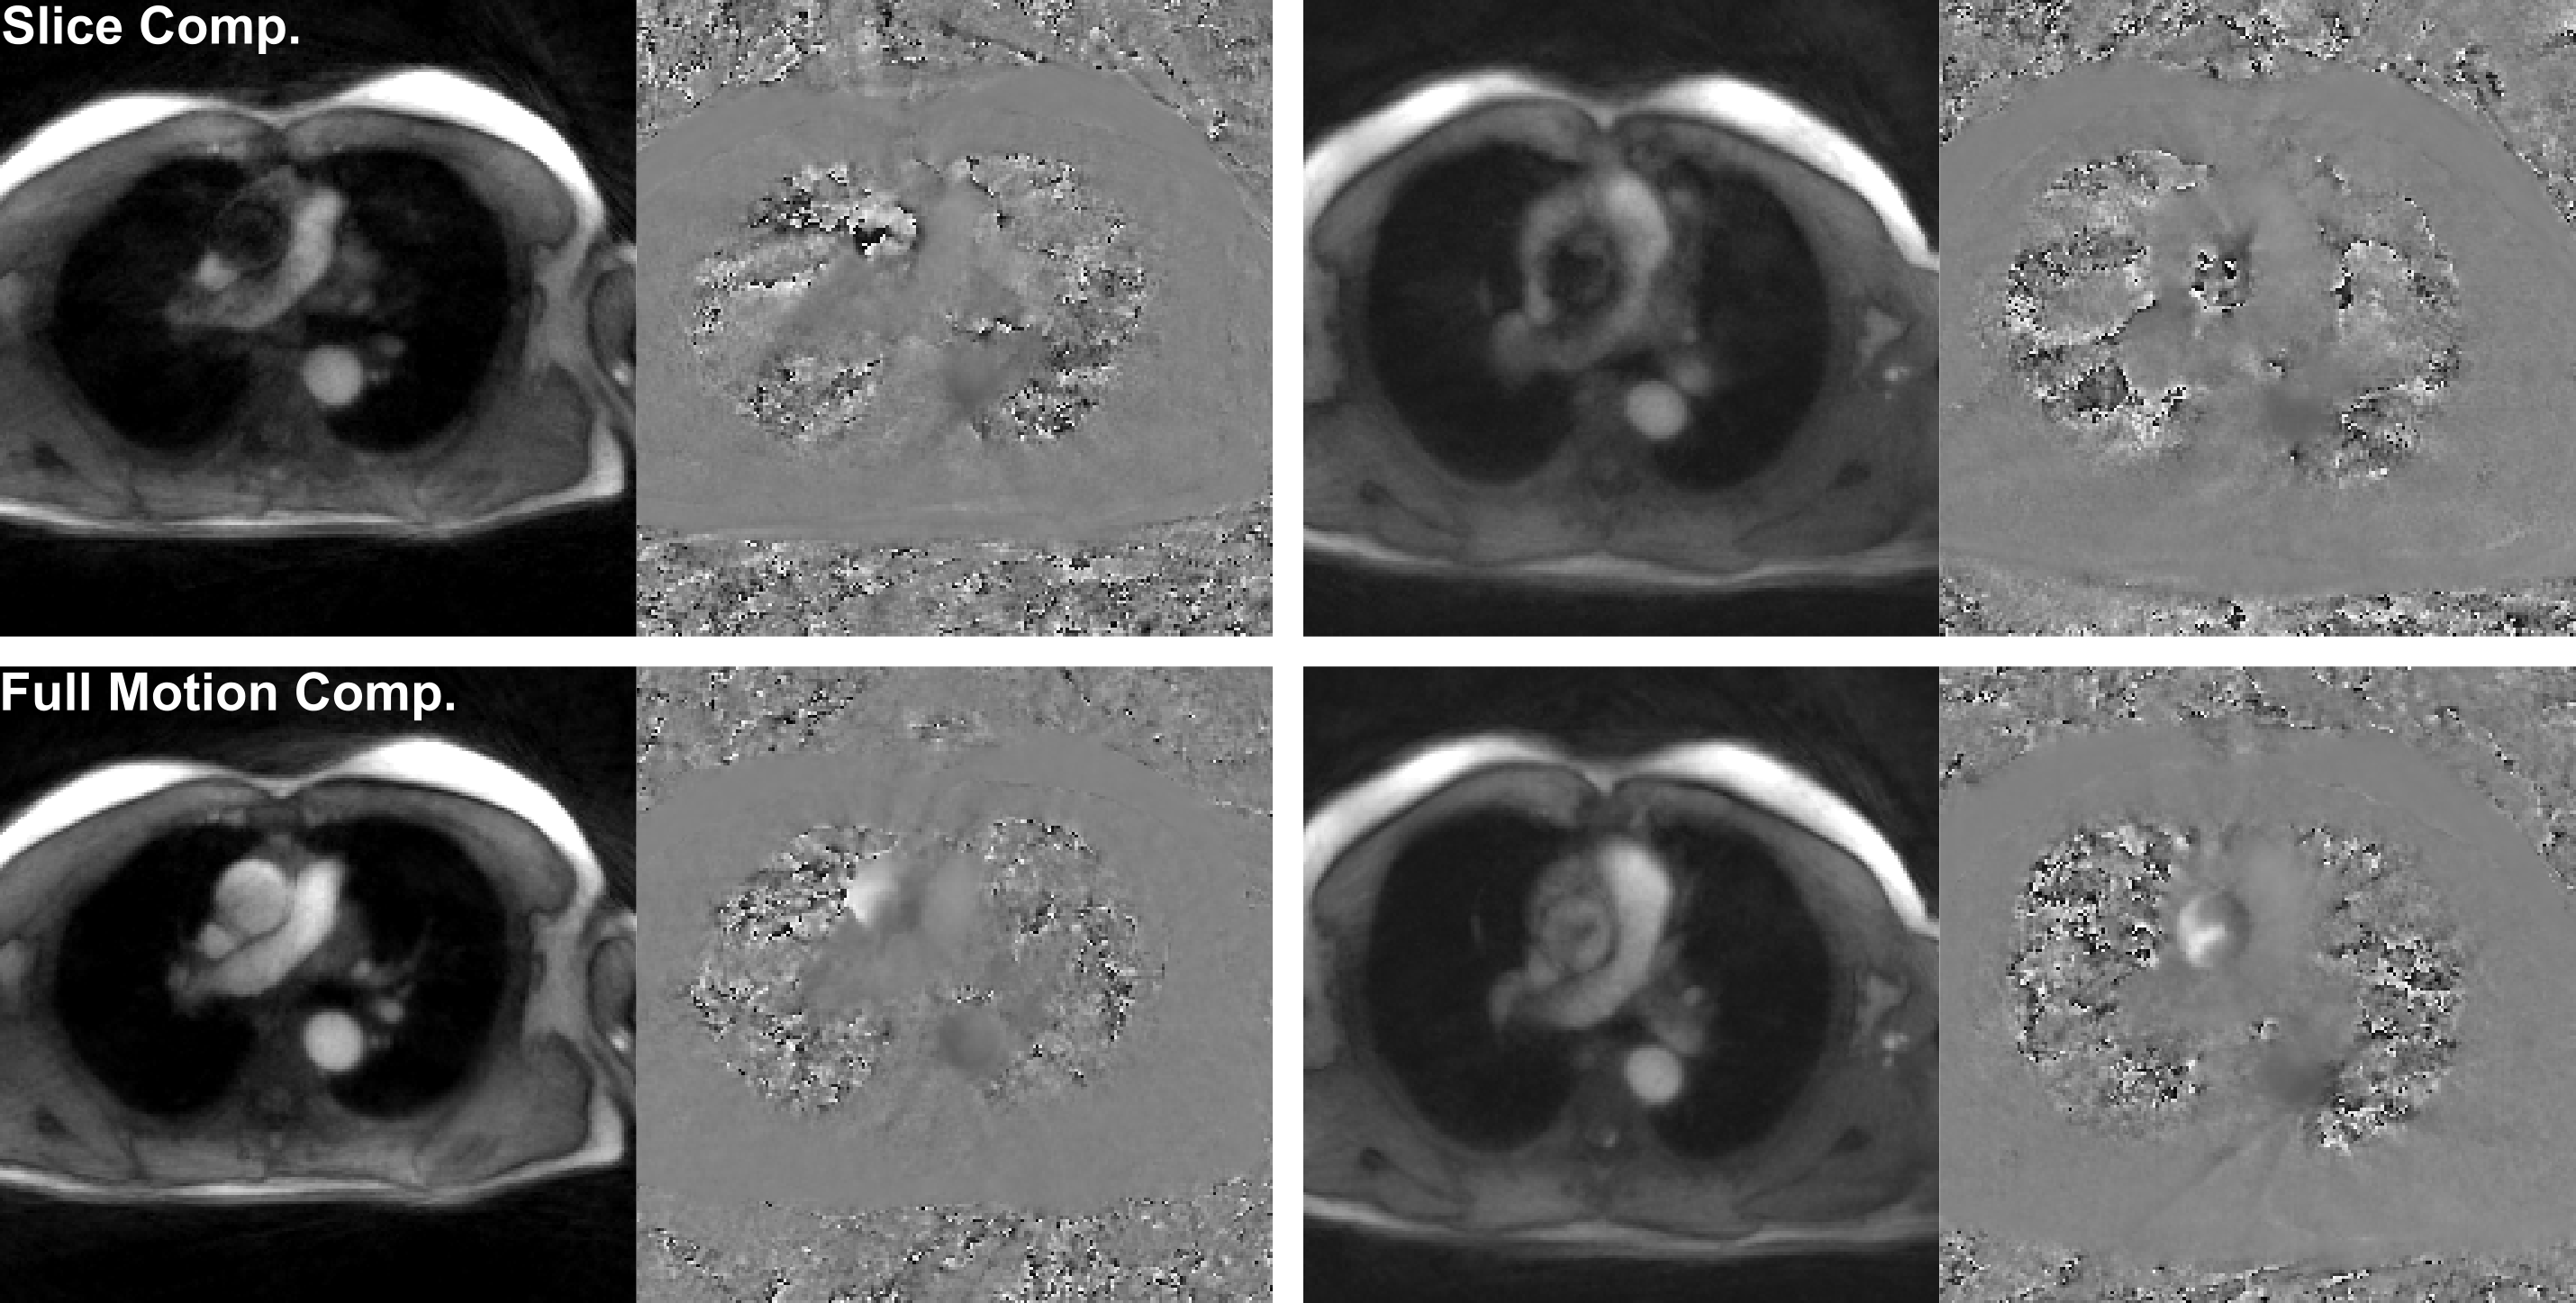
\includegraphics[width=0.80\textwidth]{fig/asym-echo-pat.png}
  \caption{Real-time phase-contrast MRI of aortic blood flow (\SI{35.7}{\ms} temporal resolution, FOV = \SI{320}{\mm}) for a patient with combined aortic valve insufficiency and stenosis. The panels represent selected magnitude images and corresponding phase-contrast maps of the ascending aorta at the level of the pulmonary artery (left) and close to the aortic valve (right). The images were obtained with velocity-compensating gradient waveforms in slice direction only using symmetric radial gradient echoes (top) and in slice and read directions using gradient echoes with \SI{30}{\percent} asymmetry (bottom).} \label{Fig:aysm-echo-pat}
\end{figure}

\begin{table}[tb]
  \caption{Quantitative flow evaluations in the ascending aorta of healthy volunteers and a patient with valve insufficiency\textsuperscript{1}}
  \label{Tab:asym-echo-quant}
  \begin{center}
    \begin{threeparttable}
      \begin{tabular}{ 	c 
                        c 
					    S[table-format=3(2)]
					    S[table-format=3(2)]
					    S[table-format=1.1(2)]
					    S[table-format=2(1)] 
				     }
        \toprule
        \multirow{2}{*}{Subject} & \multirow{2}{*}{MRI} & {Peak Velocity}         & {Flow per}                  & {Flow Volume}          & {Regurgitation}            \\
                                 &                      & {(\si{\cm\per\second})} & {Heartbeat (\si{\milli\L})} & {(\si{\L\per\minute})} & {Fraction (\si{\percent})} \\
		\midrule
        \multirow{3}{*}{No.1}    & {RT-Slice\textsuperscript{2}} & 132\pm7  &  91\pm4 & 5.5\pm0.2 & 2\pm1  \\
                                 & {RT-All\textsuperscript{3}}   & 120\pm3  &  95\pm6 & 5.4\pm0.4 & 2\pm1  \\
                                 & {Cine}                        & 140      & 116     & 7.1       & 1      \\
        \hline
	    \multirow{3}{*}{No.2}    & {RT-Slice}                    & 129\pm9  & 131\pm6 & 7.7\pm0.5 & 1\pm1  \\
	                             & {RT-All}                      & 112\pm9  & 123\pm6 & 6.9\pm0.3 & 1\pm1  \\
	                             & {Cine}                        & 126      & 133     & 7.9       & 1      \\
	    \hline
	    \multirow{3}{*}{No.3}    & {RT-Slice}                    &  76\pm4  &  57\pm4 & 4.0\pm0.2 & 2\pm1  \\
                                 & {RT-All}                      &  69\pm4  &  55\pm1 & 3.6\pm0.2 & 2\pm1  \\
                                 & {Cine}                        &  76      &  65     & 4.3       & 1      \\
	    \hline
	    \multirow{3}{*}{No.4}    & {RT-Slice}                    & 122\pm19 & 126\pm10 & 8.9\pm3.1 & 2\pm1  \\
                                 & {RT-All}                      & 113\pm6  & 121\pm3  & 7.5\pm0.2 & 2\pm1  \\
                                 & {Cine}                        & 117      & 111      & 7.4       & 2      \\
        \hline
   	    \multirow{3}{*}{No.5}    & {RT-Slice}                    & 120\pm8  &  89\pm2  & 5.1\pm0.2 & 5\pm1  \\
                                 & {RT-All}                      & 100\pm6  &  91\pm4  & 5.3\pm0.2 & 5\pm1  \\
                                 & {Cine}                        & 107      & 102      & 6.1       & 4      \\
		\hline
   	    \multirow{2}{*}{Patient} & {RT-All}                      & 260\pm15 &  49\pm7  & 2.7\pm0.5 & 58\pm5  \\
                                 & {Cine}                        & 253      &  50      & 2.6       & 64      \\
	    \bottomrule
      \end{tabular}
  
      \begin{tablenotes}
	    \small
	    \item[1] Results represent mean values $\pm$ standard deviation for \num{10} consecutive heartbeats.
	    \item[2] RT-Slice, real-time flow MRI with velocity compensation in slice direction only.
	    \item[3] RT-All, real-time flow MRI with velocity compensation in slice and read directions.
	  \end{tablenotes}
    \end{threeparttable}
  \end{center}
\end{table}



\subsection{Discussion}
The proposed method for reconstructing highly undersampled asymmetric radial MRI data relies on NLINV \cite{2008_NLINV,2010_NLINV_Heart,2010_20ms_Uecker} with a suitable gradient delay correction. The results obtained for a resolution phantom not only confirm the reliability of the estimated gradient delays for highly undersampled asymmetric echoes, but also demonstrate the achievable image quality and spatial resolution. Only for \SI{20}{\percent} asymmetry the row of \SI{1.5}{\mm} holes in \cref{Fig:aysm-echo-spatialRes} exhibits a slight blurring. This phenomenon reflects the relatively higher fraction of low k-space values in an asymmetric versus a symmetric radial dataset, which for a given weight of the NLINV regularization yields a corresponding overestimation of low spatial frequencies. In principle, the effect may, therefore, be reduced by decreasing the regularization weight which may be accomplished by increasing the number of iterative Gauss-Newton steps used for NLINV reconstruction.

In human studies, complex flow in the ascending aorta with respective multi-dimensional phase contributions is a frequent phenomenon in patients with cardiovascular disease, but not in healthy subjects \cite{2012_PC_Joseph,2014_PC_Joseph}. Nevertheless, a comparison of real-time acquisitions without and with compensation of in-plane phase components reveals approximately \num{10}-\SI{20}{\percent} lower peak flow velocities for later method (see \cref{Tab:asym-echo-quant}). Because velocities directly represent phase information, this observation indicates the successful removal of some false positive phase contributions by the proposed method even in healthy volunteers. In the absence of a gold standard a comparison of these results with those obtained by cine flow MRI are less instructive in view of phase information in real-time acquisitions and the combination of phase information for multiple cardiac cycles in a cine acquisition. However, despite these problems, the flow results obtained for the proposed real-time flow MRI method and the conventional cine MRI method are in general agreement including values for the patient with aortic valve dysfunction.

In conclusion, the development of asymmetric echoes for highly undersampled radial FLASH sequences offers significant technical advances for real-time phase-contrast flow MRI, where the incorporation of velocity compensation in slice and read directions without compromising temporal resolution sets the basis for quantitatively accurate studies. The proposed method now warrants further clinical validation and extensive applications.

\section{Summary}
Asymmetric radial gradient echo sampling has been successfully implemented on the MRI scanner, and the simulated and experimental results reveal a usable degree of up to \SI{20}{\percent} asymmetry. The application of asymmetric echo to real-time phase-contrast flow MRI enables the addition of velocity-compensated gradients without contaminating the temporal resolution. Short echo time and velocity compensation are beneficial in flow velocity measurements as they can decrease phase dispersion and spoil accelerated spins. In addition, asymmetric echo sampling with or without motion compensation can be potentially applied to other applications, i.e., speech studies and cardiac imaging, for the gain of acquisition speed. However, the image reconstruction for asymmetric-echo sampled data is limited to the phase-sensitive NLINV method. The integration of advanced phase constraints into NLINV for extreme asymmetric echo (e.g.~asymmetry $<$ \SI{20}{\percent}) could further reduce echo time, probably recover the missing portion of the asymmetric echo, and eventually improve temporal resolutions of real-time MRI. To implement phase-constrained methods, an appropriate regularization on the phase is most likely required, but the extraction of the phase information from the MR signal model in parallel imaging is complicated and thus requires better mathematical treatments in IRGNM.



\chapter[Model-based Reconstruction for Real-Time Phase-Contrast Flow MRI]
{Model-based Reconstruction \\ 
for Real-Time Phase-Contrast Flow MRI}
\chaptermark{Model-based Phase-Contrast Flow MRI} \label{Chp:mir-pc}

A novel mathematical model of phase-contrast flow MRI is developed based on the assumption that the flow-compensated and flow-encoded images have the same magnitude, but only differ in phases. This assumption is especially true in real-time phase-contrast flow MRI at high temporal resolutions and in conditions where laminar flows are measured. The unknowns (magnitude image, phase-contrast map, and one set of coil sensitivity maps) in this model can be jointly estimated by \acs{IRGNM}. This method avoids the phase-difference calculation and directly applies regularizations on the phase-difference map, which substantially reduces random phase noise.

\section{Introduction}
Based on the physical relationship between a gradient-induced phase shift and the velocity of spins in a corresponding NMR \cite{1960_PC_Hahn} or MRI experiment \cite{1982_PC_Moran} as well as initiated by early seminal applications \cite{1984_PC_Bryant,1984_PC_Dijk,1991_PC_Pelc}, there is nowadays extensive clinical use of velocity-encoded phase-contrast techniques for quantitative MRI studies of blood flow. For relevant reviews see \cite{2005_PC_Gatehouse,2009_PC_Srichai}. More recently, technical advances in real-time MRI \cite{2010_20ms_Uecker}, which rely on regularized NLINV reconstructions of highly undersampled radial gradient-echo acquisitions \cite{2008_NLINV,2010_NLINV_Heart,2012_Schaetz,2014_Temp_Fidelity}, have been extended to cardiovascular applications \cite{2010_RTCMR_Zhang,2013_SSFP_Voit,2014_RT_Zhang} and, in particular, to phase-contrast flow MRI \cite{2012_PC_Joseph,2014_PC_Joseph,2015_PC_Asym}. These and other accelerated flow MRI studies \cite{2005_PC_ktSENSE,2012_PC_Kim} combine parallel imaging with a phase-difference computation \cite{2004_MRI_Bernstein} of two complex images with complementary velocity encodings, i.e., a flow-compensated and a flow-encoded acquisition. As a consequence, phase-difference maps present with extensive phase noise in areas of low or no MRI signal (e.g.~air). Although tolerable in many cases, the presence of strong noise may complicate the definition of the true vessel lumen and therefore affect quantitative flow analyses, hamper the assessment of flow in small vessels or, in case of radial undersampling, enhance residual streaking artifacts. 

On the other hand, model-based approaches in MRI are a well-introduced concept for a variety of post-processing problems, i.e., image segmentation. However, less attention has been paid to model-based reconstructions, despite the fact that respective techniques have previously been detailed in an excellent review \cite{2010_MIR_Fessler}. While selected proposals deal with accelerated $T_2$ mapping \cite{2009_MIR-T2_Block,2011_T2_Sumpf,2014_T2_Sumpf}, fat-water imaging \cite{2004_IDEAL}, inhomogeneity-corrected $T_2^*$ mapping \cite{2009_fim_t2s_me_TMI}, quantitative susceptibility mapping \cite{2013_nlinv_QSM_MRM} and reconstructions of the diffusion tensor \cite{2015_mb_DTI_NBM}, preliminary attempts have also been made to use constrained reconstruction techniques for accelerated phase-contrast flow MRI \cite{2013_PC_CD_Kwak,2015_CD_Sun}. For example, Kwak et al.~\cite{2013_PC_CD_Kwak} reconstructed flow-compensated and flow-encoded images by regularizing the sparsity of the complex-difference image \cite{2004_MRI_Bernstein}.  Alternatively, Sun et al.~\cite{2015_CD_Sun} recently used the complex difference of the acquired raw data in k-space directly as part of a signal model. However, prior to the final calculation of the desired phase-contrast (i.e., velocity) map, both approaches still require the initial reconstruction of either the flow-compensated and flow-encoded image, or the flow-compensated and complex-difference image, and therefore do not offer a direct reconstruction of a phase-contrast velocity map.

In contrast, the present work proposes a model-based reconstruction technique for phase-contrast flow MRI that jointly computes a complex image, a phase-contrast map, and a set of coil sensitivities from every pair of flow-compensated and flow-encoded datasets. In particular, this initial description of a novel technique focuses on real-time flow MRI applications where respective datasets represent extremely undersampled gradient-echo acquisitions \cite{2015_PC_Asym} that allow for monitoring blood flow at very high temporal resolution. Real-time phase-contrast flow MRI thus refers to high-speed MRI acquisitions at millisecond resolution as opposed to ECG-synchronized MRI acquisitions which extend over multiple cardiac cycles. The formulation of the nonlinear inverse reconstruction problem for the proposed signal model leads to an iterative solution which directly offers a quantitatively accurate phase-contrast map with improved spatial accuracy and much reduced phase noise. At this stage, however, and in contrast to a previous real-time phase-contrast flow MRI technique \cite{2015_PC_Asym}, the numerical solution has been developed offline for retrospective analysis.


\section{Algorithm}
\subsection{Phase-Contrast Flow MRI as Nonlinear Inverse Problem}
Assuming the same magnitude image and the same coil sensitivities for each pair ($l=1,2$) of flow-compensated and flow-encoded datasets, the phase-contrast flow MRI signal can be written as
\begin{equation} \label{Equ:signal}
 y_{j,l}(t) = \int_{\vec{r}} \rho(\vec{r}) \cdot e^{z(\vec{r}) \cdot S_l} \cdot c_{j}(\vec{r}) \cdot e^{-i 2\pi \vec{k}_{l}(t) \vec{x}} \text{d}\vec{r} \quad \text{with} \; j \in [1,N], \; l \in [1,2]
\end{equation}
where $\rho$ is the complex image shared by the flow-compensated and the flow-encoding acquisitions, $z$ denotes a complex map which contains the phase differences $\Delta\phi$ in its imaginary part, while the real part is constrained to zero, $c_j$ is the sensitivity map of the $j^{\text{th}}$ coil, and $\vec{k}_{l}$ is the k-space sampling trajectory of the $l^{\text{th}}$ acquisition. The indices $S_1=0$ and $S_2=1$ represent the flow-compensated and the flow-encoded acquisition, respectively. The unknowns ($\rho$, $z$, and $c_j$) in this nonlinear signal model can be solved by IRGNM \cite{1996_regu_inv,2004_iter_inv} as previously introduced for NLINV \cite{2008_NLINV,2010_NLINV_Heart,2010_20ms_Uecker}, which estimates the minimum of the cost function
\begin{equation} \label{Equ:GN_cost}
  \norm{y-F(x)}_2^2 \quad \text{with} \; x = \left( \begin{array}{c} 
  \rho \\
  z \\
  c_1 \\
  \vdots \\
  c_N
  \end{array} \right)
\end{equation}
$x$ the unknowns and $y$ the measured k-space data. According to \cref{Equ:GN_cost}, the forward operator $F$ is
\begin{equation} \label{Equ:GN_fwd}
  F: x \mapsto \left( \begin{array}{c}
  P_1 \mathcal{F} \{\rho \cdot e^{z \cdot 0} \cdot c_1 \} \\
  \vdots \\
  P_1 \mathcal{F} \{\rho \cdot e^{z \cdot 0} \cdot c_N \} \\
  P_2 \mathcal{F} \{\rho \cdot e^{z \cdot 1} \cdot c_1 \} \\
  \vdots \\
  P_2 \mathcal{F} \{\rho \cdot e^{z \cdot 1} \cdot c_N \} \\
  \end{array}  \right)
\end{equation}
with $\mathcal{F}$ the discrete Fourier transform and $P_l$ the orthogonal projection onto the $l^{\text{th}}$ trajectory. In this study, the forward operation on the $j^{\text{th}}$ coil of the $l^{\text{th}}$ acquisition is denoted as: $F_{j,l}(x) = P_l \mathcal{F} \{\rho \cdot e^{z \cdot S_l} \cdot c_j \}$.

Due to the nonlinearity of this forward operator, the iteratively regularized Gauss-Newton method \cite{1996_regu_inv,2004_iter_inv} firstly linearizes the model around the estimate $x_n$ from the $n^{\text{th}}$ Newton step, which yields 
\begin{equation}
  F(x_n + \text{d}x) \approx F(x_n) + DF(x_n) \text{d}x
\end{equation} 
with $DF(x)$ the Frech\'et derivative. Thus, the cost function in \cref{Equ:GN_cost} becomes 
\begin{equation}
  \Phi(\text{d}x) = \norm{[y-F(x_n)] - DF(x_n) \text{d}x}_2^2 \quad ,
\end{equation}
which can be solved with use of the conjugate gradient method. By add Tikhonov regularization similar to \cite{2008_NLINV,2010_NLINV_Heart}, the cost function of linearized model is
\begin{equation} \label{Equ:CG_cost}
  \norm{DF(x_n) \text{d}x-[y-F(x_n)]}_2^2 + \alpha_n \norm{x_n + \text{d}x - p \cdot x_0}_2^2
\end{equation}
with $p$ the damping factor, $\alpha_n$ the Tikhonov regularization parameter which decays in every Newton step, and $x_0$ the initial guess. To solve this problem, two further operators are needed. The first operator is the Frech\'et derivative of the forward operator $DF(x)$, which can be calculated by applying the Jacobian matrix and the linear property of the Fourier transform to $F$. Take $F_{j,l}(x)$ as an example, 
\begin{align} 
  DF_{j,l}(x) \left( \begin{array}{c}
  \text{d} \rho \\
  \text{d} z \\
  \text{d} c_1 \\
  \vdots \\
  \text{d} c_N
  \end{array} \right) 
  &= P_{l} \mathcal{F} \{ e^{z \cdot S_l} \cdot (c_j \cdot \text{d} \rho + S_l \cdot \rho \cdot c_j \cdot \text{d} z + \rho \cdot \text{d} c_j) \} \label{Equ:der} \\
  &= \text{d} y_{j,l} \\
\intertext{where the product of $DF(x)$ and dx maps d$x$ to d$y$. The second operator is the adjoint of the Frech\'et derivative $DF^H (x)$, which can be derived using the unitary property of $\mathcal{F}$,} 
  DF^{H}(x) \left( \begin{array}{c}
  \text{d}y_{1,1} \\
  \vdots \\
  \text{d}y_{N,1} \\
  \text{d}y_{1,2} \\
  \vdots \\
  \text{d}y_{N,2}
  \end{array} \right) 
  &= \left( \begin{array}{c}
  \sum_{j=1}^{N} c_j^* \cdot \big\{ \sum_{l=1}^{2} (e^{z \cdot S_l})^* \cdot \mathcal{F}^{-1} \{P_l^H \text{d}y_{j,l} \} \big\} \\
  \Im \Big( \sum_{j=1}^{N} c_j^* \cdot \big\{ \sum_{l=1}^{2} S_l \cdot (e^{z \cdot S_l})^* \cdot \rho^* \cdot \mathcal{F}^{-1} \{ P_l^H \text{d}y_{j,l} \} \big\} \Big)\\
  \sum_{l=1}^{2} (e^{z \cdot S_l})^* \cdot \rho^* \cdot \mathcal{F}^{-1} \{ P_l^H \text{d}y_{1,l} \} \\
  \vdots \\
  \sum_{l=1}^{2} (e^{z \cdot S_l})^* \cdot \rho^* \cdot \mathcal{F}^{-1} \{ P_l^H \text{d}y_{N,l} \}
  \end{array} \right) \label{Equ:adj}
\end{align}
where $*$ denotes the point-wise complex conjugation and $\Im$ is the imaginary part of d$z$. The imaginary constraint is necessary due to the assumption that the flow-compensated and the flow-encoded datasets only differ in their phases. With the two operators derived above, the solution to \cref{Equ:CG_cost} is
\begin{equation} \label{Equ:CG_sol}
  \text{d}x = [DF(x_n)^H DF(x_n) + \alpha_n I]^{-1} \{ DF(x_n)^H [y-F(x_n)] + \alpha_n (x_0 - x_n) \}
\end{equation}


\subsection{Scaling}
When using first derivatives in a model-based iterative reconstruction of multiple parameters, the relative scaling of parameters should be considered to balance the $L^2$ norm among all partial derivatives. A proper scaling accelerates the iterative optimization process, while maintaining quantitative accuracy, i.e., see \cite{2009_MIR-T2_Block,2011_T2_Sumpf,2014_T2_Sumpf}. For the proposed model-based reconstruction of phase-contrast flow MRI data as proposed here, scaling was accomplished by introducing the scaled index $\hat{S_l}$: $\hat{S_l} = s \cdot S_l$, so that the estimated phase-difference map implicitly becomes 
\begin{equation} \label{Equ:zhat}
  \hat{z} = z / s
\end{equation}
with $s$ being a scalar. From \cref{Equ:adj} the following property can be derived using $\hat{z} \cdot \hat{S_l} = z \cdot S_l$,
\begin{equation} \label{Equ:dz_S}
  \text{d} \hat{z} \propto \hat{S_l}
\end{equation}
Although $s$ may be heuristically selected \cite{2009_MIR-T2_Block}, this work employs an automatic scaling mechanism which takes advantage of \cref{Equ:dz_S} to derive the scaling. It is accomplished by exploiting the complex-difference image \cite{2004_MRI_Bernstein}
\begin{equation} \label{Equ:CD}
  \abs{\rho_1 - \rho_2} = M \cdot \sqrt{2[1-cos(\Delta \phi)]}
\end{equation}
where $M=\abs{\rho_1}=\abs{\rho_2}$. It can then be proven to hold for relatively small phase-differences
\begin{equation} \label{Equ:CD_propto_phi}
  \norm{\sqrt{2 \cdot [1-cos(\Delta \phi)]}}_2 \approx \norm{\Delta \phi}_2
\end{equation}
When normalizing $\rho_1$ and $\rho_2$ by $\norm{M}_2$ and taking the $L^2$ norm of both sides, \cref{Equ:CD}, i.e. the relation between the norm of the complex-difference and that of the phase-difference image, can be reformulated using \cref{Equ:CD_propto_phi}
\begin{equation} \label{Equ:mir_pc_CD_phi}
  \norm{(\rho_1 - \rho_2)/\norm{M}_2}_2 \propto \norm{\Delta \phi}_2
\end{equation}
The norm of the complex-difference in image space is equivalent to that in k-space, so the left-hand side of \cref{Equ:mir_pc_CD_phi} can be estimated from the gridded multi-channel k-space data of the flow-compensated and flow-encoded acquisitions $y_1$ and $y_2$, respectively, 
\begin{equation} \label{Equ:mir_pc_scaling}
  s = \frac{0.5 \cdot (\norm{y_1}_2 + \norm{y_2}_2)}{\norm{y_1 - y_2}_2} \approx \frac{1}{\norm{\Delta \phi}_2} 
\end{equation}
where the scalar $s$ directly quantifies the intensity ratio between the magnitude image and phase-difference map and $1$ indicates the norm of the normalized magnitude image. The scaling mechanism via the scalar $s$ not only balances the derivatives, but also ensures proper balance between the data consistency term and the regularization term in \cref{Equ:CG_cost} because the regularization on $z$ is explicitly controlled by $s$ (see \cref{Equ:zhat}).

\begin{figure}[tb]
  \centering
  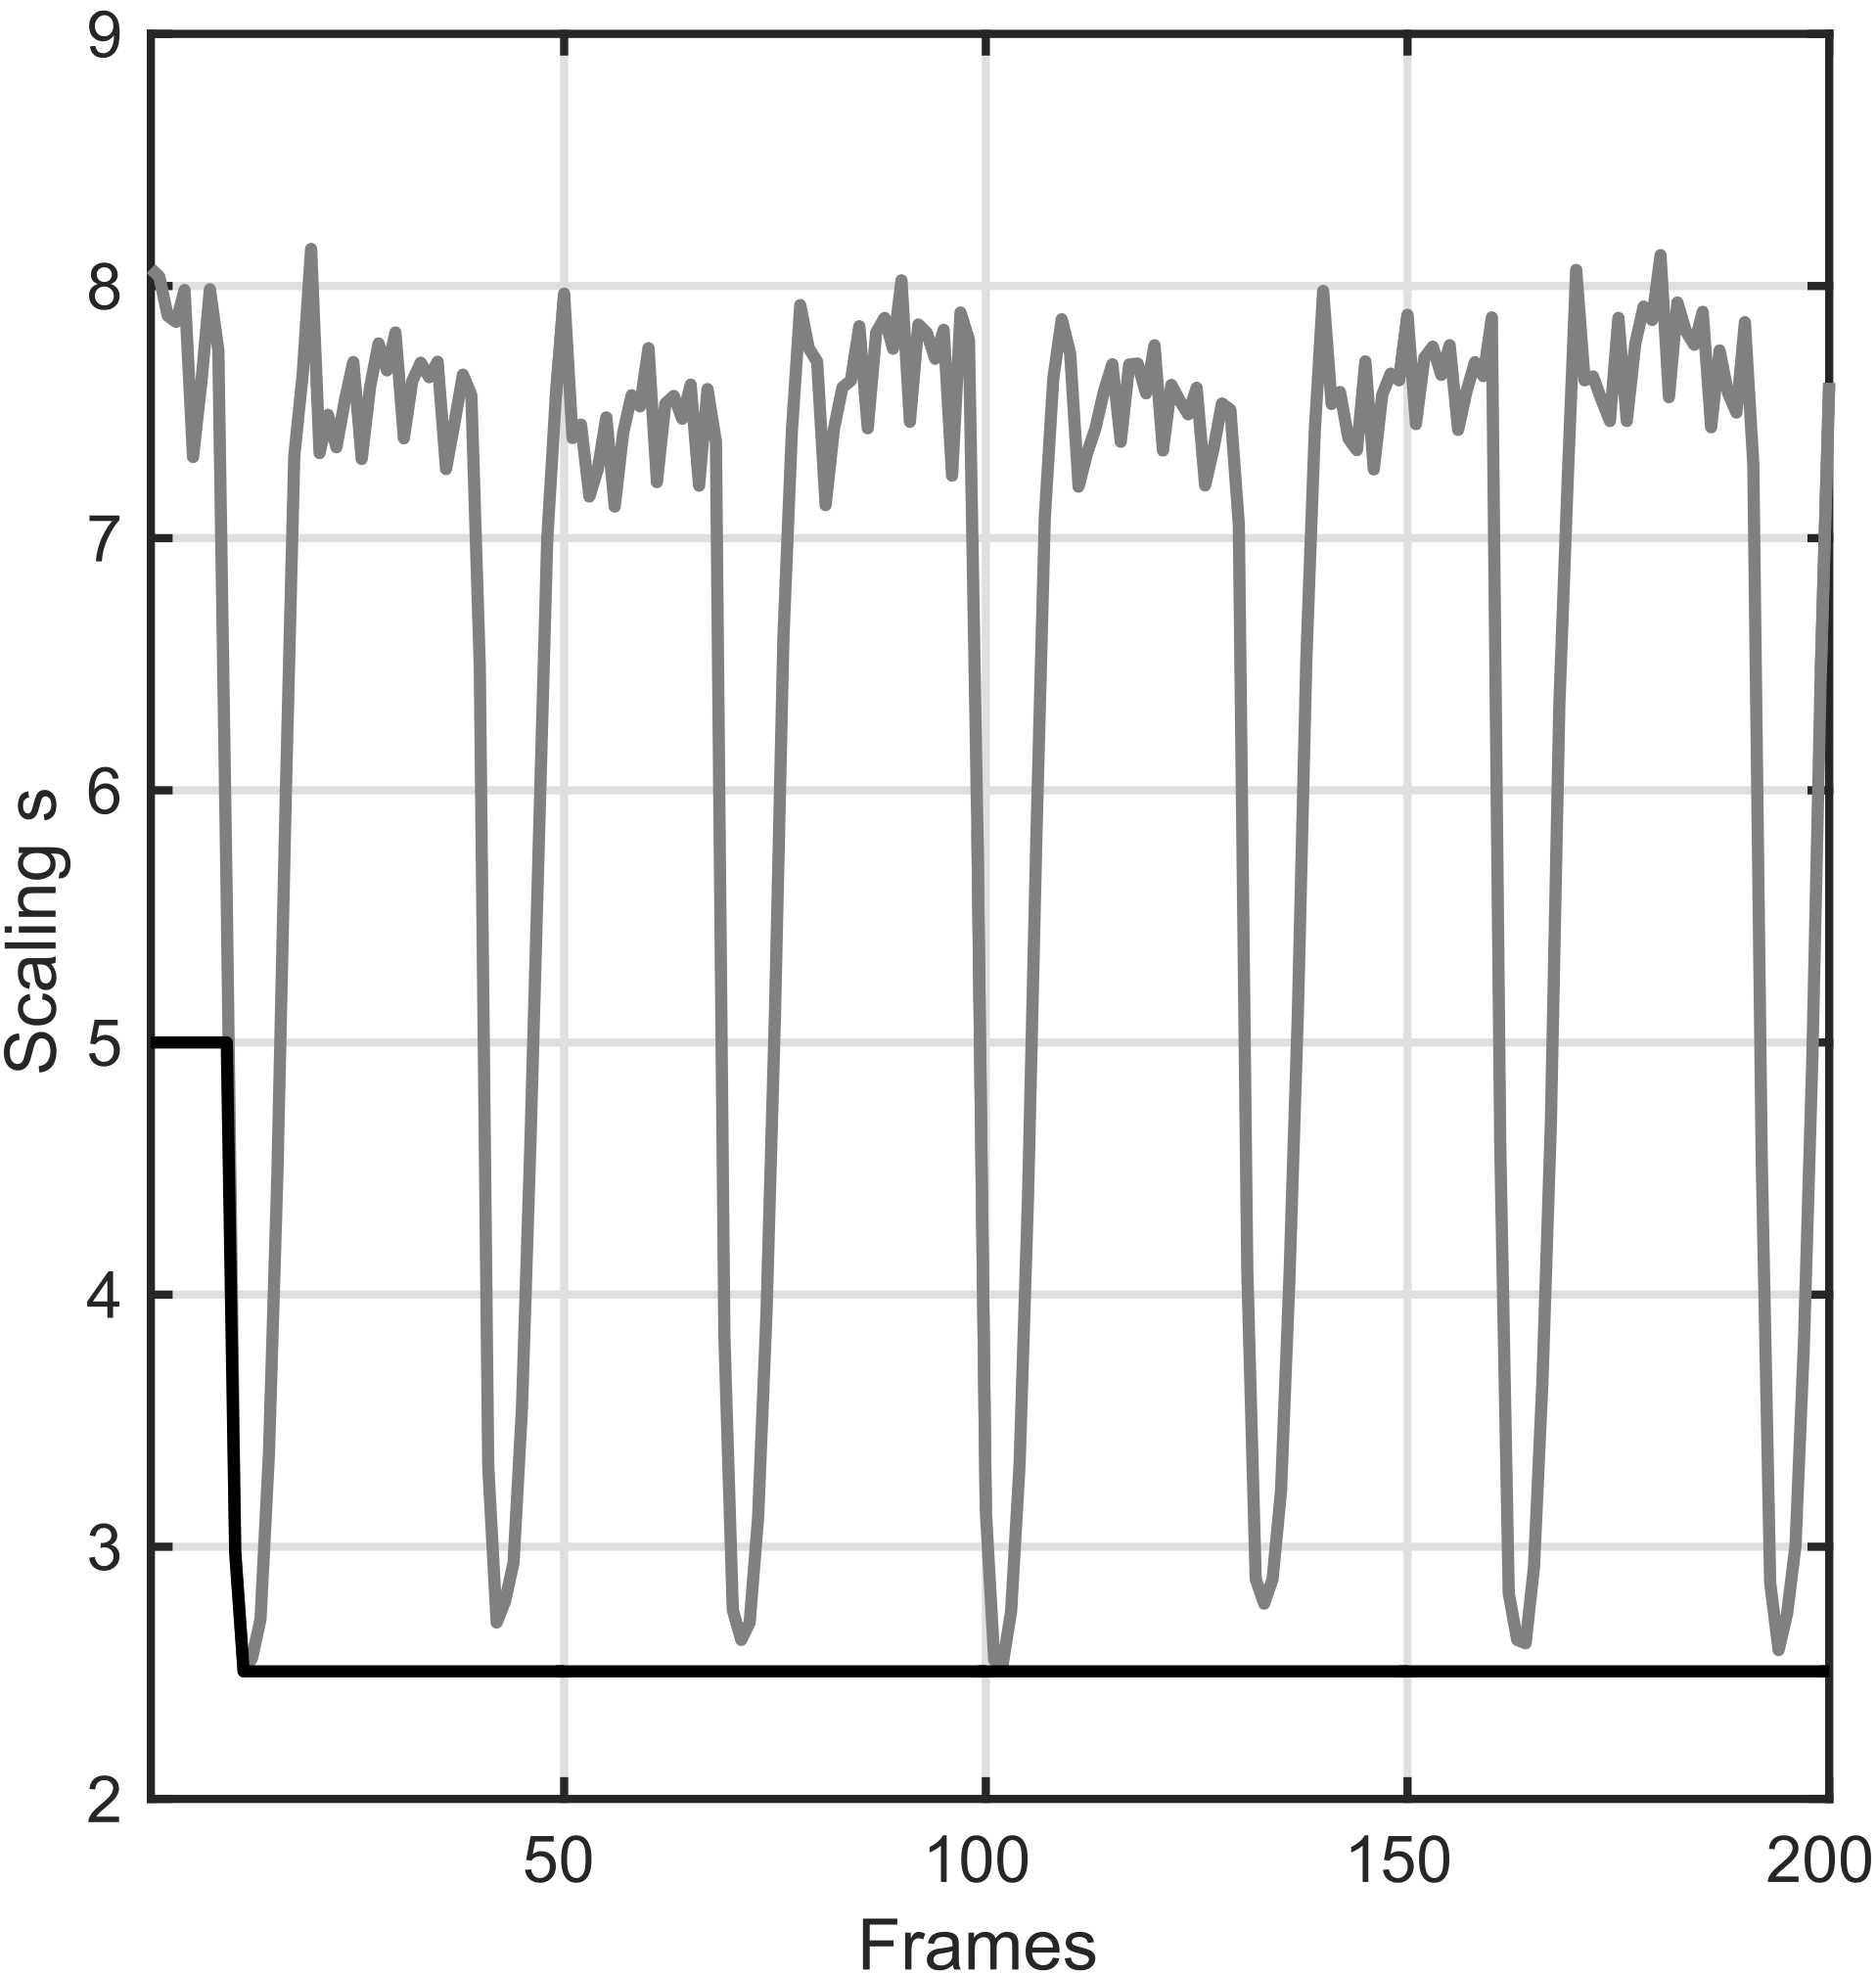
\includegraphics[width=0.8\textwidth]{fig/mir-pc-scaling.png}
  \caption{The scaling values $s$ for real-time phase-contrast flow MRI (\SI{35.7}{\ms} resolution) of the aorta of a healthy subject: Gray line $=$ according to \cref{Equ:mir_pc_scaling}), black line $=$ used for serial model-based reconstructions.} \label{Fig:mir-pc-scaling}
\end{figure}

Because real-time phase-contrast flow MRI is a dynamic process, serial phase-difference maps (as well as complex-difference images) may lead to different scaling values as determined by \cref{Equ:mir_pc_scaling}. This variation is shown in \cref{Fig:mir-pc-scaling} for experimental data of the human aorta (gray line). While $s$ can be as large as \num{10} in case of very low phase-difference values, i.e. in the absence of flow, such large values should be avoided as they decrease the regularization strength and accumulate noise in the final estimate. Therefore, the following steps are taken to dynamically determine the effective scaling. Starting with a value of \num{5}, $s$ is calculated from \cref{Equ:mir_pc_scaling} for each frame and continuously updated by any lower scaling. For studies of human blood flow this typically means that $s$ decreases until the real-time flow MRI acquisition reaches the first systole (compare \cref{Fig:mir-pc-scaling}, black line), so that quantitative analyses of real-time flow MRI studies may eliminate the first cardiac cycle.


\subsection{Regularization}
As shown in \cref{Equ:CG_cost}, Tikhonov regularization is used for the solution of the linear problem with $\alpha_n$ a tunable regularization parameter, which starts with \num{1} and decreases in each Newton step by a factor of \num{2}. In this study, $\alpha_n$ is identical among all parameters. In addition, the model-based image reconstruction adopts the $L^2$-norm regularization on the high spatial frequencies of the coil sensitivity maps as used for NLINV \cite{2010_20ms_Uecker,2008_NLINV,2010_NLINV_Heart,2012_PC_Joseph,2014_PC_Joseph,2015_PC_Asym}, and employs a temporal regularization of the current set of model parameters (i.e., maps) with the respective maps of the immediately preceding pair of datasets damped by \num{0.7}. The reconstruction on the very first maps is initialized using $\rho=1$, $z=0$, and $c_j=0$, and \num{7} Newton steps are used in this work.

The radial sampling pattern has a circular field-of-view, and thus encodes no information in the corners of k-space. As a result, high spatial-frequency signal, which usually appears as checkerboard artifacts in image domain, has the freedom to accumulate during model-based iterative reconstruction. Therefore, a k-space filter \cite{2001_gSENSE} is added to the gridded sampling pattern P to penalize signals in the undefined corners of k-space.


\subsection{Pre- and Post-Processing}
In general, the datasets from multiple receiver coils are first corrected for gradient delay errors \cite{2015_PC_Asym}, and then compressed to \num{10} virtual coils by a principle component analysis. This latter process must be identical for both the flow-compensated and flow-encoded datasets. Finally, the data and the sampling trajectories are interpolated onto Cartesian grids without density compensation. After solving the nonlinear inverse problem, the resulting complex phase-contrast map is given by
\begin{equation} \label{Equ:post_PC}
  \rho_{PC} = \abs{\rho} \cdot e^{i \cdot s \cdot \Im(\hat{z})} \quad .
\end{equation}


\section{Methods}
\subsection{Numerical Flow Phantom}
To ensure the quantitative accuracy of the proposed reconstruction method, a numerical flow phantom was built with superimposed ellipses, whose analytical Fourier transform is known and can be evaluated at given k-space trajectories. Moreover, \num{10} receiver coils were simulated based on the Biot-Savart law and sinusoidal fitting \cite{2012_analSim}. To mimic phase-contrast flow MRI, the simulation included one flow-compensated and one flow-encoded acquisition with the same magnitude signal strengths. The simulated ellipses had zero phase in the flow-compensated acquisition, while phase values of \SI{150}{\degree}, \SI{-100}{\degree}, and \SI{-15}{\degree} were added to the three ellipses in the flow-encoded acquisition to represent different velocities and directions. The simulations were performed for datasets with \num{45}, \num{15}, \num{7} and \num{5} radial spokes (symmetric echoes, base resolution \num{170} pixels) each covering a view angle of \SI{360}{\degree}. Serial datasets employed interleaved spokes in \num{5} successive acquisitions similar to experimental conditions. Complex white Gaussian noise with a standard deviation of \num{0.1} was added to the data, so that the signal-to-noise ratio decreased with the number of spokes. While model-based image reconstructions of numerical phantoms which are based on analytical Fourier transform usually suffer from aliasing artifacts, these may be suppressed by decreasing the Tikhonov regularization parameter or by adjusting the sampling pattern \cite{2011_T2_Sumpf}. Here, a damping factor of \num{1} for the $z$ map was only used for reconstructions of the numerical flow phantom.


\subsection{Real-Time Phase-Contrast Flow MRI}
This work presents real-time flow MRI data of the ascending (and descending) aorta obtained at \SI{3}{\tesla} (Magnetom Prisma, Siemens Healthcare, Erlangen, Germany). The analyses include \num{5} volunteers without known illness and two patients with combined aortic valve insufficiency and partial stenosis previously studied with “conventional” real-time flow MRI \cite{2015_PC_Asym} as well as new experimental data from 5 additional healthy subjects. All subjects gave written informed consent prior to MRI in compliance with the regulations established by the local ethics committee. 

Real-time phase-contrast flow MRI was based on extremely undersampled radial FLASH MRI (\num{5} or \num{7} spokes per image) with asymmetric gradient echoes \cite{2015_PC_Asym} using two sequential acquisitions of a dataset with velocity-compensated gradients in all gradient axes and with velocity-encoding of through-plane flow, respectively. While studies of the experimental flow phantom ($\text{VENC} = \SI[per-mode=reciprocal]{200}{\cm\per\second}$) employed the 64-channel head coil, blood flow in the human aorta ($\text{VENC} = 200\text{ to }\SI{400}{\cm\per\second}$) was studied during free breathing by combining an 18-element thorax coil with 32 elements of the spine coil. Acquisitions (TR/TE = \num{2.38}/\SI{1.59}{\ms}, flip angle \SI{10}{\degree}) of the previously described flow phantom \cite{2015_PC_Asym} were performed at \SI{1.4}{\mm} in-plane resolution (\SI{192}{\mm} field-of-view, \SI{6}{\mm} slice thickness) and \SI{33.32}{\ms} temporal resolution (\num{7} spokes for the flow-encoded and flow-compensated image, respectively). All in vivo measurements (TE = \SI{1.70}{\ms}, flip angle \SI{10}{\degree}) had \SI{1.5}{\mm} in-plane resolution, \SI{320}{\mm} field-of-view, \SI{6}{\mm} slice thickness, and \SI{35.7}{\ms} (\num{2 x 7} spokes, TR = \SI{2.55}{\ms}) or \SI{25.6}{\ms} temporal resolution (\num{2 x 5} spokes, TR = \SI{2.56}{\ms}) corresponding to \num{28} or \num{39} frames per second (fps), respectively. For both NLINV and model-based reconstructions the serial magnitude images were subject to a temporal median filter, whereas no temporal filter was applied to phase-contrast maps. 

Online reconstruction and display of real-time NLINV images was achieved by a parallelized version of the NLINV algorithm \cite{2012_Schaetz} and a bypass computer (sysGen/TYAN Octuple-\acs{GPU}, Sysgen, Bremen, Germany) equipped with two processors (CPU, SandyBridge E5-2650, Intel, Santa Clara, CA) and \num{8} graphics processing units (TITAN, NVIDIA, Santa Clara, CA). The system was fully integrated into the reconstruction pipeline of the commercial MRI system. Depending on image matrix (i.e., resolution and/or FOV) the current reconstruction speed ranges from \num{6} to \num{14} fps (i.e., magnitude images and phase-contrast maps). At this stage, the model-based reconstruction was implemented on a single graphics processing unit (GeForce GTX 580, NVIDIA, Santa Clara, CA) and performed offline after data acquisitions. Typically, the current implementation takes about \SI{4.5}{\second} per frame.

Quantitative analyses of phase-contrast flow MRI data were obtained with the use of CAIPI prototype software (Fraunhofer MEVIS, Bremen, Germany), especially modified for the automated analysis of real-time MRI data, i.e., vessel or myocardial segmentation throughout the entire time series without the need for manual corrections \cite{2014_img_segment}.

\clearpage


\section{Results}
\subsection{Validation Studies}
In order to assess the quantitative reliability of the model-based phase-contrast flow MRI technique, the mathematical approach was validated with the use of a numerical flow phantom providing ground truth in the presence of noise. \cref{Fig:mir-pc-sim-pha} compares the results obtained for NLINV reconstructions with subsequent calculation of a phase-difference map and direct model-based reconstructions for simulations with a decreasing number of spokes per image. For high degrees of undersampling, the model-based phase-contrast maps present with visibly better signal-to-noise ratio and sharper “vessel” definition. The quantitative analyses in \cref{Tab:mir-pc-sim-pha} confirm the excellent accuracy of phase (i.e., velocity) values obtained by the proposed model-based reconstruction – even for acquisitions with only \num{7} or \num{5} spokes per image. Most importantly, this not only applies to mean values, but also to the standard deviations which for highly undersampled acquisitions are much smaller than for NLINV-based reconstructions.

Similarly, \cref{Fig:mir-pc-exp-pha} shows the results for an experimental phantom providing constant flow at two different velocities (i.e., depending on tube diameter) and two opposing flow directions (forward vs backward flow). Again, the most apparent feature is the almost noise-less appearance of the model-based phase-contrast map which benefits from the a priori knowledge of zero phase for all pixels without flow or no MRI signal. In contrast, all “conventional” flow MRI techniques, which rely on the phase-difference calculation of two independent complex images with differential flow encodings, yield arbitrary phase values (and corresponding phase differences) in zero-signal pixels as well as some tissue-dependent phase in pixels with stationary signal. In relation to this advantageous zero-phase property, which is effective as an additional constraint, the model-based reconstruction reduces the strength of residual streakings extending from the high-flow tubes in the phase-contrast maps shown in \cref{Fig:mir-pc-exp-pha}.

Most importantly, however, model-based phase-contrast maps yield a spatially much more accurate definition of the flow signal (i.e., vessel lumen) than obtainable by conventional NLINV reconstructions. In fact, the spatial information of the model-based phase-contrast map in \cref{Fig:mir-pc-exp-pha} precisely matches the magnitude image information, whereas flow areas in NLINV phase-contrast maps are larger compared to both the true lumen sizes. These qualitative observations are confirmed by quantitative analyses summarized in \cref{Tab:mir-pc-exp-pha}. In contrast to NLINV, model-based reconstructions not only yield almost identical flow areas in magnitude images and phase-contrast maps, but are also in close agreement with estimates of tube sizes as obtained by high-resolution MRI. Nevertheless, flow evaluations reveal good agreement between both flow MRI methods with respect to peak velocity as a direct (though focal) result of the phase-contrast determination, while flow volumes tend to be slightly larger than a determination by a flow meter.
\vspace{10mm}

\begin{figure}[h!]
  \centering
  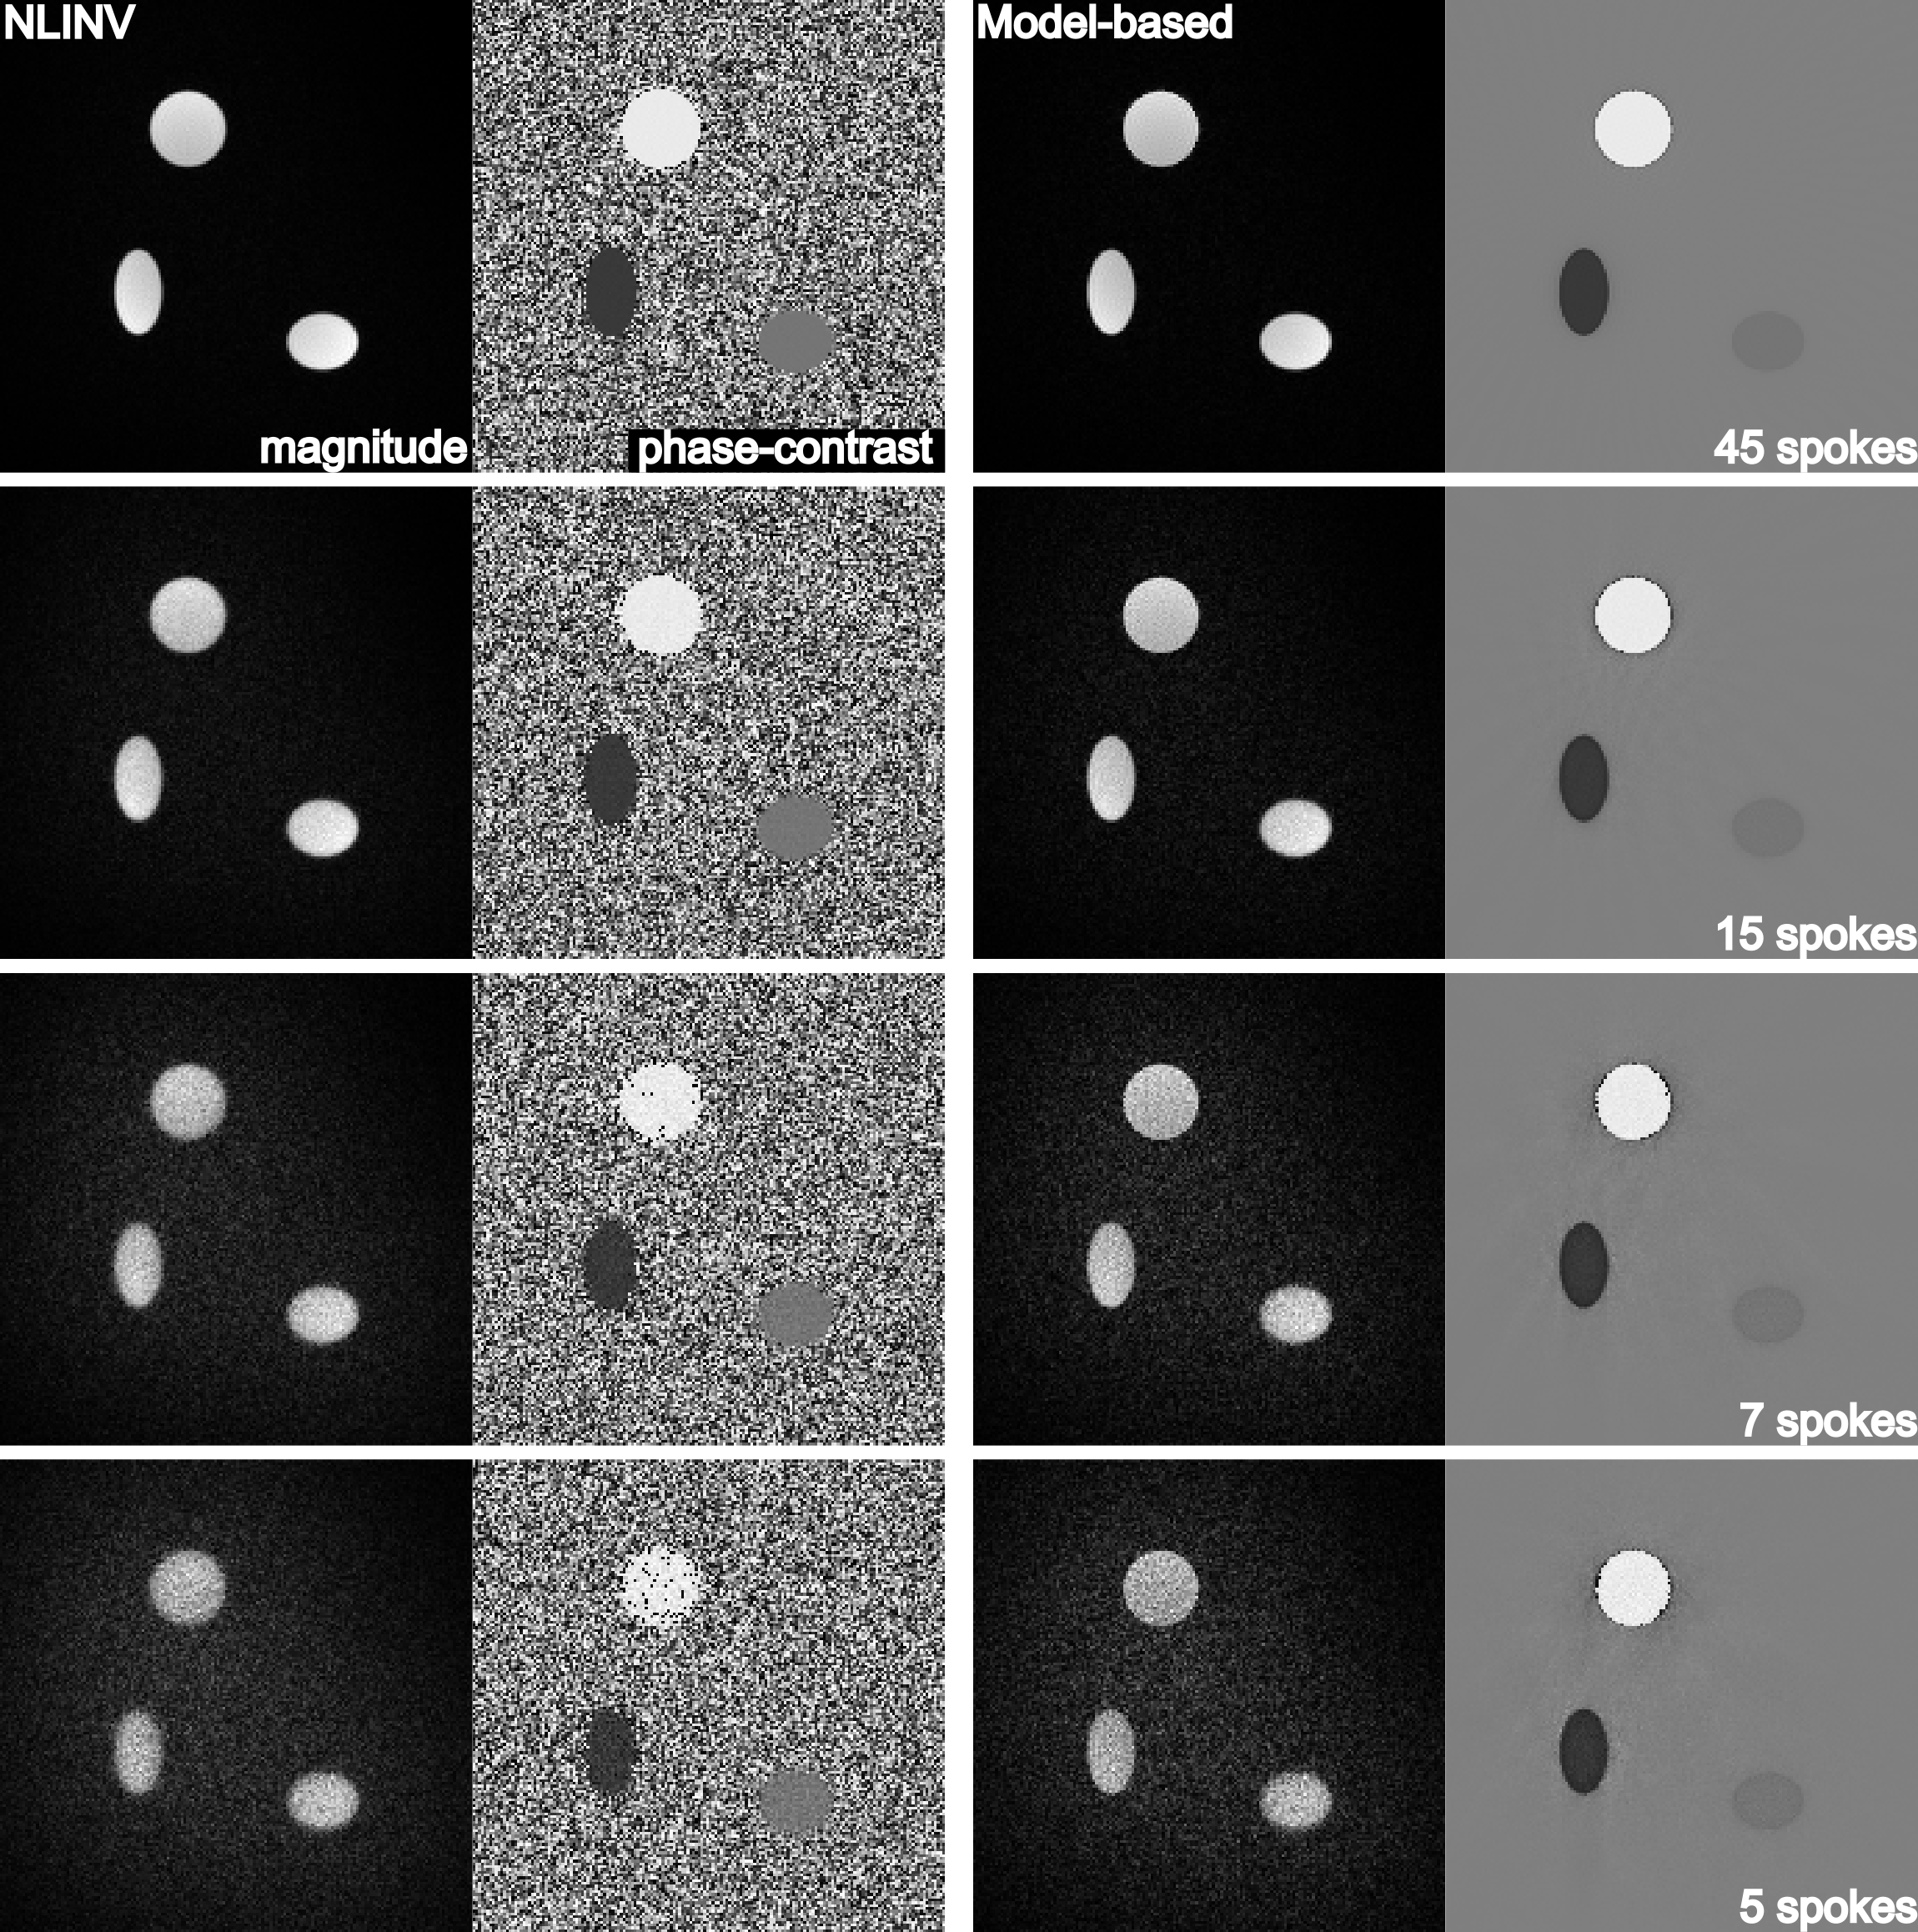
\includegraphics[width=\textwidth]{fig/mir-pc-sim-pha.png}
  \caption{(Left) NLINV and (right) model-based reconstructions of magnitude images and phase-contrast maps for a numerical flow phantom (complex white Gaussian noise, standard deviation \num{0.1}) and constant flow in three ellipses corresponding to phase values of \ang{150}, \ang{-100}, and \ang{-10}. The results were obtained for simulated acquisitions with \num{45}, \num{15}, \num{7} and \num{5} spokes. The Gibbs ringing artifact around the \ang{150} ellipse in phase-contrast maps stems from the numerical design of the phantom (plug flow pattern). It is less visible in NLINV reconstructions because of the phase noise for zero-flow pixels.} \label{Fig:mir-pc-sim-pha}
\end{figure}

\begin{table}[tb]
  \caption{Quantitative flow evaluations for a numerical flow phantom}
  \label{Tab:mir-pc-sim-pha}
  \begin{center}
    \begin{threeparttable}
      \begin{tabular}{ 	c 
					    S[table-format=-3]
					    S[table-format=-3.1(2)]
					    S[table-format=-3.1(2)] 
				     }
        \toprule
        {Spokes per image} & {True Phase Difference} & {NLINV\textsuperscript{1}} & {Model-based\textsuperscript{2}} \\
		\midrule
        \multirow{3}{*}{\tablenum[table-format=2]{45}} & 150  & 150.0\pm1.7   & 150.1\pm1.4  \\
                                                       & -100 & -100.0\pm1.4  & -100.2\pm1.0 \\
                                                       & -15  & -15.0\pm1.3   & -15.1\pm0.6  \\
        \hline
	    \multirow{3}{*}{\tablenum[table-format=2]{15}} & 150  & 150.0\pm5.5   & 149.8\pm2.5  \\
		                                               & -100 & -100.0\pm5.2  & -100.2\pm2.3 \\
		                                               & -15  & -15.0\pm4.4   & -15.0\pm1.6  \\
	    \hline
		\multirow{3}{*}{\tablenum[table-format=2]{7}}  & 150  & 146.4\pm36.0  & 149.6\pm5.7  \\
	                                                   & -100 & -100.8\pm12.0 & -102.7\pm5.3 \\
	                                                   & -15  & -15.6\pm10.6  & -15.5\pm3.1  \\
	    \hline
	    \multirow{3}{*}{\tablenum[table-format=2]{5}}  & 150  & 131.7\pm73.8  & 150.6\pm8.8  \\
		                                               & -100 & -101.6\pm18.6 & -103.8\pm6.5 \\
		                                               & -15  & -15.4\pm14.5  & -15.9\pm3.7  \\
	    \bottomrule
      \end{tabular}
  
      \begin{tablenotes}
	    \small
	    \item Results represent mean values $\pm$ standard deviations.
	    \item[1] NLINV reconstructions with subsequent calculation of a phase-different map.
	    \item[2] Direct model-based reconstruction of phase-contrast map.
	  \end{tablenotes}
    \end{threeparttable}
  \end{center}
\end{table}


\begin{figure}[tb]
  \centering
  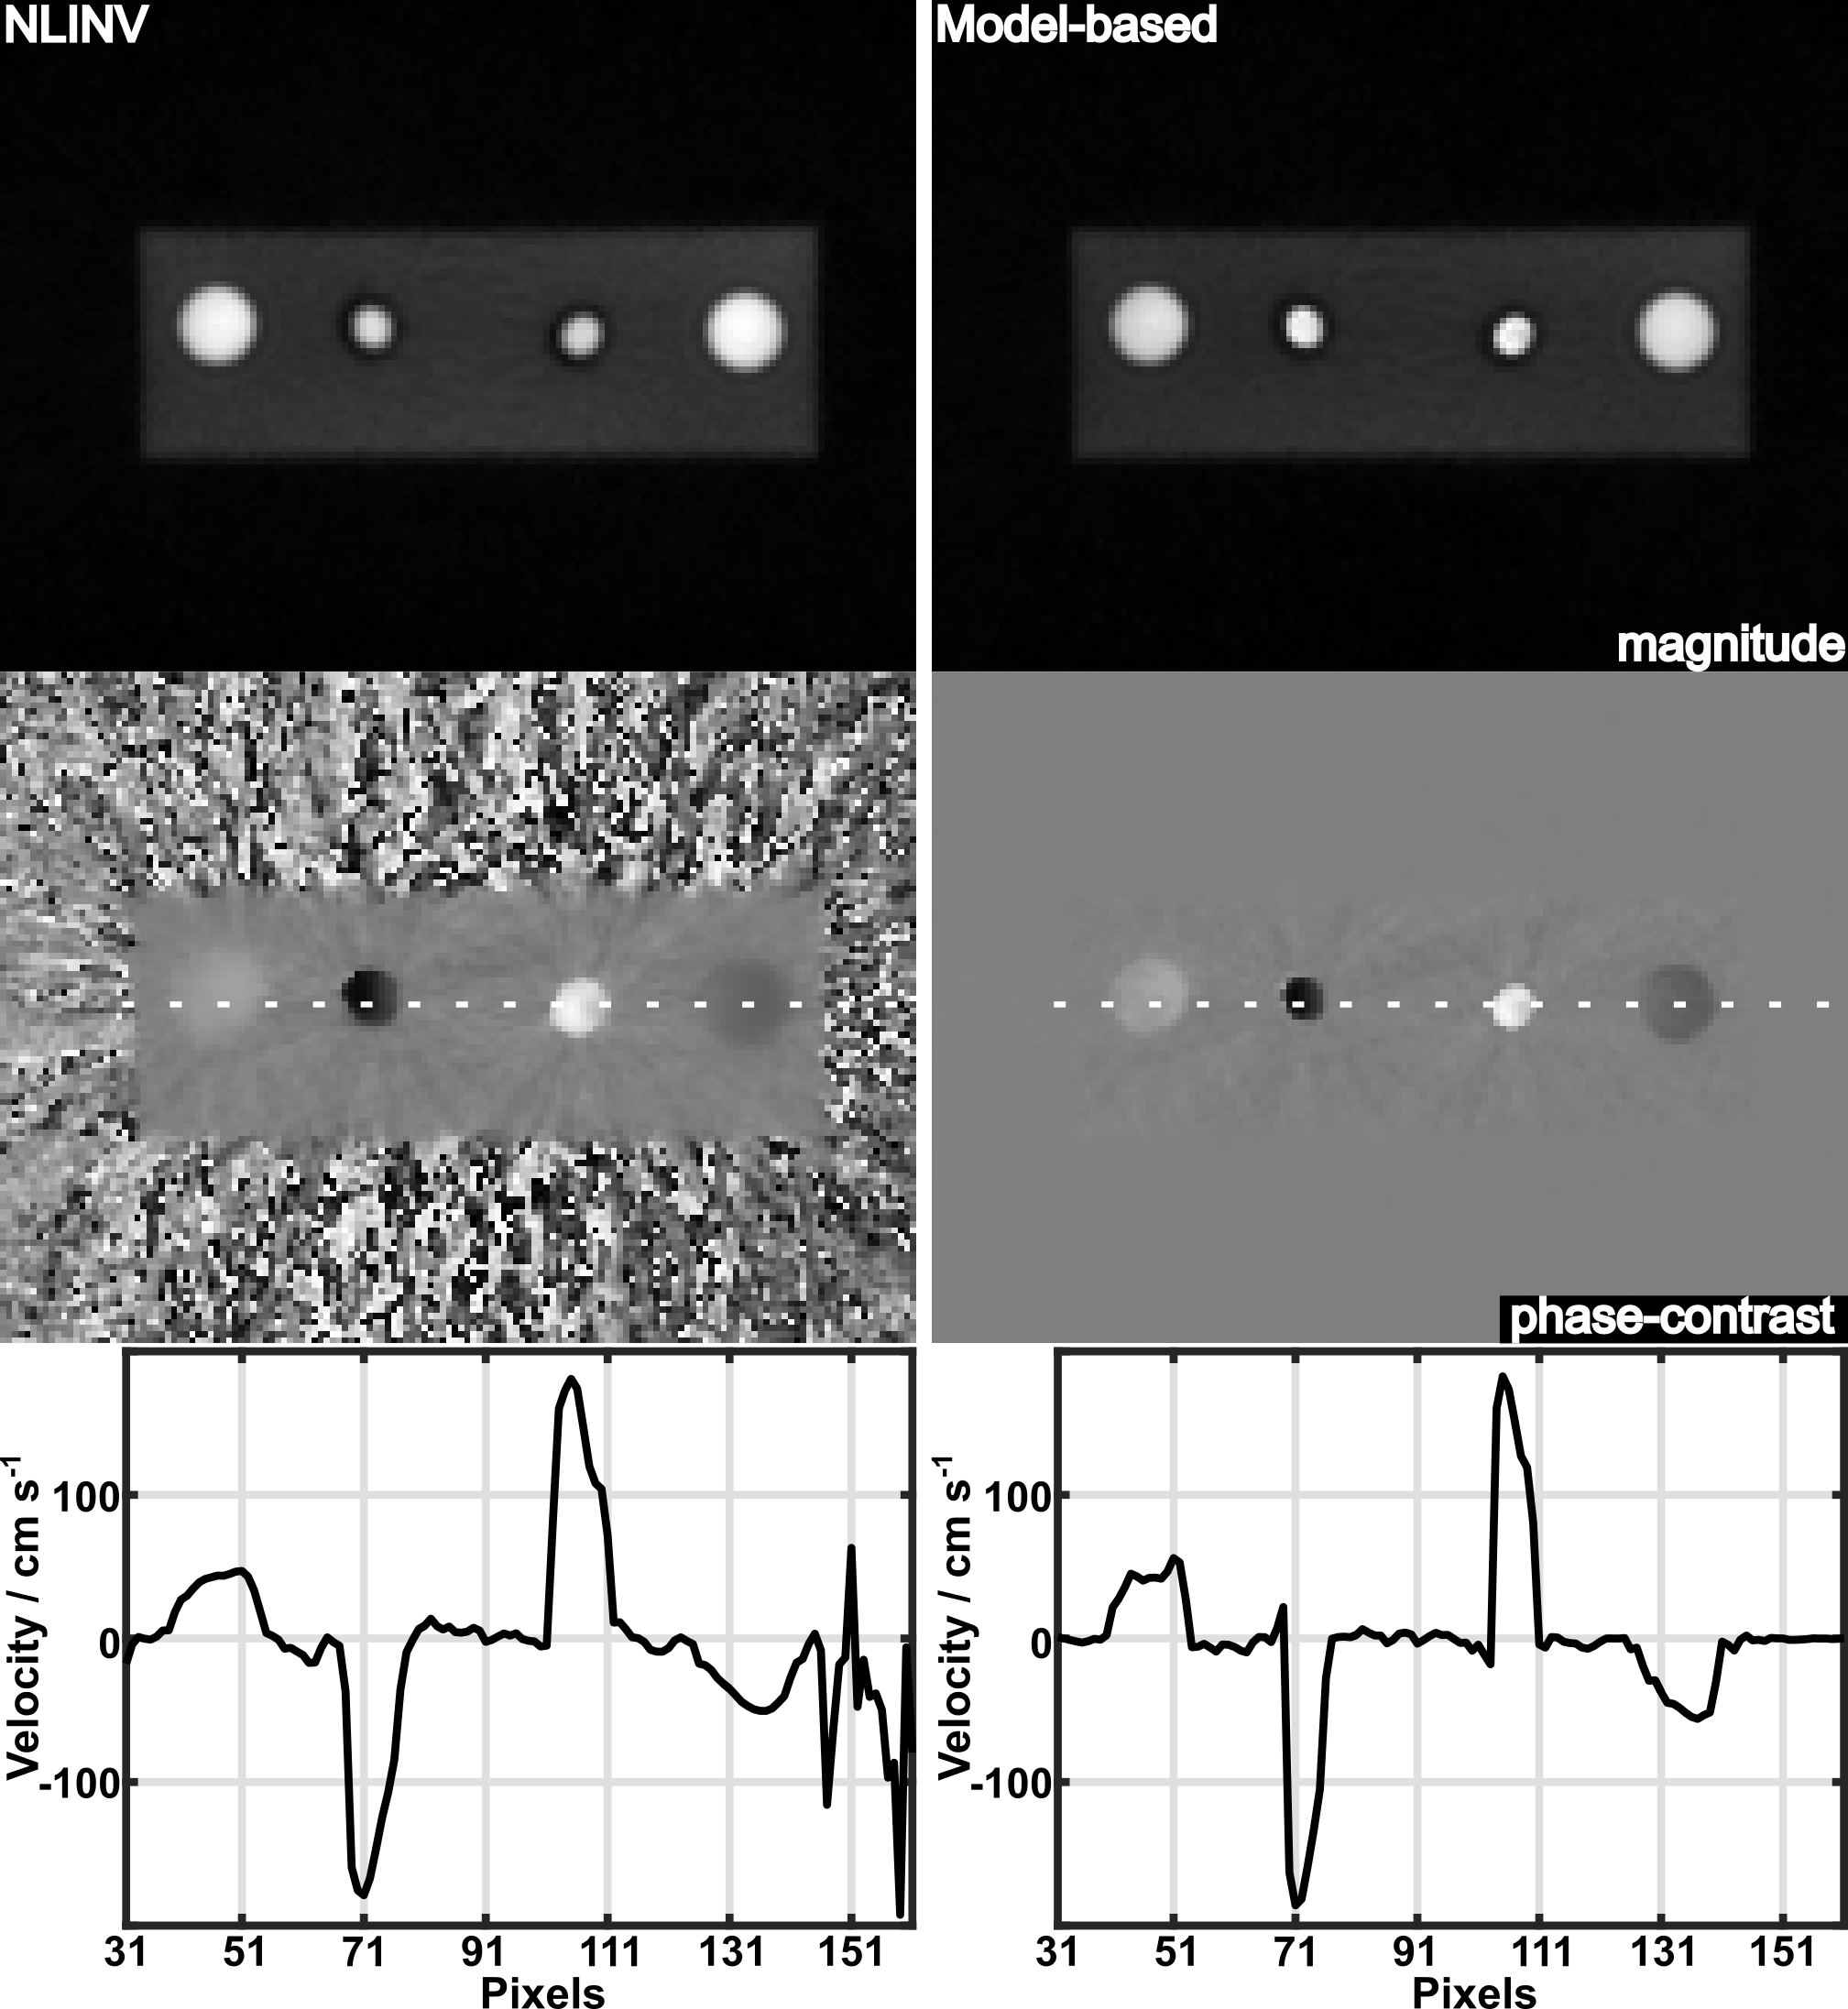
\includegraphics[width=0.8\textwidth]{fig/mir-pc-exp-pha.png}
  \caption{(Left) NLINV and (right) model-based reconstructions of (top) magnitude images and phase-contrast maps as well as (bottom) velocity profiles (along indicated reference lines) for an experimental flow phantom with constant (bidirectional) flow (tubes No.1 to No.4 from left to right, compare \cref{Tab:mir-pc-exp-pha}). The results were obtained for real-time phase-contrast flow MRI at \SI{33.3}{\ms} resolution and $\text{VENC} = \SI{200}{\cm\per\second}$. Residual streaking artifacts in the NLINV phase-contrast map are reduced in the model-based reconstruction which further improves the spatial definition of all tubes (compare \cref{Tab:mir-pc-exp-pha}).} \label{Fig:mir-pc-exp-pha}
\end{figure}

\begin{table}[tb]
  \caption{Quantitative evaluations of an experimental flow phantom}
  \label{Tab:mir-pc-exp-pha}
  \begin{center}
	\begin{threeparttable}
	  \begin{tabular}{ c 
					   c 
					   S[table-format=3] 
					   S[table-format=3] 
					   S[table-format=-3] 
					   S[table-format=-1.1] 
					 }
		\toprule
	    \multirow{3}{*}{{Tube\textsuperscript{1}}} & \multirow{3}{*}{{Method}} & {Magnitude} & {Phase-Contrast} & {Peak} & {Flow} \\
	     & & {Image\textsuperscript{2}} & {Map}               & {Velocity}              & {Volume\textsuperscript{3}} \\
         & & {(\si{\square\mm})}        & {(\si{\square\mm})} & {(\si{\cm\per\second})} & {(\si{\L\per\minute})} \\
	    \midrule
	    \multirow{2}{*}{No.1} & NLINV       & 255 & 360 & 55   & 6.5  \\
                              & Model-based & 239 & 243 & 63   & 6.8  \\
	    \hline
	    \multirow{2}{*}{No.2} & NLINV       & 76  & 131 & -189 & -7.3 \\
		                      & Model-based & 71  & 75  & -180 & -6.5 \\  
	    \hline
	    \multirow{2}{*}{No.3} & NLINV       & 78  & 139 & 181  & 6.9  \\
	                          & Model-based & 73  & 75  & 185  & 6.9  \\  
	    \hline
	    \multirow{2}{*}{No.4} & NLINV       & 255 & 302 & -52  & -7.0 \\
	                          & Model-based & 235 & 233 & -58  & -6.8 \\
	    \bottomrule
	  \end{tabular}
  
	  \begin{tablenotes}
	    \small
	    \item[1] Tube No.1 to No.4 are shown in \cref{Fig:mir-pc-exp-pha}.
	    \item[2] Estimated tube sizes from high-resolution MRI are about \SI{250}{\square\mm} (No.1, No.4) and \SI{70}{\square\mm} (No.2, No.3).
	    \item[3] The flow volume as determined by a flow meter was \SI{6.3}{\L\per\minute}.
	  \end{tablenotes}
    \end{threeparttable}
  \end{center}
\end{table}

\clearpage

\subsection{Human Studies}
Qualitative comparisons of NLINV and model-based phase-contrast MRI are depicted in \cref{Fig:mir-pc-vol-7s} for a normal subject and in \cref{Fig:mir-pc-pat} for a patient with aortic valve insufficiency and partial stenosis, respectively. In line with results for the experimental flow phantom, the systolic phase-contrast maps obtained by the model-based reconstruction yield a much better spatial definition in regions with non-zero flow (i.e., vessels). Here, this particularly applies to the descending aorta whose phase-difference presentation is in close agreement with the vessel lumen in the magnitude image. In quantitative terms the analysis of peak systolic frames from 10 consecutive heartbeats of the subject shown in \cref{Fig:mir-pc-vol-7s} revealed \SI{445+-16}{\square\mm} (\SI{781+-20}{\square\mm}) for the lumen of the descending (ascending) aorta in model-based phase-contrast maps vs \SI{569+-41}{\square\mm} (\SI{880+-18}{\square\mm}) for NLINV reconstructions.

In addition, the implicit a priori knowledge of zero phase in pixels without flowing spins precludes the iterative optimization process to generate residual streaking artifacts in areas around vessels with maximum systolic flow, i.e. for signals with high temporal and spatial frequencies that are most severely affected by k-space undersampling. Quantitative results for both NLINV and model-based reconstructions are summarized in \cref{Tab:mir-pc-old-dat} for 5 subjects and 2 patients studied previously \cite{2015_PC_Asym} and found to be in general agreement. In comparison to \cite{2015_PC_Asym} all analyses were performed with an extended gradient-delay correction (unpublished results) and evaluated with an updated software package for automatic vessel segmentation (CAIPI Prototype Software). In more detail, while peak velocities obtained by NLINV and model-based reconstruction reveal excellent agreement, stroke volumes (and cardiac output) which rely on integrated velocities over space and time are slightly lower for model-based reconstructions. This observation reflects the sharper (i.e., smaller) definition of the vessel lumen and must not be considered a flaw but an advantage.

The spatiotemporal improvement achievable by model-based phase-contrast flow MRI may be invested into even faster acquisitions. As already suggested by the numerical simulations presented in \cref{Fig:mir-pc-sim-pha} and \cref{Tab:mir-pc-sim-pha}, \cref{Fig:mir-pc-vol-7s-5s} advances NLINV and model-based phase-contrast flow acquisitions from \num{7} spokes per image and \SI{35.7}{\ms} total acquisition time to \num{5} spokes and \SI{25.6}{\ms} resolution. At peak systole the findings of excellent vessel definition with almost no phase noise and residual streakings confirm the expectations from numerical and experimental validations. Together, these findings clearly support the notion that the use of \num{5} spokes represents an extreme but feasible approach to real-time flow MRI at high temporal resolution. This is further confirmed by the quantitative evaluations in \cref{Tab:mir-pc-new-dat} summarizing peak velocities and flow rates for \num{5} additional subjects and acquisitions with \num{7} and \num{5} spokes. Regardless of possible intrasubject variability in repetitive measurements, mean peak velocities and flow volumes (10 heartbeats) in both the ascending and descending aorta differ by less than \SI{4}{\percent} when comparing \SI{35.7}{\ms} acquisitions (\num{7} spokes) with \SI{25.6}{\ms} acquisitions (\num{5} spokes).
\vspace{10mm}

\begin{figure}[h!]
  \centering
  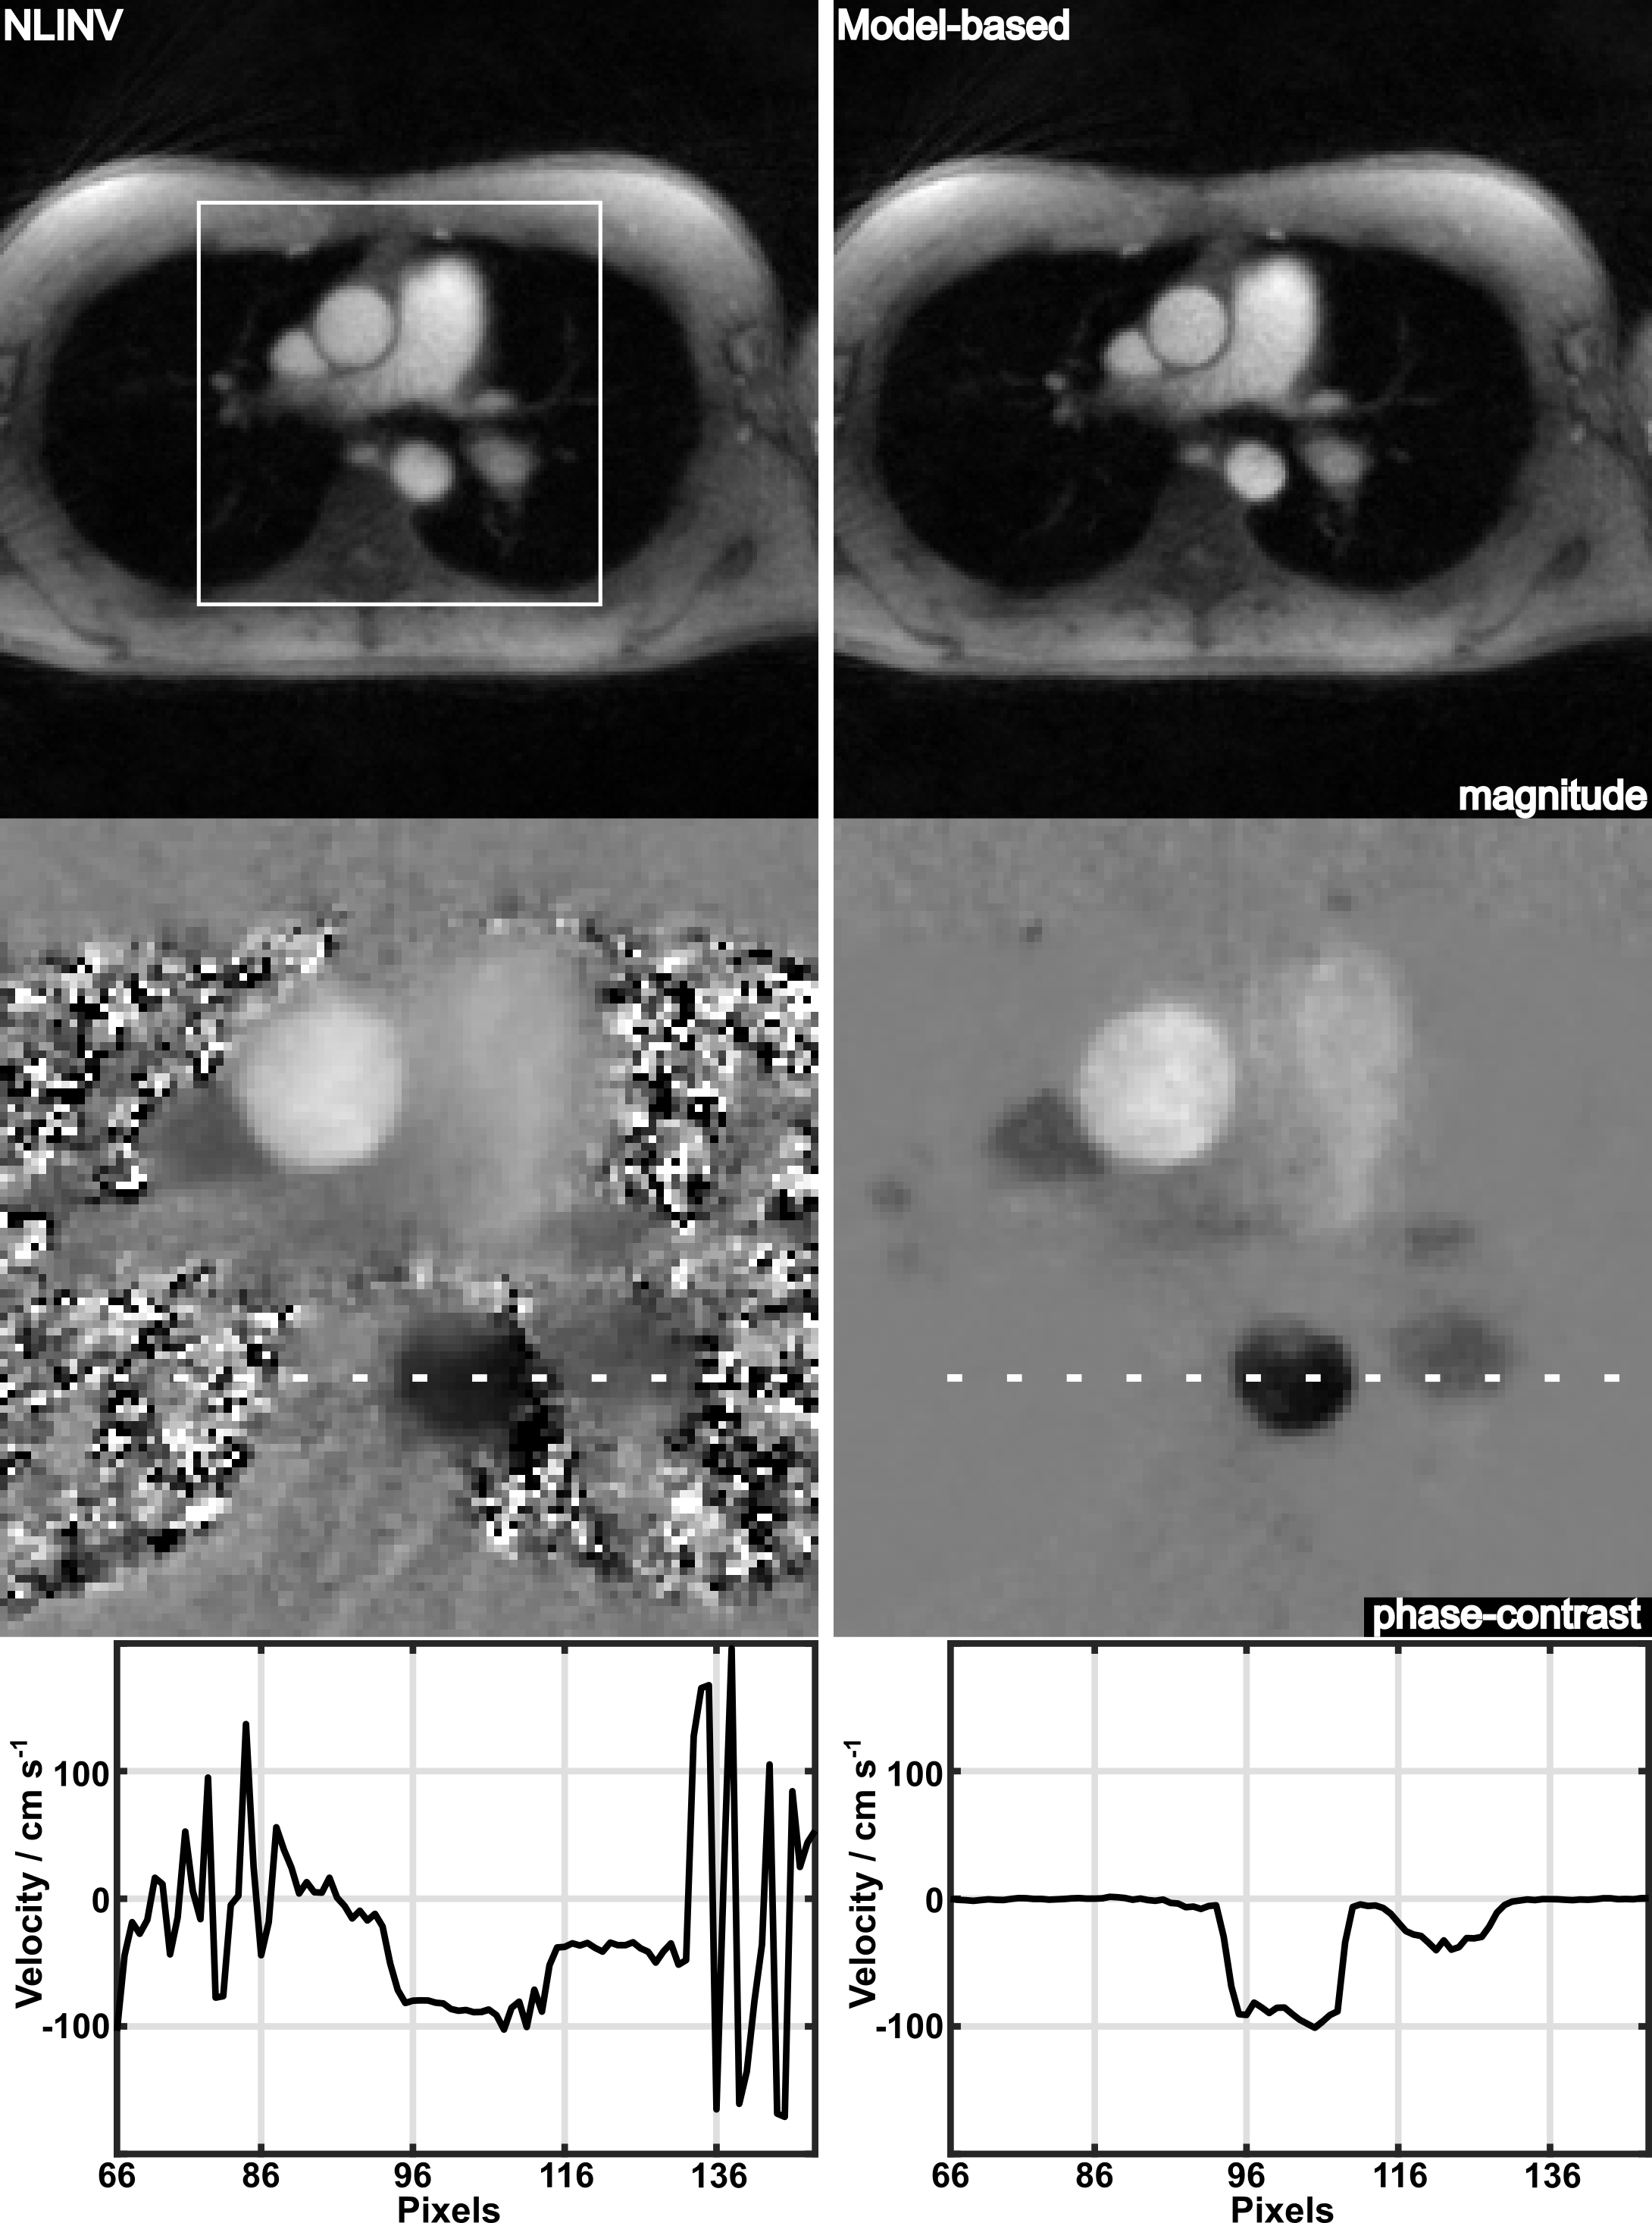
\includegraphics[width=0.8\textwidth]{fig/mir-pc-vol-7s.png}
  \caption{(Left) NLINV and (right) model-based reconstructions of (top) systolic magnitude images and phase-contrast maps (magnified views) as well as (bottom) velocity profiles (along indicated reference lines) for real-time phase-contrast MRI of aortic blood flow in a healthy volunteer at \SI{35.7}{\ms} resolution and $\text{VENC} = \SI{200}{\cm\per\second}$.} \label{Fig:mir-pc-vol-7s}
\end{figure}

\begin{figure}[tb]
  \centering
  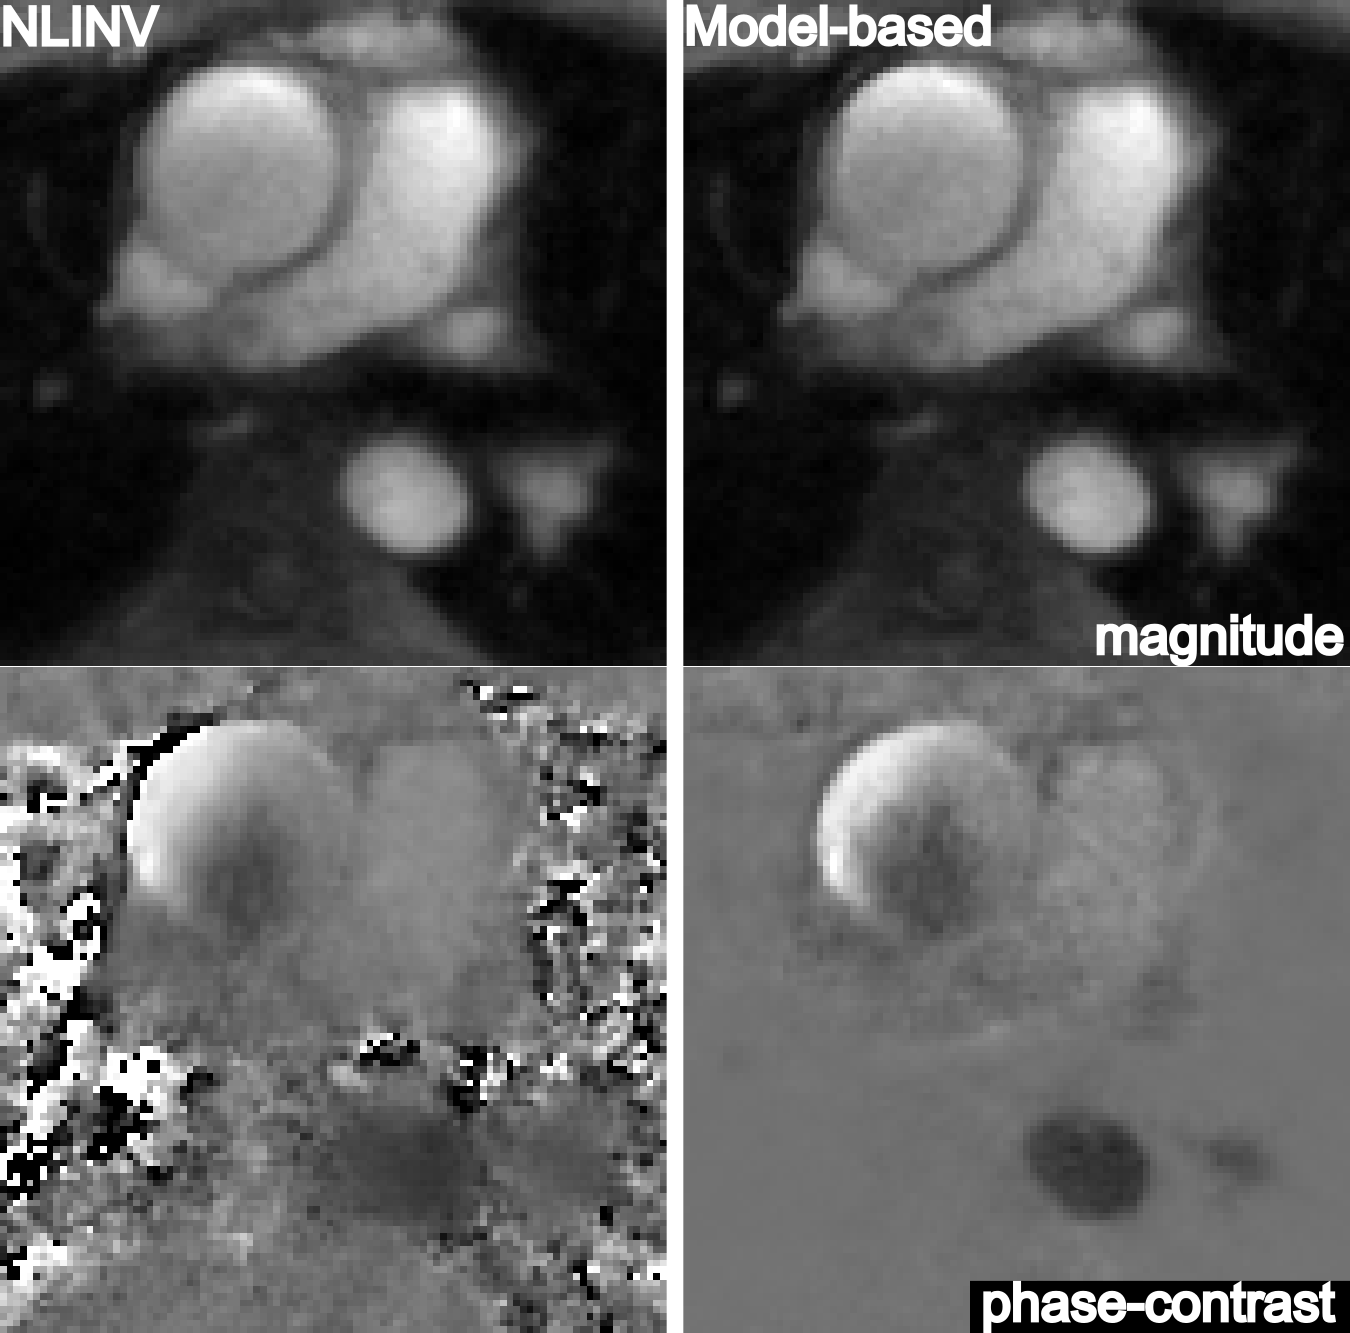
\includegraphics[width=0.80\textwidth]{fig/mir-pc-pat.png}
  \caption{(Left) NLINV and (right) model-based reconstructions of systolic magnitude images and phase-contrast maps (magnified views) for real-time phase-contrast MRI of a patient with aortic valve insufficiency and partial stenosis at \SI{35.7}{\ms} resolution and $\text{VENC} = \SI{400}{\cm\per\second}$.} \label{Fig:mir-pc-pat}
\end{figure}

\begin{table}[tb]
  \caption{Quantitative flow evaluations of the ascending aorta of healthy volunteers and patients with valve insufficiency (data from Ref.~\cite{2015_PC_Asym}). The results represent mean values $\pm$ standard deviation for \num{10} consecutive heartbeats at \SI{35.7}{\ms} resolution.}
  \label{Tab:mir-pc-old-dat}
  \begin{center}
	\begin{tabular}{ c 
					 c 
					 S[table-format=3(2)]
					 S[table-format=3(1)] 
					 S[table-format=1.1(2)] 
					 S[table-format=2(1)] 
				   }
	  \toprule
	  \multirow{3}{*}{Subject}   & \multirow{3}{*}{Method} & {Peak}                  & {Flow per}        & {Flow}                 & {Regurgitation}   \\
	                             &                         & {Velocity}              & {Heartbeat}       & {Volume}               & {Fraction}        \\
	                             &                         & {(\si{\cm\per\second})} & {(\si{\milli\L})} & {(\si{\L\per\minute})} & {(\si{\percent})} \\
	  \midrule
	  \multirow{2}{*}{No.1} & {NLINV}       & 120 \pm 3   & 99 \pm 4  & 5.7 \pm 0.4 & 2 \pm 1 \\
	                        & {Model-based} & 121 \pm 4   & 91 \pm 5  & 5.2 \pm 0.4 & 1 \pm 1 \\
	  \hline
	  \multirow{2}{*}{No.2} & {NLINV}       & 114 \pm 8   & 124 \pm 6 & 6.9 \pm 0.3 & 1 \pm 1 \\
	                        & {Model-based} & 114 \pm 7   & 112 \pm 5 & 6.3 \pm 0.2 & 1 \pm 1 \\
	  \hline
	  \multirow{2}{*}{No.3} & {NLINV}       & 69 \pm 3    & 61 \pm 3  & 4.0 \pm 0.2 & 2 \pm 1 \\
	                        & {Model-based} & 76 \pm 4    & 62 \pm 2  & 4.1 \pm 0.2 & 1 \pm 1 \\
	  \hline
	  \multirow{2}{*}{No.4} & {NLINV}       & 112 \pm 5   & 131 \pm 4 & 8.1 \pm 0.3 & 2 \pm 1 \\
	                        & {Model-based} & 111 \pm 4   & 123 \pm 4 & 7.6 \pm 0.3 & 2 \pm 1 \\  
	  \hline
	  \multirow{2}{*}{No.5} & {NLINV}       & 100 \pm 5   & 107 \pm 3 & 6.2 \pm 0.1 & 3 \pm 1 \\
	                        & {Model-based} & 109 \pm 5   & 97 \pm 3  & 5.6 \pm 0.1 & 4 \pm 1 \\
	  \hline
	  \multirow{2}{*}{Pat.1} & {NLINV}       & 264 \pm 14 & 56 \pm 6  & 3.0 \pm 0.3 & 55 \pm 3 \\
	                         & {Model-based} & 216 \pm 11 & 51 \pm 4  & 2.8 \pm 0.2 & 57 \pm 2 \\
	  \hline
	  \multirow{2}{*}{Pat.2} & {NLINV}       & 222 \pm 12 & 82 \pm 5  & 5.3 \pm 0.3 & 18 \pm 2 \\
	                         & {Model-based} & 219 \pm 6  & 71 \pm 6  & 4.6 \pm 0.4 & 23 \pm 3 \\
	  \bottomrule
	\end{tabular}
  \end{center}
\end{table}


\begin{figure}[tb]
  \centering
  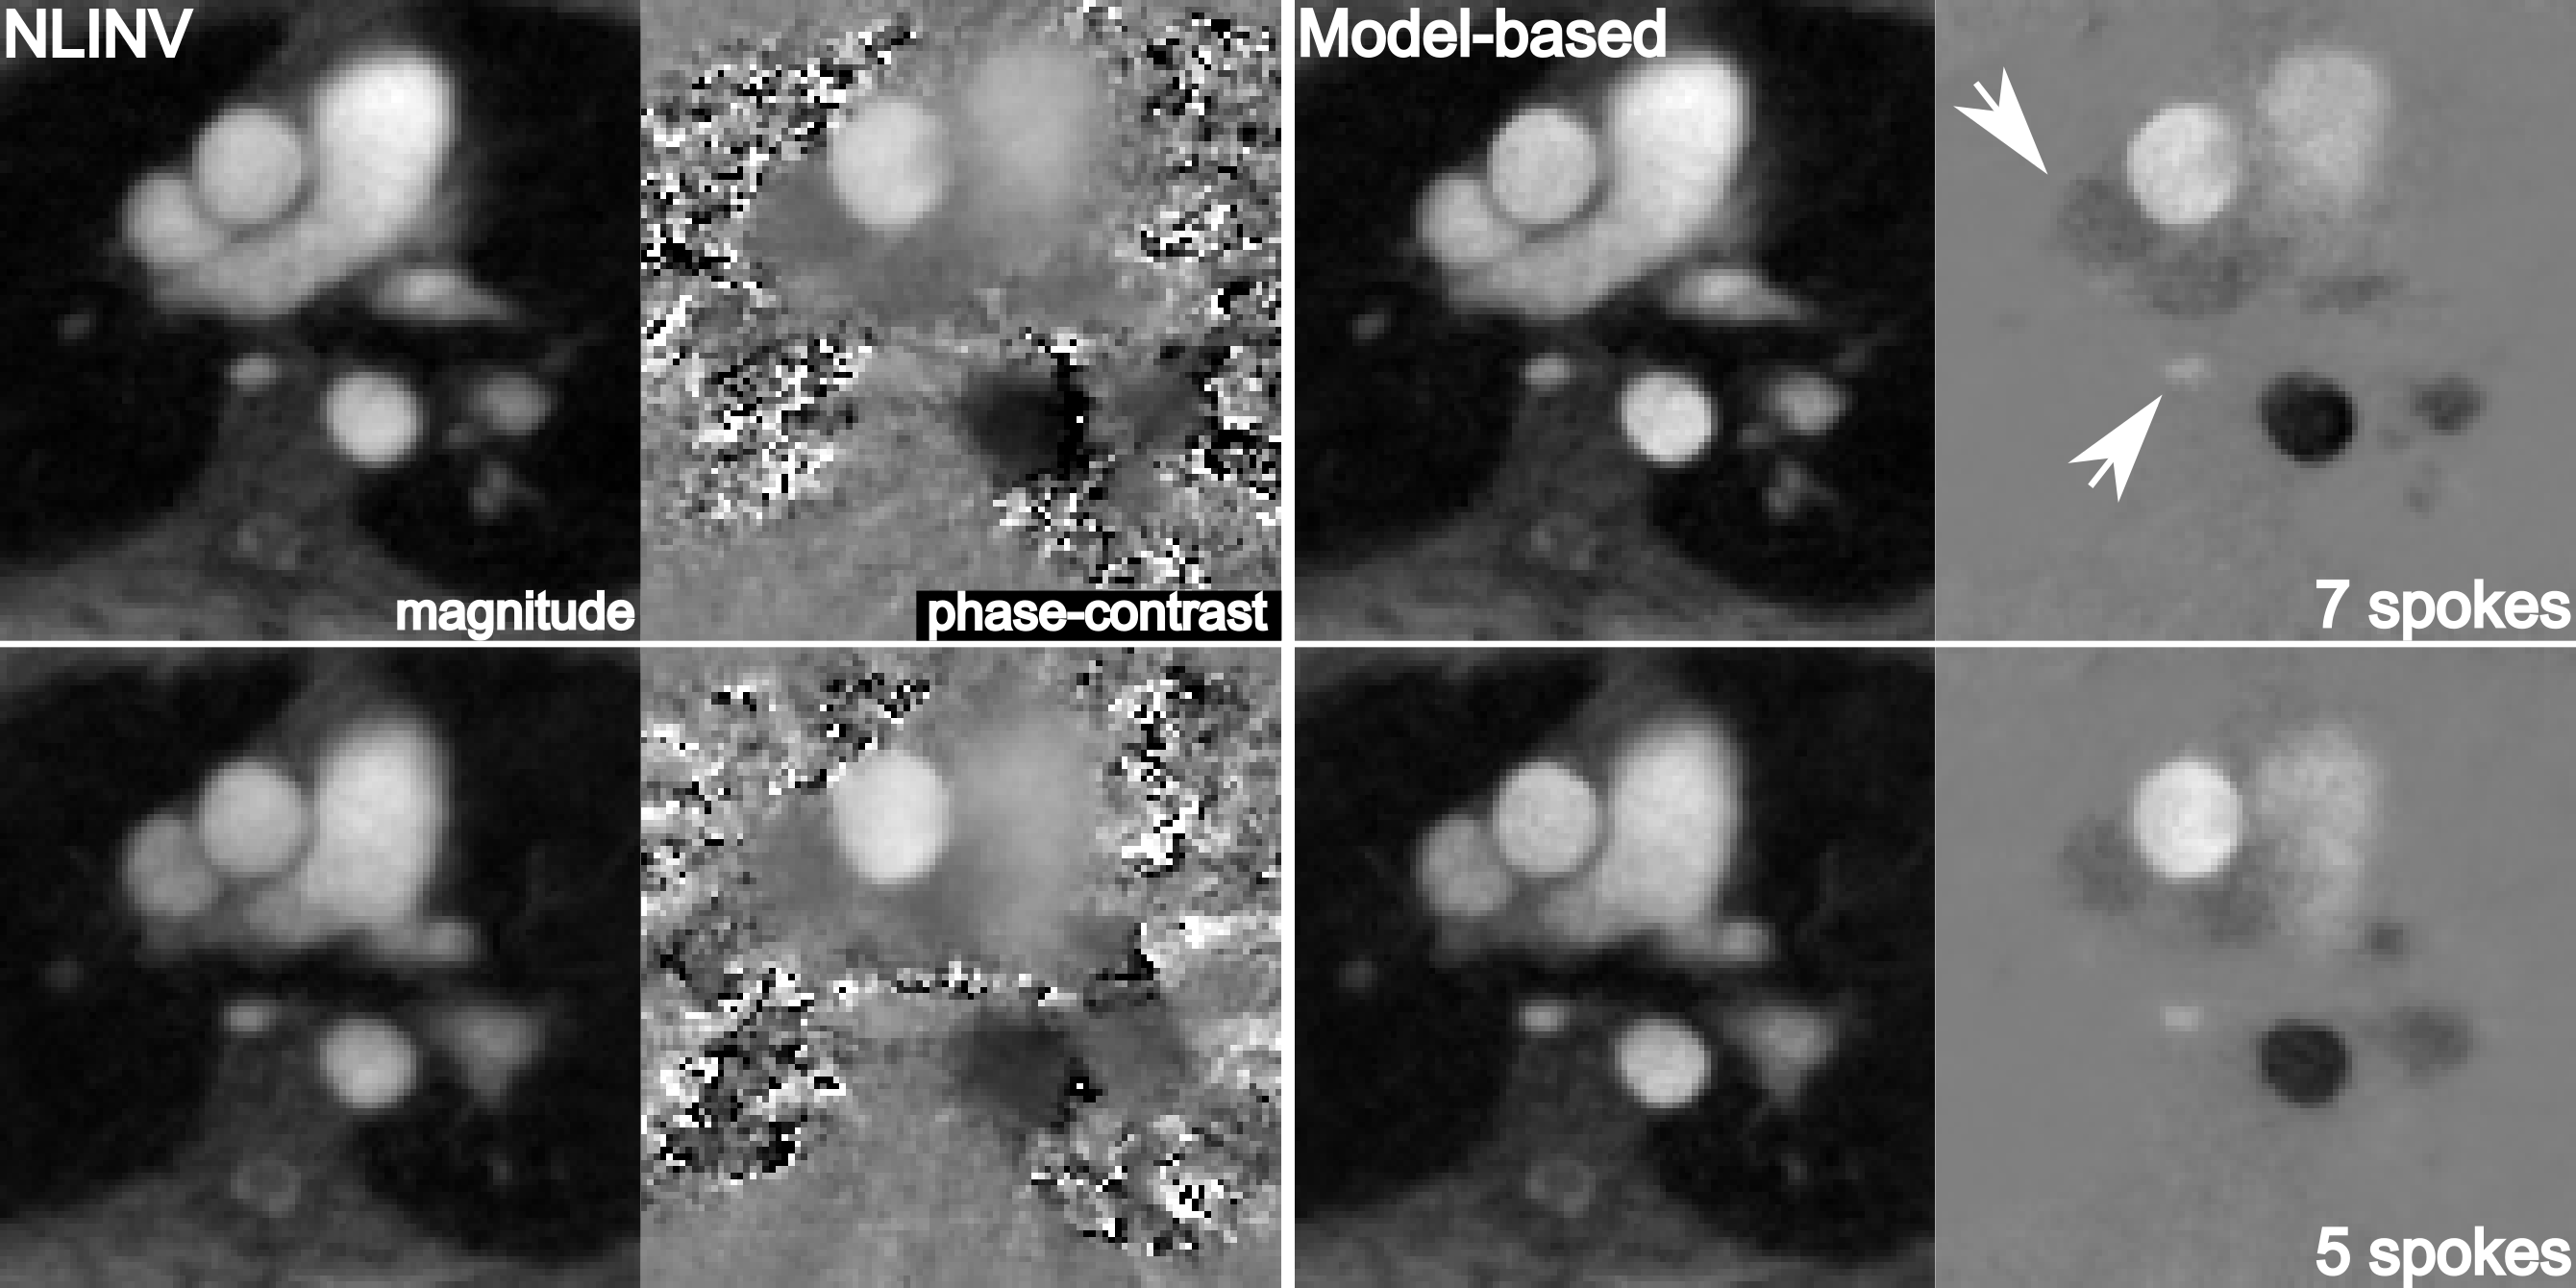
\includegraphics[width=\textwidth]{fig/mir-pc-vol-7s-5s.png}
  \caption{(Left) NLINV and (right) model-based reconstructions of systolic magnitude images and phase-contrast maps (magnified views) for real-time phase-contrast MRI of aortic blood flow (VENC = 200 cm s\textsuperscript{-1}) in a healthy volunteer using (top) 7 spokes per frame at 35.7 ms resolution and (bottom) 5 spokes at 25.6 ms resolution. Note the improved delineation of the superior vena cava (upper arrow) and the small azygos vein (lower arrow) in model-based phase-contrast maps.} \label{Fig:mir-pc-vol-7s-5s}
\end{figure}

\begin{table}[tb]
  \caption{Quantitative flow evaluations of model-based reconstructions in the ascending and descending aorta of healthy volunteers. The results represent mean values $\pm$ standard deviation for 10 consecutive heartbeats at \SI{35.7}{\ms} and \SI{25.6}{\ms} resolution, respectively. The bottom row presents percent differences of mean values for acquisitions at \SI{35.7}{\ms} and \SI{25.6}{\ms} resolution.}
  \label{Tab:mir-pc-new-dat}
  \begin{center}
	\begin{tabular}{ c 
					 c 
					 S[table-format=-3(2)] 
					 S[table-format=-3(1)] 
					 S[table-format=-3(1)] 
					 S[table-format=2(2)] }
	                           &          & \multicolumn{2}{c}{\textbf{Ascending Aorta}} & \multicolumn{2}{c}{\textbf{Descending Aorta}} \\
	  \toprule
	  \multirow{3}{*}{Subject} & {Spokes} & {Peak}                  & {Flow per}         & {Peak}                  & {Flow per}          \\
	                           & {per}    & {Velocity}              & {Heartbeat}        & {Velocity}              & {Heartbeat}         \\
	                           & {Image}  & {(\si{\cm\per\second})} & {(\si{\milli\L})}  & {(\si{\cm\per\second})} & {(\si{\milli\L})}   \\
	  \midrule
	  \multirow{2}{*}{No.6}    & 7        & 88 \pm 4  & 96 \pm 9  & 99 \pm 5  & 58 \pm 5 \\
	                           & 5        & 89 \pm 4  & 100 \pm 4 & 103 \pm 5 & 70 \pm 3 \\
	  \hline
	  \multirow{2}{*}{No.7}    & 7        & 127 \pm 6 & 107 \pm 6 & 128 \pm 5 & 81 \pm 4 \\
	                           & 5        & 116 \pm 6 & 94 \pm 5  & 120 \pm 6 & 68 \pm 4 \\
	  \hline
	  \multirow{2}{*}{No.8}    & 7        & 83 \pm 7  & 77 \pm 7  & 104 \pm 4 & 52 \pm 4 \\
	                           & 5        & 84 \pm 10 & 76 \pm 7  & 104 \pm 6 & 55 \pm 4 \\
	  \hline
	  \multirow{2}{*}{No.9}    & 7        & 114 \pm 3 & 106 \pm 4 & 119 \pm 3 & 60 \pm 3 \\
	                           & 5        & 115 \pm 2 & 103 \pm 5 & 115 \pm 3 & 60 \pm 4 \\
	  \hline
	  \multirow{2}{*}{No.10}   & 7        & 96 \pm 4  & 81 \pm 3  & 100 \pm 5 & 54 \pm 3 \\
	                           & 5        & 96 \pm 3  & 75 \pm 4  & 100 \pm 3 & 54 \pm 3 \\
	  \hline
	  {Diff. (\si{\percent})}  & 7 vs 5   & -1 \pm 4  & -4 \pm 6  & -1 \pm 4  & 2 \pm 13 \\
	  \bottomrule
    \end{tabular}
  \end{center}
\end{table}

\clearpage

\section{Discussion}
This work demonstrates the successful development of a model-based reconstruction technique for real-time phase-contrast flow MRI and its application to the assessment of cardiovascular blood flow. When compared to a previous flow MRI method based on NLINV reconstructions of two independent flow-compensated and flow-encoded images \cite{2015_PC_Asym}, the flow results are quantitatively accurate, while the images and maps present with improved spatial acuity and reduced residual streaking artifacts. Most importantly, the desired phase-difference maps reveal much reduced phase noise when compared to phase-difference maps of two complex images with arbitrary phases, in particular in areas of low or no MRI signal. As a consequence, the proposed method offers much better access to small vessels such as for example the azygos vein (see \cref{Fig:mir-pc-vol-7s-5s}). On the other hand, the improved image quality and vessel definition of the model-based phase-contrast method allows for the use of only \num{5} spokes per image which pushes flow MRI to a temporal resolution of \SI{25.6}{\ms} or a rate of \num{39} phase-contrast maps per second. Similar degrees of radial undersampling (i.e., \num{5} spokes per image) have already successfully been applied for real-time MRI studies of high-speed tongue movements in elite horn players \cite{2015_horn_QIM} and experimentally been demonstrated to provide excellent temporal fidelity for a rapid motion phantom \cite{2014_Temp_Fidelity} when eliminating any temporal filter as done here for the velocity-encoded phase-contrast maps.

At this time, the most relevant limitation of the proposed method is the need for a time-consuming offline calculation. Although conventional NLINV reconstructions are available online for immediate control \cite{2015_PC_Asym}, the nonlinear inverse problem posed by the phase-contrast flow MRI signal model requires new efforts for parallelization, GPU programming and implementation on the existing bypass server to the host computer of our MRI system. Nevertheless, such work will be mandatory to provide an online version for extended clinical trials. Another future option might be a comparative investigation of other model-based flow MRI methods and their applicability to highly undersampled MRI data. However, such studies are outside the scope of the present work, which offers multiple validations of the proposed model-based reconstruction for real-time flow MRI comprising numerical simulations, an experimental phantom, normal subjects and patients with previous ECG-synchronized flow MRI data \cite{2015_PC_Asym}.

An advantageous extension of the current model-based reconstruction may arise from the fact that the method is applicable to arbitrary trajectories in k-space, and in particular, to different spatial encodings (i.e., sets of spokes) for the flow-encoded and flow-compensated dataset. So far, most if not all phase-contrast MRI acquisition techniques including the one used here, employ the same lines in k-space when comparing phase differences between flow-compensated and flow-encoded acquisitions. However, the use of complementary sets of radial spokes, e.g.~in two sequential acquisitions, offers at least two advantages: First, it promises to increase the spatial resolution (and computational robustness) of respective model-based reconstructions. This can be seen from the adjoint operator in \cref{Equ:adj}, where the summation of indices $l$ for d$\rho$ and d$z$ accumulates all available spatial samples. Secondly, the use of different encodings in k-space, eventually in combination with two similar but sign-inverted bipolar flow-encoding gradients, will allow for a sliding-window approach where model-based reconstructions are shifted by just one dataset (here \num{7} or \num{5} spokes) rather than two datasets and thereby improve the effective temporal resolution by a factor of two (here to about \num{18} or \SI{13}{\ms}). Along the same idea, it seems reasonable to extend the model-based concept from one-dimensional (i.e., through-plane) flow to the analysis of phase-contrast MRI studies with three-dimensional velocity encodings.

In conclusion, the present work introduces a novel model-based reconstruction technique for velocity-encoded phase-contrast flow MRI which simultaneously estimates a proton density map, a phase-contrast map and a set of coil sensitivity profiles from each pair of flow-encoded and flow-compensated datasets. The solution to the resulting nonlinear inverse problem is accomplished with the use of IRGNM. When based on highly undersampled radial FLASH acquisitions, real-time applications benefit from reduced noise and improved spatial accuracy of the computed phase-contrast maps which therefore allow for a temporal resolution of \SI{25.6}{\ms} per flow map.



\chapter{Multi-Echo Radial FLASH} \label{Chp:multi-echo}
\chaptermark{Multi-Echo Radial FLASH}

%The conventional \textit{multi-echo} radial FLASH utilizes bipolar readout gradients with the same amplitude and duration to sample echoes in a fly-back-and-forth manner, which, however, is not efficient enough in the respects of k-space coverage and temporal resolution. Therefore, the multi-echo multi-spoke radial FLASH sequence, which acquires multiple echoes with different spatial encodings per RF excitation, is proposed for the purposes of faster k-space sampling and better temporal resolution. In addition, a nonlinear inverse reconstruction that jointly estimates all echo images and coil sensitivity maps is investigated.
%In this chapter, two types of multi-echo radial FLASH sequences with preliminary results including phantom, human brain and cardiac studies are presented. 

\section{Introduction}
Multi-gradient-echo sequences contain two intrinsic properties. First, they acquire multiple echoes after one RF excitation, which substantially shortens imaging time when echoes are differently encoded. Note that one TR interval in these sequences is also named one echo-train. Second, they elongate TE and TR, resulting in \acs{T2s}-weighted image contrast and off-resonance phase modulations among echoes. $T_2^*$ signal decay is a direct indication of the blood-oxygen-level dependent (\acs{BOLD}) contrast primarily used in functional MRI (\acs{fMRI}), discovered by Ogawa et al.~in 1990 \cite{1990_fMRI}. Nowadays, the most frequently used sequence for fMRI is echo-planar imaging (\acs{EPI}) \cite{1998_EPI} proposed by Peter Mansfield, who was awarded the 2003 Nobel Prize in Physiology or Medicine, shared with Paul Lauterbur. On the other hand, off-resonance phase modulations represent tissue susceptibility differences. Their quantification has been the key to susceptibility-weighted imaging \cite{2015_SWI_QSM} and water-fat separation \cite{2004_IDEAL}.

Multi-gradient-echo is usually combined with Cartesian sampling, which, however, results in images with severe spatial distortion due to off-resonance phase modulation. Although several methods have been proposed for off-resonance estimation and correction (e.g.~see \cite{1999_off-reson_cor,1999_EPI_off-reson_MEGE,2004_fim_est_spiral,2005_Toeplitz_fim_cor,2008_fim_est,2008_r2s_fm_fMRI,2009_fim_t2s_me_TMI,2012_ORACLE,2014_fim_est}), research endeavors have also been made toward combining multi-echo gradient-echo sequences and radial sampling. Silva et al.~\cite{1998_rEPI} proposed radial EPI that acquires all designated spokes with only one RF excitation, and revealed via a water-oil phantom that off-resonance phase modulation in rEPI results in blurring and radial streaks but no spatial distortion. Rasche et al.~\cite{1999_prMGE} developed radial multi-gradient-echo MRI using about \num{100} spokes per image and maximally \num{4} echoes (corresponding to about \SI{150}{\ms} temporal resolution) for various in-vivo studies, i.e., swallowing, joint motion, and cardiac fluoroscopy. Larson et al.~\cite{2001_SPIDER} achieved a temporal resolution of \SI{45}{\ms} with an echo-train length (\acs{ETL}) of \num{3} and a factor of 2 view-sharing scheme for real-time cardiac imaging via steady-state projection imaging with dynamic echo-train readout (SPIDER). Here, one echo-train consists of one partial first echo, one full second echo, and one partial third echo. Theilmann et al.~\cite{2004_vo_rFSE,2005_rGRASE} studied four view-ordering schemes in radial fast spin-echo imaging and subsequently developed a radial gradient and spin-echo (GRASE) technique. On the other hand, rEPI with stack-of-stars for 3D imaging was proposed by Bhat et al.~\cite{2011_MRA_rEPI} for contrast-enhanced whole-heart coronary angiography, and true 3D radial multi-echo sequences have also been proposed (e.g.~see \cite{2005_3D_rMHE,2010_3D_rME,2013_MRA_rME}). Furthermore, radial multi-echo sequences was applied to quantitative $T_2^*$ mapping by Winkelmann et al.~\cite{2006_R2s_rMGE}. Note that all these imaging techniques used either gridding \& FFT or parallel imaging as linear inversion for image reconstruction.

The conventional multi-echo radial FLASH utilizes bipolar readout gradients with the same amplitude to sample echoes in a fly-back-and-forth manner, which, however, is not efficient enough with respect to k-space coverage and temporal resolution. Therefore, this thesis developed a multi-echo multi-spoke (\acs{MEMS}) radial FLASH sequence, which acquires multiple echoes with different spatial encodings per RF excitation and connects two successive echoes with blip gradients. For image reconstructions of multi-echo radial FLASH data, a multi-echo NLINV which jointly estimates all echo images and one set of coil sensitivity maps is proposed and compared with the standard NLINV. Moreover, a simple off-resonance estimation and correction method based on the pixel-wise fitting of reconstructed echo images and the conjugate phase reconstruction is implemented to alleviate off-resonance effects. Preliminary results on the human brain and heart demonstrate that the proposed sequence can probably be applied to real-time MRI with improved temporal and spatial resolutions and lead to quantitative mapping of \acs{T2s} relaxation times and off-resonance frequencies in real time.



\section{Theory} 

\begin{figure}[p]
  \centering
  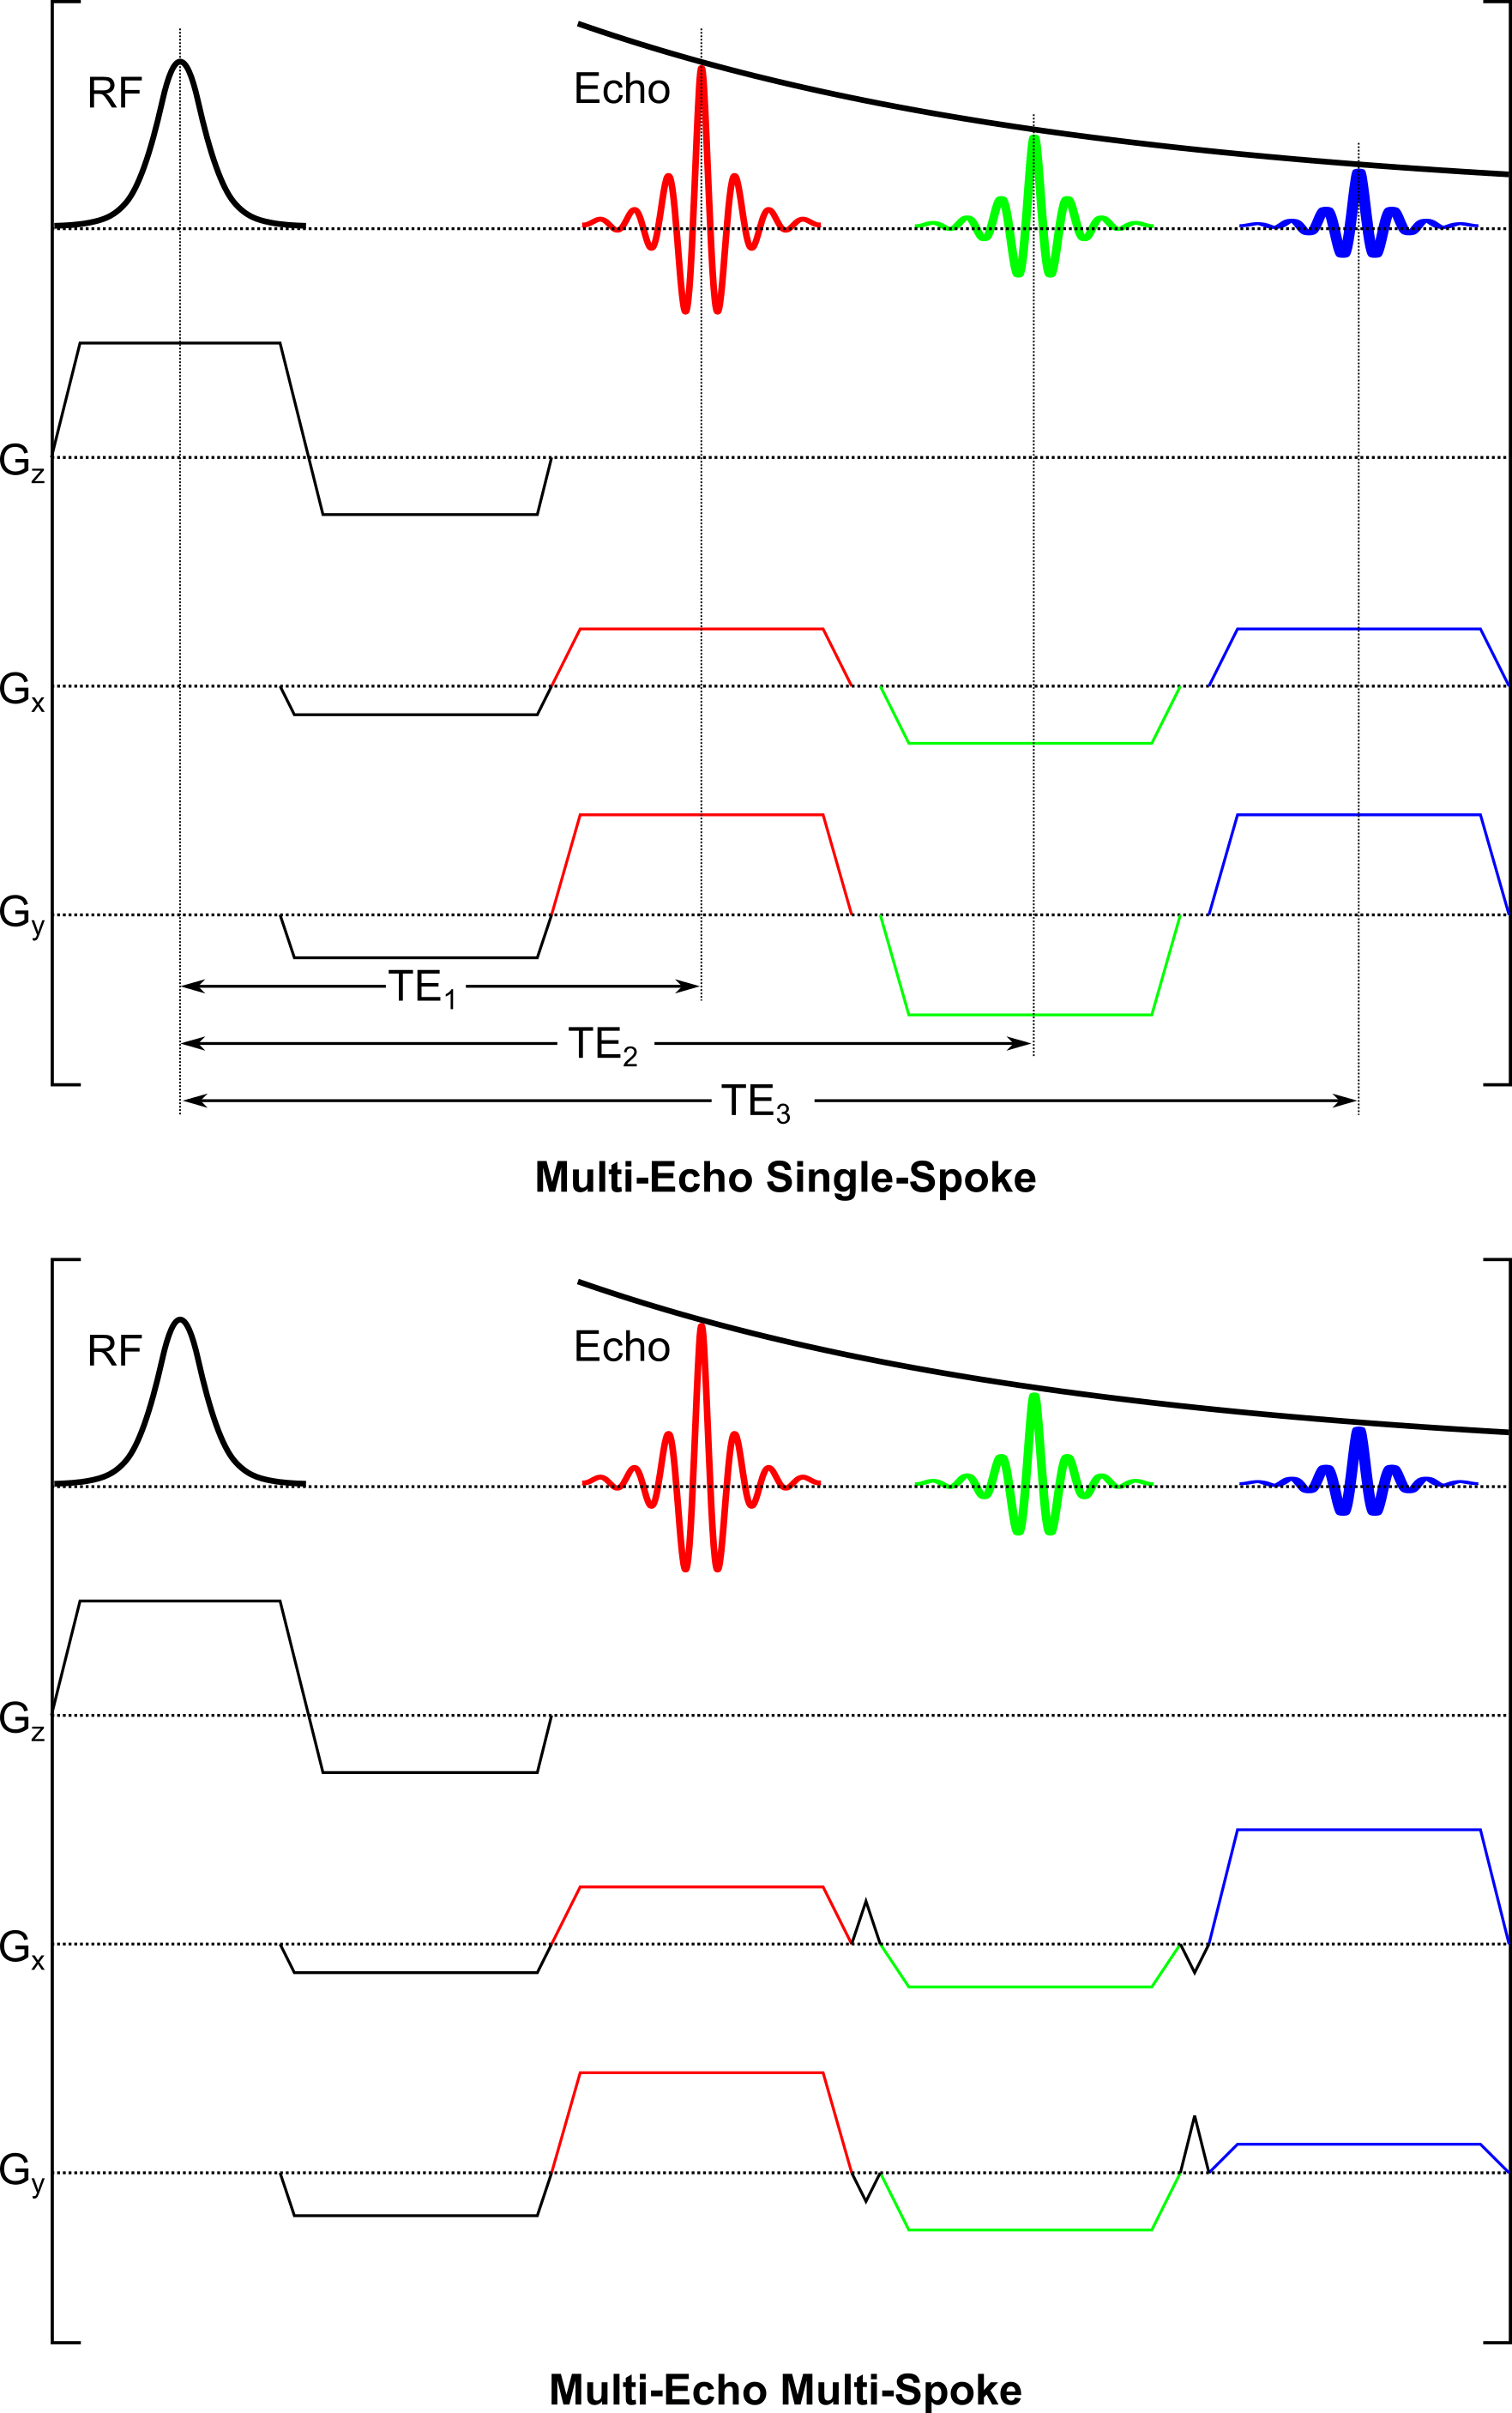
\includegraphics[width=0.80\textwidth]{fig/multi-echo-seq.png}
  \caption{Multi-echo radial FLASH sequences. (Top) Multi-echo single-spoke (\acs{MESS}), where multiple echoes are sampled on one single spoke via bipolar readout gradients with the same magnitude and duration but altered polarity. (Bottom) Multi-echo multi-spoke (\acs{MEMS}), where multiple echoes per RF excitation are sampled on spokes with rotated spatial orientations and concatenated by blip gradients.} \label{Fig:multi-echo-seq}
\end{figure}
\subsection{Multi-Echo Radial FLASH Sequences} \label{Sec:me-theory-seq}
In principle, multi-echo radial FLASH sequences can be divided into two categories depending on the k-space coverage of one echo-train. If only one spoke is sampled back-and-forth via bipolar readout gradients with the same magnitude and duration but altered polarity, this type of sequence is named \textbf{multi-echo single-spoke} (\acs{MESS}), as shown in the top of \cref{Fig:multi-echo-seq}. All echoes within one echo-train have identical spokes but are weighted with $T_2^*$ and off-resonance according to their respective echo times, and one image can be formed by the spokes acquired at the same echo. As a result, MESS renders a total of $L$ echo images with $L$ being the number of echoes per frame measurement. Here, $L$ can be any integer, usually between \num{1} and \num{32}. MESS has been applied to real-time MRI applications \cite{2012_rtmri_app}, i.e., water-fat separation and myocardial $T_2^*$ mapping. On the contrary, if spokes with different spatial orientations are sampled in one echo-train, this type of sequence is named \textbf{multi-echo multi-spoke} (\acs{MEMS}), as shown in the bottom of \cref{Fig:multi-echo-seq}. When compared to MESS, MEMS can speed up the acquisition by a factor of $L$ if both of them sample the same total number of spokes per frame. Moreover, MEMS is more flexible in image formation. An image can be simply formed using all sampled spokes regardless of their echo index, similar to the image from EPI. Alternatively, $L$ echo images can be formed as well by splitting all spokes into $L$ subsets according to the echo index. In MEMS, the total number of spokes per frame must be divisible by $L$. In both sequences, the echo spacing (\acs{ESP}) is defined as the the echo time difference between two successive echoes. 


\begin{figure}[tb]
  \centering
  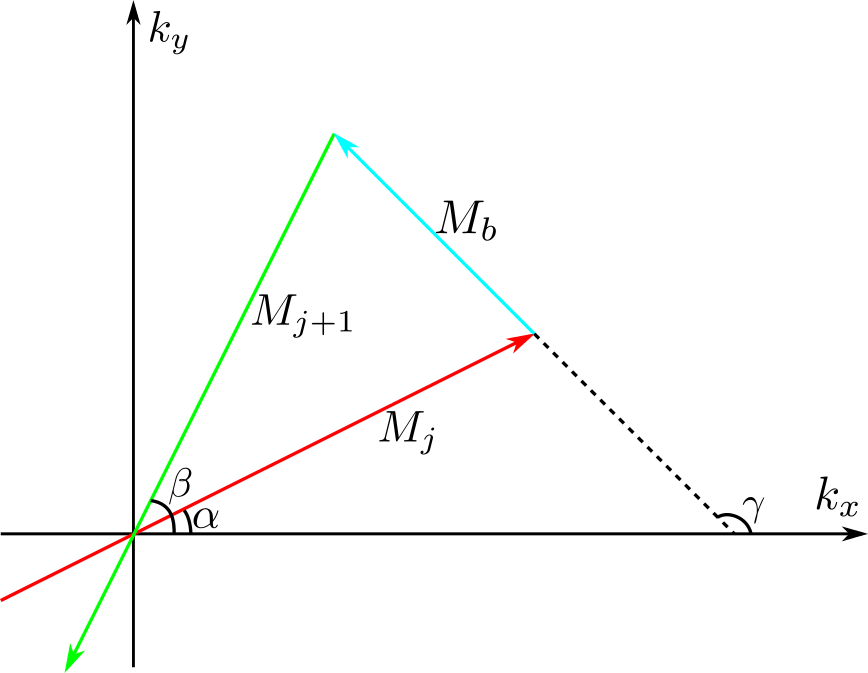
\includegraphics[width=0.50\textwidth]{fig/multi-echo-multi-spoke-blip.png}
  \caption{Illustration of the calculation of a blip gradient. (Red line) The $j^{\text{th}}$ echo with the angle $\alpha$ and gradient moment $M_{j}$ from the k-space center. (Green line) The $(j+1)^{\text{th}}$ echo with the angle $\beta$ and gradient moment $M_{j+1}$ to the k-space center. (Cyan line) The blip gradient with the angle $\gamma$ and gradient moment $M_{\text{b}}$.} \label{Fig:multi-echo-multi-spoke-blip}
\end{figure}
To implement MEMS, blip gradients on both readout axes have to be appropriately prepared. As illustrated in \cref{Fig:multi-echo-multi-spoke-blip}, $M_{j}$ and $M_{j+1}$ represent the gradient moment from the $j^{\text{th}}$ echo center and to the $(j+1)^{\text{th}}$ echo center, respectively. In the current sequence implementation, $M_{j} = M_{j+1} = M$. Moreover, the $j^{\text{th}}$ and $(j+1)^{\text{th}}$ echo has an angle of $\alpha$ and $\beta$, respectively. Similarly, $M_{\text{b}}$ is the gradient moment of the blip connecting the end of $j^{\text{th}}$ echo and the beginning of $(j+1)^{\text{th}}$ echo, and $\gamma$ is the angle of the blip. Thus, the following property holds
\begin{align}
  \vec{M}_{\text{b}}           &= \vec{M}_{j+1} - \vec{M}_{j} \\
  \Rightarrow M_{\text{b}} (x) &= M \cdot ( \cos \beta - \cos \alpha ) \\
  \Rightarrow M_{\text{b}} (y) &= M \cdot ( \sin \beta - \sin \alpha ) 
\end{align}
where $M_{\text{b}} = \sqrt{ M^2_{\text{b}} (x) + M^2_{\text{b}} (y) }$. Consequently, the duration of $M_{\text{b}}$ depends on the angle increment between two successive echoes and the gradient moments of $M_{j}$ and $M_{j+1}$. 


\begin{figure}[p]
  \centering
  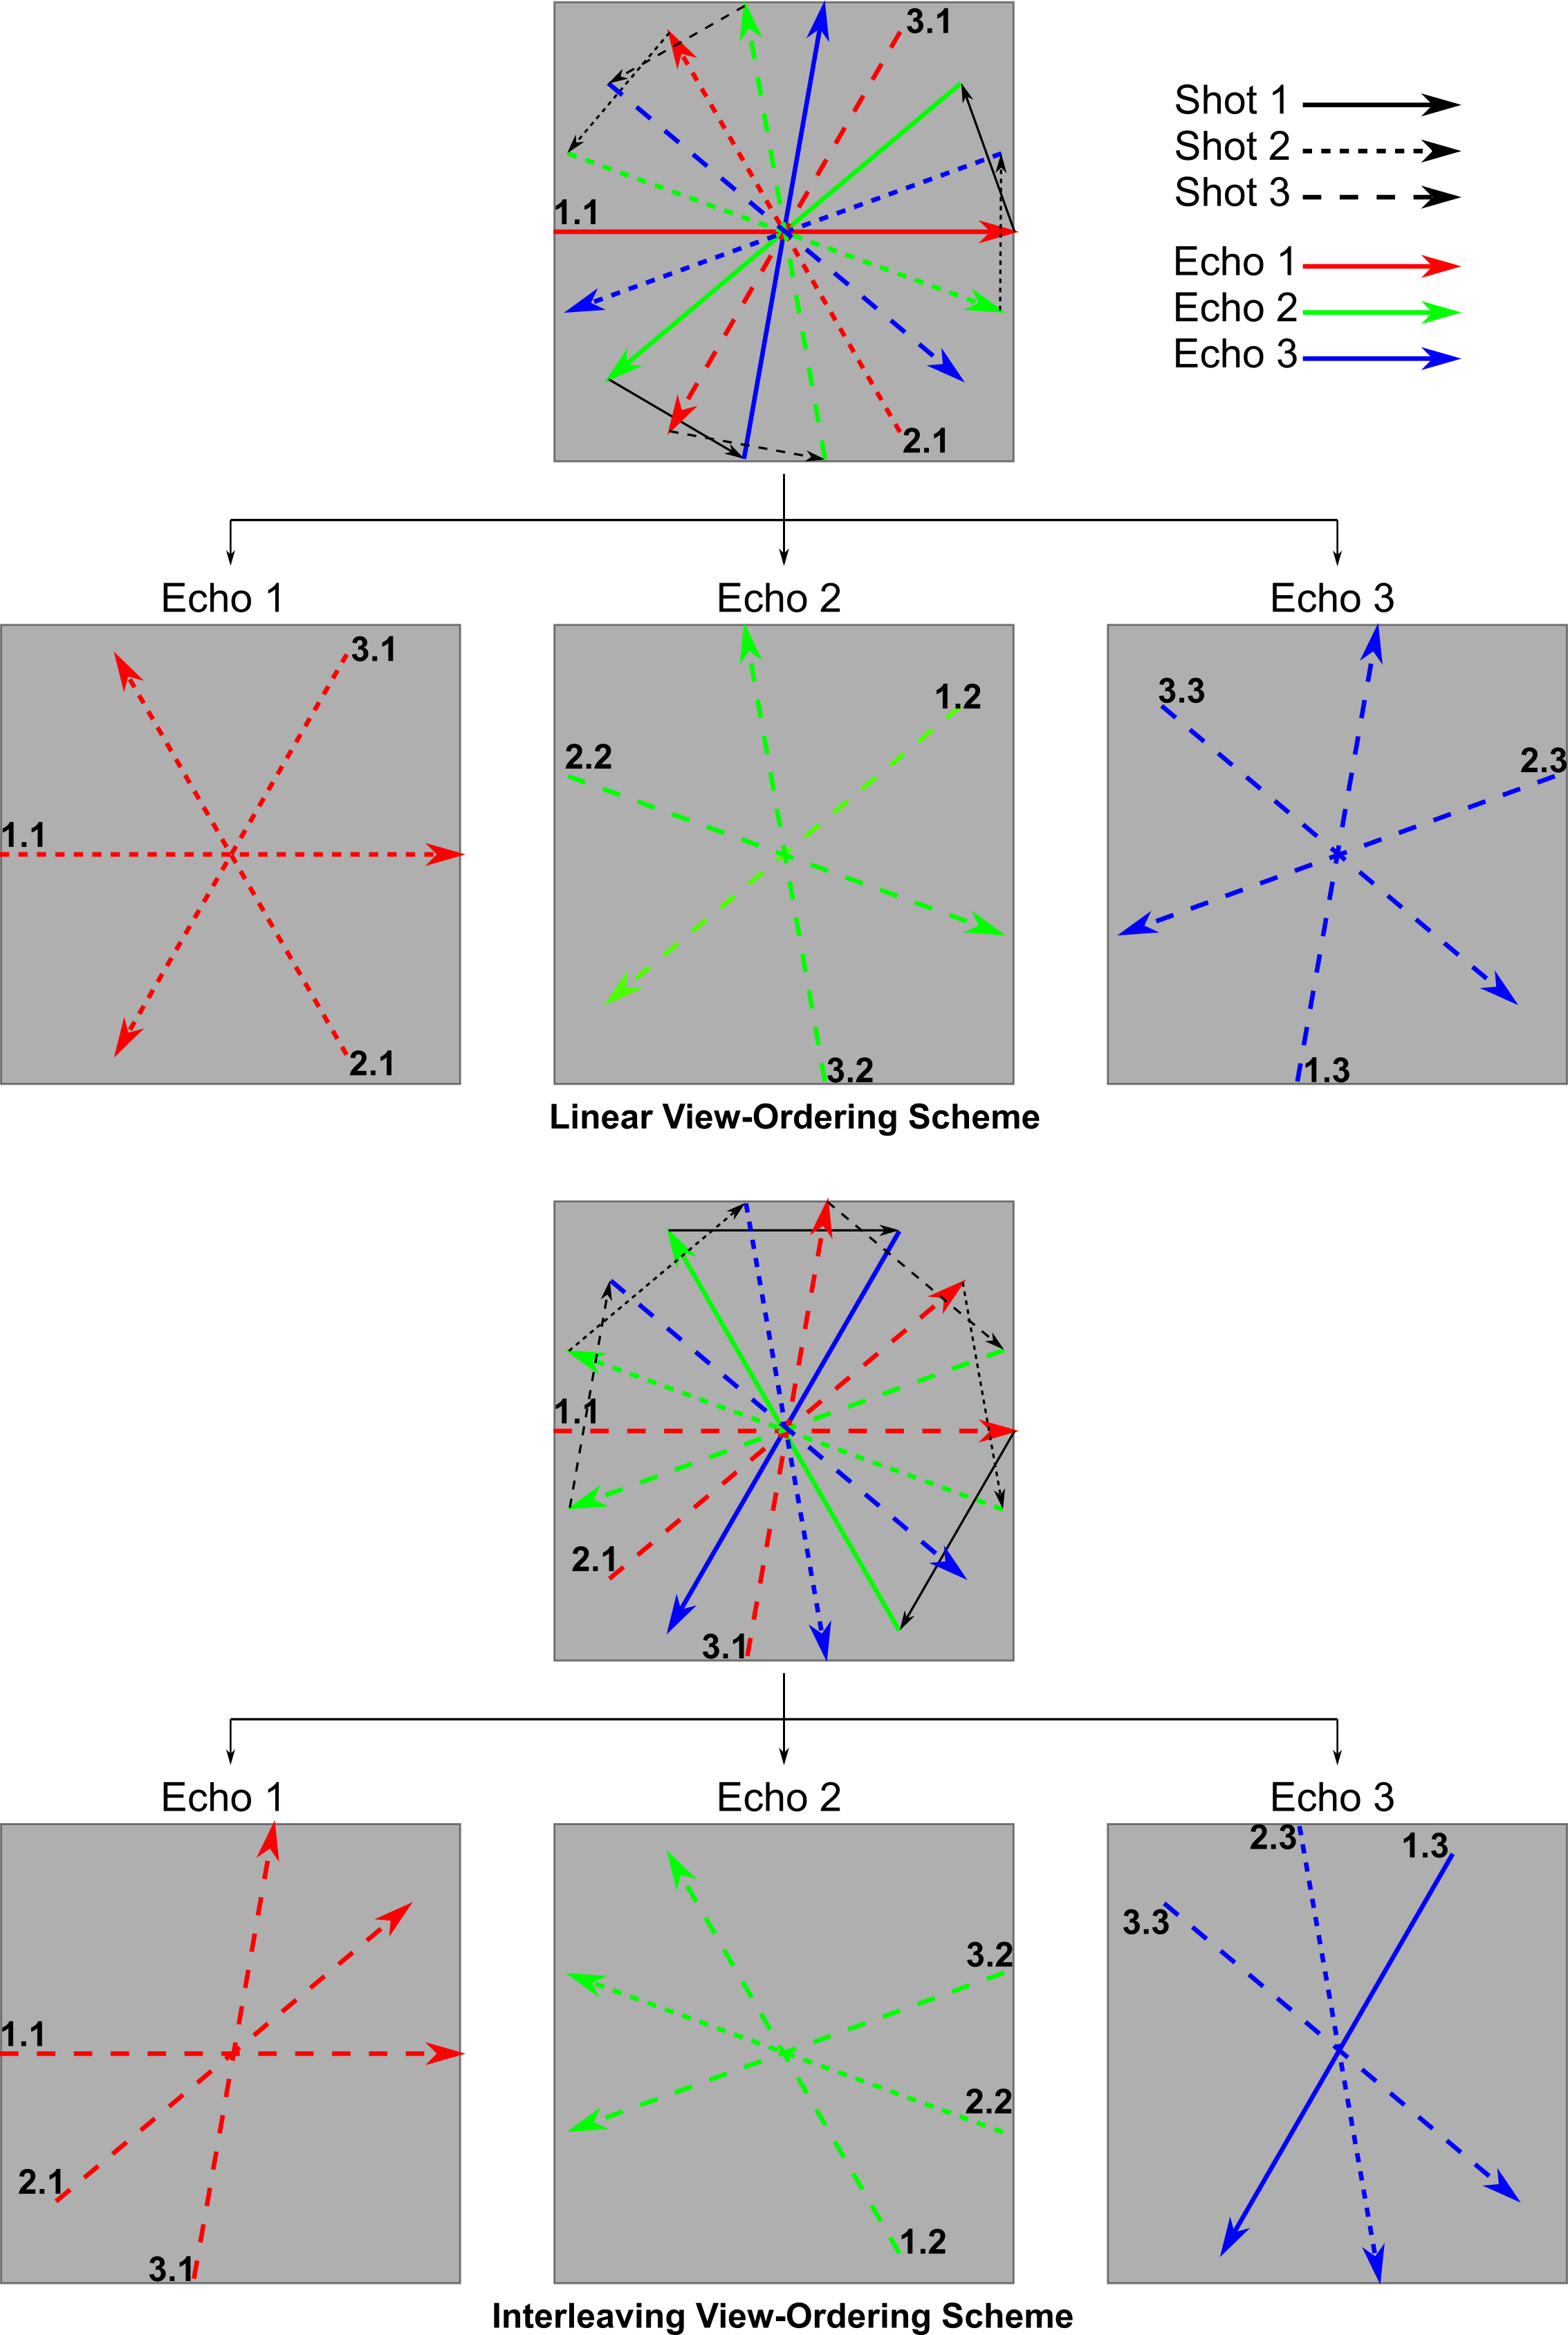
\includegraphics[width=0.90\textwidth]{fig/multi-echo-multi-spoke-vo.png}
  \caption{Schematic illustration of view-ordering schemes in MEMS, where one frame consists of \num{9} spokes, \num{3} shots (e.g.~excitations), and \num{3} echoes per shot. (Top) Linear. (Bottom) Interleaving. The index $k$.$l$ denotes the $l$\textsuperscript{th} echo in the $k$\textsuperscript{th} shot.} \label{Fig:multi-echo-multi-spoke-vo}
\end{figure}
There exist two common view-ordering schemes in MEMS, linear and interleaving, which correspond to sequential and star in \cite{2004_vo_rFSE}, respectively. Both schemes are depicted in \cref{Fig:multi-echo-multi-spoke-vo}. In \textbf{linear} view-ordering scheme, both echo trains and echoes after one excitation are sampled sequentially, while even echoes are reversed to achieve the shortest blip gradient. Thus, the spoke index $s$ corresponding to the $l^{\text{th}}$ echo in the $k^{\text{th}}$ shot is
\begin{equation} \label{Equ:mems-linear}
  s = (k-1) \cdot L + l
\end{equation}
which can then be inserted into \cref{Equ:rtmri-spk-ang} to calculate the angle of any echo. As shown in the top of \cref{Fig:multi-echo-multi-spoke-vo}, all spokes with the same echo index in linear view-ordering scheme are uniformly distributed in k-space and thus can be combined to an echo image. On the other hand, in \textbf{interleaving} view-ordering scheme, as shown in the bottom of \cref{Fig:multi-echo-multi-spoke-vo}, every echo train uniformly covers the k-space and interleaves with each other. Therefore, all spokes with the same echo index only cover partial k-space, which leads to non-uniformly distributed streaking artifacts when combined as one echo image. Instead, all echoes in one shot can be combined to one image with uniform k-space coverage. Here, the spoke index $s$ corresponding to the $l^{\text{th}}$ echo in the $k^{\text{th}}$ shot is
\begin{equation} \label{Equ:mems-interleaving}
  s = (l-1) \cdot K + k
\end{equation}
with $K$ being the total number of excitations per frame.

The view-ordering scheme of turns in MEMS can be the same as that discussed in \cref{Chp:rtMRI}, which, however, results in partial k-space coverage when summing spokes from all turns up. For linear view-ordering scheme, this can be overcome by adjusting the angle increment between two successive turns to $\Delta \theta_{\text{turn}} = 2\pi / (K \cdot N_T)$.


\subsection{Image Reconstruction} \label{Sec:me-theory-reco}
The signal model in multi-gradient-echo imaging can be written as
\begin{equation} \label{Equ:me-signal}
  y_{j,l}(t) = \int_{\vec{r}} \rho(\vec{r}) \cdot e^{- z(\vec{r}) \cdot \text{TE}_l} \cdot c_{j}(\vec{r}) \cdot e^{-i 2\pi \cdot \vec{k}_{l}(t) \cdot \vec{r}} \text{d}\vec{r} \quad \text{with} \; j \in [1,N],\; l \in [1,L]
\end{equation}
where $z(\vec{x}) = R_2^* (\vec{x}) + i \cdot 2\pi\cdot \Delta f (\vec{x})$ with the relaxation rate $R_2^* (\vec{x})$, the reciprocal of $T_2^* (\vec{x})$, and the off-resonance frequency map $\Delta f(\vec{x})$. As an extension from \cref{Equ:mri-pi-forward}, therefore, the corresponding forward signal model of the $l^\text{th}$ echo acquired via the $j^\text{th}$ coil is denoted as
\begin{align} 
  F_{j,l} (x) &= P_l \mathcal{F} \{\rho \cdot e^{- z \cdot \text{TE}_l} \cdot c_j \} \label{Equ:me-fwd-z} \\
              &= P_l \mathcal{F} \{\rho_l \cdot c_j \} \label{Equ:me-fwd-rho_l}
\end{align}
with $\rho$ being the proton density and $\rho_l$ being the $l^\text{th}$ echo image. It indicates two possibilities of image reconstruction for multi-gradient-echo imaging. The first one is to directly reconstruct the proton density $\rho$ and the $z$ map from the acquired multi-echo multi-coil data based on the forward model in \cref{Equ:me-fwd-z}, which requires a complicated model-based reconstruction technique, while the second one, as shown in \cref{Equ:me-fwd-rho_l}, reconstructs $L$ echo images, accomplished by an extended version of the standard NLINV \cite{2008_NLINV,2010_NLINV_Heart,2010_20ms_Uecker}. The extended NLINV for multi-echo data assumes that all echoes acquired in one image frame shares one set of coil sensitivity maps, so the cost function associated with the forward operator in \cref{Equ:me-fwd-rho_l} is
\begin{equation} \label{Equ:me_GN_cost}
  \norm{y-F(x)}_2^2 + \alpha \norm{W(x)}_2^2 \quad \text{with} \; x = \left( \begin{array}{c} 
  \rho_1 \\
  \vdots \\
  \rho_L \\
  c_1    \\
  \vdots \\
  c_N
  \end{array} \right) \quad .
\end{equation}
To minimize this cost function, both the Frech\'et derivative of the forward operator $DF(x)$ and the adjoint of the Frech\'et derivative $DF^H (x)$ are needed, which can be derived according to the forward operator in \cref{Equ:me-fwd-z},
\begin{align}
  DF_{j,l}(x) \left( \begin{array}{c}
    \text{d} \rho_1 \\
    \vdots \\
    \text{d} \rho_L \\
    \text{d} c_1 \\
    \vdots \\
    \text{d} c_N
  \end{array} \right) 
  &= P_{l} \mathcal{F} \{c_j \cdot \text{d} \rho_l + \rho_l \cdot \text{d} c_j) \} \\
  &= \text{d} y_{j,l} \\
\intertext{and}
  DF^{H}(x) \left( \begin{array}{c}
    \text{d} y_{1,1} \\
    \vdots \\
    \text{d} y_{N,L}
  \end{array} \right) 
  &= \left( \begin{array}{c}
    \sum_{j=1}^{N} c_j^* \cdot \mathcal{F}^{-1} \{ P_1^H \text{d} y_{j,1} \} \\
    \vdots \\
    \sum_{j=1}^{N} c_j^* \cdot \mathcal{F}^{-1} \{ P_L^H \text{d} y_{j,L} \} \\
    \sum_{l=1}^{L} \rho_l^* \cdot \mathcal{F}^{-1} \{ P_l^H \text{d} y_{1,l} \} \\
    \vdots \\
    \sum_{l=1}^{L} \rho_l^* \cdot \mathcal{F}^{-1} \{ P_l^H \text{d} y_{N,l} \} 
  \end{array} \right) \\
  &= \left( \begin{array}{c}
    \text{d} \rho_1 \\
    \vdots \\
    \text{d} \rho_L \\
    \text{d} c_1 \\
    \vdots \\
    \text{d} c_N
  \end{array} \right) \quad .
\end{align}

This multi-echo NLINV (dubbed as meNLINV) reconstruction fits perfectly into the MESS sampling scheme, comprising $L$ echo images acquired by spokes with the same orientations in every image frame, because the assumption of a common set of coil sensitivity maps ensures the linearity of off-resonance phase evolution along echo images. meNLINV is applicable to MEMS as well. In MEMS, however, one image can also be reconstructed via the standard NLINV when all spokes acquired in one frame are combined together, regardless of their respective echo numbers. Noteworthy, the $L$ echo images in MEMS can be combined as one single image after the meNLINV reconstruction. The simplest combination is to sum all these echo images up, resulting in a somewhat off-resonance ``average" image. A better combination with off-resonance correction is introduced as following.

\subsection{Off-Resonance Estimation and Correction} \label{Sec:me-iORC}
As shown in \cref{Equ:me-fwd-z,Equ:me-fwd-rho_l}, the signal model along echo images is $\rho_l = \rho \cdot e^{- (R_2^* + i \cdot 2\pi \cdot \Delta f) \cdot \text{TE}_l}$. Given the reconstructed echo images $\rho_l$, quantitative parameter maps $\rho$, $R_2^*$, and $\Delta f$ can be obtained via a pixel-wise fitting. Thus, a combined image with off-resonance correction (\acs{ORC}) can be obtained via conjugate phase reconstruction,
\begin{equation} \label{Equ:me_cp}
  \rho_{\text{comb}} = \sum_{l=1}^{L} \rho_l \cdot e^{+ i \cdot 2\pi \cdot \Delta f \cdot \text{TE}_l} \quad .
\end{equation}
The quality of the combined image depends on the quality of the estimated off-resonance frequency map, which can potentially be improved by regularized field map estimation (e.g.~see \cite{2004_fim_est_spiral,2008_fim_est}) or even a model-based reconstruction (e.g.~see \cite{2008_r2s_fm_fMRI,2009_fim_t2s_me_TMI}) based on the signal model in \cref{Equ:me-fwd-z}. 


\section{Methods} \label{Sec:me-method}

\subsection{Multi-Echo Radial FLASH Data Acquisition}
Five young healthy volunteers were recruited for multi-echo radial FLASH studies. Written informed consent, according to the recommendations of the local ethics committee, was obtained from all volunteers before experiments.

This work presents phantom and \textit{in-vivo} studies conducted at \SI{3}{\tesla} (MAGNETOM Prisma, Siemens Healthcare, Erlangen, Germany). The \num{64}-channel head coil is used for the phantom and brain studies, while human cardiac imaging is measured by combining \num{32}-element thorax coil with \num{18} elements of the spine coil. All studies employ \num{5} sequential turns.

\subsubsection*{Phantom}
A standard multi-purpose resolution phantom from the vendor is used to validate both MESS and MEMS sequences with acquisition parameters: RF spoiling, \ang{8} flip angle, \SI{232}{\mm} \acs{FOV}, \SI{1.81}{\mm} in-plane resolution, \SI{6}{\mm} slice thickness, \num{128} base resolution, \num{45} excitations per image frame and \num{9} echoes acquired after each excitation. This yields \num{45} spokes per echo image and \num{9} echo images per frame in MESS, but a total of \num{405} spokes per frame in MEMS. Linear view-ordering scheme is used in MEMS. \SI{1.15}{\ms} \acs{TE}\textsubscript{1}, \SI{0.97}{\ms} ESP, and \SI{9.45}{\ms} and \SI{9.63}{\ms} TR in MESS and MEMS, respectively.

\subsubsection*{Brain}
MEMS radial FLASH with linear view-ordering scheme on the human brain is studied to demonstrate its applicability in $T_2^*$-weighted imaging with acquisition parameters: RF spoiling, \ang{8} flip angle, \SI{224}{\mm} FOV, \SI{1.0}{\mm} in-plane resolution, \num{224} base resolution, \SI{4}{\mm} slice thickness, \SI{2.22}{\ms} TE\textsubscript{\num{1}}, \SI{2.74}{\ms} ESP, \SI{42.5}{\ms} TR, \num{25} excitations per image frame and \num{15} echoes acquired after each excitation. Therefore, in total \num{375} spokes are sampled for one image frame and every echo comprises \num{25} spokes. The over-gridding ratio is set to \num{1} due to large numbers of samples per spoke.

\subsubsection*{Cardiac}
To apply MEMS radial FLASH with linear view-ordering scheme into real-time cardiac imaging, the data acquisition must be fast enough to capture cardiac motions. Hence, \num{3} echoes are acquired per RF excitation, and the number of spokes per frame vary from \num{33} to \num{27}, \num{21}, and \num{15}, leading to temporal resolutions of \SI{49}{\ms}, \SI{40}{\ms}, \SI{33}{\ms}, and \SI{24}{\ms} with the corresponding echo times and repetition time TE\textsubscript{\num{1}}/TE\textsubscript{\num{2}}/TE\textsubscript{\num{3}}/TR $=$ \num{1.22}/\num{2.45}/\num{3.69}/\SI{4.43}{\ms}, \num{1.22}/\num{2.49}/\num{3.77}/\SI{4.56}{\ms}, \num{1.22}/\num{2.53}/\num{3.85}/\SI{4.64}{\ms}, and \num{1.22}/\num{2.57}/\num{3.95}/\SI{4.74}{\ms}, respectively. The other acquisition parameters are RF spoiling, \ang{8} flip angle, \SI{256}{\mm} FOV, \SI{1.6}{\mm} in-plane resolution, \SI{4}{\mm} slice thickness, and \num{160} base resolution.

\subsection{Image Reconstruction}
As discussed in \cref{Sec:mri_grid}, Gridding \& FFT in combination with square root of sum of squares of all coils is used as the basic reconstruction method for validation. Moreover, three types of NLINV are available for multi-echo data (see \cref{Sec:me-theory-reco}): standard NLINV,  meNLINV with a subsequent summation of all echo images, and meNLINV with a subsequent summation of all echo images corrected for off-resonance effects. The development of the advanced model-based image reconstruction for multi-echo data, however, is beyond the scope of this thesis.

The Gridding \& FFT algorithm used the Gridding functions developed in C by Hargreaves\footnote{\url{http://mrsrl.stanford.edu/~brian/gridding/}}, while the standard NLINV and meNLINV are implemented on a single graphics processing unit (GeForce GTX \num{580}, NVIDIA, Santa Clara, CA) by Uecker. The off-resonance estimation relies on the pixel-wise fitting is implemented via the nlinfit function in MATLAB. All reconstructions are performed offline after data acquisitions. Due to reduced spokes in the echo image reconstructions of cardiac data, \num{7} Newton steps are employed, while all other studies use \num{6} Newton steps. The reconstruction on the very first maps is initialized with $\rho_l = 1$, and $c_j = 0$, and the standard temporal regularization with a damping factor of \num{0.9} is used. Parameter for the preconditioning matrix are the same as described in \cref{Sec:rtmri-nlinv}. Temporal median filter and denoising filter are not used after image reconstruction in this study.


\section{Results}

\begin{figure}[tb]
  \centering
  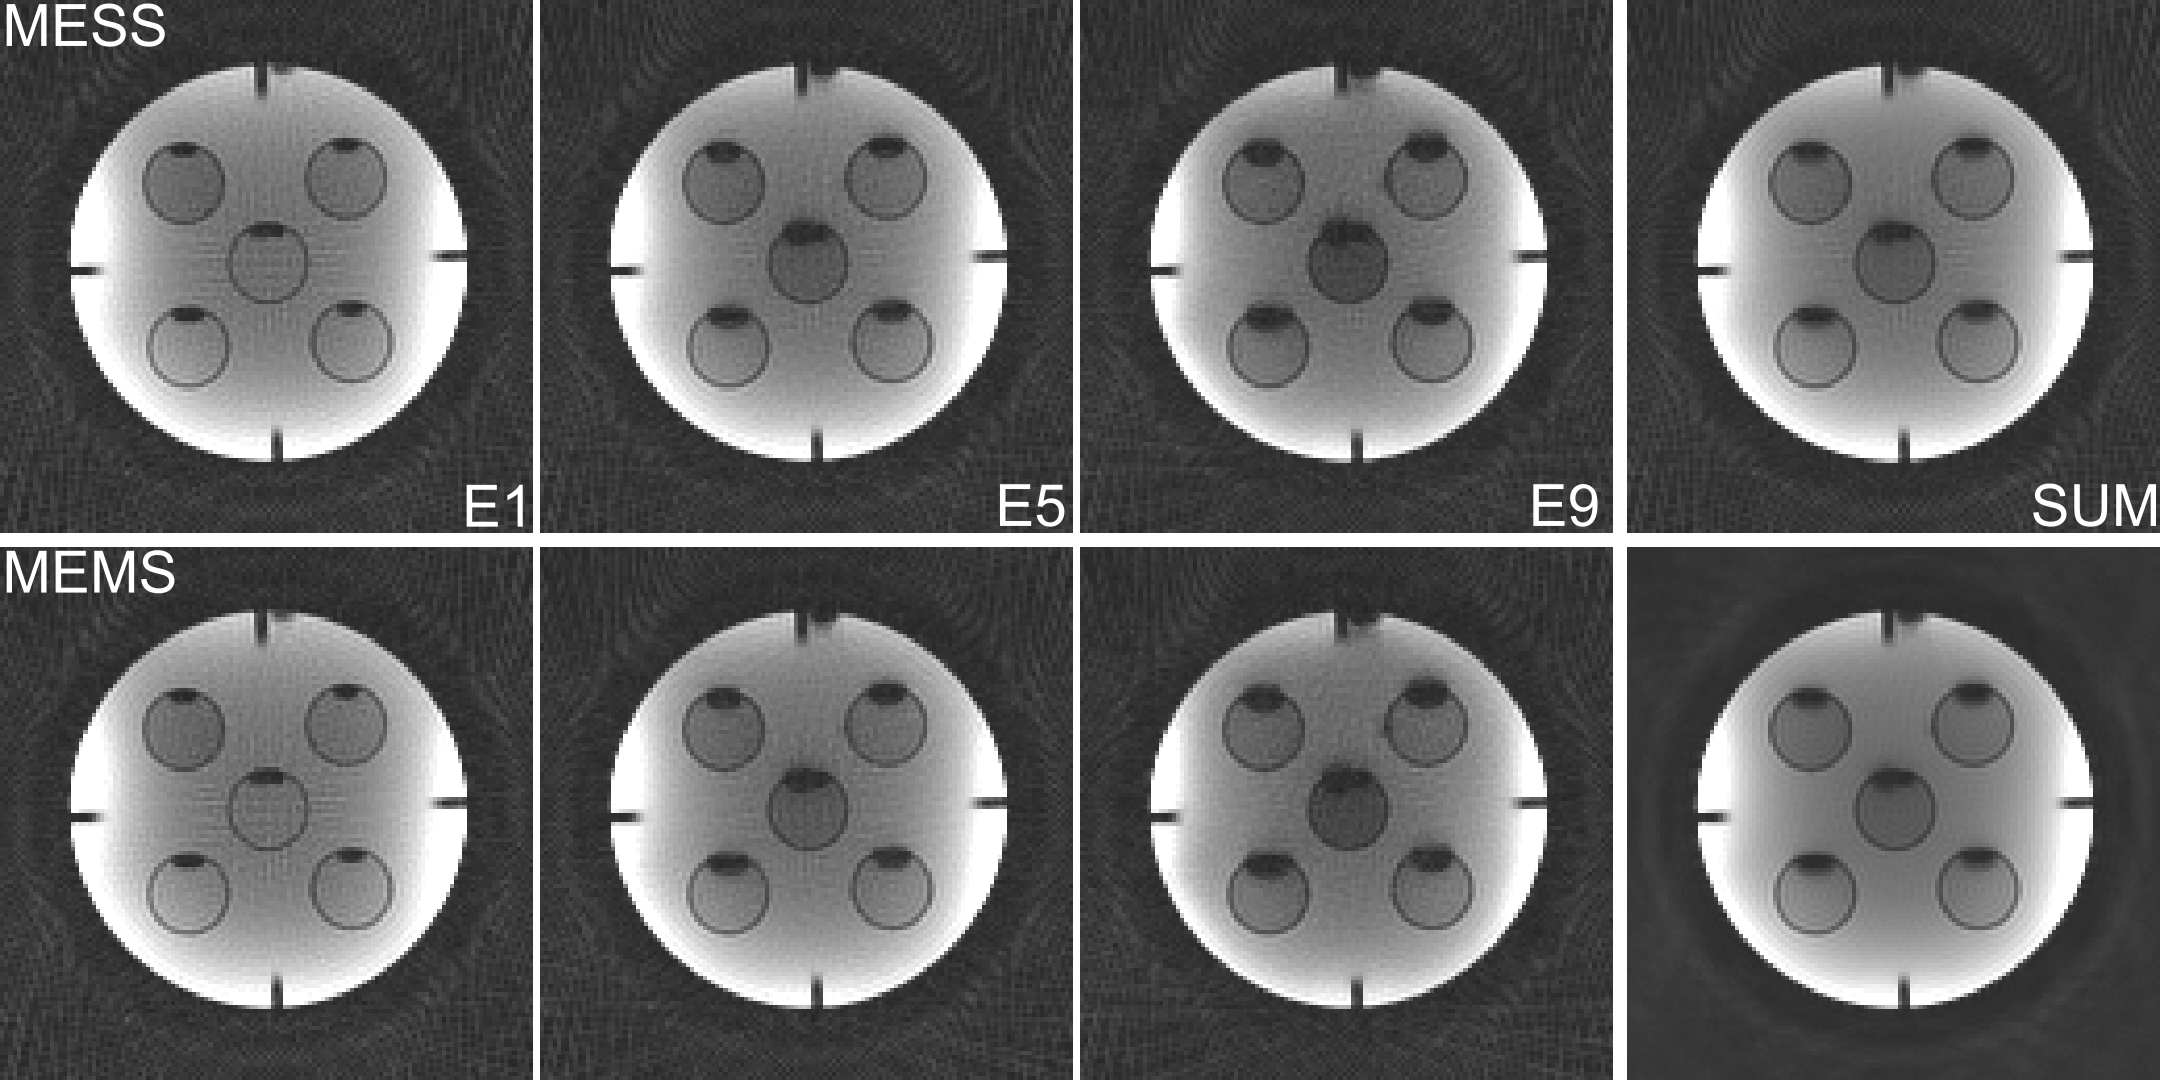
\includegraphics[width=\textwidth]{fig/multi-echo-pha-grid.png}
  \caption{Multi-echo images reconstructed by Gridding \& FFT. The acquisition parameters were described in \cref{Sec:me-method}. The first row represents the \nth{1}, \nth{5}, and \nth{9} echo image, and the complex sum of all echoes from left to right from data acquired by MESS, while the second row represents the corresponding images from MEMS.} \label{Fig:multi-echo-pha-grid}
\end{figure}
\subsection{Validation Studies}
As shown in \cref{Fig:multi-echo-pha-grid}, both MESS and MEMS acquisitions yield similar echo images reconstructed by the Gridding \& FFT reconstruction, which directly validates the appropriate switching of gradients in MEMS. Moreover, TE increases along echoes, and so do the $T_2^*$ weighting and off-resonance phase modulation. This not only matches the signal model in \cref{Equ:me-fwd-z}, but also can be seen in the displayed echo images, where the signal intensity of the five small tubes substantially decreases and the sizes of the black air bubbles on top of every tube enlarges from the \nth{1} to \nth{9} echo. On the other hand, as all echo images from MESS are acquired by spokes with the same orientations, the summation of all echo images gives no benefit. However, the spoke orientation differs among echoes in MEMS, and thus the summation of all echo images contains $L$-fold number of spokes, thereby improving the SNR and reducing streaking artifacts caused by radial undersampling. 


\subsection{Human Studies}

\begin{figure}[p]
  \centering
  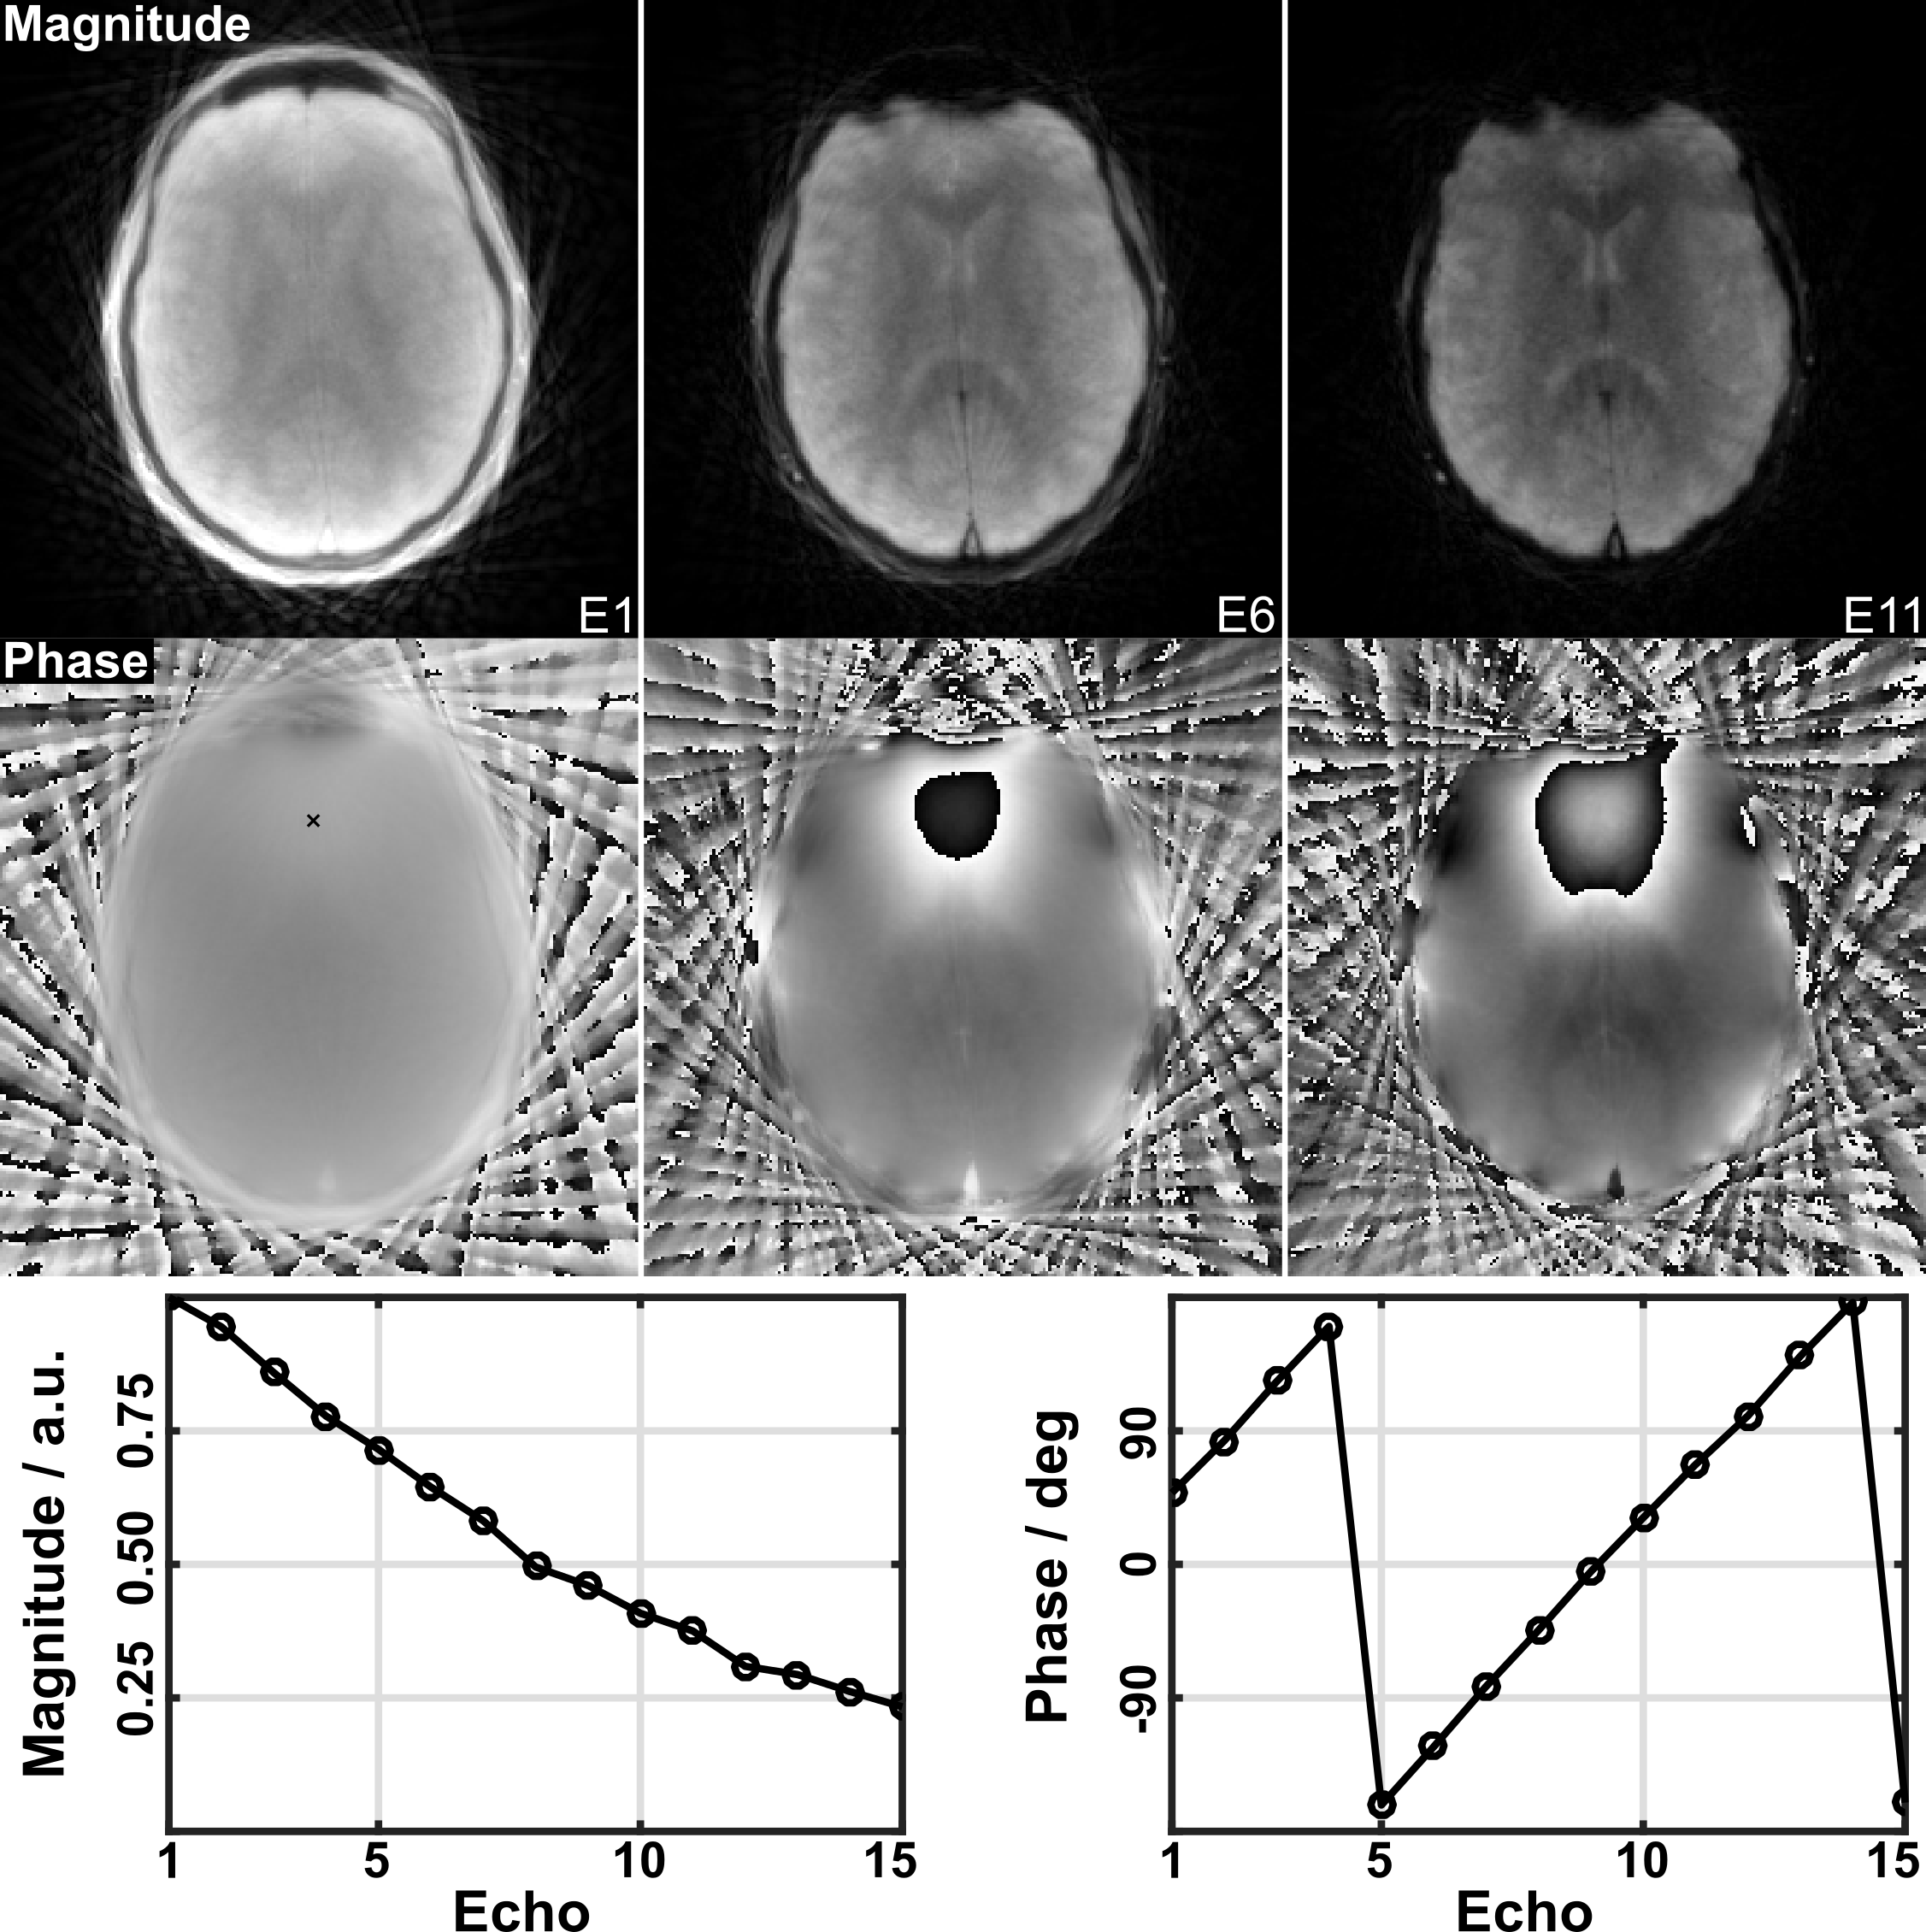
\includegraphics[width=\textwidth]{fig/multi-echo-brain-menlinv.png}
  \caption{Multi-echo brain images reconstructed by meNLINV. The acquisition parameters were described in \cref{Sec:me-method}. The image panels represent (top) magnitudes and (middle) phases of the (left) \nth{1}, (center) \nth{6}, and (right) \nth{11} echo. (Bottom) The curve panels represent (left) normalized magnitude and (right) phase evolution along echoes in the marked pixel on the phase map of the \nth{1} echo.} \label{Fig:multi-echo-brain-menlinv}
\end{figure}
\subsubsection*{Brain}
Similar to MESS, MEMS radial FLASH with linear view-ordering scheme can also be reconstructed by meNLINV, yielding $L$ echo images and one set of coil sensitivities for each frame. \cref{Fig:multi-echo-brain-menlinv} shows three representative echo images (the \nth{1}, \nth{6}, and \nth{11} echo). With relatively short TE and long TR, the \nth{1} echo image exhibits PD-weighted image contrasts. As TE increases, the white matter becomes grayer and the overall intensity drops, indicating heavier $T_2^*$ weighting. Moreover, signal void emerges and enlarges along echoes in the frontal brain area because of air-induced off-resonance effects. This can be clearly seen in the phase images, where off-resonance frequencies linearly increase with echo time. Quantitative analysis is given in the bottom panel of \cref{Fig:multi-echo-brain-menlinv}, containing both the normalized magnitude and the phase evolution along echoes in the marked pixel, representing the $T_2^*$ signal decay and off-resonance phase modulation, respectively. Again, the signal change in these curves matches the multi-echo signal model in \cref{Equ:me-fwd-z}. 

Further, the results shown in \cref{Fig:multi-echo-brain-menlinv} confirm the rationale of the meNLINV reconstruction method, which assumes that all echoes acquired in one frame share one set of coil sensitivity maps. This assumption ensures the linearity of the phase evolution induced by off-resonance along echoes. On the other hand, in the single-echo NLINV that reconstructs echoes independently, coil sensitivity maps have to be either combined with the echo image after reconstruction in order to exclude the possibility that phases caused by off-resonance may partially remain in coils, or kept fixed among echoes where coils are estimated from the first echo. Therefore, meNLINV can also be applied to phase-contrast flow MRI data, and phase-contrast maps can be directly calculated between the reconstructed images without the need of adding coils back as in \cref{Equ:rtmri-pc-rho-coil}. 

\begin{figure}[p]
  \centering
  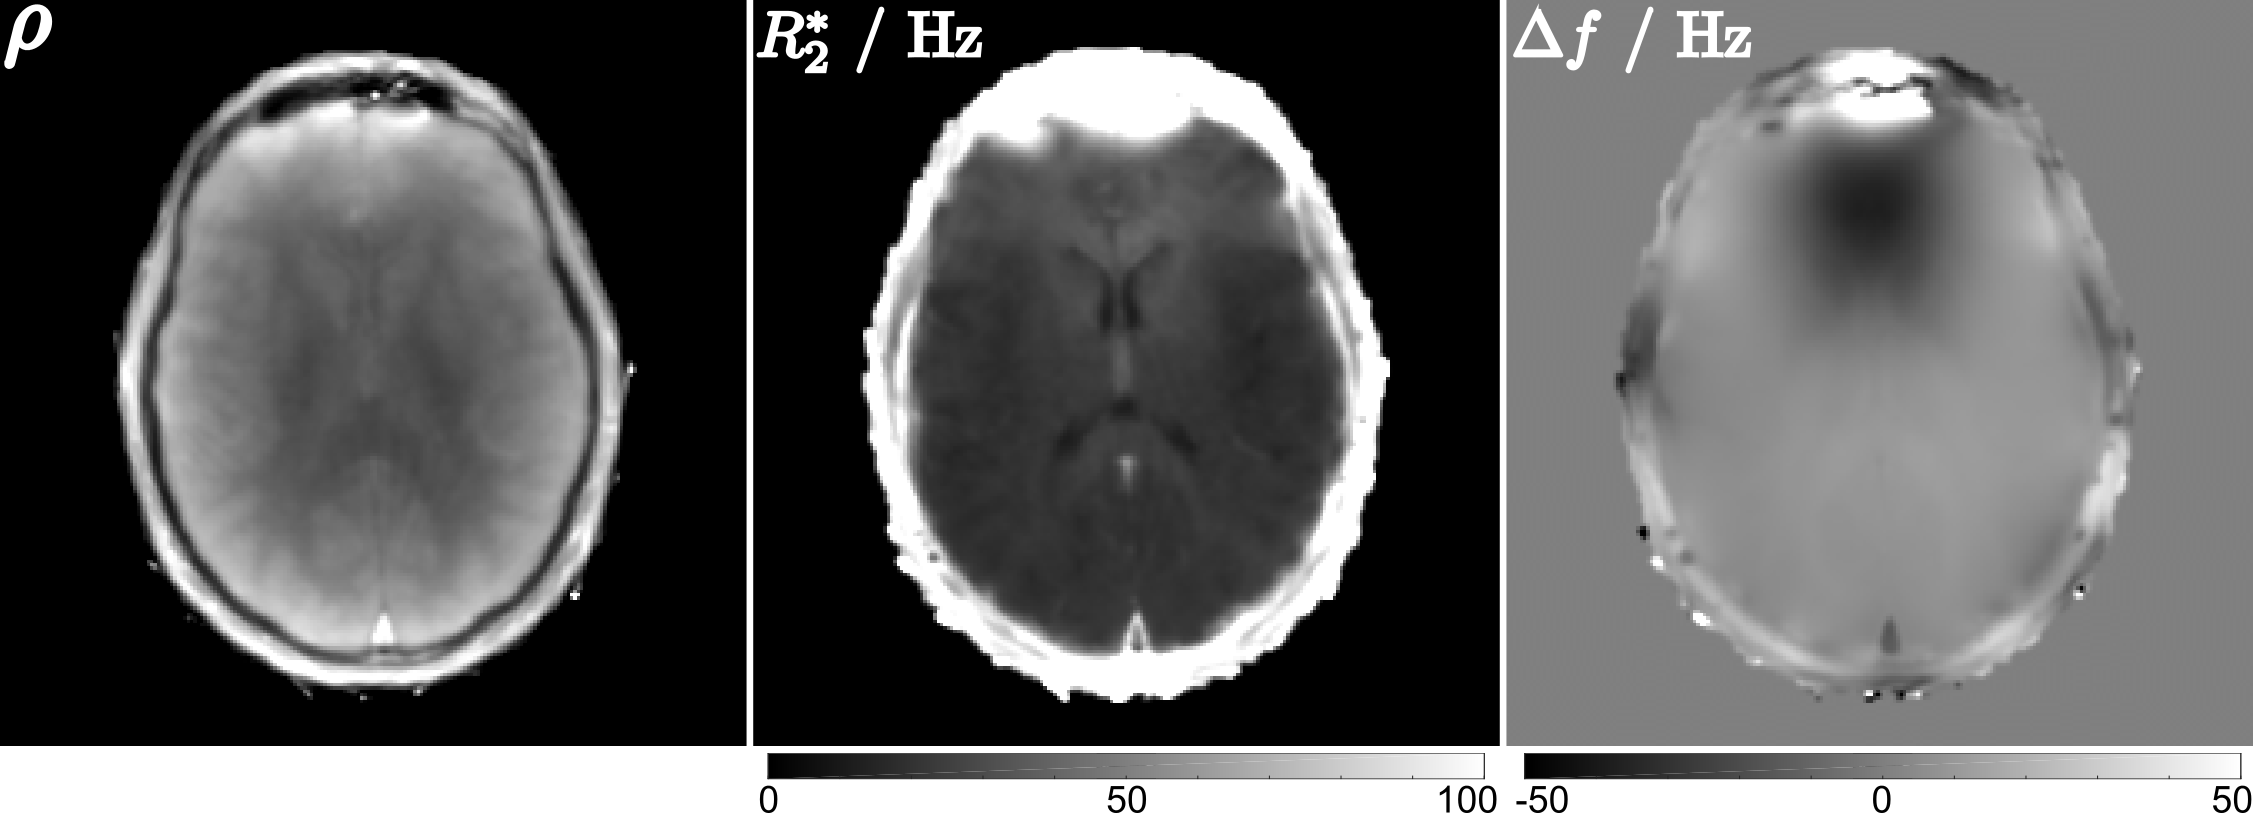
\includegraphics[width=\textwidth]{fig/multi-echo-brain-menlinv-iORC.png}
  \caption{Off-resonance estimation with echo images reconstructed by meNLINV. Pixel-wise fitting yields three quantitative parameter maps: (left) proton density $\rho$, (center) relaxation rate $R_2^*$, and (right) off-resonance frequency $\Delta f$.} \label{Fig:multi-echo-brain-menlinv-iORC}
  
  \par\bigskip
  
  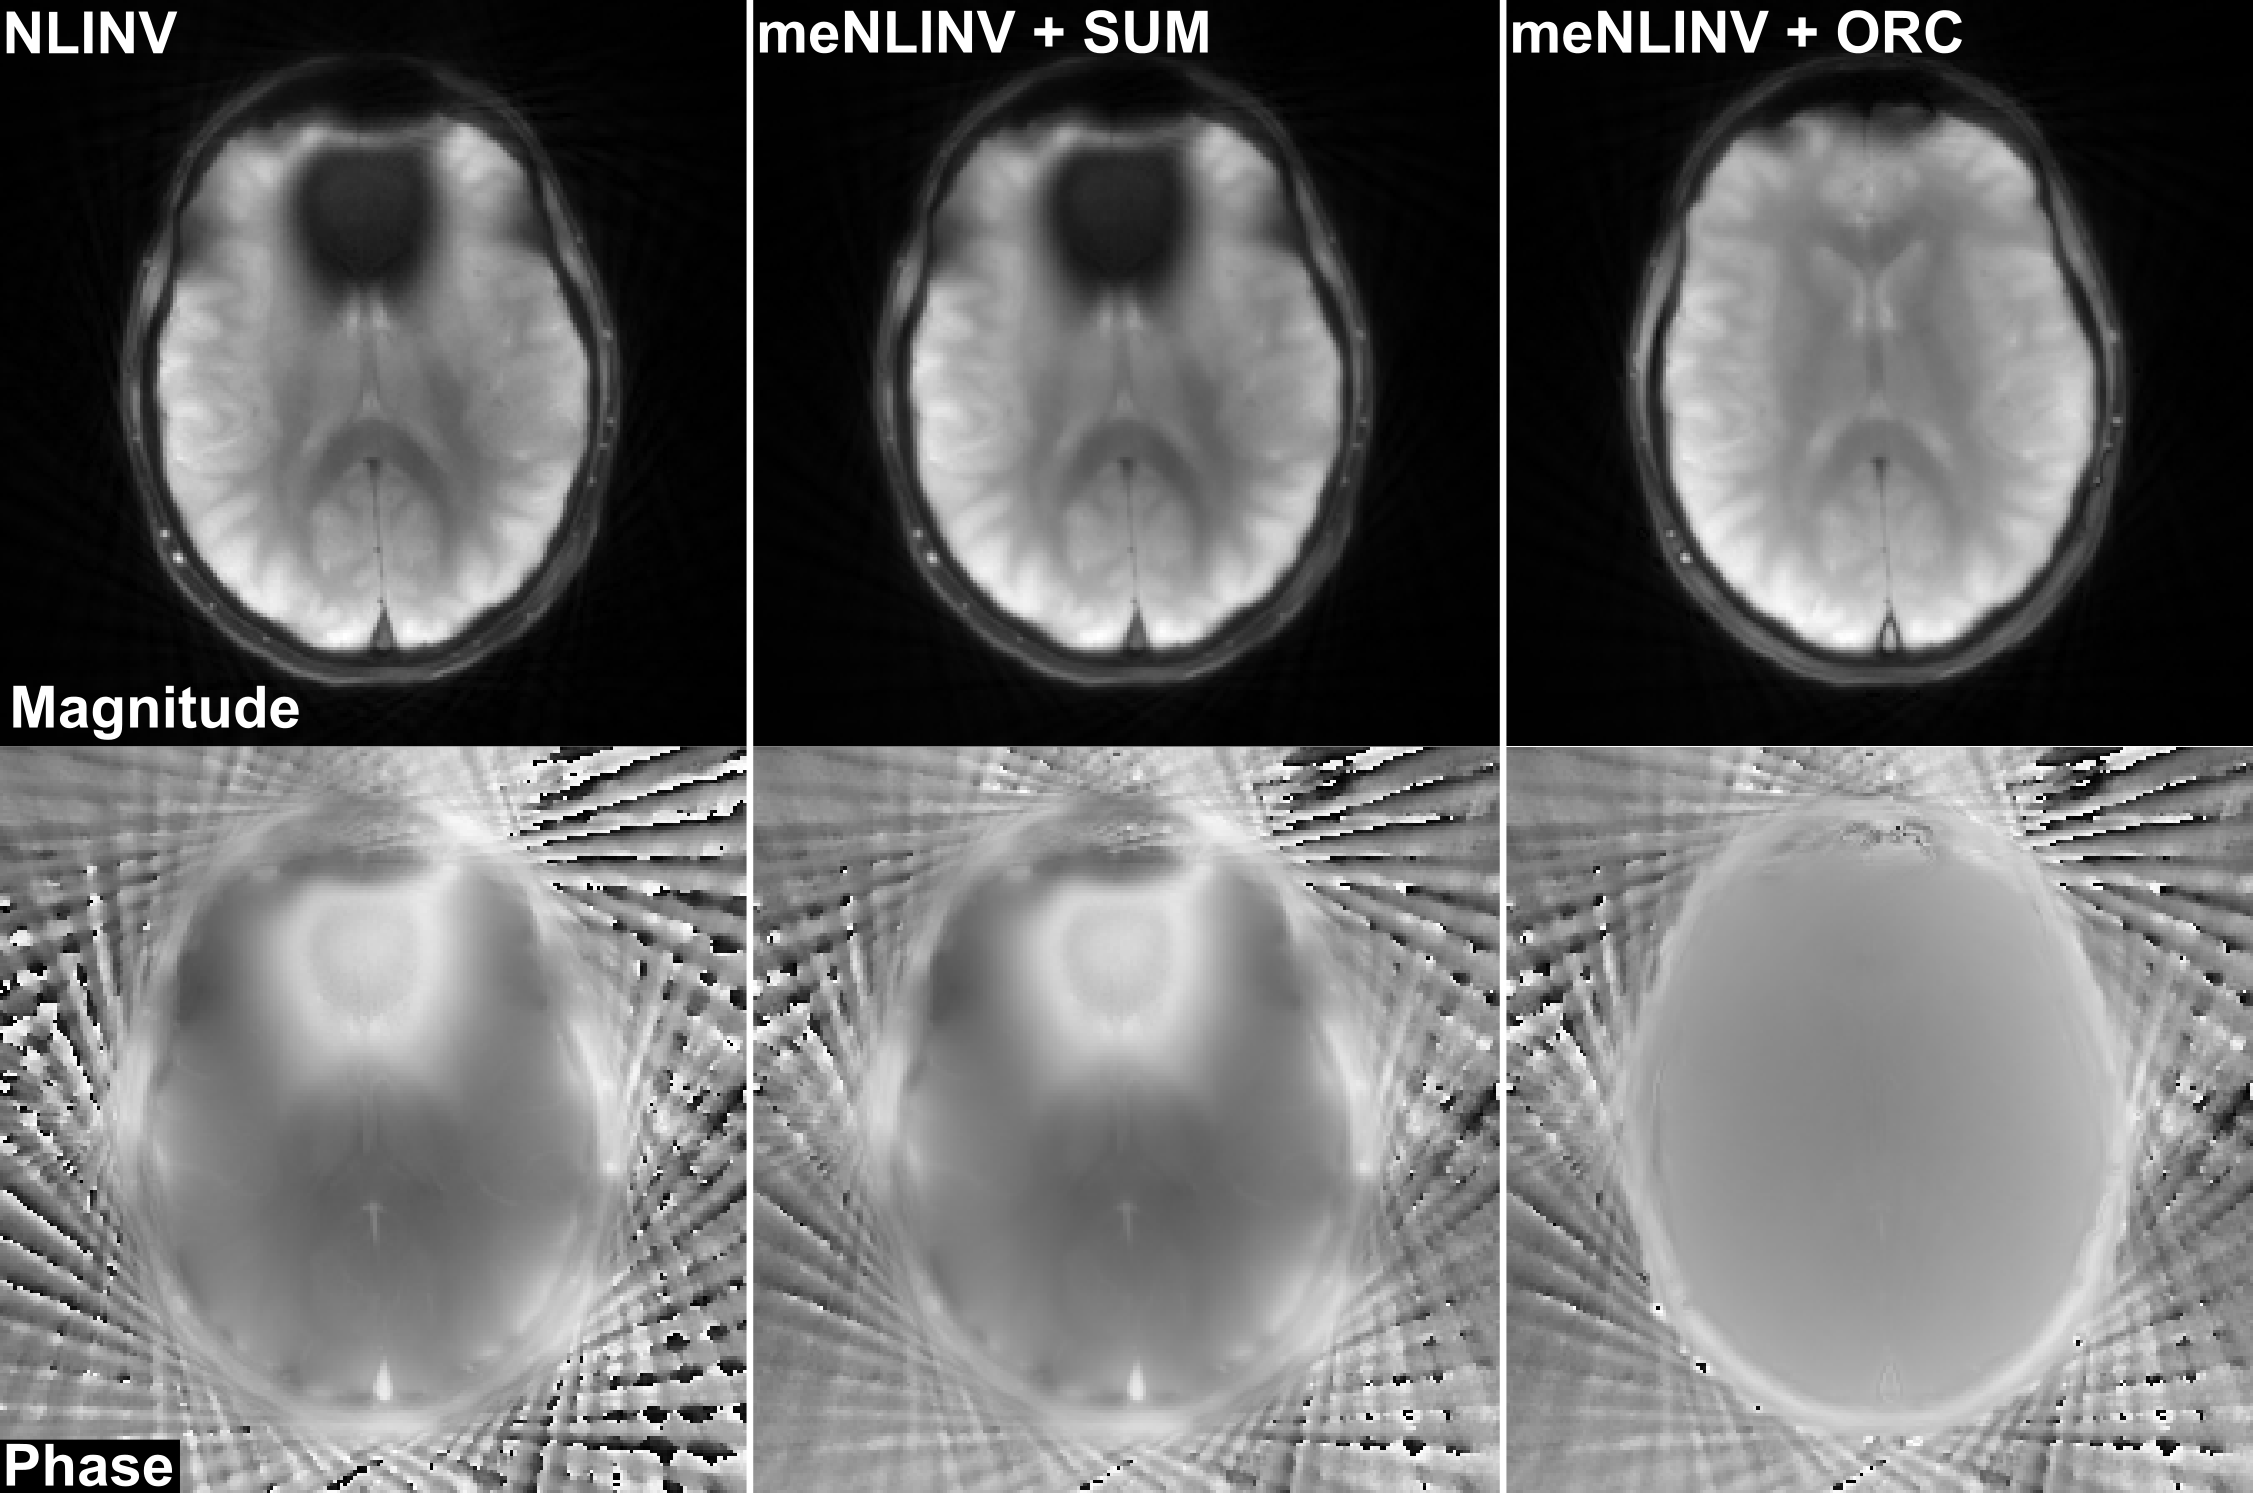
\includegraphics[width=\textwidth]{fig/multi-echo-brain-reco-comp.png}
  \caption{Comparisons of (top) magnitude and (bottom) phase images reconstructed by three types of NLINV-based methods: (left) standard NLINV that reconstructs all echoes acquired in one frame once, (center) meNLINV with a subsequent summation of all echo images, and (right) meNLINV with off-resonance correction.} \label{Fig:multi-echo-brain-reco-comp}
\end{figure}
With all the reconstructed echo images and echo times, the pixel-wise fitting procedure described in \cref{Sec:me-iORC} yields three quantitative maps (the proton density $\rho$, the relaxation rate $R_2^*$, and the off-resonance frequency $\Delta f$), as shown in \cref{Fig:multi-echo-brain-menlinv-iORC}. Afterwards, off-resonance correction can be performed to obtain a pure $T_2^*$-weighted image, as shown in the right of \cref{Fig:multi-echo-brain-reco-comp}. Even though signal void appears in multi-echo radial sampling methods, the spatial information of the scanned subject is well maintained. Spatial distortion, however, is commonly seen in multi-echo Cartesian sampling (e.g.~EPI). More importantly, when compared to images reconstructed by the (left) standard NLINV and (center) meNLINV with a subsequent summation of all echo images, the off-resonance corrected image is mostly not contaminated by signal void due to off-resonance phase modulation.

\subsubsection*{Cardiac}
\begin{figure}[tb]
  \centering
  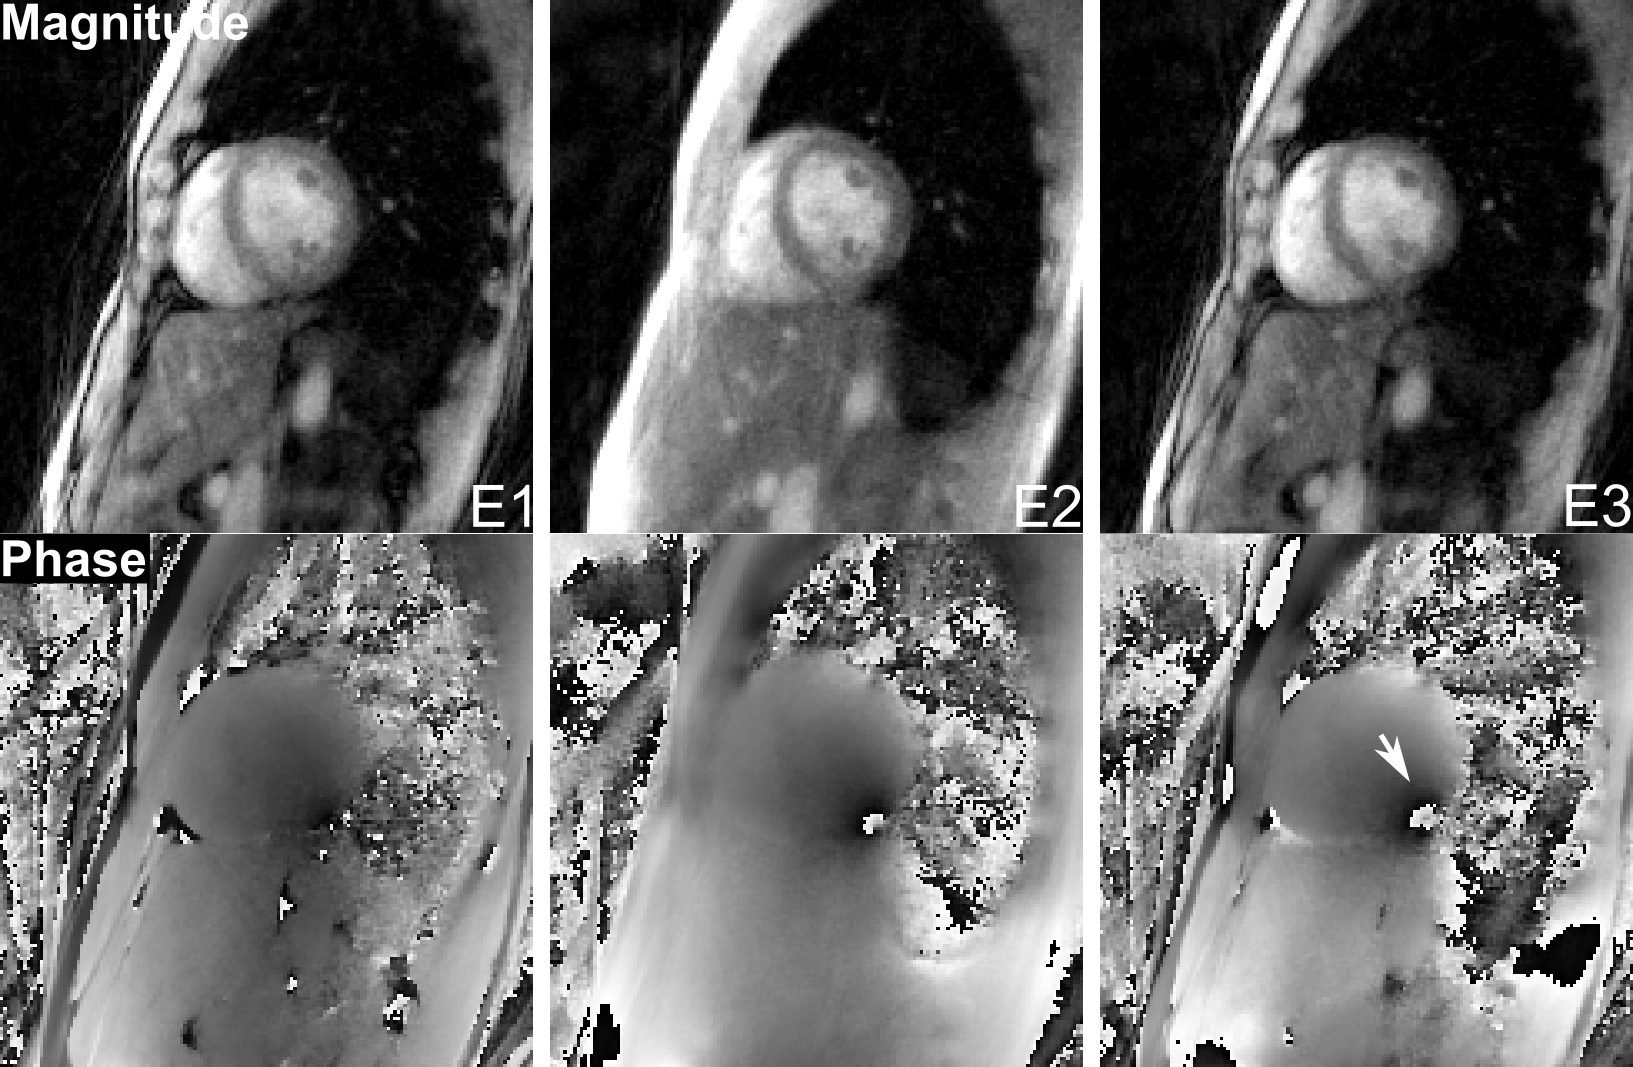
\includegraphics[width=\textwidth]{fig/multi-echo-cardiac-menlinv.png}
  \caption{One diastolic frame from the human heart (short-axis view) acquired by MEMS with linear view-ordering scheme, \num{33} spokes per frame with a temporal resolution of \SI{49}{\ms}, accomplished by \num{11} excitations and \num{3} echoes after each excitation (TE\textsubscript{\num{1}}/TE\textsubscript{\num{2}}/TE\textsubscript{\num{3}}/TR $=$ \num{1.22}/\num{2.45}/\num{3.69}/\SI{4.43}{\ms}). The panels represent (top) magnitude and (bottom) phase images of the (left) \nth{1}, (center) \nth{2}, and (right) \nth{3} echo via meNLINV.} \label{Fig:multi-echo-cardiac-menlinv}
\end{figure}
\cref{Fig:multi-echo-cardiac-menlinv} shows one diastolic frame acquired with \num{11} excitations and \num{3} echoes per excitation, which in total samples \num{33} spokes per frame via MEMS with linear view-ordering scheme. The myocardium in the magnitude images exhibits close similarity between echoes, while residual streaking surrounding the heart are probably caused by partial k-space coverage of each echo, which could potentially be improved via a different angle increment between successive turns (e.g.~see \cref{Sec:me-theory-seq}). Off-resonance is most severe in areas around the middle cardiac vein (indicated by the white arrow), in general agreement with the findings by Reeder et al.~\cite{1998_R2s_fim_heart}.

\begin{figure}[tb]
  \centering
  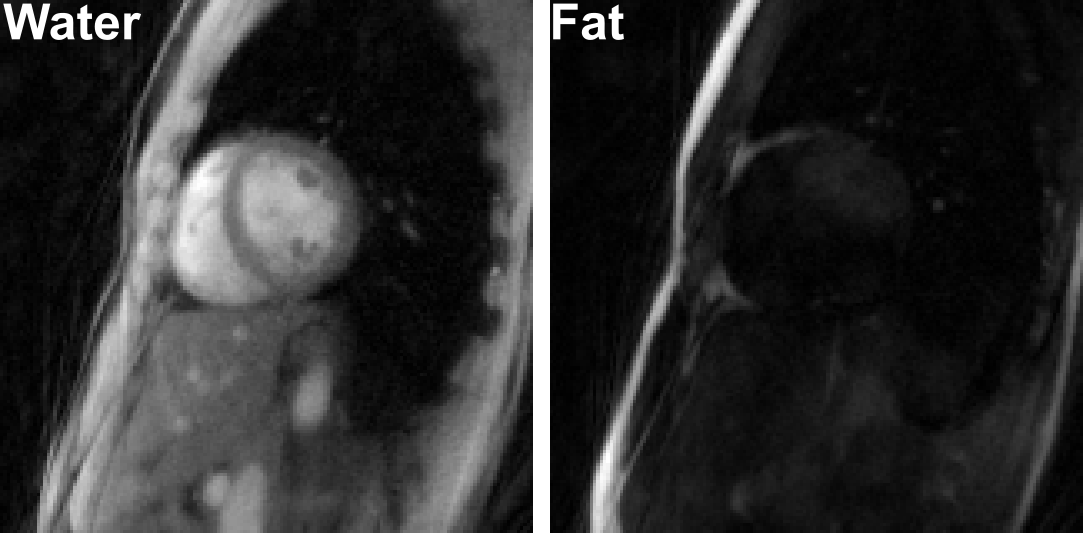
\includegraphics[width=0.7\textwidth]{fig/multi-echo-cardiac-menlinv-wf.png}
  \caption{Rough (left) water and (right) fat image calculated by the addition and subtraction between the first two echoes in \cref{Fig:multi-echo-cardiac-menlinv}.} \label{Fig:multi-echo-cardiac-menlinv-wf}
\end{figure}
One interesting phenomenon in \cref{Fig:multi-echo-cardiac-menlinv} is the appearance of ``white" fat signals in both the chest wall and areas surrounding the heart in the \nth{2} echo image, induced by the resonant-frequency difference between the water and fat nuclei. In principle, the difference in resonant frequencies between between two nuclei is 
\begin{equation}
  \Delta f = N_{\text{CS}} \cdot \frac{\gamma}{2\pi} \cdot B_0
\end{equation}
with $N_{\text{CS}}$ and $B_0$ being the chemical shift and the main magnetic field strength, respectively. Given the chemical shift between water and fat of \SI{3.5}{\ppm} \cite{1999_chem_shift}, the water-fat resonant frequency difference is
\begin{align}
  \Delta f_{\text{WF}} 
  &= \SI{3.5}{\ppm} \cdot \SI{42.576}{\mega\hertz\per\tesla} \cdot \SI{3}{\tesla} \nonumber \\
  &= \SI{447}{\hertz}
\end{align}
where ``W" and ``F" stand for water and fat, respectively. The phase shift between water and fat in an acquired echo is then given as
\begin{equation}
  \Delta \phi_{\text{WF}} (\text{TE}) = 2\pi \cdot \Delta f_{\text{WF}} \cdot \text{TE}
\end{equation}
Therefore, the \nth{1} and \nth{3} echo can be considered as ``opposed-phase" because the relative phase between water and fat is approximately $\pi$ and $3\pi$, respectively. On the contrary, the \nth{2} echo is ``in-phase" with $\Delta \phi_{\text{WF}} (\text{TE}_2) \approx 2\pi$. In principle, one echo (denoted as W $-$ F) can be acquired at the perfect ``opposed-phase" TE, and another (W $+$ F) acquired at the perfect ``in-phase" TE, so the water and fat component can be calculated via the addition and subtraction of these two echo images, as shown in \cref{Fig:multi-echo-cardiac-menlinv-wf}. This indicates the potential application of MEMS radial FLASH into more precise water-fat separation, where, in general, the water-fat signal acquired with multi-echo sequences can be written as
\begin{equation}
  \rho_l = \Big( \rho_\text{W} + \sum_{x=1}^{X} \rho_{\text{F},x} \cdot e^{-i 2\pi \cdot \Delta f_x \cdot t_l} \Big) \cdot e^{-i 2\pi \cdot \Delta f_{B0} \cdot t_l} \quad .
\end{equation}
Here, a multi-frequency-peak fat spectrum $\Delta f_x$ with $x \in [1,X]$ is used. $\rho_l$ is the $l$\textsuperscript{th} echo image. $\rho_\text{W}$ and $\rho_{\text{F},x}$ are the water and $x$\textsuperscript{th}-peak fat component, respectively. $\Delta f_{B0}$ is the main magnetic field inhomogeneity. $t_l$ is the $l$\textsuperscript{th} echo time. With the measured fat spectrum, $\rho_\text{W}$ and $\rho_{\text{F},x}$ can be estimated via the iterative least-square minimization (e.g.~see \cite{2004_IDEAL,2008_water_fat}).

\begin{figure}[tb]
  \centering
  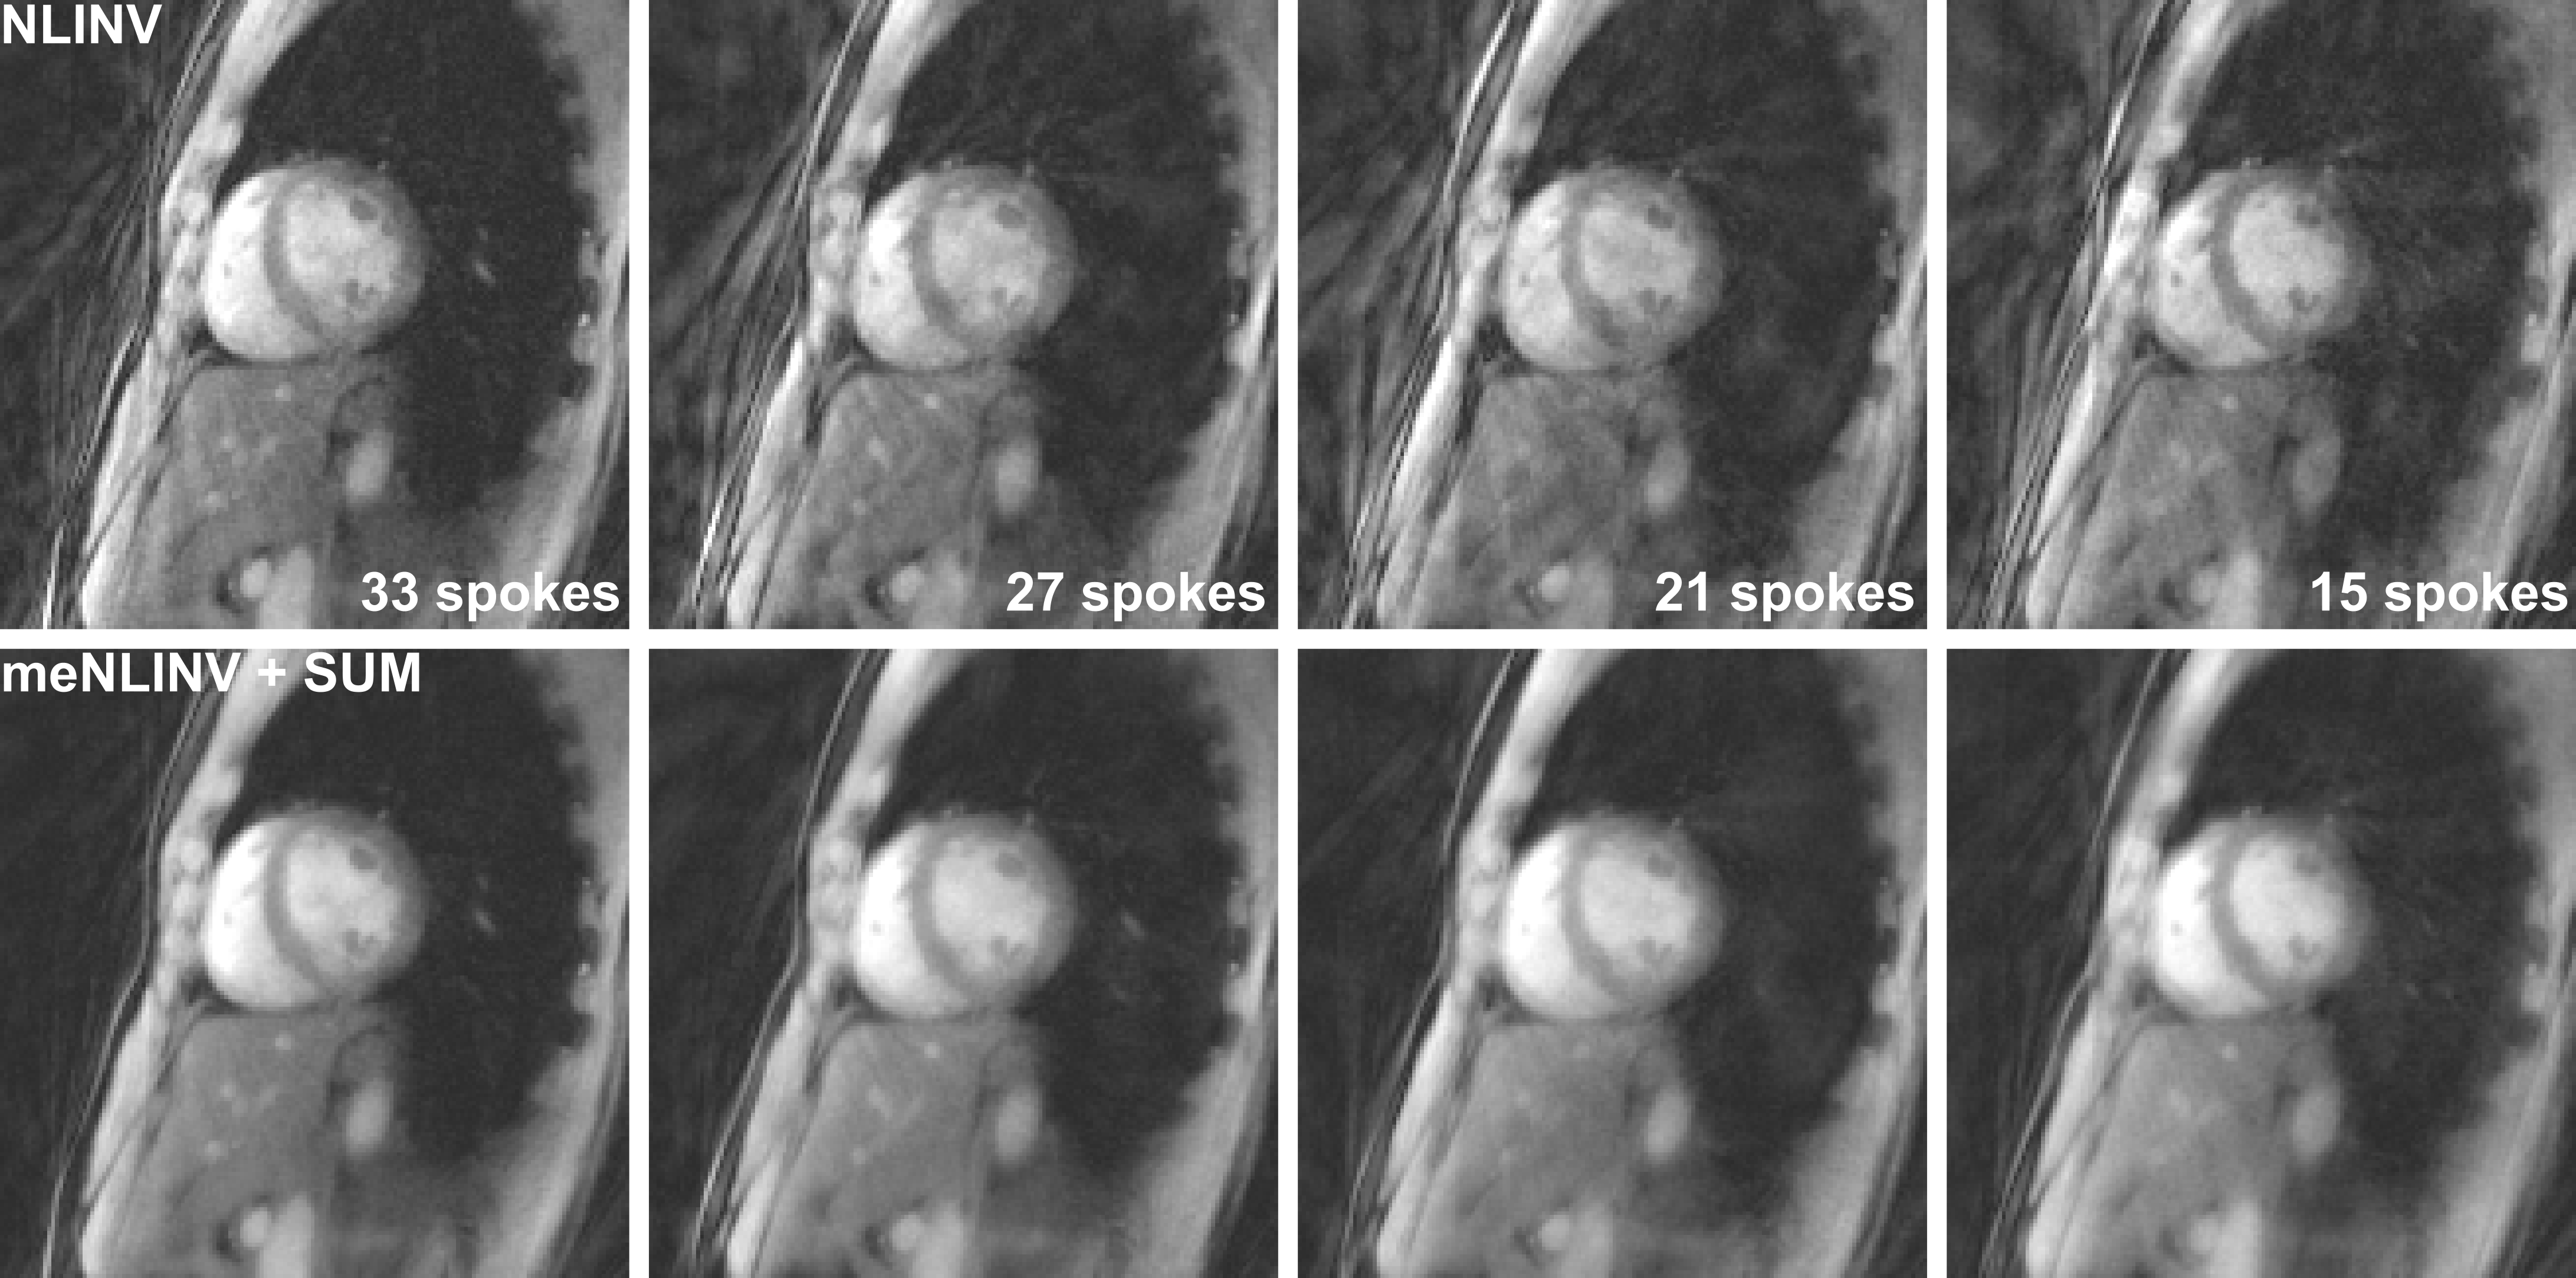
\includegraphics[width=\textwidth]{fig/multi-echo-cardiac-reco-comp.png}
  \caption{Comparisons of NLINV and meNLINV with a subsequent summation of echo images on the human heart (short-axis view) at diastole. The image columns represent reconstructed images acquired with \num{33}, \num{27}, \num{21}, and \num{15} spokes from left to right, respectively. The other acquisition parameters are given in \cref{Sec:me-method}.} \label{Fig:multi-echo-cardiac-reco-comp}
\end{figure}
\cref{Fig:multi-echo-cardiac-reco-comp} compares the standard NLINV and meNLINV with a subsequent summation of echo images (``meNLINV $+$ SUM") on the human heart (short-axis view) at diastole. All images are acquired with \num{3} echoes after each excitation using MEMS with linear view-ordering scheme. Due to fat-induced off-resonance phase differences among echoes, severe streaking artifacts appear around the chest wall and the heart in the standard NLINV reconstructed images. With the acquired number of spokes reduced, the myocardium becomes more blurred and signal loss happens in the area near to the middle cardiac vein. On the other hand, the ``meNLINV $+$ SUM" method can suppress the streaking artifacts caused by fat, but blurring and signal loss remain with reduced number of spokes. The blurring effect can probably be reduced by increasing the number of Newton steps, while signal intensity can be regained via proper off-resonance correction as described in \cref{Sec:me-iORC}, which, however, is not applicable in the extreme case, i.e., undersampled single-shot multi-echo radial FLASH. To overcome this problem, the standard NLINV with k-space off-resonance correction as a preprocessing step is preferable. Previous proposals dealt with k-space off-resonance correction requires either special orientations of sampled echoes \cite{1999_prMGE} or navigation signals \cite{2010_3D_rME}. An appropriate k-space off-resonance correction method which can be applied to multi-echo real-time MRI is still under investigation. An alternative for off-resonance correction is to develop a model-based reconstruction that jointly estimate the proton density, off-resonance frequency map, and $R_2^*$ relaxation map.

\section{Discussion}
This work demonstrates the successful development of two types of multi-echo radial FLASH sequences, multi-echo single-spoke and multi-echo multi-spoke. Preliminary results including the resolution phantom, human brain and heart demonstrate potential applicabilities of multi-echo radial FLASH, which range from anatomical imaging to water-fat separation, and to quantitative off-resonance frequency and $R_2^*$ relaxation mapping. Given the fact that this work only uses MEMS with linear view-ordering scheme and RF-spoiled radial FLASH, further optimizations of multi-echo view-ordering schemes, signal contrast, and acquisition parameters are demanded to move this sequence into routine use. Moreover, two types of reconstruction methods, the standard NLINV and meNLINV, are available for multi-echo radial sampled data. Optimal parameters for both methods, however, are still open questions. Nonetheless, even though preprocessing steps such as gradient delay correction and k-space off-resonance correction are beyond the scope of this work, they can still be helpful to improve image quality if they could be optimized for multi-echo data.

Further, this work combines multi-gradient-echo with radial sampling, which is not sensitive to the pronounced image artifacts in Cartesian EPI, e.g.~aliasing and off-resonance-induced spatial distortion. Off-resonance phase modulation, however, induces streaking and signal loss in multi-echo radial sampling. Although streakings are tolerable in certain cases (e.g.~fewer echoes and more spokes), an optimized MEMS radial sampling scheme and associated pragmatic off-resonance correction method are of great importance. Noteworthy, an interesting modification of the current multi-echo radial FLASH sequence would be to combine the blip and the readout ramp gradient, which can not only render a smooth transition between two successive echoes, but also shortens the echo spacing time.

An advantageous extension of the current NLINV reconstruction would be a model-based reconstruction that jointly estimates the proton density, off-resonance frequency, $R_2^*$ relaxation rate, and a set of coil sensitivity maps. The model-based reconstruction for real-time phase-contrast flow MRI in \cref{Chp:mir-pc} acts as a meaningful precursor study, which, however, requires a more general scaling strategy to make it a robust algorithm. When this is achieved, more endeavors could be made toward a model-based reconstruction for multi-echo radial FLASH. In fact, the model-based reconstruction discussed in this thesis integrates two types of image reconstruction, parallel imaging and quantitative parameter mapping. Apparently, it offers considerable advantages in terms of computational steps, but requires more effort on numerical optimization methods. Nonetheless, whether coils are reasonable to be included in the model or pre-calibrated is still an open question which could be answered with detailed comparisons.

\chapter{Summary and Outlook} \label{Chp:sum}

\section{Summary}
This thesis presents novel methodological developments in two major areas that both extend real-time MRI techniques and applications which are based on highly undersampled radial FLASH acquisitions and iterative image reconstruction as a nonlinear inverse (\acs{NLINV}) problem. The first new method is the exploration of advanced radial sampling schemes, namely the use of asymmetric echoes and multi-echo acquisitions, while the second contribution relates to advanced reconstruction principles, namely model-based reconstruction techniques that directly estimate parameter maps from raw data.

An asymmetric echo samples only a portion of the full echo and thus shortens the achievable echo time and repetition time. When applied to real-time phase-contrast flow MRI, its use not only improves temporal resolution, but also allows for the addition of flow-compensation gradients to suppress intra-voxel phase dispersion. Short echo times and first-order flow compensation for in-plane movements have been proven crucial for studies of patients with more complex flow patterns such as due to aortic valve insufficiency and partial stenosis.

Multi-echo radial sampling schemes offer multiple new opportunities ranging from a further speed-up of real-time data acquisitions to the reconstruction of quantitative parameter maps for off-resonance signal contributions and \acs{T2s} relaxation times. Two types of multi-echo radial FLASH sequences, i.e.~multi-echo single-spoke and multi-echo multi-spoke techniques, were developed and evaluated with the use of phantom and human studies. When compared to multi-echo single-spoke radial FLASH, the multi-spoke variant supplies a faster k-space coverage and various view-ordering schemes and therefore turns out to be promising for improved spatial and/or temporal resolution.

Partly in response to the new radial acquisition modes, the iterative image reconstruction demands new solutions. Thus, the second major part of this thesis was the development of image reconstruction techniques that advances well beyond the conventional \acs{NLINV} method for real-time MRI. For example, in case of real-time phase-contrast flow MRI, the computation of the desired phase-contrast (velocity) map requires at least two measurements with different velocity encodings. Conventionally, these measurements are treated as independent streams and reconstructed separately by NLINV (or Fourier transformation when using classical \acs{ECG}-synchronized acquisitions). The reconstructed images are then subject to a phase-difference calculation to obtain a phase-contrast map. For the past \num{30} years this two-step approach has been the only technical solution. However, the phase-difference calculation is prone to arbitrary phase noise in no or low MR signal areas and may even hamper the lumen definition and flow quantification. Therefore, a novel model-based reconstruction technique was developed which jointly estimates the anatomical image, the phase-contrast (velocity) map, and a set of coil sensitivity maps. The direct estimation of the phase-contrast map from the sets of raw data in combination with Tikhonov regularization ensures zero phase in no or low MR signal areas, which is clearly superior in sharpening vessel lumen and reducing streaking artifacts, especially for highly undersampled radial FLASH acquisitions. The technique was compared to the two-step NLINV approach and validated using a numerical phantom (ground truth), an experimental flow phantom, and measurements of human aortic blood flow.


\section{Future Work}

\subsection*{Model-based Reconstruction}
The current version of the advanced model-based reconstruction technique for real-time phase-contrast flow MRI to a certain degree still depends on the chosen scaling mechanism which is derived from the definition of the complex-difference image. This may be problematic in two more extreme situations, namely for very small phase differences (velocities) and in the presence of velocity aliasing. The former situation may increase the scaling value to such a degree that the concomitant regularization strength is weakened and noise accumulates in the estimate. On the other hand, the latter situation, which may be caused by the simultaneous presence of very high and very low flow, may lead to arbitrarily high phases in velocity-aliased regions and thus decrease the scaling, which in turn underestimates the resulting velocities. These scaling issues need to be resolved in order to make the model-based reconstruction technique a robust clinical tool.

As another potential extension, the integration of advanced regularizations, i.e., $L^1$-wavelet \cite{2008_NLINV_L1} and total (generalized) variation \cite{2012_NLINV_TGV}, into the model-based reconstruction may turn out to be advantageous and should be investigated. These non-quadratic regularizations offer better noise suppression, but require more complicated implementations. On the other hand, a prerequisite of the $L^1$-norm regularization is that the image to be regularized must be sparse. Fortunately, the complex-difference map is sparse by itself, requiring no sparsifying transform, so that this favorable feature may be exploited in a modified model-based reconstruction technique.

Further, as discussed in \cref{Chp:mir-pc}, the model-based reconstruction may be implemented with with different spatial encodings for the flow-compensated and flow-encoded dataset. In principle, this idea may help to increase the spatial resolution as more lines in k-space are available for image reconstruction. Moreover, respective reconstruction may effectively double the temporal resolution when combining such acquisitions with a two-sided flow encoding scheme and a sliding window which shifts the reconstruction by only one dataset rather than two in all current methods.

Finally, the model-based reconstruction can be greatly accelerated via a multi-\acs{GPU} implementation to allow for extensive clinic trials. 

\subsection*{Multi-Echo Radial FLASH}
The developments described in \cref{Chp:multi-echo} primarily focused on multi-echo multi-spoke acquisitions with linear view ordering for the convenience of image reconstruction. However, other view-ordering schemes need to be further investigated. Imaging parameters such as flip angle, bandwidth, number of spokes and echoes, echo spacing, and potential contrasts need to be thoroughly studied as well. Moreover, because this sequence is compatible with asymmetric echoes, it needs to be evaluated whether such a combination may further speed up acquisitions, or offers specific applications with variable echo spacings. 

With the implementation of more and more complex gradient switching schemes, it may also become necessary to develop special gradient delay corrections and k-space off-resonance corrections to maintain or improve image qualities. For multi-echo image reconstructions, the NLINV variants also require further optimization with regard to the number of Newton steps, temporal regularization, and initialization. As an ultimate goal, quantitative parametric mapping of \acs{T2s} relaxation times and off-resonance frequencies should be accomplished by a suitable model-based reconstruction technique. 

Taken together, a successful validation of undersampled multi-echo multi-spoke acquisitions with respective image reconstructions could certainly advance the general concept of real-time MRI, not only with respect to temporal resolution but also with respect to novel (dynamic) contrasts exploiting the \acs{T2s}-weighted signal decay and off-resonance phase modulation. These factors have various clinical applications such as the identification of hemorrhage and calcification, access to tissue oxygenation, susceptibility-weighted imaging, and water-fat separation.


%\appendix
\begin{appendices}
\chapter{Analytical Phantoms with Multiple Receiver Coils}
\label{Chp:AnalCoil}

The magnetic field generated at position $\vec{r}$ by the coil with steady current $I$ is given by Biot-Savart law,
\begin{equation} \label{Equ:BSlaw}
  B(\vec{r}) = \frac{\mu_0 I}{4\pi} \oint_{\text{coil}} \frac{d\vec{u} \times (\vec{u} - \vec{r})}{\norm{\vec{u}-\vec{r}}^3}
\end{equation}
Therefore, complex coil sensitivity maps can be simulated using \cref{Equ:BSlaw} and the coil geometry. To integrate coil sensitivity maps into analytical Fourier transform, mathematical approximation of the maps are necessary. Because it is well known that coil sensitivity maps are smooth and slowly-varying, so polynomial and sinusoidal models \cite{1999_SENSE,2012_analSim} are commonly used for approximation. 

On the one hand, the sinusoidal model represents the coil sensitivity map with complex exponentials expanding over a range of low spatial frequencies,
\begin{equation} \label{Equ:coil_sinu}
  c(\vec{r}) = \sum_{\vec{v}} C_{\vec{v}} \cdot e^{i \vec{r} \cdot \vec{v}}
\end{equation}
where $\vec{v}$ is a set of low spatial frequencies used to constrain the smoothness of the coil sensitivity map $c(\vec{v})$, $\vec{r}$ the Cartesian grids within the FOV, and $C_{\vec{v}}$ the coefficients of the complex exponentials. Therefore, plugging \cref{Equ:coil_sinu} into \cref{Equ:cont_FT_rho_coil} yields 
\begin{equation} \label{Equ:cont_FT_rho_sinu_coil}
\begin{aligned}
  y_j(t) 
  & = \int_{\vec{r}} c_j(\vec{r}) \cdot \rho(\vec{r}) \cdot e^{-i 2\pi \vec{k}(t) \vec{r}} d\vec{r} \\
  & = \int_{\vec{r}} \sum_{\vec{v}} C_{\vec{v}} \cdot e^{i \vec{r} \cdot \vec{v}} \cdot \rho(\vec{r}) \cdot e^{-i 2\pi \vec{k}(t) \vec{r}} d\vec{r} \\
  & = \sum_{\vec{v}} C_{\vec{v}} \int_{\vec{r}} \rho(\vec{r}) \cdot e^{-i [2\pi \vec{k}(t) - \vec{v}] \cdot \vec{r}} d\vec{r}
\end{aligned}
\end{equation}
where the integration part is actually a translation of \cref{Equ:sum_aFT_rho}, so the analytical form of \cref{Equ:cont_FT_rho_sinu_coil} is
\begin{equation} \label{Equ:sum_aFT_rho_coil}
  y(\vec{k}) = \sum_{m} I_m \sum_{\vec{v}} s_{\vec{v}} \cdot A_m(2\pi \vec{k} - \vec{v})
\end{equation}

On the ohter hand, for the polynomial model, the coil sensitivity map is approximated by a polynomial function with a degree $D$,
\begin{equation} \label{Equ:coil_poly}
  c(\vec{r}) = \sum_{d=0}^{D} \sum_{|\vec{\alpha}|=d} C_{d,\vec{\alpha}} \cdot \vec{r}^{\vec{\alpha}}
\end{equation}
where $C_{d,\vec{\alpha}}$ is the coefficients of polynomials, and $\vec{\alpha}$ a two-element vector representing the dimension of FOV. Therefore, \cref{Equ:cont_FT_rho_coil} becomes
\begin{equation} \label{Equ:cont_FT_rho_poly_coil}
\begin{aligned}
  y_j(t) 
  & = \int_{\vec{r}} c_j(\vec{r}) \cdot \rho(\vec{r}) \cdot e^{-i 2\pi \vec{k}(t) \vec{r}} d\vec{r} \\
  & = \int_{\vec{r}} \sum_{d=0}^D \sum_{|\vec{\alpha}|=d} C_{d,\vec{\alpha}} \cdot \vec{r}^{\vec{\alpha}} \cdot \rho(\vec{r}) \cdot e^{-i 2\pi \vec{k}(t) \vec{r}} d\vec{r} \\
  & = \sum_{d=0}^D \sum_{|\vec{\alpha}|=d} C_{d,\vec{\alpha}} \int_{\vec{r}} \vec{r}^{\vec{\alpha}} \cdot \rho(\vec{r}) \cdot e^{-i 2\pi \vec{k}(t) \vec{r}} d\vec{r}
\end{aligned}
\end{equation}
where $\abs{\vec{\alpha}}$ denotes the sum of all elements in the vector $\vec{\alpha}$. As derived in \cite{2012_analSim}, this integration is equivalent to the $\abs{\vec{\alpha}}$-order partial derivatives of the analytical Fourier transform, which can be calculated via the recursive decomposition. 




\end{appendices}

% ==============================================================
\backmatter
% - bibliography, glossary and index would go here.
% - list of acronyms
% - index
% ==============================================================
\cleardoublepage
\bibliographystyle{unsrtnat}
\refstepcounter{chapter}
\addcontentsline{toc}{chapter}{\bibname}
\bibliography{C_Ref}
%\printbibliography

\chapter{Abbreviations}
\begin{acronym}
  \acro{ACS}{Auto-Calibration Signal}
  \acro{ADC}{Analog-to-Digital Converter}
  \acro{BOLD}{Blood-Oxygen-Level Dependent}
  \acro{BW}{BandWidth}
  \acro{bSSFP}{balanced Steady-State Free Precession} 
  \acro{CG}{Conjugate Gradient} 
  \acro{CMR}{Cardiovascular Magnetic Resonance} 
%  \acro{CPU}{Central Processing Unit}
%  \acro{CT}{Computed Tomography} 
%  \acro{DCF}{Density Compensation Function} 
  \acro{DFT}{Discrete Fourier Transform} 
  \acro{ECG}{ElectroCardioGraph} 
%  \acro{EMF}{ElectroMotive Force} 
  \acro{EPI}{echo-planar imaging}
  \acro{ESP}{Echo SPacing} 
  \acro{ETL}{Echo Train Length}
%  \acro{FC}{Flow-Compensation} 
%  \acro{FE}{Flow-Encoding} 
  \acro{FFT}{Fast Fourier Transform} 
  \acro{FID}{Free Induction Decay} 
  \acro{FLASH}{Fast Low Angle SHot} 
  \acro{fMRI}{functional Magnetic Resonance Imaging} 
  \acro{FOV}{Field Of View} 
  \acro{GPU}{Graphics Processing Unit} 
  \acro{GRAPPA}{GeneRalized Autocalibrating Partially Parallel Acquisitions} 
%  \acro{GRASE}{GRAdient and Spin-Echo}
  \acro{IRGNM}{Iteratively Regularized Gauss-Newton Method} 
  \acro{JSENSE}{Joint SENSitivity Encoding}
  \acro{KESA}{K-space Energy Spectrum Analysis}
  \acro{MEMS}{Multi-Echo Multi-Spoke}
  \acro{MESS}{Multi-Echo Single-Spoke}
  \acro{MRI}{Magnetic Resonance Imaging}  
  \acro{NLINV}{NonLinear INVersion} 
  \acro{NMR}{Nuclear Magnetic Resonance} 
  \acro{NUFFT}{Non-Uniform Fast Fourier Transform}
  \acro{ORC}{Off-Resonance Correction} 
%  \acro{PET}{Positron Emission Tomography}
  \acro{PD}{Proton Density} 
  \acro{POCS}{Projection Onto Convex Sets} 
  \acro{PROPELLER}{Periodically Rotated Overlapping ParallEL Lines with Enhanced Reconstruction} 
  \acro{PSF}{Point Spread Function} 
  \acro{RARE}{Rapid Acquisition with Relaxation Enhancement} 
  \acro{RF}{Radio-Frequency} 
  \acro{ROI}{Region-Of-Interest} 
  \acro{SENSE}{SENSitivity Encoding} 
  \acro{SMASH}{SiMultaneously Acquisition of Spatial Harmonics} 
  \acro{SNR}{Signal-to-Noise Ratio} 
%  \acro{SPIDER}{Steady-state Projection Imaging with Dynamic Echo-train Readout}
  \acro{T1}[$T_1$]{spin-lattice relaxation time}
  \acro{T2}[$T_2$]{spin-spin relaxation time}
  \acro{T2s}[$T_2^*$]{effective spin-spin relaxation time}
  \acro{TE}{Echo Time} 
%  \acro{TMJ}{TemporoMandibular Joint} 
  \acro{TR}{Repetition Time} 
  \acro{VENC}{Velocity ENCoding} 
\end{acronym}


\chapter{Curriculum Vitae}

\section*{Personal Data}
\begin{tabular}{ p{.15\textwidth}p{.80\textwidth} }
  Name: & Zhengguo Tan \\
  Date of Birth: & August 7, 1985 \\
  Place of Birth: & Guangdong, China \\
  Nationality: & Chinese \\
  Email: & \href{mailto:zhengguo.tan@icloud.com}{zhengguo.tan@icloud.com} \\
         & \href{mailto:ztan@gwdg.de}{ztan@gwdg.de} \\
\end{tabular}

\section*{Education}
\begin{tabular}{ p{.15\textwidth}p{.80\textwidth} }
  2012 - present & Dr.~rer.~nat., Physics, Georg-August-Universit\"{a}t G\"{o}ttingen, Germany \\
  2010 - 2012    & Master of Science, Biomedical Engineering, Duke University, USA \\
  2005 - 2010    & Bachelor of Science, Biomedical Engineering, Zhejiang University, China \\
  2002 - 2005    & High School Diploma, Huazhou No.1 High School, Guangdong, China \\
\end{tabular}

\section*{Professional Experience}
\begin{tabular}{ p{.15\textwidth}p{.80\textwidth} }
  2012 - present & Research Assistant at Biomedizinische NMR Forschungs GmbH, G\"{o}ttingen \\
  2011 - 2012    & Student Assistant at Brain Imaging and Analysis Center, Duke University \\
  2010 - 2011    & Student Assistant at Carl E. Ravin Advanced Imaging Lab, Duke University \\
  2009           & Undergraduate Student Assistant at Biomedical Imaging and Biosignal Analysis Lab, University of Nebraska - Lincoln \\
\end{tabular}

\section*{Teaching Experience}
\begin{tabular}{ p{.15\textwidth}p{.80\textwidth} }
  2012 - 2015 & Basic Principle of MRI and Real-Time MRI, G\"{o}ttingen Graduate School for Neurosciences, Biophysics, and Molecular Biosciences (GGNB) \\
  2014 & Scientific Computing II, Physics Faculty, Georg-August-Universit\"{a}t G\"{o}ttingen \\
\end{tabular}

\section*{Affiliations}
\begin{tabular}{ p{.15\textwidth}p{.80\textwidth} }
  2014 - present & Trainee Member at the International Society for Magnetic Resonance in Medicine (ISMRM) \\
  2013 - 2014    & Trainee Member at the European Society for Magnetic Resonance in Medicine and Biology (ESMRMB) \\
\end{tabular}

\section*{Awards}
\begin{tabular}{ p{.15\textwidth}p{.80\textwidth} }
  2016        & ISMRM Educational Stipends \\
  2010 - 2012 & Graduate School Fellowship, Duke University \\
  2008        & \nth{2} Prize, Electronic System Design Contest, Zhejiang University \\
  2006        & \nth{2} Prize, Outstanding Undergraduate Scholarship, Zhejiang University \\
\end{tabular}

\section*{Miscellaneous}
\begin{tabular}{ p{.15\textwidth}p{.80\textwidth} }
  2006 - 2007 & Table Tennis Team Leader of College of Biomedical Engineering in Merit Cup, Zhejiang University \\
\end{tabular}

\chapter{List of Publications}

\section*{Journal Publications}
\begin{etaremune}
\item Zhengguo Tan, Volkert Roeloffs, Dirk Voit, Arun A Joseph, Markus Untenberger, K Dietmar Merboldt and Jens Frahm, \textbf{Model-based reconstruction for real-time phase-contrast flow MRI: Improved spatiotemporal accuracy}, \textit{Magnetic Resonance in Medicine}, 2016. \href{http://dx.doi.org/10.1002/mrm.26192}{DOI: 10.1002/mrm.26192}
\item Markus Untenberger$\dagger$, Zhengguo Tan$\dagger$, Dirk Voit, Arun A Joseph, Volkert Roeloffs, K Dietmar Merboldt, Sebastian Schaetz and Jens Frahm, \textbf{Advances in real-time phase-contrast flow MRI using asymmetric radial gradient echoes}, \textit{Magnetic Resonance in Medicine}, 2015. \href{http://dx.doi.org/10.1002/mrm.25696}{DOI: 10.1002/mrm.25696} ($\dagger$ Equal Contribution)
\end{etaremune}


\section*{Conference Contributions}
\begin{etaremune}
\item Zhengguo Tan, Volkert Roeloffs, Dirk Voit, Arun A Joseph, Markus Untenberger, K Dietmar Merboldt and Jens Frahm, \textbf{Model-based reconstruction for real-time phase-contrast flow MRI -- Improved spatiotemporal accuracy}, In \textit{Proceedings of the \nth{24} ISMRM}, Singapore, 2016. (power pitch)
\item Zhengguo Tan and Jens Frahm, \textbf{Model-based reconstruction for real-time phase-contrast flow MRI -- Improved spatiotemporal accuracy}, \textit{Departmental Poster Presentation to the Scientific Advisory Board (SAB) of MPIBPC}, 2015.
\item Zhengguo Tan, \textbf{Model-based reconstruction for real-time phase-contrast flow MRI}, talk on \textit{THIRD INFINITY}, G\"{o}ttingen, 2015.
\item Tom Hilbert, Tobias Kober, Tilman J Sumpf, Zhengguo Tan, Jens Frahm, Pavel Falkovskiy, Heiko Meyer, Rolf Bendl, Jean-Philippe Thiran and Reto Meuli, \textbf{MARTINI and GRAPPA -- When speed is taste}, In \textit{Proceedings of the \nth{22} ISMRM}, Milan, Italy, page 4077, 2014.
\item Zhengguo Tan, Dirk Voit and Jens Frahm, \textbf{Analytical multi-echo radial FLASH MRI simulation}, \textit{\nth{3} GGNB Science Day}, G\"{o}ttingen, 2013.
\item Zhengguo Tan and Nan-Kuei Chen, \textbf{Application of k-space energy spectrum analysis to artifact correction in PROPELLER MRI}, In \textit{Proceedings of the \nth{20} ISMRM}, Melbourne, Australia, page 2422, 2012.
\end{etaremune}




\end{document}